\documentclass[twoside]{book}

% Packages required by doxygen
\usepackage{fixltx2e}
\usepackage{calc}
\usepackage{doxygen}
\usepackage{graphicx}
\usepackage[utf8]{inputenc}
\usepackage{makeidx}
\usepackage{multicol}
\usepackage{multirow}
\PassOptionsToPackage{warn}{textcomp}
\usepackage{textcomp}
\usepackage[nointegrals]{wasysym}
\usepackage[table]{xcolor}

% Font selection
\usepackage[T1]{fontenc}
\usepackage{mathptmx}
\usepackage[scaled=.90]{helvet}
\usepackage{courier}
\usepackage{amssymb}
\usepackage{sectsty}
\renewcommand{\familydefault}{\sfdefault}
\allsectionsfont{%
  \fontseries{bc}\selectfont%
  \color{darkgray}%
}
\renewcommand{\DoxyLabelFont}{%
  \fontseries{bc}\selectfont%
  \color{darkgray}%
}
\newcommand{\+}{\discretionary{\mbox{\scriptsize$\hookleftarrow$}}{}{}}

% Page & text layout
\usepackage{geometry}
\geometry{%
  a4paper,%
  top=2.5cm,%
  bottom=2.5cm,%
  left=2.5cm,%
  right=2.5cm%
}
\tolerance=750
\hfuzz=15pt
\hbadness=750
\setlength{\emergencystretch}{15pt}
\setlength{\parindent}{0cm}
\setlength{\parskip}{0.2cm}
\makeatletter
\renewcommand{\paragraph}{%
  \@startsection{paragraph}{4}{0ex}{-1.0ex}{1.0ex}{%
    \normalfont\normalsize\bfseries\SS@parafont%
  }%
}
\renewcommand{\subparagraph}{%
  \@startsection{subparagraph}{5}{0ex}{-1.0ex}{1.0ex}{%
    \normalfont\normalsize\bfseries\SS@subparafont%
  }%
}
\makeatother

% Headers & footers
\usepackage{fancyhdr}
\pagestyle{fancyplain}
\fancyhead[LE]{\fancyplain{}{\bfseries\thepage}}
\fancyhead[CE]{\fancyplain{}{}}
\fancyhead[RE]{\fancyplain{}{\bfseries\leftmark}}
\fancyhead[LO]{\fancyplain{}{\bfseries\rightmark}}
\fancyhead[CO]{\fancyplain{}{}}
\fancyhead[RO]{\fancyplain{}{\bfseries\thepage}}
\fancyfoot[LE]{\fancyplain{}{}}
\fancyfoot[CE]{\fancyplain{}{}}
\fancyfoot[RE]{\fancyplain{}{\bfseries\scriptsize Generated on Mon Sep 14 2015 08\+:57\+:08 for libtoxcore by Doxygen }}
\fancyfoot[LO]{\fancyplain{}{\bfseries\scriptsize Generated on Mon Sep 14 2015 08\+:57\+:08 for libtoxcore by Doxygen }}
\fancyfoot[CO]{\fancyplain{}{}}
\fancyfoot[RO]{\fancyplain{}{}}
\renewcommand{\footrulewidth}{0.4pt}
\renewcommand{\chaptermark}[1]{%
  \markboth{#1}{}%
}
\renewcommand{\sectionmark}[1]{%
  \markright{\thesection\ #1}%
}

% Indices & bibliography
\usepackage{natbib}
\usepackage[titles]{tocloft}
\setcounter{tocdepth}{3}
\setcounter{secnumdepth}{5}
\makeindex

% Hyperlinks (required, but should be loaded last)
\usepackage{ifpdf}
\ifpdf
  \usepackage[pdftex,pagebackref=true]{hyperref}
\else
  \usepackage[ps2pdf,pagebackref=true]{hyperref}
\fi
\hypersetup{%
  colorlinks=true,%
  linkcolor=blue,%
  citecolor=blue,%
  unicode%
}

% Custom commands
\newcommand{\clearemptydoublepage}{%
  \newpage{\pagestyle{empty}\cleardoublepage}%
}


%===== C O N T E N T S =====

\begin{document}

% Titlepage & ToC
\hypersetup{pageanchor=false,
             bookmarks=true,
             bookmarksnumbered=true,
             pdfencoding=unicode
            }
\pagenumbering{roman}
\begin{titlepage}
\vspace*{7cm}
\begin{center}%
{\Large libtoxcore }\\
\vspace*{1cm}
{\large Generated by Doxygen 1.8.8}\\
\vspace*{0.5cm}
{\small Mon Sep 14 2015 08:57:08}\\
\end{center}
\end{titlepage}
\clearemptydoublepage
\tableofcontents
\clearemptydoublepage
\pagenumbering{arabic}
\hypersetup{pageanchor=true}

%--- Begin generated contents ---
\chapter{av\+\_\+api}
\label{md_docs_av_api}
\hypertarget{md_docs_av_api}{}
\#\+A/\+V A\+P\+I reference

\subsection*{Take toxmsi/phone.\+c as a reference}

\subsubsection*{Initialization\+:}

``` phone\+\_\+t$\ast$ init\+Phone(uint16\+\_\+t \+\_\+listen\+\_\+port, uint16\+\_\+t \+\_\+send\+\_\+port); ```

function initializes sample phone. \+\_\+listen\+\_\+port and \+\_\+send\+\_\+port are variables only meant for local testing. You will not have to do anything regarding to that since everything will be started within a mesenger.

Phone requires one msi session and two rtp sessions ( one for audio and one for video ).

``` msi\+\_\+session\+\_\+t$\ast$ msi\+\_\+init\+\_\+session( void$\ast$ \+\_\+core\+\_\+handler, const uint8\+\_\+t$\ast$ \+\_\+user\+\_\+agent ); ```

initializes msi session. Params\+:

``` void$\ast$ \+\_\+core\+\_\+handler -\/ pointer to an object handling networking, const uint8\+\_\+t$\ast$ \+\_\+user\+\_\+agent -\/ string describing phone client version. ```

Return value\+: msi\+\_\+session\+\_\+t$\ast$ -\/ pointer to a newly created msi session handler.

\subsubsection*{msi\+\_\+session\+\_\+t reference\+:}

How to handle msi session\+: Controlling is done via callbacks and action handlers. First register callbacks for every state/action received and make sure N\+O\+T T\+O P\+L\+A\+C\+E S\+O\+M\+E\+T\+H\+I\+N\+G L\+I\+K\+E L\+O\+O\+P\+S T\+H\+A\+T T\+A\+K\+E\+S A L\+O\+T O\+F T\+I\+M\+E T\+O E\+X\+E\+C\+U\+T\+E; every callback is being called directly from event loop. You can find examples in phone.\+c.

Register callbacks\+: ``` void msi\+\_\+register\+\_\+callback\+\_\+call\+\_\+started ( M\+C\+A\+L\+L\+B\+A\+C\+K ); void msi\+\_\+register\+\_\+callback\+\_\+call\+\_\+canceled ( M\+C\+A\+L\+L\+B\+A\+C\+K ); void msi\+\_\+register\+\_\+callback\+\_\+call\+\_\+rejected ( M\+C\+A\+L\+L\+B\+A\+C\+K ); void msi\+\_\+register\+\_\+callback\+\_\+call\+\_\+ended ( M\+C\+A\+L\+L\+B\+A\+C\+K );

void msi\+\_\+register\+\_\+callback\+\_\+recv\+\_\+invite ( M\+C\+A\+L\+L\+B\+A\+C\+K ); void msi\+\_\+register\+\_\+callback\+\_\+recv\+\_\+ringing ( M\+C\+A\+L\+L\+B\+A\+C\+K ); void msi\+\_\+register\+\_\+callback\+\_\+recv\+\_\+starting ( M\+C\+A\+L\+L\+B\+A\+C\+K ); void msi\+\_\+register\+\_\+callback\+\_\+recv\+\_\+ending ( M\+C\+A\+L\+L\+B\+A\+C\+K ); void msi\+\_\+register\+\_\+callback\+\_\+recv\+\_\+error ( M\+C\+A\+L\+L\+B\+A\+C\+K );

void msi\+\_\+register\+\_\+callback\+\_\+requ\+\_\+timeout ( M\+C\+A\+L\+L\+B\+A\+C\+K ); ```

M\+C\+A\+L\+L\+B\+A\+C\+K is defined as\+: void ({\itshape callback) (void} \+\_\+arg) msi\+\_\+session\+\_\+t$\ast$ handler is being thrown as \+\_\+arg so you can use that and \+\_\+agent\+\_\+handler to get to your own phone handler directly from callback.

Actions\+:

``` int msi\+\_\+invite ( msi\+\_\+session\+\_\+t$\ast$ \+\_\+session, call\+\_\+type \+\_\+call\+\_\+type, uint32\+\_\+t \+\_\+timeoutms ); ```

Sends call invite. Before calling/sending invite msi\+\_\+session\+\_\+t\+::\+\_\+friend\+\_\+id is needed to be set or else it will not work. \+\_\+call\+\_\+type is type of the call ( Audio/\+Video ) and \+\_\+timeoutms is how long will poll wait until request is terminated.

``` int msi\+\_\+hangup ( msi\+\_\+session\+\_\+t$\ast$ \+\_\+session ); ``` Hangs up active call

``` int msi\+\_\+answer ( msi\+\_\+session\+\_\+t$\ast$ \+\_\+session, call\+\_\+type \+\_\+call\+\_\+type ); ``` Answer incomming call. \+\_\+call\+\_\+type set's callee call type.

``` int msi\+\_\+cancel ( msi\+\_\+session\+\_\+t$\ast$ \+\_\+session ); ``` Cancel current request.

``` int msi\+\_\+reject ( msi\+\_\+session\+\_\+t$\ast$ \+\_\+session ); ``` Reject incomming call.

\subsubsection*{Now for rtp\+:}

You will need 2 sessions; one for audio one for video. You start them with\+: ``` rtp\+\_\+session\+\_\+t$\ast$ rtp\+\_\+init\+\_\+session ( int \+\_\+max\+\_\+users, int \+\_\+multi\+\_\+session ); ```

Params\+: ``` int \+\_\+max\+\_\+users -\/ max users. -\/1 if undefined int \+\_\+multi\+\_\+session -\/ any positive number means uses multi session; -\/1 if not. ```

Return value\+: ``` rtp\+\_\+session\+\_\+t$\ast$ -\/ pointer to a newly created rtp session handler. ```

\subsubsection*{How to handle rtp session\+:}

Take a look at ``` void$\ast$ phone\+\_\+handle\+\_\+media\+\_\+transport\+\_\+poll ( void$\ast$ \+\_\+hmtc\+\_\+args\+\_\+p ) in phone.\+c ``` on example. Basically what you do is just receive a message via\+: ``` struct rtp\+\_\+msg\+\_\+s$\ast$ rtp\+\_\+recv\+\_\+msg ( rtp\+\_\+session\+\_\+t$\ast$ \+\_\+session ); ```

and then you use payload within the rtp\+\_\+msg\+\_\+s struct. Don't forget to deallocate it with\+: void rtp\+\_\+free\+\_\+msg ( rtp\+\_\+session\+\_\+t$\ast$ \+\_\+session, struct rtp\+\_\+msg\+\_\+s$\ast$ \+\_\+msg ); Receiving should be thread safe so don't worry about that.

When you capture and encode a payload you want to send it ( obviously ).

first create a new message with\+: ``` struct rtp\+\_\+msg\+\_\+s$\ast$ rtp\+\_\+msg\+\_\+new ( rtp\+\_\+session\+\_\+t$\ast$ \+\_\+session, const uint8\+\_\+t$\ast$ \+\_\+data, uint32\+\_\+t \+\_\+length ); ```

and then send it with\+: ``` int rtp\+\_\+send\+\_\+msg ( rtp\+\_\+session\+\_\+t$\ast$ \+\_\+session, struct rtp\+\_\+msg\+\_\+s$\ast$ \+\_\+msg, void$\ast$ \+\_\+core\+\_\+handler ); ```

\+\_\+core\+\_\+handler is the same network handler as in msi\+\_\+session\+\_\+s struct.

\subsection*{A/\+V initialization\+:}

``` int init\+\_\+receive\+\_\+audio(codec\+\_\+state $\ast$cs); int init\+\_\+receive\+\_\+video(codec\+\_\+state $\ast$cs); Initialises the A/\+V decoders. On failure it will print the reason and return 0. On success it will return 1.

int init\+\_\+send\+\_\+audio(codec\+\_\+state $\ast$cs); int init\+\_\+send\+\_\+video(codec\+\_\+state $\ast$cs); Initialises the A/\+V encoders. On failure it will print the reason and return 0. On success it will return 1. init\+\_\+send\+\_\+audio will also let the user select an input device. init\+\_\+send\+\_\+video will determine the webcam's output codec and initialise the appropriate decoder.

int video\+\_\+encoder\+\_\+refresh(codec\+\_\+state $\ast$cs, int bps); Reinitialises the video encoder with a new bitrate. ffmpeg does not expose the needed V\+P8 feature to change the bitrate on the fly, so this serves as a workaround. In the future, V\+P8 should be used directly and ffmpeg should be dropped from the dependencies. The variable bps is the required bitrate in bits per second. ```

\subsubsection*{A/\+V encoding/decoding\+:}

``` void $\ast$encode\+\_\+video\+\_\+thread(void $\ast$arg); ``` Spawns the video encoding thread. The argument should hold a pointer to a codec\+\_\+state. This function should only be called if video encoding is supported (when init\+\_\+send\+\_\+video returns 1). Each video frame gets encoded into a packet, which is sent via R\+T\+P. Every 60 frames a new bidirectional interframe is encoded. ``` void $\ast$encode\+\_\+audio\+\_\+thread(void $\ast$arg); ``` Spawns the audio encoding thread. The argument should hold a pointer to a codec\+\_\+state. This function should only be called if audio encoding is supported (when init\+\_\+send\+\_\+audio returns 1). Audio frames are read from the selected audio capture device during intitialisation. This audio capturing can be rerouted to a different device on the fly. Each audio frame is encoded into a packet, and sent via R\+T\+P. All audio frames have the same amount of samples, which is defined in A\+V\+\_\+codec.\+h. ``` int video\+\_\+decoder\+\_\+refresh(codec\+\_\+state $\ast$cs, int width, int height); ``` Sets the S\+D\+L window dimensions and creates a pixel buffer with the requested size. It also creates a scaling context, which will be used to convert the input image format to Y\+U\+V420\+P.

``` void $\ast$decode\+\_\+video\+\_\+thread(void $\ast$arg); ``` Spawns a video decoding thread. The argument should hold a pointer to a codec\+\_\+state. The codec\+\_\+state is assumed to contain a successfully initialised video decoder. This function reads video packets and feeds them to the video decoder. If the video frame's resolution has changed, video\+\_\+decoder\+\_\+refresh() is called. Afterwards, the frame is displayed on the S\+D\+L window. ``` void $\ast$decode\+\_\+audio\+\_\+thread(void $\ast$arg); ``` Spawns an audio decoding thread. The argument should hold a pointer to a codec\+\_\+state. The codec\+\_\+state is assumed to contain a successfully initialised audio decoder. All received audio packets are pushed into a jitter buffer and are reordered. If there is a missing packet, or a packet has arrived too late, it is treated as a lost packet and the audio decoder is informed of the packet loss. The audio decoder will then try to reconstruct the lost packet, based on information from previous packets. Audio is played on the default Open\+A\+L output device.

If you have any more qustions/bug reports/feature request contact the following users on the irc channel \#tox-\/dev on irc.\+freenode.\+net\+: For R\+T\+P and M\+S\+I\+: mannol For audio and video\+: Martijnvdc 
\chapter{Group-\/\+Chats}
\label{md_docs__group-_chats}
\hypertarget{md_docs__group-_chats}{}
Group chats.

Note\+: we assume everyone in the chat trusts each other.

These group chats work by temporarily adding the 4 \char`\"{}closest\char`\"{} people defined by a distance function in group.\+c in order to form a circle of connected peers. These peers then relay messages to each other.

A friend invites another friend to a group chat by sending them an invite packet. The friend either ignores the invite or responds with a response packet if he wants to join the chat. The friend invite contains the type of groupchat (text only, A/\+V) the friend is being invited to.

T\+O\+D\+O\+: write more of this.

\subsection*{Protocol}

Invite packets\+: Invite packet\+: \mbox{[}uint8\+\_\+t id 96\mbox{]}\mbox{[}uint8\+\_\+t id 0\mbox{]}\mbox{[}uint16\+\_\+t group chat number\mbox{]}\mbox{[}33 bytes group chat identifier\mbox{[}1 byte type\mbox{]}\mbox{[}32 bytes id\mbox{]}\mbox{]}

Response packet \mbox{[}uint8\+\_\+t id 96\mbox{]}\mbox{[}uint8\+\_\+t id 1\mbox{]}\mbox{[}uint16\+\_\+t group chat number(local)\mbox{]}\mbox{[}uint16\+\_\+t group chat number to join\mbox{]}\mbox{[}33 bytes group chat identifier\mbox{[}1 byte type\mbox{]}\mbox{[}32 bytes id\mbox{]}\mbox{]}

Peer online packet\+: \mbox{[}uint8\+\_\+t id 97\mbox{]}\mbox{[}uint16\+\_\+t group chat number (local)\mbox{]}\mbox{[}33 bytes group chat identifier\mbox{[}1 byte type\mbox{]}\mbox{[}32 bytes id\mbox{]}\mbox{]}

Peer leave packet\+: \mbox{[}uint8\+\_\+t id 98\mbox{]}\mbox{[}uint16\+\_\+t group chat number\mbox{]}\mbox{[}uint8\+\_\+t id 1\mbox{]}

Peer query packet\+: \mbox{[}uint8\+\_\+t id 98\mbox{]}\mbox{[}uint16\+\_\+t group chat number\mbox{]}\mbox{[}uint8\+\_\+t id 8\mbox{]}

Peer response packet\+: \mbox{[}uint8\+\_\+t id 98\mbox{]}\mbox{[}uint16\+\_\+t group chat number\mbox{]}\mbox{[}uint8\+\_\+t id 9\mbox{]}\mbox{[}Repeated times number of peers\+: \mbox{[}uint16\+\_\+t peer num\mbox{]}\mbox{[}uint8\+\_\+t 32bytes real public key\mbox{]}\mbox{[}uint8\+\_\+t 32bytes temp \hyperlink{struct_d_h_t}{D\+H\+T} public key\mbox{]}\mbox{[}uint8\+\_\+t name length\mbox{]}\mbox{[}name\mbox{]}\mbox{]}

Title response packet\+: \mbox{[}uint8\+\_\+t id 98\mbox{]}\mbox{[}uint16\+\_\+t group chat number\mbox{]}\mbox{[}uint8\+\_\+t id 10\mbox{]}\mbox{[}title\mbox{]}

Message packets\+: \mbox{[}uint8\+\_\+t id 99\mbox{]}\mbox{[}uint16\+\_\+t group chat number\mbox{]}\mbox{[}uint16\+\_\+t peer number\mbox{]}\mbox{[}uint32\+\_\+t message number\mbox{]}\mbox{[}uint8\+\_\+t with a value representing id of message\mbox{]}\mbox{[}data\mbox{]}

Lossy Message packets\+: \mbox{[}uint8\+\_\+t id 199\mbox{]}\mbox{[}uint16\+\_\+t group chat number\mbox{]}\mbox{[}uint16\+\_\+t peer number\mbox{]}\mbox{[}uint16\+\_\+t message number\mbox{]}\mbox{[}uint8\+\_\+t with a value representing id of message\mbox{]}\mbox{[}data\mbox{]}

Group chat types\+: 0\+: text 1\+: A\+V

Note\+: the message number is increased by 1 for each sent message.

message ids\+: 0 -\/ ping sent every $\sim$60 seconds by every peer. No data.

16 -\/ new\+\_\+peer Tell everyone about a new peer in the chat. \mbox{[}uint16\+\_\+t peer\+\_\+num\mbox{]}\mbox{[}uint8\+\_\+t 32bytes real public key\mbox{]}\mbox{[}uint8\+\_\+t 32bytes temp \hyperlink{struct_d_h_t}{D\+H\+T} public key\mbox{]}

17 -\/ kill\+\_\+peer \mbox{[}uint16\+\_\+t peer\+\_\+num\mbox{]}

48 -\/ name change \mbox{[}uint8\+\_\+t name\mbox{[}namelen\mbox{]}\mbox{]}

49 -\/ groupchat title change \mbox{[}uint8\+\_\+t title\mbox{[}titlelen\mbox{]}\mbox{]}

64 -\/ chat message \mbox{[}uint8\+\_\+t message\mbox{[}messagelen\mbox{]}\mbox{]}

65 -\/ action (/me) \mbox{[}uint8\+\_\+t message\mbox{[}messagelen\mbox{]}\mbox{]} 
\chapter{Toxcore todo list.}
\label{md_docs__t_o_d_o}
\hypertarget{md_docs__t_o_d_o}{}
Welcome to the Toxcore todo list, this is very likely out of date, but either way it's a good jumping off point if you're looking to see where core is going, or where it could use a little love.

There are 3 sections; In Progress, T\+O\+D\+O, and Done. These tasks are somewhat sorted by priority, but that shouldn't be taken to mean that this is the order tasks will (or should) be completed in.

\subsection*{In Progress}


\begin{DoxyItemize}
\item \mbox{[} \mbox{]} \mbox{[}I\+N P\+R\+O\+G\+R\+E\+S\+S\mbox{]} Audio/\+Video
\begin{DoxyItemize}
\item \mbox{[}X\mbox{]} \mbox{[}D\+O\+N\+E\mbox{]} encoding/streaming/decoding
\item \mbox{[}X\mbox{]} \mbox{[}D\+O\+N\+E\mbox{]} Call initiation
\item \mbox{[}X\mbox{]} \mbox{[}D\+O\+N\+E\mbox{]} Encryption
\item \mbox{[} \mbox{]} \mbox{[}N\+E\+E\+D\+S T\+E\+S\+T\+I\+N\+G\mbox{]} Video packet splitting.
\item \mbox{[} \mbox{]} \mbox{[}I\+N P\+R\+O\+G\+R\+E\+S\+S\mbox{]} Auditing.
\item \mbox{[} \mbox{]} \mbox{[}I\+N P\+R\+O\+G\+R\+E\+S\+S\mbox{]} Prevent audio skew (seems to be easily solvable client side.)
\item \mbox{[} \mbox{]} \mbox{[}I\+N P\+R\+O\+G\+R\+E\+S\+S\mbox{]} Group chats, audio done.
\end{DoxyItemize}
\item \mbox{[} \mbox{]} Networking\+:
\begin{DoxyItemize}
\item \mbox{[} \mbox{]} \mbox{[}N\+E\+E\+D\+S T\+E\+S\+T\+I\+N\+G\mbox{]} U\+Pn\+P port forwarding. (\href{https://github.com/irungentoo/toxcore/pull/969}{\tt \#969})
\item \mbox{[} \mbox{]} \mbox{[}T\+O\+D\+O\mbox{]} N\+A\+T-\/\+P\+M\+P port forwarding.
\end{DoxyItemize}
\item \mbox{[} \mbox{]} \hyperlink{struct_d_h_t}{D\+H\+T}\+:
\begin{DoxyItemize}
\item \mbox{[} \mbox{]} \mbox{[}A\+L\+M\+O\+S\+T D\+O\+N\+E\mbox{]} Metadata collection prevention. (docs/\+Prevent\+\_\+\+Tracking.\+txt)
\item \mbox{[} \mbox{]} \mbox{[}I\+N P\+R\+O\+G\+R\+E\+S\+S\mbox{]} \hyperlink{struct_hardening}{Hardening} against attacks.
\item \mbox{[} \mbox{]} \mbox{[}I\+N P\+R\+O\+G\+R\+E\+S\+S\mbox{]} Optimizing the code.
\end{DoxyItemize}
\item \mbox{[} \mbox{]} \mbox{[}D\+O\+N\+E\mbox{]} \hyperlink{struct_friend}{Friend} only group chats
\begin{DoxyItemize}
\item \mbox{[}X\mbox{]} \mbox{[}D\+O\+N\+E\mbox{]} Networking base.
\item \mbox{[}X\mbox{]} \mbox{[}M\+O\+S\+T\+L\+Y D\+O\+N\+E\mbox{]} Syncing chat state between clients (nicknames, list of who is in chat, etc...)
\item \mbox{[} \mbox{]} \mbox{[}T\+O\+D\+O\mbox{]} Group private messages. (and adding friends from group chats using those private messages.)
\item \mbox{[} \mbox{]} \mbox{[}T\+O\+D\+O\mbox{]} Group file transfers.
\end{DoxyItemize}
\item \mbox{[} \mbox{]} \mbox{[}I\+N P\+R\+O\+G\+R\+E\+S\+S\mbox{]} Friends list syncing
\item \mbox{[} \mbox{]} \mbox{[}I\+N P\+R\+O\+G\+R\+E\+S\+S\mbox{]} Make toxcore thread safe.
\item \mbox{[} \mbox{]} \mbox{[}M\+O\+S\+T\+L\+Y D\+O\+N\+E\mbox{]} A way for people to connect to people on Tox if they are behind a bad \hyperlink{struct_n_a_t}{N\+A\+T} that blocks U\+D\+P (or is just unpunchable) (\href{TCP_Network.txt}{\tt docs/\+T\+C\+P\+\_\+\+Network.\+txt}) (Current way doesn't scale very well.)
\end{DoxyItemize}

\subsection*{T\+O\+D\+O}


\begin{DoxyItemize}
\item \mbox{[} \mbox{]} \mbox{[}T\+O\+D\+O\mbox{]} Make the core save/datafile portable across client versions/different processor architectures.
\item \mbox{[} \mbox{]} \mbox{[}T\+O\+D\+O\mbox{]} Friend\+\_\+requests.\+c\+:
\begin{DoxyItemize}
\item \mbox{[} \mbox{]} \mbox{[}T\+O\+D\+O\mbox{]} What happens when a friend request is received needs to be changed.
\item \mbox{[} \mbox{]} \mbox{[}D\+O\+N\+E?\mbox{]} Add multiple nospam functionality. (\href{https://github.com/irungentoo/toxcore/pull/1317}{\tt \#1317})
\end{DoxyItemize}
\item \mbox{[} \mbox{]} \mbox{[}T\+O\+D\+O\mbox{]} Offline messaging
\item \mbox{[} \mbox{]} \mbox{[}T\+O\+D\+O\mbox{]} Security audit from professionals
\end{DoxyItemize}

\subsection*{Done}


\begin{DoxyItemize}
\item \mbox{[}X\mbox{]} \mbox{[}D\+O\+N\+E\mbox{]} File transfers
\item \mbox{[}X\mbox{]} \mbox{[}D\+O\+N\+E\mbox{]} I\+P\+V6 support
\item \mbox{[}X\mbox{]} \mbox{[}D\+O\+N\+E\mbox{]} Encrypted Saves. (see\+: toxencryptsave) 
\end{DoxyItemize}
\chapter{Crypto}
\label{md_docs_updates__crypto}
\hypertarget{md_docs_updates__crypto}{}
Encryption library used\+: \href{http://nacl.cr.yp.to/}{\tt http\+://nacl.\+cr.\+yp.\+to/}

When running the program for the first time the crypto\+\_\+box\+\_\+keypair() function is used to generate the users public-\/private key pair. (32 bytes each)

The generated public key is set as the client\+\_\+id of the peer.

\subsection*{Adding a friend }

Alice adds Bob to her friend list by adding his 32 byte public key (client\+\_\+id) to her friend list. 2 cases\+: case 1\+: Alice adds the public key of Bob, then Bob waits for Alice to attempt to connect to him. case 2\+: Bob and Alice add their respective public keys to their friend lists at the same time.

case 1\+: Alice sends an onion data (see\+: Prevent\+\_\+tracking.\+txt) packet to Bob with the encrypted part containing the friend request like so\+: ``` \mbox{[}char with a value of 32\mbox{]}\mbox{[}nospam number (4 bytes)\mbox{]}\mbox{[}Message\mbox{]} ```

Ex message\+: hello Bob it's me Alice -\/\+\_\+-\/ add me pl0x.

For more info on the nospam see\+: Spam\+\_\+\+Prevention.\+txt

Bob receives the request and decrypts the message using the function crypto\+\_\+box\+\_\+open()

If the message decrypts successfully\+: If Alice is already in Bob's friend list\+: case 2 If Alice is not in Bob's friend list and the nospam is good\+: Bob is prompt to add Alice and is shown the message from her. If Bob accepts Alice friend request he adds her public key to his friend list.

case 2\+: Bob and Alice both have the others public key in their friend list, they are ready for the next step\+: Connecting to an already added friend

In the next step only crypto\+\_\+box() is used for encryption and only crypto\+\_\+box\+\_\+open() for decryption (just like in the last step.)

\subsection*{Connecting to an already added friend }

see\+: Tox\+\_\+middle\+\_\+level\+\_\+network\+\_\+protocol.\+txt

\subsection*{Crypto request packets }

``` \mbox{[}char with a value of 32\mbox{]}\mbox{[}Bob (The reciever's) Public key (client\+\_\+id) (32 bytes))\mbox{]}\mbox{[}Alice's (The sender's) Public key (client\+\_\+id) (32 bytes)\mbox{]}\mbox{[}Random nonce (24 bytes)\mbox{]}\mbox{[}Encrypted message\mbox{]} ```

The encrypted message is encrypted with crypto\+\_\+box() (using Bob's public key, Alice's private key and the nonce (randomly generated 24 bytes)) and is a message from Alice in which she tells Bob who she is.

Each node can route the request to the receiver if they are connected to him. This is to bypass bad N\+A\+Ts. 
\chapter{D\+H\+T protocol}
\label{md_docs_updates__d_h_t}
\hypertarget{md_docs_updates__d_h_t}{}
N\+O\+T\+E\+: only the protocol section is up to date, the rest needs to be rewritten.

Follows pretty much the principle of the torrent \hyperlink{struct_d_h_t}{D\+H\+T}\+: \href{http://www.bittorrent.org/beps/bep_0005.html}{\tt http\+://www.\+bittorrent.\+org/beps/bep\+\_\+0005.\+html} (R\+E\+A\+D I\+T)

But\+: Vastly simplified packet format and encryption.

Boostrapping\+: The first time you install the client we bootstrap it with a node. (bandwidth should not be a problem as the client only needs to be sent one reply.)

\subsection*{Basics }

(All the numbers here are just guesses and are probably not optimal values)

client list\+: A list of node ids closest (mathematically see bittorrent doc) to ours matched with ip addresses + port number corresponding to that id and a timestamp containing the time or time since the client was successfully pinged.

\char`\"{}friends\char`\"{} list\+: A list containing the node\+\_\+ids of all our \char`\"{}friends\char`\"{} or clients we want to connect to. Also contains the ip addresses + port + node\+\_\+ids + timestamp(of last ping like in the client list) of the 8 clients closest (mathematically see bittorrent doc) to each \char`\"{}friend\char`\"{}

One pinged lists\+: -\/\+One for storing a list of ips along with their ping\+\_\+ids and a timestamp for the ping requests Entries in the pinged lists expire after 5 seconds. If one of the lists becomes full, the expire rate reduces itself one second or the new ping takes the place of the oldest one.

Entries in client list and \char`\"{}friends\char`\"{} list expire after 300 seconds without ping response. Each client stores a maximum of 32 entries in its client list. Each client in the client list and \char`\"{}friends\char`\"{} list is pinged every 60 seconds. Each client in the client list and \char`\"{}friends\char`\"{} list has a timestamp which denote the last time it was successfully pinged. If the corresponding clients timestamp is more than 130 seconds old it is considered bad. Send a get nodes request every 20 seconds to a random good node for each \char`\"{}friend\char`\"{} in our \char`\"{}friends\char`\"{} list. Send a get nodes request every 20 seconds to a random good node in the client list.

\subsection*{When a client receives any request from another }


\begin{DoxyItemize}
\item Respond to the request
\begin{DoxyItemize}
\item Ping request is replied to with with a ping response containing the same encrypted data
\item Get nodes request is replied with a send nodes reply containing the same encrypted data and the good nodes from the client list and/or the \char`\"{}friends\char`\"{} list that are closest to the requested\+\_\+node\+\_\+id
\end{DoxyItemize}
\item If the requesting client is not in the client list\+:
\begin{DoxyItemize}
\item If there are no bad clients in the list and the list is full\+:
\begin{DoxyItemize}
\item If the id of the other client is closer (mathematically see bittorrent doc) than at least one of the clients in the list or our \char`\"{}friends\char`\"{} list\+:
\begin{DoxyItemize}
\item Send a ping request to the client.
\end{DoxyItemize}
\item if not forget about the client.
\end{DoxyItemize}
\item If there are bad clients and/or the list isn't full\+:
\begin{DoxyItemize}
\item Send a ping request to the client
\end{DoxyItemize}
\end{DoxyItemize}
\end{DoxyItemize}

\subsection*{When a client receives a response }


\begin{DoxyItemize}
\item Ping response
\begin{DoxyItemize}
\item If the node was previously pinged with a matching ping\+\_\+id (check in the corresponding pinged list.)
\begin{DoxyItemize}
\item If the node is in the client list the matching client's timestamp is set to current time.
\item If the node is in the \char`\"{}friends\char`\"{} list the matching client's timestamp is set to current time for every occurrence.
\item If the node is not in the client list\+:
\begin{DoxyItemize}
\item If the list isn't full, add it to the list.
\item If the list is full, the furthest away (mathematically see bittorrent doc) bad client is replaced by the new one.
\item If the list is filled with good nodes replace the furthest client with it only if it is closer than the replaced node.
\end{DoxyItemize}
\item for each friend in the \char`\"{}friends\char`\"{} list\+:
\begin{DoxyItemize}
\item If that friend's client list isn't full, add that client to it
\item If that friend's client list contains bad clients, replace the furthest one with that client.
\item If that friend's client list contains only good clients
\begin{DoxyItemize}
\item If the client is closer to the friend than one of the other clients, it replaces the farthest one
\item If not, nothing happens.
\end{DoxyItemize}
\end{DoxyItemize}
\end{DoxyItemize}
\item Send nodes
\begin{DoxyItemize}
\item If the ping\+\_\+id matches what we sent previously (check in the corresponding pinged list.)\+:
\begin{DoxyItemize}
\item Each node in the response is pinged.
\end{DoxyItemize}
\end{DoxyItemize}
\end{DoxyItemize}
\end{DoxyItemize}

\subsection*{Protocol }

Node format\+: ``` \mbox{[}uint8\+\_\+t family (2 == I\+Pv4, 10 == I\+Pv6, 130 == T\+C\+P I\+Pv4, 138 == T\+C\+P I\+Pv6)\mbox{]}\mbox{[}ip (in network byte order), length=4 bytes if ipv4, 16 bytes if ipv6\mbox{]}\mbox{[}port (in network byte order), length=2 bytes\mbox{]}\mbox{[}char array (node\+\_\+id), length=32 bytes\mbox{]} ``` see also\+: \hyperlink{_d_h_t_8h_source}{D\+H\+T.\+h} (pack\+\_\+nodes() and unpack\+\_\+nodes())

Valid queries and Responses\+:

Ping(\+Request and response)\+: ``` \mbox{[}byte with value\+: 00 for request, 01 for response\mbox{]}\mbox{[}char array (client node\+\_\+id), length=32 bytes\mbox{]}\mbox{[}random 24 byte nonce\mbox{]}\mbox{[}Encrypted with the nonce and private key of the sender\+: \mbox{[}1 byte type (0 for request, 1 for response)\mbox{]}\mbox{[}random 8 byte (ping\+\_\+id)\mbox{]}\mbox{]} ``` ping\+\_\+id = a random integer, the response must contain the exact same number as the request

Get nodes (Request)\+: Packet contents\+: ``` \mbox{[}byte with value\+: 02\mbox{]}\mbox{[}char array (client node\+\_\+id), length=32 bytes\mbox{]}\mbox{[}random 24 byte nonce\mbox{]}\mbox{[}Encrypted with the nonce and private key of the sender\+:\mbox{[}char array\+: requested\+\_\+node\+\_\+id (node\+\_\+id of which we want the ip), length=32 bytes\mbox{]}\mbox{[}Sendback data (must be sent back unmodified by in the response), length=8 bytes\mbox{]}\mbox{]} ``` Valid replies\+: a send\+\_\+nodes packet

Send\+\_\+nodes (response (for all addresses))\+: ``` \mbox{[}byte with value\+: 04\mbox{]}\mbox{[}char array (client node\+\_\+id), length=32 bytes\mbox{]}\mbox{[}random 24 byte nonce\mbox{]}\mbox{[}Encrypted with the nonce and private key of the sender\+:\mbox{[}uint8\+\_\+t number of nodes in this packet\mbox{]}\mbox{[}Nodes in node format, length=?? $\ast$ (number of nodes (maximum of 4 nodes)) bytes\mbox{]}\mbox{[}Sendback data, length=8 bytes\mbox{]}\mbox{]} ``` 
\chapter{Spam-\/\+Prevention}
\label{md_docs_updates__spam-_prevention}
\hypertarget{md_docs_updates__spam-_prevention}{}
Situation 1\+: Someone randomly goes around the \hyperlink{struct_d_h_t}{D\+H\+T} sending friend requests to everyone.

Prevented by\+: Every friend address\+: \mbox{[}client\+\_\+id (32 bytes)\mbox{]}\mbox{[}nospam number (4 bytes)\mbox{]}\mbox{[}checksum (2 bytes)\mbox{]} contains a number (nospam).

The nospam in every friend request to that friend must be that number.

If not it is rejected. 
\chapter{Symmetric-\/\+N\+A\+T-\/\+Transversal}
\label{md_docs_updates__symmetric-_n_a_t-_transversal}
\hypertarget{md_docs_updates__symmetric-_n_a_t-_transversal}{}
Notes\+:

\hyperlink{struct_friend}{Friend} requests need to be routed.

The current \hyperlink{struct_d_h_t}{D\+H\+T} should be capable of punching all N\+A\+Ts except symmetric ones.

\subparagraph*{}

Symmetric \hyperlink{struct_n_a_t}{N\+A\+T} hole punching\+:

If we are not connected to the friend and if the \hyperlink{struct_d_h_t}{D\+H\+T} is queried and ips returned for the friend are the same but the port is different, the friend is assumed to be behind a symmetric \hyperlink{struct_n_a_t}{N\+A\+T}.

Before attempting the procedure we first send a routed ping request to the friend. This request is to be routed through the nodes who returned the ip of the peer.

As soon as we receive one routed ping request from the other peer, we respond with a ping response.

Ping request/response packet\+: See\+: Crypto request packets in \mbox{[}\mbox{[}Crypto\mbox{]}\mbox{]}

Message\+: For the ping request\+: \mbox{[}char with a value of 254\mbox{]}\mbox{[}char with 0\mbox{]}\mbox{[}8 byte random number\mbox{]}

For the ping response\+: \mbox{[}char with a value of 254\mbox{]}\mbox{[}char with 1\mbox{]}\mbox{[}8 byte random number (The same that was sent in the request)\mbox{]}

As soon as we get a proper ping response from the other we run the different ports returned by the \hyperlink{struct_d_h_t}{D\+H\+T} through our port guessing algorithm.

\subparagraph*{}

Port guessing algorithm\+:

Right now it just tries all the ports directly beside the known ports.(A better one is needed)

\subparagraph*{}

We send \hyperlink{struct_d_h_t}{D\+H\+T} ping requests to all the guessed ports, only a couple at a time. 
\chapter{I\+N\+S\+T\+A\+L\+L}
\label{md__i_n_s_t_a_l_l}
\hypertarget{md__i_n_s_t_a_l_l}{}
\#\+Install Instructions


\begin{DoxyItemize}
\item \href{#installation}{\tt Installation}
\begin{DoxyItemize}
\item \href{#unix}{\tt Unix like}
\begin{DoxyItemize}
\item \href{#quick-install}{\tt Quick install}
\item \href{#build-manually}{\tt Build manually}
\begin{DoxyItemize}
\item \href{#compile-toxcore}{\tt Compile toxcore}
\end{DoxyItemize}
\end{DoxyItemize}
\item \href{#osx}{\tt O\+S X}
\begin{DoxyItemize}
\item \href{#homebrew}{\tt Homebrew}
\item \href{#non-homebrew}{\tt Non-\/\+Homebrew}
\end{DoxyItemize}
\item \href{#windows}{\tt Windows}
\begin{DoxyItemize}
\item \href{#windows-cross-compile}{\tt Cross-\/\+Compile}
\begin{DoxyItemize}
\item \href{#windows-cross-compile-vm}{\tt Setting up a V\+M}
\item \href{#windows-cross-compile-environment}{\tt Setting up the environment}
\item \href{#windows-cross-compile-compiling}{\tt Compiling}
\end{DoxyItemize}
\item \href{#windows-native}{\tt Native}
\end{DoxyItemize}
\end{DoxyItemize}
\item \href{#additional}{\tt Additional}
\begin{DoxyItemize}
\item \href{#aconf}{\tt Advanced configure options}
\item \href{#av}{\tt A/\+V support}
\begin{DoxyItemize}
\item \href{#libtoxav}{\tt libtoxav}
\end{DoxyItemize}
\item \href{#bootstrapd}{\tt Bootstrap daemon}
\item \href{#ntox}{\tt n\+Tox}
\end{DoxyItemize}
\end{DoxyItemize}

\label{_installation}%
 \subsection*{Installation}

\label{_unix}%
 \subsubsection*{Most Unix like O\+Ses\+:}

\paragraph*{Quick install\+:}

On Gentoo\+: ``` \section*{layman -\/f \&\& layman -\/a tox-\/overlay \&\& emerge net-\/libs/tox}

```

And you're done {\ttfamily \+:)} If you happen to run some other distro which isn't made for compiling, there are steps below\+:

\paragraph*{Build manually}

Build dependencies\+:

Note\+: package fetching commands may vary by O\+S.

On Ubuntu {\ttfamily $<$ 15.\+04} / Debian {\ttfamily $<$ 8}\+:

```bash sudo apt-\/get install build-\/essential libtool autotools-\/dev automake checkinstall check git yasm ```

On Ubuntu {\ttfamily $>$= 15.\+04} / Debian {\ttfamily $>$= 8}\+: ```bash sudo apt-\/get install build-\/essential libtool autotools-\/dev automake checkinstall check git yasm libsodium13 libsodium-\/dev ```

On Fedora\+:

```bash dnf groupinstall \char`\"{}\+Development Tools\char`\"{} dnf install libtool autoconf automake check check-\/devel `{\ttfamily  Using}dnf install "Development Tools\char`\"{}$<$tt$>$is also valid and slightly shorter / cleaner way.$<$/tt$>$@\char`\"{}Rpm Development Tools"`` would carry the remaining dependencies listed here.

On Sun\+O\+S\+:

```pfexcec pkg install autoconf automake gcc-\/47 ``` On Free\+B\+S\+D 10+\+:

```tcsh pkg install net-\/im/tox ``` Note, if you install from ports select Na\+Cl for performance, and sodium if you want it to be portable.

{\bfseries For A/\+V support, also install the dependences listed in the \href{#libtoxav}{\tt libtoxav} section.} Note that you have to install those dependencies {\bfseries before} compiling {\ttfamily toxcore}.

You should get and install \href{https://github.com/jedisct1/libsodium}{\tt libsodium}. If you have installed {\ttfamily libsodium} from repo, ommit this step, and jump directly to \href{#compile-toxcore}{\tt compiling toxcore}\+: ```bash git clone git\+://github.com/jedisct1/libsodium.\+git cd libsodium git checkout tags/1.\+0.\+3 ./autogen.sh ./configure \&\& make check sudo checkinstall --install --pkgname libsodium --pkgversion 1.\+0.\+0 --nodoc sudo ldconfig cd .. ```

Or if checkinstall is not easily available for your distribution (e.\+g., Fedora), this will install the libs to /usr/local/lib and the headers to /usr/local/include\+:

```bash git clone git\+://github.com/jedisct1/libsodium.\+git cd libsodium git checkout tags/1.\+0.\+3 ./autogen.sh ./configure make check sudo make install cd .. ```

If your default prefix is {\ttfamily /usr/local} and you happen to get an error that says {\ttfamily \char`\"{}error while loading shared libraries\+: libtoxcore.\+so.\+0\+: cannot open shared object file\+: No such file or directory\char`\"{}}, then you can try running {\ttfamily sudo ldconfig}. If that doesn't fix it, run\+:

```bash echo '/usr/local/lib/' $\vert$ sudo tee -\/a /etc/ld.so.\+conf.\+d/locallib.conf sudo ldconfig ```

You may run into a situation where there is no {\ttfamily /etc/ld.so.\+conf.\+d} directory. You could either create it manually, or append path to local library to {\ttfamily ld.\+so.\+conf}\+:

```bash echo '/usr/local/lib/' $\vert$ sudo tee -\/a /etc/ld.so.\+conf sudo ldconfig ```

\subparagraph*{Compile toxcore}

Then clone this repo, generate makefile, and install {\ttfamily toxcore} system-\/wide\+: ```bash git clone git\+://github.com/irungentoo/toxcore.\+git cd toxcore autoreconf -\/i ./configure make sudo make install ```

\label{_osx}%
 \subsubsection*{O\+S X\+:}

You need the latest X\+Code with the Developer Tools (Preferences -\/$>$ Downloads -\/$>$ Command Line Tools). The following libraries are required along with libsodium and cmake for Mountain Lion and X\+Code 4.\+6.\+3 install libtool, automake and autoconf. You can download them with Homebrew, or install them manually.

{\bfseries Note\+: O\+S X users can also install Toxcore using \href{other/osx_build_script_toxcore.sh}{\tt osx\+\_\+build\+\_\+script\+\_\+toxcore.\+sh}}

There are no binaries/executables going to /bin/ or /usr/bin/ now. Everything is compiled and ran from the inside your local branch. See \href{#usage}{\tt Usage} below. \label{_homebrew}%
 \paragraph*{Homebrew\+:}

To install from the formula\+: ```bash brew tap Tox/tox brew install --H\+E\+A\+D libtoxcore ```

To do it manually\+: ``` brew install libtool automake autoconf libsodium check ``` Then clone this repo and generate makefile\+: ```bash git clone git\+://github.com/irungentoo/toxcore.\+git cd toxcore autoreconf -\/i ./configure make make install ```

If execution fails with errors like \char`\"{}dyld\+: Library not loaded\+: /opt/tox-\/im/lib/libtoxcore.\+0.\+dylib\char`\"{}, you may need to specify libsodium path\+:

Determine paths\+: ``` brew list libsodium ```

Configure include and lib folder and build again\+: ```bash ./configure --with-\/libsodium-\/headers=/usr/local/\+Cellar/libsodium/1.0.\+0/include/ --with-\/libsodium-\/libs=/usr/local/\+Cellar/libsodium/1.0.\+0/lib/ make make install ```

\label{_non-homebrew}%
 \paragraph*{Non-\/homebrew\+:}

Grab the following packages\+:
\begin{DoxyItemize}
\item \href{https://gnu.org/software/libtool/}{\tt https\+://gnu.\+org/software/libtool/}
\item \href{https://gnu.org/software/autoconf/}{\tt https\+://gnu.\+org/software/autoconf/}
\item \href{https://gnu.org/software/automake/}{\tt https\+://gnu.\+org/software/automake/}
\item \href{https://github.com/jedisct1/libsodium}{\tt https\+://github.\+com/jedisct1/libsodium}
\item \href{http://check.sourceforge.net/}{\tt http\+://check.\+sourceforge.\+net/}
\item \href{http://yasm.tortall.net/Download.html}{\tt http\+://yasm.\+tortall.\+net/\+Download.\+html} (install before libvpx)
\item \href{https://code.google.com/p/webm/downloads/list}{\tt https\+://code.\+google.\+com/p/webm/downloads/list}
\item \href{http://www.opus-codec.org/downloads/}{\tt http\+://www.\+opus-\/codec.\+org/downloads/}
\item \href{http://www.freedesktop.org/wiki/Software/pkg-config/}{\tt http\+://www.\+freedesktop.\+org/wiki/\+Software/pkg-\/config/}
\end{DoxyItemize}

Macports\+: (\href{https://www.macports.org/}{\tt https\+://www.\+macports.\+org/}) All toxcore dependencies can be installed from Mac\+Ports. This is often easier on Power\+P\+C Macs, and any version of O\+S X prior to 10.\+6, since Homebrew is supported on 10.\+6 and up, but not much (or at all) on older systems. A few packages have slightly different names from the corresponding package in Debian.

Same\+: libtool autoconf automake libsodium check yasm Different\+: libvpx (webm) libopus pkgconfig gettext

(the libintl, from gettext, built into O\+S X 10.\+5 is missing libintl\+\_\+setlocale, but the Macports build has it)

Verify where libintl is on your system\+: (Mac\+Ports puts it in /opt/local) ``` for d in /usr/local/lib /opt/local/lib /usr/lib /lib; do ls -\/l \$d/libintl.$\ast$; done ```

Check if that copy has libintl\+\_\+setlocale\+: ``` nm /opt/local/lib/libintl.8.\+dylib $\vert$ grep \+\_\+libintl\+\_\+setlocale ```

Certain other tools may not be installed, or outdated, and should also be installed from Mac\+Ports for simplicity\+: git cmake

If libsodium was installed with Mac\+Ports, you may want to symlink the copy in /opt/local/lib to /usr/local/lib. That way you don't need special configure switches for toxcore to find libsodium, and every time Mac\+Ports updates libsodium, the new version will be linked to toxcore every time you build\+: ``` ln -\/s /opt/local/lib/libsodium.dylib /usr/local/lib/libsodium.dylib ```

Much of the build can then be done as for other platforms\+: git clone, and so on. Differences will be noted with (O\+S X 10.\+5 specific)

pkg-\/config is important for enabling a/v support in tox core, failure to install pkg-\/config will prevent tox core form finding the required libopus/libvpx libraries. (pkg-\/config may not configure properly, if you get an error about G\+L\+I\+B, run configure with the following parameter, --with-\/internal-\/glib).

Uncompress and install them all. Make sure to follow the R\+E\+A\+D\+M\+E as the instructions change, but they all follow the same pattern below\+:

```bash ./configure make sudo make install ```

Compiling and installing Tox Core

```bash cd toxcore autoreconf -\/i ./configure (O\+S X 10.\+5 specific) ./configure C\+C=\char`\"{}gcc -\/arch ppc -\/arch i386\char`\"{} C\+X\+X=\char`\"{}g++ -\/arch ppc -\/arch i386\char`\"{} C\+P\+P=\char`\"{}gcc -\/\+E\char`\"{} C\+X\+X\+C\+P\+P=\char`\"{}g++ -\/\+E\char`\"{} make make install (O\+S X 10.\+5 specific) should be\+: sudo make install If it worked, you should have all the toxcore dylibs in /usr/local/lib\+: (besides the four below, the rest are symlinks to these) \$ ls -\/la /usr/local/lib/libtox$\ast$.dylib libtoxav.\+0.\+dylib libtoxcore.\+0.\+dylib libtoxdns.\+0.\+dylib libtoxencryptsave.\+0.\+dylib to check what C\+P\+U architecture they're compiled for\+: \$ lipo -\/i /usr/local/lib/libtoxencryptsave.0.\+dylib You should now be able to move on to compiling Toxic/\+Venom or some other client application There is also a shell script called \char`\"{}osx\+\_\+build\+\_\+script\+\_\+toxcore.\+txt\char`\"{} which automates everything from \char`\"{}git pull\char`\"{} to \char`\"{}sudo make install\char`\"{}, once the dependencies are already taken care of by Mac\+Ports. ```

If after running ./configure you get an error about core being unable to find libsodium (and you have installed it) run the following in place of ./configure;

``` ./configure --with-\/libsodium-\/headers=/usr/local/include/ --with-\/libsodium-\/libs=/usr/local/lib ```

Ensure you set the locations correctly depending on where you installed libsodium on your computer.

If there is a problem with opus (for A/\+V) and you don't get a libtoxav, then try to set the pkg-\/config environment variable beforehand\+:

``` export P\+K\+G\+\_\+\+C\+O\+N\+F\+I\+G\+\_\+\+P\+A\+T\+H=/usr/local/lib/pkgconfig ```

\label{_windows}%
 \subsubsection*{Windows\+:}

\label{_windows-cross-compile}%


\paragraph*{Cross-\/compile}

It's a bit challenging to build Tox and all of its dependencies nativly on Windows, so we will show an easier, less error and headache prone method of building it -- cross-\/compiling.

\label{_windows-cross-compile-vm}%
 \subparagraph*{Setting up a V\+M}

We will assume that you don't have any V\+M running Linux around and will guide you from the ground up.

First, you would need to get a virtual machine and a Linux distribution image file.

For a virtual machine we will use Virtual\+Box. You can get it \href{https://www.virtualbox.org/wiki/Downloads}{\tt here}.

For a Linux distribution we will use Lubuntu 14.\+04 32-\/bit, which you can get \href{https://help.ubuntu.com/community/Lubuntu/GetLubuntu}{\tt here}.

After you have those downloaded, install the Virtual\+Box and create a V\+M in it. The default of 512mb of R\+A\+M and 8gb of dynamically-\/allocated virtual hard drive would be enough.

When you have created the V\+M, go into its {\bfseries Settings} -\/$>$ {\bfseries System} -\/$>$ {\bfseries Processor} and add some cores, if you have any additional available, for faster builds.

Then, go to {\bfseries Settings} -\/$>$ {\bfseries Storage}, click on {\bfseries Empty} under {\bfseries Controller\+: I\+D\+E}, click on the little disc icon on the right side of the window, click on {\bfseries Choose a virtual C\+D/\+D\+V\+D disk file} and select the downloaded Lubuntu image file.

Start the V\+M and follow the installation instructions.

After Lubuntu is installed and you have booted into it, in Virtual\+Box menu on top of the window select {\bfseries Devices} -\/$>$ {\bfseries Insert Guest Additions C\+D image...}.

Open terminal from {\bfseries Lubuntu's menu} -\/$>$ {\bfseries Accessories}.

Execute\+: ```bash sudo apt-\/get update sudo apt-\/get install build-\/essential -\/y cd /media/$\ast$/$\ast$/ sudo ./\+V\+Box\+Linux\+Additions.run ```

After that, create a folder called {\ttfamily toxbuild} somewhere on your Windows system. The go to {\bfseries Devices} -\/$>$ {\bfseries Shared Folders Settings...} in the Virtual\+Box menu, add the {\ttfamily toxbuild} folder there and set {\bfseries Auto-\/mount} and {\bfseries Make Permanent} options.

Execute\+: ``{\ttfamily bash sudo adduser}whoami{\ttfamily vboxsf }`` Note the use of a \href{http://en.wikipedia.org/wiki/Grave_accent}{\tt grave accent} instead of an apostrophe.

Then just reboot the system with\+: ```bash sudo reboot ```

After the system is booted, go to {\bfseries Devices} -\/$>$ {\bfseries Shared Clipboard} and select {\bfseries Bidirectional}. Now you will be able to copy-\/paste text between the host and the guest systems.

Now that the virtual machine is all set up, let's move to getting build dependencies and setting up environment variables.

\label{_windows-cross-compile-environment}%
 \subparagraph*{Setting up the environment}

First we will install all tools that we would need for building\+: ```bash sudo apt-\/get install build-\/essential libtool autotools-\/dev automake checkinstall check git yasm pkg-\/config mingw-\/w64 -\/y ```

Then we will define a few variables, {\bfseries depending on which you will build either 32-\/bit or 64-\/bit Tox}.

For 32-\/bit Tox build, do\+: ```bash W\+I\+N\+D\+O\+W\+S\+\_\+\+T\+O\+O\+L\+C\+H\+A\+I\+N=i686-\/w64-\/mingw32 L\+I\+B\+\_\+\+V\+P\+X\+\_\+\+T\+A\+R\+G\+E\+T=x86-\/win32-\/gcc ```

For 64-\/bit Tox build, do\+: ```bash W\+I\+N\+D\+O\+W\+S\+\_\+\+T\+O\+O\+L\+C\+H\+A\+I\+N=x86\+\_\+64-\/w64-\/mingw32 L\+I\+B\+\_\+\+V\+P\+X\+\_\+\+T\+A\+R\+G\+E\+T=x86\+\_\+64-\/win64-\/gcc ```

This is the only difference between 32-\/bit and 64-\/bit build procedures.

For speeding up the build process do\+: ``` M\+A\+K\+E\+F\+L\+A\+G\+S=j export M\+A\+K\+E\+F\+L\+A\+G\+S ```

And let's make a folder where we will be building everything at ```bash cd $\sim$ mkdir prefix cd prefix P\+R\+E\+F\+I\+X\+\_\+\+D\+I\+R= cd .. mkdir build cd build ```

\label{_windows-cross-compile-compiling}%
 \subparagraph*{Compiling}

Now we will build libraries needed for audio/video\+: V\+P\+X and Opus.

V\+P\+X\+: ```bash git clone \href{https://chromium.googlesource.com/webm/libvpx}{\tt https\+://chromium.\+googlesource.\+com/webm/libvpx} cd libvpx git checkout tags/v1.\+3.\+0 C\+R\+O\+S\+S=\char`\"{}\$\+W\+I\+N\+D\+O\+W\+S\+\_\+\+T\+O\+O\+L\+C\+H\+A\+I\+N\char`\"{}-\/ ./configure --target=\char`\"{}\$\+L\+I\+B\+\_\+\+V\+P\+X\+\_\+\+T\+A\+R\+G\+E\+T\char`\"{} --prefix=\char`\"{}\$\+P\+R\+E\+F\+I\+X\+\_\+\+D\+I\+R\char`\"{} --disable-\/examples --disable-\/unit-\/tests --disable-\/shared --enable-\/static make make install cd .. ```

Opus\+: ```bash wget \href{http://downloads.xiph.org/releases/opus/opus-1.1.tar.gz}{\tt http\+://downloads.\+xiph.\+org/releases/opus/opus-\/1.\+1.\+tar.\+gz} tar -\/xf opus-\/1.\+1.\+tar.\+gz cd opus-\/1.\+1 ./configure --host=\char`\"{}\$\+W\+I\+N\+D\+O\+W\+S\+\_\+\+T\+O\+O\+L\+C\+H\+A\+I\+N\char`\"{} --prefix=\char`\"{}\$\+P\+R\+E\+F\+I\+X\+\_\+\+D\+I\+R\char`\"{} --disable-\/extra-\/programs --disable-\/doc --disable-\/shared --enable-\/static make make install cd .. ```

Now we will build sodium crypto library\+: ```bash git clone \href{https://github.com/jedisct1/libsodium/}{\tt https\+://github.\+com/jedisct1/libsodium/} cd libsodium git checkout tags/1.\+0.\+0 ./autogen.sh ./configure --host=\char`\"{}\$\+W\+I\+N\+D\+O\+W\+S\+\_\+\+T\+O\+O\+L\+C\+H\+A\+I\+N\char`\"{} --prefix=\char`\"{}\$\+P\+R\+E\+F\+I\+X\+\_\+\+D\+I\+R\char`\"{} --disable-\/shared --enable-\/static make make install cd .. ```

And finally we will build Tox\+: ```bash git clone \href{https://github.com/irungentoo/toxcore}{\tt https\+://github.\+com/irungentoo/toxcore} cd toxcore ./autogen.sh ./configure --host=\char`\"{}\$\+W\+I\+N\+D\+O\+W\+S\+\_\+\+T\+O\+O\+L\+C\+H\+A\+I\+N\char`\"{} --prefix=\char`\"{}\$\+P\+R\+E\+F\+I\+X\+\_\+\+D\+I\+R\char`\"{} --disable-\/ntox --disable-\/tests --disable-\/testing --with-\/dependency-\/search=\char`\"{}\$\+P\+R\+E\+F\+I\+X\+\_\+\+D\+I\+R\char`\"{} --disable-\/shared --enable-\/static make make install cd .. ```

Then we make Tox shared library\+: ```bash cd \char`\"{}\$\+P\+R\+E\+F\+I\+X\+\_\+\+D\+I\+R\char`\"{} mkdir tmp cd tmp \$\+W\+I\+N\+D\+O\+W\+S\+\_\+\+T\+O\+O\+L\+C\+H\+A\+I\+N-\/ar x ../lib/libtoxcore.a \$\+W\+I\+N\+D\+O\+W\+S\+\_\+\+T\+O\+O\+L\+C\+H\+A\+I\+N-\/ar x ../lib/libtoxav.a \$\+W\+I\+N\+D\+O\+W\+S\+\_\+\+T\+O\+O\+L\+C\+H\+A\+I\+N-\/ar x ../lib/libtoxdns.a \$\+W\+I\+N\+D\+O\+W\+S\+\_\+\+T\+O\+O\+L\+C\+H\+A\+I\+N-\/ar x ../lib/libtoxencryptsave.a \$\+W\+I\+N\+D\+O\+W\+S\+\_\+\+T\+O\+O\+L\+C\+H\+A\+I\+N-\/gcc -\/\+Wl,--export-\/all-\/symbols -\/\+Wl,--out-\/implib=libtox.\+dll.\+a -\/shared -\/o libtox.\+dll $\ast$.o ../lib/$\ast$.a /usr/\$\+W\+I\+N\+D\+O\+W\+S\+\_\+\+T\+O\+O\+L\+C\+H\+A\+I\+N/lib/libwinpthread.a -\/liphlpapi -\/lws2\+\_\+32 -\/static-\/libgcc ```

And we will copy it over to the {\ttfamily toxbuild} directory\+: ```bash mkdir -\/p /media/sf\+\_\+toxbuild/release/lib cp libtox.\+dll.\+a /media/sf\+\_\+toxbuild/release/lib mkdir -\/p /media/sf\+\_\+toxbuild/release/bin cp libtox.\+dll /media/sf\+\_\+toxbuild/release/bin mkdir -\/p /media/sf\+\_\+toxbuild/release/include cp -\/r ../include/tox /media/sf\+\_\+toxbuild/release/include ```

That's it. Now you should have {\ttfamily release/bin/libtox.\+dll}, {\ttfamily release/bin/libtox.\+dll.\+a} and {\ttfamily release/include/tox/$<$headers$>$} in your {\ttfamily toxbuild} directory on the Windows system.

\label{_windows-native}%
 \paragraph*{Native}

Note that the Native instructions are incomplete, in a sense that they miss instructions needed for adding audio/video support to Tox. You also might stumble upon some unknown Min\+G\+W+msys issues while trying to build it.

You should install\+:
\begin{DoxyItemize}
\item \href{http://sourceforge.net/projects/mingw/}{\tt Min\+G\+W}
\end{DoxyItemize}

When installing Min\+G\+W, make sure to select the M\+S\+Y\+S option in the installer. Min\+G\+W will install an \char`\"{}\+Min\+G\+W shell\char`\"{} (you should get a shortcut for it), make sure to perform all operations (i.\+e., generating/running configure script, compiling, etc.) from the Min\+G\+W shell.

First download the source tarball from \href{https://download.libsodium.org/libsodium/releases/}{\tt https\+://download.\+libsodium.\+org/libsodium/releases/} and build it. Assuming that you got the libsodium-\/1.\+0.\+0.\+tar.\+gz release\+: ```cmd tar -\/zxvf libsodium-\/1.\+0.\+0.\+tar.\+gz cd libsodium-\/1.\+0.\+0 ./configure make make install cd .. ```

You can also use a precompiled win32 binary of libsodium, however you will have to place the files in places where they can be found, i.\+e., dll's go to /bin headers to /include and libraries to /lib directories in your Min\+G\+W shell.

Next, install toxcore library, should either clone this repo by using git, or just download a \href{https://github.com/irungentoo/toxcore/archive/master.zip}{\tt zip of current Master branch} and extract it somewhere.

Assuming that you now have the sources in the toxcore directory\+:

```cmd cd toxcore autoreconf -\/i ./configure make make install ```

\label{_Clients}%
 \paragraph*{Clients\+:}

While \href{https://github.com/tox/toxic}{\tt Toxic} is no longer in core, a list of Tox clients are located in our \href{https://wiki.tox.chat/doku.php?id=clients}{\tt wiki}

\label{_additional}%
 \subsection*{Additional}

\label{_aconf}%
 \subsubsection*{Advanced configure options\+:}


\begin{DoxyItemize}
\item --prefix=/where/to/install
\item --with-\/libsodium-\/headers=/path/to/libsodium/include/
\item --with-\/libsodium-\/libs=/path/to/sodiumtest/lib/
\item --enable-\/silent-\/rules less verbose build output (undo\+: \char`\"{}make V=1\char`\"{})
\item --disable-\/silent-\/rules verbose build output (undo\+: \char`\"{}make V=0\char`\"{})
\item --disable-\/tests build unit tests (default\+: auto)
\item --disable-\/av disable A/\+V support (default\+: auto) see\+: \href{#libtoxav}{\tt libtoxav}
\item --enable-\/ntox build n\+Tox client (default\+: no) see\+: \href{#ntox}{\tt n\+Tox}
\item --enable-\/daemon build \hyperlink{struct_d_h_t}{D\+H\+T} bootstrap daemon (default=no) see\+: \href{#bootstrapd}{\tt Bootstrap daemon}
\item --enable-\/shared\mbox{[}=P\+K\+G\+S\mbox{]} build shared libraries \mbox{[}default=yes\mbox{]}
\item --enable-\/static\mbox{[}=P\+K\+G\+S\mbox{]} build static libraries \mbox{[}default=yes\mbox{]}
\end{DoxyItemize}

\label{_av}%
 \subsubsection*{A/\+V support\+:}

\label{_libtoxav}%
 \paragraph*{libtoxav\+:}

'libtoxav' is needed for A/\+V support and it's enabled by default. You can disable it by adding --disable-\/av argument to ./configure script like so\+: ```bash ./configure --disable-\/av ```

There are 2 dependencies required for libtoxav\+: libopus and libvpx. If they are not installed A/\+V support is dropped.

Install on fedora\+: ```bash yum install opus-\/devel libvpx-\/devel ```

Install on ubuntu\+: ```bash sudo apt-\/get install libopus-\/dev libvpx-\/dev pkg-\/config ``` If you get the \char`\"{}\+Unable to locate package libopus-\/dev\char`\"{} message, add the following ppa and try again\+: ```bash sudo add-\/apt-\/repository ppa\+:ubuntu-\/sdk-\/team/ppa \&\& sudo apt-\/get update \&\& sudo apt-\/get dist-\/upgrade ```

Install from source (example for most unix-\/like O\+S's)\+:

libvpx\+: ```bash git clone \href{http://git.chromium.org/webm/libvpx.git}{\tt http\+://git.\+chromium.\+org/webm/libvpx.\+git} cd libvpx ./configure make -\/j3 sudo make install cd .. ```

libopus\+: ```bash wget \href{http://downloads.xiph.org/releases/opus/opus-1.0.3.tar.gz}{\tt http\+://downloads.\+xiph.\+org/releases/opus/opus-\/1.\+0.\+3.\+tar.\+gz} tar xvzf opus-\/1.\+0.\+3.\+tar.\+gz cd opus-\/1.\+0.\+3 ./configure make -\/j3 sudo make install cd .. ```

\label{_bootstrapd}%
 \subsubsection*{Bootstrap daemon\+:}

Daemon is disabled by default. You can enable it by adding --enable-\/daemon argument to ./configure script like so\+: ```bash ./configure --enable-\/daemon ``{\ttfamily  There is one dependency required for bootstrap daemon\+:}libconfig-\/dev` $>$= 1.\+4.

Install on fedora\+: ```bash yum install libconfig-\/devel ```

Install on ubuntu\+: ```bash sudo apt-\/get install libconfig-\/dev ```

O\+S X homebrew\+: ``` brew install libconfig ``` O\+S X non-\/homebrew\+: Grab the following \href{http://www.hyperrealm.com/libconfig/}{\tt package}, uncompress and install

See this \hyperlink{md_other_bootstrap_daemon__r_e_a_d_m_e}{readme} on how to set up the bootstrap daemon.

\label{_ntox}%
 \subsubsection*{n\+Tox test cli\+:}

n\+Tox is disabled by default. You can enable it by adding --enable-\/ntox argument to ./configure script like so\+: ```bash ./configure --enable-\/ntox ``` There is one dependency required for n\+Tox\+: libncurses.

Install on fedora\+: ```bash yum install ncurses-\/devel ```

Install on ubuntu\+: ```bash sudo apt-\/get install ncurses-\/dev ``` 
\chapter{R\+E\+A\+D\+M\+E}
\label{md_other_apidsl__r_e_a_d_m_e}
\hypertarget{md_other_apidsl__r_e_a_d_m_e}{}
This folder contains the input file ({\ttfamily \hyperlink{tox_8in_8h_source}{tox.\+in.\+h}}) that has to be used to generate the {\ttfamily \hyperlink{tox_8h_source}{tox.\+h}} api with\+: \href{https://github.com/iphydf/apidsl}{\tt https\+://github.\+com/iphydf/apidsl}

\section*{Minimal requirements}

There are some minimal requirements to contribute to {\ttfamily \hyperlink{tox_8h_source}{tox.\+h}}\+:
\begin{DoxyItemize}
\item unix environment
\item {\ttfamily astyle} {\ttfamily $>$=2.\+03}
\item \href{https://github.com/iphydf/apidsl}{\tt ``apidsl``} (you can use provided service with curl instead)
\end{DoxyItemize}

\subsection*{Quick way}

If you want to do it quickly and you don't have time for anything other than copypasting commands, you should have {\ttfamily curl} installed.


\begin{DoxyEnumerate}
\item Make sure that you have {\ttfamily curl} and {\ttfamily $>$=astyle-\/2.\+03} installed
\item Modify \href{/other/apidsl/tox.in.h}{\tt ``tox.in.\+h``}
\item Run command below ↓
\end{DoxyEnumerate}

Command to run from {\ttfamily toxcore} directory (quick way, involves using curl)\+: ```bash rm \hyperlink{tox_8h_source}{toxcore/tox.\+h} \&\& \textbackslash{} ( curl -\/\+X P\+O\+S\+T --data-\/binary @-\/ \href{https://criticism.herokuapp.com/apidsl}{\tt https\+://criticism.\+herokuapp.\+com/apidsl} $<$ ./other/apidsl/tox.in.\+h $>$ ./toxcore/tox.h ) \&\& \textbackslash{} astyle --options=./other/astyle/astylerc ./toxcore/tox.h ```

When formatting will be complete, you should see output like\+: ``` Formatted ./toxcore/tox.h ```

You may want to make sure with {\ttfamily git diff} that changes made in {\ttfamily \hyperlink{tox_8h_source}{tox.\+h}} reflect changes in {\ttfamily \hyperlink{tox_8in_8h_source}{tox.\+in.\+h}}.

And you're done.

\subsection*{Manually}

If you prefer to have more control over what is happening, there are steps below\+:


\begin{DoxyEnumerate}
\item Install \href{https://github.com/iphydf/apidsl}{\tt ``apidsl``}
\item Install {\ttfamily astyle}, version 2.\+03 or later.
\item Modify \href{/other/apidsl/tox.in.h}{\tt ``tox.in.\+h``}
\item Use {\ttfamily apidsl} {\ttfamily ??}
\item Parse generated {\ttfamily \hyperlink{tox_8h_source}{tox.\+h}} with astyle, minimal command for it would be\+: ```bash astyle --options=./other/astyle/astylerc ./toxcore/tox.h ```
\end{DoxyEnumerate}

{\bfseries Always pass output from {\ttfamily apidsl} through astyle.} 
\chapter{R\+E\+A\+D\+M\+E}
\label{md_other_astyle__r_e_a_d_m_e}
\hypertarget{md_other_astyle__r_e_a_d_m_e}{}
This directory can house various tools and utilities.

\section*{How to use astyle}

\subsection*{Manually}

\subsubsection*{For all files}

Run from {\ttfamily toxcore} directory\+: ```bash astyle --options=./other/astyle/astylerc ./toxcore/$\ast$.c ./toxcore/$\ast$.h ./toxdns/$\ast$.c ./toxdns/$\ast$.h ./testing/$\ast$.c ./toxav/$\ast$.c ./toxav/$\ast$.h ./other/$\ast$.c ./other/bootstrap\+\_\+daemon/$\ast$.c ./toxencryptsave/$\ast$.c ./toxencryptsave/$\ast$.h ./auto\+\_\+tests/$\ast$.c ```

\subsubsection*{For selected file}

Run from {\ttfamily toxcore} directory, e.\+g. for \href{/toxcore/tox.h}{\tt ``tox.h``} file\+: ```bash astyle --options=./other/astyle/astylerc ./toxcore/tox.h ```

\subsection*{Automatically, as pre-\/commit hook ($\ast$\+N\+I\+X only)}

Copy \href{/other/astyle/astylerc}{\tt ``astylerc``} to {\ttfamily toxcore/.git/hooks}

\section*{Why}

{\ttfamily astylerc} -\/ this file can be used in the pre-\/commit hook to try its best at making the code conform to the coding style of toxcore.

Furthermore, it is being used to format {\ttfamily \hyperlink{tox_8h}{tox.\+h}} after using \href{/other/apidsl}{\tt ``apidsl``} to generate it. 
\chapter{R\+E\+A\+D\+M\+E}
\label{md_other_bootstrap_daemon__r_e_a_d_m_e}
\hypertarget{md_other_bootstrap_daemon__r_e_a_d_m_e}{}
\#\+Instructions


\begin{DoxyItemize}
\item \href{#systemd}{\tt For `systemd` users}
\begin{DoxyItemize}
\item \href{#systemd-troubleshooting}{\tt Troubleshooting} ~\newline

\end{DoxyItemize}
\item \href{#initd}{\tt For `init.d` users}
\begin{DoxyItemize}
\item \href{#initd-troubleshooting}{\tt Troubleshooting}
\end{DoxyItemize}
\end{DoxyItemize}

These instructions are primarily tested on Debian Linux, Wheezy for init.\+d and Jessie for systemd, but they should work on other P\+O\+S\+I\+X-\/compliant systems too.

\label{_systemd}%
 \subsection*{For {\ttfamily systemd} users\+:}

For security reasons we run the daemon under its own user.

Create a new user by executing the following\+: ```sh sudo useradd --home-\/dir /var/lib/tox-\/bootstrapd --create-\/home --system --shell /sbin/nologin --comment \char`\"{}\+Account to run Tox's D\+H\+T bootstrap daemon\char`\"{} --user-\/group tox-\/bootstrapd ```

Restrict access to home directory\+: ```sh sudo chmod 700 /var/lib/tox-\/bootstrapd ```

Copy {\ttfamily tox-\/bootstrapd.\+conf} file to where {\ttfamily Exec\+Start=} from {\ttfamily tox-\/bootstrapd.\+service} points to. By default it's {\ttfamily /etc/tox-\/bootstrapd.conf}. ```sh sudo cp tox-\/bootstrapd.\+conf /etc/tox-\/bootstrapd.conf ```

Go over everything in the copied {\ttfamily tox-\/bootstrapd.\+conf} file. Set options you want and add actual working nodes to the {\ttfamily bootstrap\+\_\+nodes} list, instead of the example ones, if you want your node to connect to the Tox network. Make sure {\ttfamily pid\+\_\+file\+\_\+path} matches {\ttfamily P\+I\+D\+File=} from {\ttfamily tox-\/bootstrapd.\+service}.

Copy {\ttfamily tox-\/bootstrapd.\+service} to {\ttfamily /etc/systemd/system/}\+: ```sh sudo cp tox-\/bootstrapd.\+service /etc/systemd/system/ ```

You must uncomment the next line in tox-\/bootstrapd.\+service, if you want to use port number $<$ 1024 \begin{DoxyVerb}#CapabilityBoundingSet=CAP_NET_BIND_SERVICE
\end{DoxyVerb}


and, possibly, install {\ttfamily libcap2-\/bin} or {\ttfamily libcap2} package, depending of your distribution.

Reload systemd units definitions, enable service for automatic start (if needed), start it and verify it's running\+: ```sh sudo systemctl daemon-\/reload sudo systemctl enable tox-\/bootstrapd.\+service sudo systemctl start tox-\/bootstrapd.\+service sudo systemctl status tox-\/bootstrapd.\+service ```

Get your public key and check that the daemon initialized correctly\+: ```sh sudo grep \char`\"{}tox-\/bootstrapd\char`\"{} /var/log/syslog ```

\label{_systemd-troubleshooting}%
 \subsubsection*{Troubleshooting\+:}


\begin{DoxyItemize}
\item Check daemon's status\+: ```sh sudo systemctl status tox-\/bootstrapd.\+service ```
\item Check the log for errors\+: ```sh sudo grep \char`\"{}tox-\/bootstrapd\char`\"{} /var/log/syslog \section*{or}
\end{DoxyItemize}

sudo journalctl --pager-\/end \section*{or}

sudo journalctl -\/f \+\_\+\+S\+Y\+S\+T\+E\+M\+D\+\_\+\+U\+N\+I\+T=tox-\/bootstrapd.\+service ```


\begin{DoxyItemize}
\item Make sure tox-\/bootstrapd user has write permission for keys and pid files.
\item Make sure tox-\/bootstrapd has read permission for the config file.
\item Make sure tox-\/bootstrapd location matches its path in tox-\/bootstrapd.\+service file.
\end{DoxyItemize}

\label{_initd}%
 \subsection*{For {\ttfamily init.\+d} users}

For security reasons we run the daemon under its own user.

Create a new user by executing the following\+: ```sh sudo useradd --home-\/dir /var/lib/tox-\/bootstrapd --create-\/home --system --shell /sbin/nologin --comment \char`\"{}\+Account to run Tox's D\+H\+T bootstrap daemon\char`\"{} --user-\/group tox-\/bootstrapd ```

Restrict access to home directory\+: ```sh sudo chmod 700 /var/lib/tox-\/bootstrapd ```

Copy {\ttfamily tox-\/bootstrapd.\+conf} file to where {\ttfamily C\+F\+G\+F\+I\+L\+E} variable from {\ttfamily tox-\/bootstrapd.\+sh} points to. By default it's {\ttfamily /etc/tox-\/bootstrapd.conf}. ```sh sudo cp tox-\/bootstrapd.\+conf /etc/tox-\/bootstrapd.conf ```

Go over everything in the copied {\ttfamily tox-\/bootstrapd.\+conf} file. Set options you want and add actual working nodes to the {\ttfamily bootstrap\+\_\+nodes} list, instead of the example ones, if you want your node to connect to the Tox network. Make sure {\ttfamily pid\+\_\+file\+\_\+path} matches {\ttfamily P\+I\+D\+F\+I\+L\+E} from {\ttfamily tox-\/bootstrapd.\+sh}.

Look at the variable declarations in the beginning of {\ttfamily tox-\/bootstrapd.\+sh} init script to see if you need to change anything for it to work on your system. The default values must be fine for most users and we assume that you use those next.

Copy {\ttfamily tox-\/bootstrapd.\+sh} init script to {\ttfamily /etc/init.d/tox-\/bootstrapd} (note the disappearance of \char`\"{}.\+sh\char`\"{} ending)\+: ```sh sudo cp tox-\/bootstrapd.\+sh /etc/init.d/tox-\/bootstrapd ```

Set permissions for the init system to run the script\+: ```sh sudo chmod 755 /etc/init.d/tox-\/bootstrapd ```

Make the init system aware of the script, start the daemon and verify it's running\+: ```sh sudo update-\/rc.\+d tox-\/bootstrapd defaults sudo service tox-\/bootstrapd start sudo service tox-\/bootstrapd status ```

Get your public key and check that the daemon initialized correctly\+: ```sh sudo grep \char`\"{}tox-\/bootstrapd\char`\"{} /var/log/syslog ```

\label{_initd-troubleshooting}%
 \subsubsection*{Troubleshooting\+:}


\begin{DoxyItemize}
\item Check daemon's status\+: ```sh sudo service tox-\/bootstrapd status ```
\item Check the log for errors\+: ```sh sudo grep \char`\"{}tox-\/bootstrapd\char`\"{} /var/log/syslog ```
\item Check that variables in the beginning of {\ttfamily /etc/init.d/tox-\/bootstrapd} are valid.
\item Make sure tox-\/bootstrapd user has write permission for keys and pid files.
\item Make sure tox-\/bootstrapd has read permission for the config file.
\item Make sure tox-\/bootstrapd location matches its path in the {\ttfamily /etc/init.d/tox-\/bootstrapd} init script. 
\end{DoxyItemize}
\chapter{R\+E\+A\+D\+M\+E}
\label{md__r_e_a_d_m_e}
\hypertarget{md__r_e_a_d_m_e}{}
 



With the rise of governmental monitoring programs, Tox, a F\+O\+S\+S initiative, aims to be an easy to use, all-\/in-\/one communication platform that ensures their users full privacy and secure message delivery.~\newline
 ~\newline


\href{https://tox.chat}{\tt $\ast$$\ast$\+Website$\ast$$\ast$} $\ast$$\ast$$\vert$$\ast$$\ast$ \href{https://wiki.tox.chat/}{\tt $\ast$$\ast$\+Wiki$\ast$$\ast$} $\ast$$\ast$$\vert$$\ast$$\ast$ \href{https://blog.tox.chat/}{\tt $\ast$$\ast$\+Blog$\ast$$\ast$} $\ast$$\ast$$\vert$$\ast$$\ast$ \href{https://wiki.tox.chat/doku.php?id=users:faq}{\tt $\ast$$\ast$\+F\+A\+Q$\ast$$\ast$} $\ast$$\ast$$\vert$$\ast$$\ast$ \href{https://wiki.tox.chat/Binaries}{\tt $\ast$$\ast$\+Binaries/\+Downloads$\ast$$\ast$} $\ast$$\ast$$\vert$$\ast$$\ast$ \href{https://wiki.tox.chat/doku.php?id=clients}{\tt $\ast$$\ast$\+Clients$\ast$$\ast$} $\ast$$\ast$$\vert$$\ast$$\ast$ /\+I\+N\+S\+T\+A\+L\+L.md \char`\"{}$\ast$$\ast$\+Compiling$\ast$$\ast$\char`\"{} $\ast$$\ast$$\vert$$\ast$$\ast$ {\bfseries I\+R\+C Channel\+:} \href{https://webchat.freenode.net/?channels=tox}{\tt \#tox}

\subsection*{The Complex Stuff\+:}

\subsubsection*{U\+D\+P vs. T\+C\+P}

Tox must use U\+D\+P simply because \href{https://en.wikipedia.org/wiki/UDP_hole_punching}{\tt hole punching} with T\+C\+P is not as reliable. However, Tox does use \href{/docs/TCP_Network.txt}{\tt T\+C\+P relays} as a fallback if it encounters a firewall that prevents U\+D\+P hole punching.

\subsubsection*{Connecting \& Communicating}

Every peer is represented as a \mbox{[}byte string\mbox{]}\mbox{[}String\mbox{]} (the public key \mbox{[}Tox I\+D\mbox{]} of the peer). By using torrent-\/style \hyperlink{struct_d_h_t}{D\+H\+T}, peers can find the \hyperlink{struct_i_p}{I\+P} of other peers by using their Tox I\+D. Once the \hyperlink{struct_i_p}{I\+P} is obtained, peers can initiate a /docs/updates/\+Crypto.md \char`\"{}secure\char`\"{} connection with each other. Once the connection is made, peers can exchange messages, send files, start video chats, etc. using encrypted communications.

{\bfseries Current build status\+:} \href{https://travis-ci.org/irungentoo/toxcore}{\tt !\mbox{[}Build Status\mbox{]}(https\+://travis-\/ci.\+org/irungentoo/toxcore.\+png?branch=master)}

\subsection*{Q\&A\+:}

\subsubsection*{What are your goals with Tox?}

We want Tox to be as simple as possible while remaining as secure as possible.

\subsubsection*{Why are you doing this? There are already a bunch of free Skype alternatives.}

The goal of this project is to create a configuration-\/free P2\+P Skype replacement. “\+Configuration-\/free” means that the user will simply have to open the program and will be capable of adding people and communicating with them without having to set up an account. There are many so-\/called Skype replacements, but all of them are either hard to configure for the normal user or suffer from being way too centralized.

\subsection*{T\+O\+D\+O\+:}


\begin{DoxyItemize}
\item /docs/\+T\+O\+D\+O.md \char`\"{}\+T\+O\+D\+O\char`\"{}
\end{DoxyItemize}

\subsection*{Documentation\+:}


\begin{DoxyItemize}
\item /\+I\+N\+S\+T\+A\+L\+L.md \char`\"{}\+Compiling\char`\"{}
\item /docs/updates/\+D\+H\+T.md \char`\"{}\+D\+H\+T Protocol\char`\"{}~\newline

\item /docs/updates/\+Crypto.md \char`\"{}\+Crypto\char`\"{}~\newline
 
\end{DoxyItemize}
\chapter{Public core A\+P\+I for Tox clients.}
\label{core}
\hypertarget{core}{}
Every function that can fail takes a function-\/specific error code pointer that can be used to diagnose problems with the Tox state or the function arguments. The error code pointer can be N\+U\+L\+L, which does not influence the function's behaviour, but can be done if the reason for failure is irrelevant to the client.

The exception to this rule are simple allocation functions whose only failure mode is allocation failure. They return N\+U\+L\+L in that case, and do not set an error code.

Every error code type has an O\+K value to which functions will set their error code value on success. Clients can keep their error code uninitialised before passing it to a function. The library guarantees that after returning, the value pointed to by the error code pointer has been initialised.

Functions with pointer parameters often have a N\+U\+L\+L error code, meaning they could not perform any operation, because one of the required parameters was N\+U\+L\+L. Some functions operate correctly or are defined as effectless on N\+U\+L\+L.

Some functions additionally return a value outside their return type domain, or a bool containing true on success and false on failure.

All functions that take a Tox instance pointer will cause undefined behaviour when passed a N\+U\+L\+L Tox pointer.

All integer values are expected in host byte order.

Functions with parameters with enum types cause unspecified behaviour if the enumeration value is outside the valid range of the type. If possible, the function will try to use a sane default, but there will be no error code, and one possible action for the function to take is to have no effect. 
\chapter{Data Structure Index}
\section{Data Structures}
Here are the data structures with brief descriptions\+:\begin{DoxyCompactList}
\item\contentsline{section}{\hyperlink{struct___a_call}{\+\_\+\+A\+Call} }{\pageref{struct___a_call}}{}
\item\contentsline{section}{\hyperlink{struct___c_s_session}{\+\_\+\+C\+S\+Session} }{\pageref{struct___c_s_session}}{}
\item\contentsline{section}{\hyperlink{struct___jitter_buffer}{\+\_\+\+Jitter\+Buffer} }{\pageref{struct___jitter_buffer}}{}
\item\contentsline{section}{\hyperlink{struct___m_s_i_call}{\+\_\+\+M\+S\+I\+Call} }{\pageref{struct___m_s_i_call}}{}
\item\contentsline{section}{\hyperlink{struct___m_s_i_codec_settings}{\+\_\+\+M\+S\+I\+Codec\+Settings} }{\pageref{struct___m_s_i_codec_settings}}{}
\item\contentsline{section}{\hyperlink{struct___m_s_i_message}{\+\_\+\+M\+S\+I\+Message} }{\pageref{struct___m_s_i_message}}{}
\item\contentsline{section}{\hyperlink{struct___m_s_i_session}{\+\_\+\+M\+S\+I\+Session} }{\pageref{struct___m_s_i_session}}{}
\item\contentsline{section}{\hyperlink{struct___party}{\+\_\+\+Party} }{\pageref{struct___party}}{}
\item\contentsline{section}{\hyperlink{struct___r_t_p_ext_header}{\+\_\+\+R\+T\+P\+Ext\+Header} }{\pageref{struct___r_t_p_ext_header}}{}
\item\contentsline{section}{\hyperlink{struct___r_t_p_header}{\+\_\+\+R\+T\+P\+Header} }{\pageref{struct___r_t_p_header}}{}
\item\contentsline{section}{\hyperlink{struct___r_t_p_message}{\+\_\+\+R\+T\+P\+Message} }{\pageref{struct___r_t_p_message}}{}
\item\contentsline{section}{\hyperlink{struct___r_t_p_session}{\+\_\+\+R\+T\+P\+Session} }{\pageref{struct___r_t_p_session}}{}
\item\contentsline{section}{\hyperlink{struct___status}{\+\_\+\+Status} }{\pageref{struct___status}}{}
\item\contentsline{section}{\hyperlink{struct___timer}{\+\_\+\+Timer} }{\pageref{struct___timer}}{}
\item\contentsline{section}{\hyperlink{struct___timer_handler}{\+\_\+\+Timer\+Handler} }{\pageref{struct___timer_handler}}{}
\item\contentsline{section}{\hyperlink{struct___tox_av}{\+\_\+\+Tox\+Av} }{\pageref{struct___tox_av}}{}
\item\contentsline{section}{\hyperlink{struct___tox_av_call}{\+\_\+\+Tox\+Av\+Call} }{\pageref{struct___tox_av_call}}{}
\item\contentsline{section}{\hyperlink{struct___tox_av_c_settings}{\+\_\+\+Tox\+Av\+C\+Settings} }{\pageref{struct___tox_av_c_settings}}{}
\item\contentsline{section}{\hyperlink{struct_assoc}{Assoc} }{\pageref{struct_assoc}}{}
\item\contentsline{section}{\hyperlink{struct_assoc__close__entries}{Assoc\+\_\+close\+\_\+entries} }{\pageref{struct_assoc__close__entries}}{}
\item\contentsline{section}{\hyperlink{struct_b_s___l_i_s_t}{B\+S\+\_\+\+L\+I\+S\+T} }{\pageref{struct_b_s___l_i_s_t}}{}
\item\contentsline{section}{\hyperlink{structcandidates__bucket}{candidates\+\_\+bucket} }{\pageref{structcandidates__bucket}}{}
\item\contentsline{section}{\hyperlink{struct_client__data}{Client\+\_\+data} }{\pageref{struct_client__data}}{}
\item\contentsline{section}{\hyperlink{struct_client__entry}{Client\+\_\+entry} }{\pageref{struct_client__entry}}{}
\item\contentsline{section}{\hyperlink{struct_crypto___connection}{Crypto\+\_\+\+Connection} }{\pageref{struct_crypto___connection}}{}
\item\contentsline{section}{\hyperlink{struct_cryptopacket___handles}{Cryptopacket\+\_\+\+Handles} }{\pageref{struct_cryptopacket___handles}}{}
\item\contentsline{section}{\hyperlink{struct_d_h_t}{D\+H\+T} }{\pageref{struct_d_h_t}}{}
\item\contentsline{section}{\hyperlink{struct_d_h_t___friend}{D\+H\+T\+\_\+\+Friend} }{\pageref{struct_d_h_t___friend}}{}
\item\contentsline{section}{\hyperlink{struct_d_n_s___object}{D\+N\+S\+\_\+\+Object} }{\pageref{struct_d_n_s___object}}{}
\item\contentsline{section}{\hyperlink{struct_file___sender}{File\+\_\+\+Sender} }{\pageref{struct_file___sender}}{}
\item\contentsline{section}{\hyperlink{struct_file__t}{File\+\_\+t} }{\pageref{struct_file__t}}{}
\item\contentsline{section}{\hyperlink{struct_file___transfers}{File\+\_\+\+Transfers} }{\pageref{struct_file___transfers}}{}
\item\contentsline{section}{\hyperlink{struct_friend}{Friend} }{\pageref{struct_friend}}{}
\item\contentsline{section}{\hyperlink{struct_friend___conn}{Friend\+\_\+\+Conn} }{\pageref{struct_friend___conn}}{}
\item\contentsline{section}{\hyperlink{struct_friend___connections}{Friend\+\_\+\+Connections} }{\pageref{struct_friend___connections}}{}
\item\contentsline{section}{\hyperlink{struct_friend__request}{Friend\+\_\+request} }{\pageref{struct_friend__request}}{}
\item\contentsline{section}{\hyperlink{struct_friend___requests}{Friend\+\_\+\+Requests} }{\pageref{struct_friend___requests}}{}
\item\contentsline{section}{\hyperlink{struct_group___audio___packet}{Group\+\_\+\+Audio\+\_\+\+Packet} }{\pageref{struct_group___audio___packet}}{}
\item\contentsline{section}{\hyperlink{struct_group___a_v}{Group\+\_\+\+A\+V} }{\pageref{struct_group___a_v}}{}
\item\contentsline{section}{\hyperlink{struct_group__c}{Group\+\_\+c} }{\pageref{struct_group__c}}{}
\item\contentsline{section}{\hyperlink{struct_group___chats}{Group\+\_\+\+Chats} }{\pageref{struct_group___chats}}{}
\item\contentsline{section}{\hyperlink{struct_group___jitter_buffer}{Group\+\_\+\+Jitter\+Buffer} }{\pageref{struct_group___jitter_buffer}}{}
\item\contentsline{section}{\hyperlink{struct_group___peer}{Group\+\_\+\+Peer} }{\pageref{struct_group___peer}}{}
\item\contentsline{section}{\hyperlink{struct_group___peer___a_v}{Group\+\_\+\+Peer\+\_\+\+A\+V} }{\pageref{struct_group___peer___a_v}}{}
\item\contentsline{section}{\hyperlink{struct_hardening}{Hardening} }{\pageref{struct_hardening}}{}
\item\contentsline{section}{\hyperlink{struct_i_p}{I\+P} }{\pageref{struct_i_p}}{}
\item\contentsline{section}{\hyperlink{union_i_p4}{I\+P4} }{\pageref{union_i_p4}}{}
\item\contentsline{section}{\hyperlink{union_i_p6}{I\+P6} }{\pageref{union_i_p6}}{}
\item\contentsline{section}{\hyperlink{struct_i_p___port}{I\+P\+\_\+\+Port} }{\pageref{struct_i_p___port}}{}
\item\contentsline{section}{\hyperlink{struct_i_p_p_ts}{I\+P\+P\+Ts} }{\pageref{struct_i_p_p_ts}}{}
\item\contentsline{section}{\hyperlink{struct_i_p_p_ts_png}{I\+P\+P\+Ts\+Png} }{\pageref{struct_i_p_p_ts_png}}{}
\item\contentsline{section}{\hyperlink{struct_last___pinged}{Last\+\_\+\+Pinged} }{\pageref{struct_last___pinged}}{}
\item\contentsline{section}{\hyperlink{structlogger}{logger} }{\pageref{structlogger}}{}
\item\contentsline{section}{\hyperlink{struct_messenger}{Messenger} }{\pageref{struct_messenger}}{}
\item\contentsline{section}{\hyperlink{struct_messenger___options}{Messenger\+\_\+\+Options} }{\pageref{struct_messenger___options}}{}
\item\contentsline{section}{\hyperlink{struct_n_a_t}{N\+A\+T} }{\pageref{struct_n_a_t}}{}
\item\contentsline{section}{\hyperlink{struct_net___crypto}{Net\+\_\+\+Crypto} }{\pageref{struct_net___crypto}}{}
\item\contentsline{section}{\hyperlink{struct_networking___core}{Networking\+\_\+\+Core} }{\pageref{struct_networking___core}}{}
\item\contentsline{section}{\hyperlink{struct_new___connection}{New\+\_\+\+Connection} }{\pageref{struct_new___connection}}{}
\item\contentsline{section}{\hyperlink{struct_node__format}{Node\+\_\+format} }{\pageref{struct_node__format}}{}
\item\contentsline{section}{\hyperlink{struct_onion}{Onion} }{\pageref{struct_onion}}{}
\item\contentsline{section}{\hyperlink{struct_onion___announce}{Onion\+\_\+\+Announce} }{\pageref{struct_onion___announce}}{}
\item\contentsline{section}{\hyperlink{struct_onion___announce___entry}{Onion\+\_\+\+Announce\+\_\+\+Entry} }{\pageref{struct_onion___announce___entry}}{}
\item\contentsline{section}{\hyperlink{struct_onion___client}{Onion\+\_\+\+Client} }{\pageref{struct_onion___client}}{}
\item\contentsline{section}{\hyperlink{struct_onion___client___paths}{Onion\+\_\+\+Client\+\_\+\+Paths} }{\pageref{struct_onion___client___paths}}{}
\item\contentsline{section}{\hyperlink{struct_onion___friend}{Onion\+\_\+\+Friend} }{\pageref{struct_onion___friend}}{}
\item\contentsline{section}{\hyperlink{struct_onion___node}{Onion\+\_\+\+Node} }{\pageref{struct_onion___node}}{}
\item\contentsline{section}{\hyperlink{struct_onion___path}{Onion\+\_\+\+Path} }{\pageref{struct_onion___path}}{}
\item\contentsline{section}{\hyperlink{struct_onions}{Onions} }{\pageref{struct_onions}}{}
\item\contentsline{section}{\hyperlink{struct_packet___data}{Packet\+\_\+\+Data} }{\pageref{struct_packet___data}}{}
\item\contentsline{section}{\hyperlink{struct_packet___handles}{Packet\+\_\+\+Handles} }{\pageref{struct_packet___handles}}{}
\item\contentsline{section}{\hyperlink{struct_packets___array}{Packets\+\_\+\+Array} }{\pageref{struct_packets___array}}{}
\item\contentsline{section}{\hyperlink{struct_p_i_n_g}{P\+I\+N\+G} }{\pageref{struct_p_i_n_g}}{}
\item\contentsline{section}{\hyperlink{struct_ping___array}{Ping\+\_\+\+Array} }{\pageref{struct_ping___array}}{}
\item\contentsline{section}{\hyperlink{struct_ping___array___entry}{Ping\+\_\+\+Array\+\_\+\+Entry} }{\pageref{struct_ping___array___entry}}{}
\item\contentsline{section}{\hyperlink{struct_receipts}{Receipts} }{\pageref{struct_receipts}}{}
\item\contentsline{section}{\hyperlink{struct_s_a_v_e_d___f_r_i_e_n_d}{S\+A\+V\+E\+D\+\_\+\+F\+R\+I\+E\+N\+D} }{\pageref{struct_s_a_v_e_d___f_r_i_e_n_d}}{}
\item\contentsline{section}{\hyperlink{structsec___t_c_p__con}{sec\+\_\+\+T\+C\+P\+\_\+con} }{\pageref{structsec___t_c_p__con}}{}
\item\contentsline{section}{\hyperlink{struct_shared___keys}{Shared\+\_\+\+Keys} }{\pageref{struct_shared___keys}}{}
\item\contentsline{section}{\hyperlink{struct_t_c_p___client___connection}{T\+C\+P\+\_\+\+Client\+\_\+\+Connection} }{\pageref{struct_t_c_p___client___connection}}{}
\item\contentsline{section}{\hyperlink{struct_t_c_p__con}{T\+C\+P\+\_\+con} }{\pageref{struct_t_c_p__con}}{}
\item\contentsline{section}{\hyperlink{struct_t_c_p___connection__to}{T\+C\+P\+\_\+\+Connection\+\_\+to} }{\pageref{struct_t_c_p___connection__to}}{}
\item\contentsline{section}{\hyperlink{struct_t_c_p___connections}{T\+C\+P\+\_\+\+Connections} }{\pageref{struct_t_c_p___connections}}{}
\item\contentsline{section}{\hyperlink{struct_t_c_p___priority___list}{T\+C\+P\+\_\+\+Priority\+\_\+\+List} }{\pageref{struct_t_c_p___priority___list}}{}
\item\contentsline{section}{\hyperlink{struct_t_c_p___proxy___info}{T\+C\+P\+\_\+\+Proxy\+\_\+\+Info} }{\pageref{struct_t_c_p___proxy___info}}{}
\item\contentsline{section}{\hyperlink{struct_t_c_p___secure___connection}{T\+C\+P\+\_\+\+Secure\+\_\+\+Connection} }{\pageref{struct_t_c_p___secure___connection}}{}
\item\contentsline{section}{\hyperlink{struct_t_c_p___server}{T\+C\+P\+\_\+\+Server} }{\pageref{struct_t_c_p___server}}{}
\item\contentsline{section}{\hyperlink{struct_tox___options}{Tox\+\_\+\+Options} }{\pageref{struct_tox___options}}{}
\item\contentsline{section}{\hyperlink{struct_t_o_x___p_a_s_s___k_e_y}{T\+O\+X\+\_\+\+P\+A\+S\+S\+\_\+\+K\+E\+Y} }{\pageref{struct_t_o_x___p_a_s_s___k_e_y}}{}
\end{DoxyCompactList}

\chapter{Data Structure Documentation}
\hypertarget{struct___a_call}{\section{\+\_\+\+A\+Call Struct Reference}
\label{struct___a_call}\index{\+\_\+\+A\+Call@{\+\_\+\+A\+Call}}
}


Collaboration diagram for \+\_\+\+A\+Call\+:
\nopagebreak
\begin{figure}[H]
\begin{center}
\leavevmode
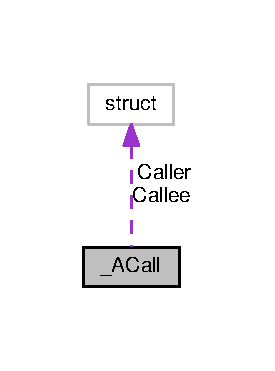
\includegraphics[width=132pt]{struct___a_call__coll__graph}
\end{center}
\end{figure}
\subsection*{Data Fields}
\begin{DoxyCompactItemize}
\item 
\hypertarget{struct___a_call_a3a5ba243b3ab4b6093afb178de0f9509}{pthread\+\_\+t {\bfseries tid}}\label{struct___a_call_a3a5ba243b3ab4b6093afb178de0f9509}

\item 
\hypertarget{struct___a_call_ae40354a1051342eb5a9db005715dcfa9}{int {\bfseries idx}}\label{struct___a_call_ae40354a1051342eb5a9db005715dcfa9}

\item 
\hypertarget{struct___a_call_a51f82344f432ea82fc1a993d1f9cb018}{\hyperlink{struct___party}{Party} {\bfseries Caller}}\label{struct___a_call_a51f82344f432ea82fc1a993d1f9cb018}

\item 
\hypertarget{struct___a_call_ac9f376aa53c5e8c50a3ebd11c377f0dd}{\hyperlink{struct___party}{Party} {\bfseries Callee}}\label{struct___a_call_ac9f376aa53c5e8c50a3ebd11c377f0dd}

\end{DoxyCompactItemize}


\subsection{Detailed Description}


Definition at line 47 of file toxav\+\_\+many\+\_\+test.\+c.



The documentation for this struct was generated from the following file\+:\begin{DoxyCompactItemize}
\item 
auto\+\_\+tests/toxav\+\_\+many\+\_\+test.\+c\end{DoxyCompactItemize}

\hypertarget{struct___c_s_session}{\section{\+\_\+\+C\+S\+Session Struct Reference}
\label{struct___c_s_session}\index{\+\_\+\+C\+S\+Session@{\+\_\+\+C\+S\+Session}}
}


{\ttfamily \#include $<$codec.\+h$>$}



Collaboration diagram for \+\_\+\+C\+S\+Session\+:
\nopagebreak
\begin{figure}[H]
\begin{center}
\leavevmode
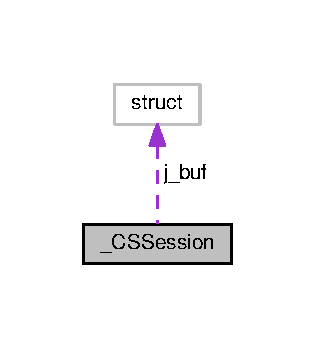
\includegraphics[width=151pt]{struct___c_s_session__coll__graph}
\end{center}
\end{figure}
\subsection*{Public Member Functions}
\begin{DoxyCompactItemize}
\item 
\hypertarget{struct___c_s_session_a386fcae0e3f3ef0fcd8b2c401a7a25e5}{{\bfseries P\+A\+I\+R} (C\+S\+Audio\+Callback, void $\ast$) acb}\label{struct___c_s_session_a386fcae0e3f3ef0fcd8b2c401a7a25e5}

\item 
\hypertarget{struct___c_s_session_a68cfb40772f235c4c4649ca156cea307}{{\bfseries P\+A\+I\+R} (C\+S\+Video\+Callback, void $\ast$) vcb}\label{struct___c_s_session_a68cfb40772f235c4c4649ca156cea307}

\end{DoxyCompactItemize}
\subsection*{Data Fields}
\begin{DoxyCompactItemize}
\item 
\hypertarget{struct___c_s_session_a269c7451109b710b39367a8ef63afce9}{int {\bfseries support\+\_\+video}}\label{struct___c_s_session_a269c7451109b710b39367a8ef63afce9}

\item 
\hypertarget{struct___c_s_session_a0ec480a7314c0f185ae18f411d73b1bd}{vpx\+\_\+codec\+\_\+ctx\+\_\+t {\bfseries v\+\_\+encoder}}\label{struct___c_s_session_a0ec480a7314c0f185ae18f411d73b1bd}

\item 
\hypertarget{struct___c_s_session_abeaee952422869c026bab7d7f3f0f145}{uint32\+\_\+t {\bfseries frame\+\_\+counter}}\label{struct___c_s_session_abeaee952422869c026bab7d7f3f0f145}

\item 
\hypertarget{struct___c_s_session_aa155f92243013193ef3fd9fd1b919bd0}{vpx\+\_\+codec\+\_\+ctx\+\_\+t {\bfseries v\+\_\+decoder}}\label{struct___c_s_session_aa155f92243013193ef3fd9fd1b919bd0}

\item 
\hypertarget{struct___c_s_session_aa224a991c08c1d696a040a415d6a4a92}{int {\bfseries max\+\_\+width}}\label{struct___c_s_session_aa224a991c08c1d696a040a415d6a4a92}

\item 
\hypertarget{struct___c_s_session_a3826471ddaa71d2730a6930625867bc1}{int {\bfseries max\+\_\+height}}\label{struct___c_s_session_a3826471ddaa71d2730a6930625867bc1}

\item 
\hypertarget{struct___c_s_session_acafa0ba061c3e09d3f17852abf830968}{unsigned int {\bfseries video\+\_\+bitrate}}\label{struct___c_s_session_acafa0ba061c3e09d3f17852abf830968}

\item 
\hypertarget{struct___c_s_session_aa4046ccf60d85f4f486ae0b24e3347f5}{uint8\+\_\+t $\ast$ {\bfseries frame\+\_\+buf}}\label{struct___c_s_session_aa4046ccf60d85f4f486ae0b24e3347f5}

\item 
\hypertarget{struct___c_s_session_a0229abcfe4414f86dcf52c5ebf84311c}{uint32\+\_\+t {\bfseries frame\+\_\+size}}\label{struct___c_s_session_a0229abcfe4414f86dcf52c5ebf84311c}

\item 
\hypertarget{struct___c_s_session_affc5ab5608c4d2dea8513fdc2b2cd6e6}{uint8\+\_\+t {\bfseries frameid\+\_\+in}}\label{struct___c_s_session_affc5ab5608c4d2dea8513fdc2b2cd6e6}

\item 
\hypertarget{struct___c_s_session_acea7b9bf7e58ed8e24980edeaacecc25}{uint8\+\_\+t {\bfseries frameid\+\_\+out}}\label{struct___c_s_session_acea7b9bf7e58ed8e24980edeaacecc25}

\item 
\hypertarget{struct___c_s_session_ab3eadf01045769905278f1908af23558}{uint32\+\_\+t {\bfseries last\+\_\+timestamp}}\label{struct___c_s_session_ab3eadf01045769905278f1908af23558}

\item 
\hypertarget{struct___c_s_session_af3563a0a96eb120a68e82d3135b6c49b}{uint32\+\_\+t {\bfseries video\+\_\+frame\+\_\+piece\+\_\+size}}\label{struct___c_s_session_af3563a0a96eb120a68e82d3135b6c49b}

\item 
\hypertarget{struct___c_s_session_a4de5a61c775468baabb35e2fcfaaa3a2}{uint32\+\_\+t {\bfseries max\+\_\+video\+\_\+frame\+\_\+size}}\label{struct___c_s_session_a4de5a61c775468baabb35e2fcfaaa3a2}

\item 
\hypertarget{struct___c_s_session_a100e5e445d6e9ff7775a1020dc780e56}{uint8\+\_\+t $\ast$ {\bfseries split\+\_\+video\+\_\+frame}}\label{struct___c_s_session_a100e5e445d6e9ff7775a1020dc780e56}

\item 
\hypertarget{struct___c_s_session_ae94ea43be63edb42efe44edae585064e}{const uint8\+\_\+t $\ast$ {\bfseries processing\+\_\+video\+\_\+frame}}\label{struct___c_s_session_ae94ea43be63edb42efe44edae585064e}

\item 
\hypertarget{struct___c_s_session_a7048faa402d6aecd2626ed85f352f5f2}{uint16\+\_\+t {\bfseries processing\+\_\+video\+\_\+frame\+\_\+size}}\label{struct___c_s_session_a7048faa402d6aecd2626ed85f352f5f2}

\item 
\hypertarget{struct___c_s_session_a8c1fa3d73f3426ba5cac83857c390ebc}{Opus\+Encoder $\ast$ {\bfseries audio\+\_\+encoder}}\label{struct___c_s_session_a8c1fa3d73f3426ba5cac83857c390ebc}

\item 
\hypertarget{struct___c_s_session_a8951572b99eec737269f5de96f9c5320}{int {\bfseries audio\+\_\+encoder\+\_\+bitrate}}\label{struct___c_s_session_a8951572b99eec737269f5de96f9c5320}

\item 
\hypertarget{struct___c_s_session_ae40829dc4300d79d3b175c8770b769a4}{int {\bfseries audio\+\_\+encoder\+\_\+sample\+\_\+rate}}\label{struct___c_s_session_ae40829dc4300d79d3b175c8770b769a4}

\item 
\hypertarget{struct___c_s_session_a25f8c6ef812a7edaaadb81b41f8d818d}{int {\bfseries audio\+\_\+encoder\+\_\+frame\+\_\+duration}}\label{struct___c_s_session_a25f8c6ef812a7edaaadb81b41f8d818d}

\item 
\hypertarget{struct___c_s_session_a8ee56e2e7543722415f21dcc3ace1899}{int {\bfseries audio\+\_\+encoder\+\_\+channels}}\label{struct___c_s_session_a8ee56e2e7543722415f21dcc3ace1899}

\item 
\hypertarget{struct___c_s_session_a3b9ee5ac4c354a3e31a8acf7aa1a1b6c}{Opus\+Decoder $\ast$ {\bfseries audio\+\_\+decoder}}\label{struct___c_s_session_a3b9ee5ac4c354a3e31a8acf7aa1a1b6c}

\item 
\hypertarget{struct___c_s_session_a56e0bd5af866e6ba91078960083ac801}{int {\bfseries audio\+\_\+decoder\+\_\+bitrate}}\label{struct___c_s_session_a56e0bd5af866e6ba91078960083ac801}

\item 
\hypertarget{struct___c_s_session_a22979ca479f4d3e2660b604805a41833}{int {\bfseries audio\+\_\+decoder\+\_\+sample\+\_\+rate}}\label{struct___c_s_session_a22979ca479f4d3e2660b604805a41833}

\item 
\hypertarget{struct___c_s_session_a245af4e824b82e6e91850ac26ace1230}{int {\bfseries audio\+\_\+decoder\+\_\+frame\+\_\+duration}}\label{struct___c_s_session_a245af4e824b82e6e91850ac26ace1230}

\item 
\hypertarget{struct___c_s_session_a81fe9534366c7ea81e8ff6ac729d2ae9}{int {\bfseries audio\+\_\+decoder\+\_\+channels}}\label{struct___c_s_session_a81fe9534366c7ea81e8ff6ac729d2ae9}

\item 
\hypertarget{struct___c_s_session_a7567f0c621b65df3ff9e6f46164ac1c0}{struct \hyperlink{struct___jitter_buffer}{\+\_\+\+Jitter\+Buffer} $\ast$ {\bfseries j\+\_\+buf}}\label{struct___c_s_session_a7567f0c621b65df3ff9e6f46164ac1c0}

\item 
\hypertarget{struct___c_s_session_a7d48e69ed8663d4dbe8266ff4158a321}{uint32\+\_\+t {\bfseries E\+V\+A\+D\+\_\+tolerance}}\label{struct___c_s_session_a7d48e69ed8663d4dbe8266ff4158a321}

\item 
\hypertarget{struct___c_s_session_aa799246d78fac3297846637588131763}{uint32\+\_\+t {\bfseries E\+V\+A\+D\+\_\+tolerance\+\_\+cr}}\label{struct___c_s_session_aa799246d78fac3297846637588131763}

\item 
\hypertarget{struct___c_s_session_ac9e675ead9b3559ea462414a0016f6a6}{uint64\+\_\+t {\bfseries capabilities}}\label{struct___c_s_session_ac9e675ead9b3559ea462414a0016f6a6}

\item 
\hypertarget{struct___c_s_session_abb525d3cf1486064b35b5821a0646c86}{void $\ast$ {\bfseries vbuf\+\_\+raw}}\label{struct___c_s_session_abb525d3cf1486064b35b5821a0646c86}

\item 
\hypertarget{struct___c_s_session_aa1e20c410f3ec23066afb256fa3d1254}{pthread\+\_\+mutex\+\_\+t {\bfseries queue\+\_\+mutex} \mbox{[}1\mbox{]}}\label{struct___c_s_session_aa1e20c410f3ec23066afb256fa3d1254}

\item 
\hypertarget{struct___c_s_session_a18e94ace0074984593ae281f6bbda315}{void $\ast$ {\bfseries agent}}\label{struct___c_s_session_a18e94ace0074984593ae281f6bbda315}

\item 
\hypertarget{struct___c_s_session_ad6b287fd08a0cc466cd41bd2e76d5808}{int32\+\_\+t {\bfseries call\+\_\+idx}}\label{struct___c_s_session_ad6b287fd08a0cc466cd41bd2e76d5808}

\end{DoxyCompactItemize}


\subsection{Detailed Description}
Codec session -\/ controling codec 

Definition at line 72 of file codec.\+h.



The documentation for this struct was generated from the following file\+:\begin{DoxyCompactItemize}
\item 
toxav/codec.\+h\end{DoxyCompactItemize}

\hypertarget{struct___jitter_buffer}{\section{\+\_\+\+Jitter\+Buffer Struct Reference}
\label{struct___jitter_buffer}\index{\+\_\+\+Jitter\+Buffer@{\+\_\+\+Jitter\+Buffer}}
}


Collaboration diagram for \+\_\+\+Jitter\+Buffer\+:
\nopagebreak
\begin{figure}[H]
\begin{center}
\leavevmode
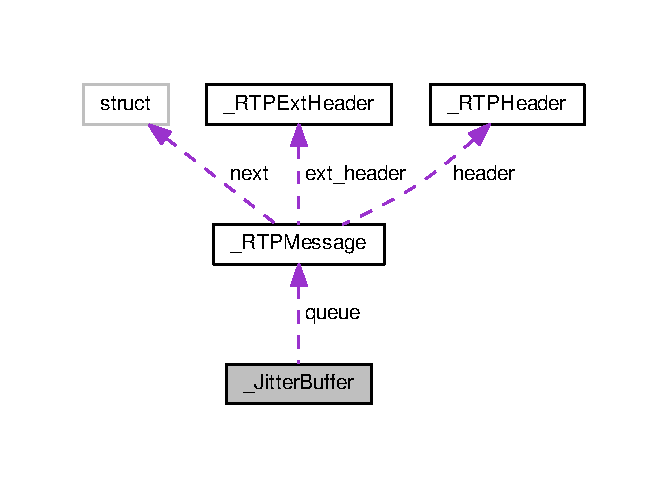
\includegraphics[width=321pt]{d1/d88/struct___jitter_buffer__coll__graph}
\end{center}
\end{figure}
\subsection*{Data Fields}
\begin{DoxyCompactItemize}
\item 
\hyperlink{rtp_8h_ab98525fe7a493c34d9dc586aa5b029b6}{R\+T\+P\+Message} $\ast$$\ast$ \hyperlink{struct___jitter_buffer_aba0e7057fa735d7bfaa585fd7bf43a24}{queue}
\item 
uint32\+\_\+t \hyperlink{struct___jitter_buffer_ab2c6b258f02add8fdf4cfc7c371dd772}{size}
\item 
uint32\+\_\+t \hyperlink{struct___jitter_buffer_a391c992c66c3e5540265a85ec2b9216a}{capacity}
\item 
uint16\+\_\+t \hyperlink{struct___jitter_buffer_a12c8099ac87952580dd090215e02728c}{bottom}
\item 
uint16\+\_\+t \hyperlink{struct___jitter_buffer_a0c235a6df98714bb18538fc0afc5bad1}{top}
\end{DoxyCompactItemize}


\subsection{Detailed Description}


Definition at line 123 of file codec.\+c.



\subsection{Field Documentation}
\hypertarget{struct___jitter_buffer_a12c8099ac87952580dd090215e02728c}{\index{\+\_\+\+Jitter\+Buffer@{\+\_\+\+Jitter\+Buffer}!bottom@{bottom}}
\index{bottom@{bottom}!\+\_\+\+Jitter\+Buffer@{\+\_\+\+Jitter\+Buffer}}
\subsubsection[{bottom}]{\setlength{\rightskip}{0pt plus 5cm}uint16\+\_\+t bottom}}\label{struct___jitter_buffer_a12c8099ac87952580dd090215e02728c}


Definition at line 127 of file codec.\+c.



Referenced by jbuf\+\_\+clear(), jbuf\+\_\+read(), and jbuf\+\_\+write().

\hypertarget{struct___jitter_buffer_a391c992c66c3e5540265a85ec2b9216a}{\index{\+\_\+\+Jitter\+Buffer@{\+\_\+\+Jitter\+Buffer}!capacity@{capacity}}
\index{capacity@{capacity}!\+\_\+\+Jitter\+Buffer@{\+\_\+\+Jitter\+Buffer}}
\subsubsection[{capacity}]{\setlength{\rightskip}{0pt plus 5cm}uint32\+\_\+t capacity}}\label{struct___jitter_buffer_a391c992c66c3e5540265a85ec2b9216a}


Definition at line 126 of file codec.\+c.



Referenced by jbuf\+\_\+new(), jbuf\+\_\+read(), and jbuf\+\_\+write().

\hypertarget{struct___jitter_buffer_aba0e7057fa735d7bfaa585fd7bf43a24}{\index{\+\_\+\+Jitter\+Buffer@{\+\_\+\+Jitter\+Buffer}!queue@{queue}}
\index{queue@{queue}!\+\_\+\+Jitter\+Buffer@{\+\_\+\+Jitter\+Buffer}}
\subsubsection[{queue}]{\setlength{\rightskip}{0pt plus 5cm}{\bf R\+T\+P\+Message}$\ast$$\ast$ queue}}\label{struct___jitter_buffer_aba0e7057fa735d7bfaa585fd7bf43a24}


Definition at line 124 of file codec.\+c.



Referenced by jbuf\+\_\+clear(), jbuf\+\_\+free(), jbuf\+\_\+new(), jbuf\+\_\+read(), and jbuf\+\_\+write().

\hypertarget{struct___jitter_buffer_ab2c6b258f02add8fdf4cfc7c371dd772}{\index{\+\_\+\+Jitter\+Buffer@{\+\_\+\+Jitter\+Buffer}!size@{size}}
\index{size@{size}!\+\_\+\+Jitter\+Buffer@{\+\_\+\+Jitter\+Buffer}}
\subsubsection[{size}]{\setlength{\rightskip}{0pt plus 5cm}uint32\+\_\+t size}}\label{struct___jitter_buffer_ab2c6b258f02add8fdf4cfc7c371dd772}


Definition at line 125 of file codec.\+c.



Referenced by jbuf\+\_\+clear(), jbuf\+\_\+new(), jbuf\+\_\+read(), and jbuf\+\_\+write().

\hypertarget{struct___jitter_buffer_a0c235a6df98714bb18538fc0afc5bad1}{\index{\+\_\+\+Jitter\+Buffer@{\+\_\+\+Jitter\+Buffer}!top@{top}}
\index{top@{top}!\+\_\+\+Jitter\+Buffer@{\+\_\+\+Jitter\+Buffer}}
\subsubsection[{top}]{\setlength{\rightskip}{0pt plus 5cm}uint16\+\_\+t top}}\label{struct___jitter_buffer_a0c235a6df98714bb18538fc0afc5bad1}


Definition at line 128 of file codec.\+c.



Referenced by jbuf\+\_\+clear(), jbuf\+\_\+read(), and jbuf\+\_\+write().



The documentation for this struct was generated from the following file\+:\begin{DoxyCompactItemize}
\item 
toxav/\hyperlink{codec_8c}{codec.\+c}\end{DoxyCompactItemize}

\hypertarget{struct___m_s_i_call}{\section{\+\_\+\+M\+S\+I\+Call Struct Reference}
\label{struct___m_s_i_call}\index{\+\_\+\+M\+S\+I\+Call@{\+\_\+\+M\+S\+I\+Call}}
}


{\ttfamily \#include $<$msi.\+h$>$}



Collaboration diagram for \+\_\+\+M\+S\+I\+Call\+:
\nopagebreak
\begin{figure}[H]
\begin{center}
\leavevmode
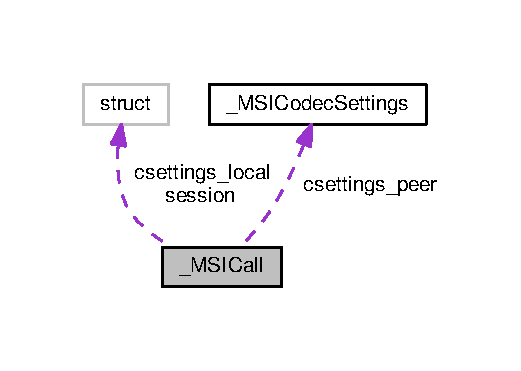
\includegraphics[width=250pt]{d5/d5b/struct___m_s_i_call__coll__graph}
\end{center}
\end{figure}
\subsection*{Data Fields}
\begin{DoxyCompactItemize}
\item 
struct \hyperlink{struct___m_s_i_session}{\+\_\+\+M\+S\+I\+Session} $\ast$ \hyperlink{struct___m_s_i_call_ab8c2a41964c26c7f08f62fa440541b12}{session}
\item 
\hyperlink{msi_8h_afbc789bbdb9a4d00eda005500f7c1675}{M\+S\+I\+Call\+State} \hyperlink{struct___m_s_i_call_a4a1fc0e5d23dbdc357786d4c69eda9b9}{state}
\item 
\hyperlink{msi_8h_abe548d26a24458ebf9ab33310ee19600}{M\+S\+I\+C\+Settings} \hyperlink{struct___m_s_i_call_ae57cfc81fffd82f53953c6546bb9f3c3}{csettings\+\_\+local}
\item 
\hyperlink{msi_8h_abe548d26a24458ebf9ab33310ee19600}{M\+S\+I\+C\+Settings} $\ast$ \hyperlink{struct___m_s_i_call_a3b7fc70c2772bbdc453eeff763fc0b4c}{csettings\+\_\+peer}
\item 
\hyperlink{msi_8h_a861af5c5c180987c1c86739b4321076c}{M\+S\+I\+Call\+I\+D\+Type} \hyperlink{struct___m_s_i_call_aa135fbffd11268758f5f21269fb46853}{id}
\item 
int \hyperlink{struct___m_s_i_call_ad8fefcfbba597fbff4216644f2872acf}{ringing\+\_\+tout\+\_\+ms}
\item 
int \hyperlink{struct___m_s_i_call_a8ccfd1cd9f807007763f41eafd801130}{request\+\_\+timer\+\_\+id}
\item 
int \hyperlink{struct___m_s_i_call_a94fdc66dbd509ba4e89edcedb8e11022}{ringing\+\_\+timer\+\_\+id}
\item 
uint32\+\_\+t $\ast$ \hyperlink{struct___m_s_i_call_a55d2568491d616f7fef07bc7137c8c23}{peers}
\item 
uint16\+\_\+t \hyperlink{struct___m_s_i_call_a62e9da1e57f84fd224590c4d466724aa}{peer\+\_\+count}
\item 
int32\+\_\+t \hyperlink{struct___m_s_i_call_ad6b287fd08a0cc466cd41bd2e76d5808}{call\+\_\+idx}
\end{DoxyCompactItemize}


\subsection{Detailed Description}
The call struct. 

Definition at line 100 of file msi.\+h.



\subsection{Field Documentation}
\hypertarget{struct___m_s_i_call_ad6b287fd08a0cc466cd41bd2e76d5808}{\index{\+\_\+\+M\+S\+I\+Call@{\+\_\+\+M\+S\+I\+Call}!call\+\_\+idx@{call\+\_\+idx}}
\index{call\+\_\+idx@{call\+\_\+idx}!\+\_\+\+M\+S\+I\+Call@{\+\_\+\+M\+S\+I\+Call}}
\subsubsection[{call\+\_\+idx}]{\setlength{\rightskip}{0pt plus 5cm}int32\+\_\+t call\+\_\+idx}}\label{struct___m_s_i_call_ad6b287fd08a0cc466cd41bd2e76d5808}


Definition at line 118 of file msi.\+h.



Referenced by handle\+\_\+recv\+\_\+cancel(), handle\+\_\+recv\+\_\+end(), handle\+\_\+recv\+\_\+ending(), handle\+\_\+recv\+\_\+error(), handle\+\_\+recv\+\_\+invite(), handle\+\_\+recv\+\_\+reject(), handle\+\_\+recv\+\_\+ringing(), handle\+\_\+recv\+\_\+start(), handle\+\_\+recv\+\_\+starting(), handle\+\_\+timeout(), init\+\_\+call(), msi\+\_\+invite(), and terminate\+\_\+call().

\hypertarget{struct___m_s_i_call_ae57cfc81fffd82f53953c6546bb9f3c3}{\index{\+\_\+\+M\+S\+I\+Call@{\+\_\+\+M\+S\+I\+Call}!csettings\+\_\+local@{csettings\+\_\+local}}
\index{csettings\+\_\+local@{csettings\+\_\+local}!\+\_\+\+M\+S\+I\+Call@{\+\_\+\+M\+S\+I\+Call}}
\subsubsection[{csettings\+\_\+local}]{\setlength{\rightskip}{0pt plus 5cm}{\bf M\+S\+I\+C\+Settings} csettings\+\_\+local}}\label{struct___m_s_i_call_ae57cfc81fffd82f53953c6546bb9f3c3}


Definition at line 105 of file msi.\+h.



Referenced by msi\+\_\+answer(), msi\+\_\+change\+\_\+csettings(), msi\+\_\+invite(), and toxav\+\_\+prepare\+\_\+transmission().

\hypertarget{struct___m_s_i_call_a3b7fc70c2772bbdc453eeff763fc0b4c}{\index{\+\_\+\+M\+S\+I\+Call@{\+\_\+\+M\+S\+I\+Call}!csettings\+\_\+peer@{csettings\+\_\+peer}}
\index{csettings\+\_\+peer@{csettings\+\_\+peer}!\+\_\+\+M\+S\+I\+Call@{\+\_\+\+M\+S\+I\+Call}}
\subsubsection[{csettings\+\_\+peer}]{\setlength{\rightskip}{0pt plus 5cm}{\bf M\+S\+I\+C\+Settings}$\ast$ csettings\+\_\+peer}}\label{struct___m_s_i_call_a3b7fc70c2772bbdc453eeff763fc0b4c}


Definition at line 106 of file msi.\+h.



Referenced by flush\+\_\+peer\+\_\+csettings(), handle\+\_\+recv\+\_\+invite(), init\+\_\+call(), terminate\+\_\+call(), toxav\+\_\+get\+\_\+peer\+\_\+csettings(), and toxav\+\_\+prepare\+\_\+transmission().

\hypertarget{struct___m_s_i_call_aa135fbffd11268758f5f21269fb46853}{\index{\+\_\+\+M\+S\+I\+Call@{\+\_\+\+M\+S\+I\+Call}!id@{id}}
\index{id@{id}!\+\_\+\+M\+S\+I\+Call@{\+\_\+\+M\+S\+I\+Call}}
\subsubsection[{id}]{\setlength{\rightskip}{0pt plus 5cm}{\bf M\+S\+I\+Call\+I\+D\+Type} id}}\label{struct___m_s_i_call_aa135fbffd11268758f5f21269fb46853}


Definition at line 108 of file msi.\+h.



Referenced by find\+\_\+call(), handle\+\_\+recv\+\_\+invite(), msi\+\_\+invite(), send\+\_\+error(), and send\+\_\+message().

\hypertarget{struct___m_s_i_call_a62e9da1e57f84fd224590c4d466724aa}{\index{\+\_\+\+M\+S\+I\+Call@{\+\_\+\+M\+S\+I\+Call}!peer\+\_\+count@{peer\+\_\+count}}
\index{peer\+\_\+count@{peer\+\_\+count}!\+\_\+\+M\+S\+I\+Call@{\+\_\+\+M\+S\+I\+Call}}
\subsubsection[{peer\+\_\+count}]{\setlength{\rightskip}{0pt plus 5cm}uint16\+\_\+t peer\+\_\+count}}\label{struct___m_s_i_call_a62e9da1e57f84fd224590c4d466724aa}


Definition at line 116 of file msi.\+h.



Referenced by add\+\_\+peer(), handle\+\_\+remote\+\_\+connection\+\_\+change(), msi\+\_\+hangup(), msi\+\_\+reject(), toxav\+\_\+get\+\_\+peer\+\_\+csettings(), and toxav\+\_\+get\+\_\+peer\+\_\+id().

\hypertarget{struct___m_s_i_call_a55d2568491d616f7fef07bc7137c8c23}{\index{\+\_\+\+M\+S\+I\+Call@{\+\_\+\+M\+S\+I\+Call}!peers@{peers}}
\index{peers@{peers}!\+\_\+\+M\+S\+I\+Call@{\+\_\+\+M\+S\+I\+Call}}
\subsubsection[{peers}]{\setlength{\rightskip}{0pt plus 5cm}uint32\+\_\+t$\ast$ peers}}\label{struct___m_s_i_call_a55d2568491d616f7fef07bc7137c8c23}


Definition at line 115 of file msi.\+h.



Referenced by add\+\_\+peer(), handle\+\_\+recv\+\_\+invite(), handle\+\_\+remote\+\_\+connection\+\_\+change(), handle\+\_\+timeout(), msi\+\_\+answer(), msi\+\_\+change\+\_\+csettings(), msi\+\_\+hangup(), msi\+\_\+invite(), msi\+\_\+kill(), msi\+\_\+reject(), terminate\+\_\+call(), toxav\+\_\+get\+\_\+peer\+\_\+id(), and toxav\+\_\+prepare\+\_\+transmission().

\hypertarget{struct___m_s_i_call_a8ccfd1cd9f807007763f41eafd801130}{\index{\+\_\+\+M\+S\+I\+Call@{\+\_\+\+M\+S\+I\+Call}!request\+\_\+timer\+\_\+id@{request\+\_\+timer\+\_\+id}}
\index{request\+\_\+timer\+\_\+id@{request\+\_\+timer\+\_\+id}!\+\_\+\+M\+S\+I\+Call@{\+\_\+\+M\+S\+I\+Call}}
\subsubsection[{request\+\_\+timer\+\_\+id}]{\setlength{\rightskip}{0pt plus 5cm}int request\+\_\+timer\+\_\+id}}\label{struct___m_s_i_call_a8ccfd1cd9f807007763f41eafd801130}


Definition at line 112 of file msi.\+h.



Referenced by init\+\_\+call(), msi\+\_\+handle\+\_\+packet(), msi\+\_\+hangup(), msi\+\_\+invite(), msi\+\_\+reject(), and terminate\+\_\+call().

\hypertarget{struct___m_s_i_call_a94fdc66dbd509ba4e89edcedb8e11022}{\index{\+\_\+\+M\+S\+I\+Call@{\+\_\+\+M\+S\+I\+Call}!ringing\+\_\+timer\+\_\+id@{ringing\+\_\+timer\+\_\+id}}
\index{ringing\+\_\+timer\+\_\+id@{ringing\+\_\+timer\+\_\+id}!\+\_\+\+M\+S\+I\+Call@{\+\_\+\+M\+S\+I\+Call}}
\subsubsection[{ringing\+\_\+timer\+\_\+id}]{\setlength{\rightskip}{0pt plus 5cm}int ringing\+\_\+timer\+\_\+id}}\label{struct___m_s_i_call_a94fdc66dbd509ba4e89edcedb8e11022}


Definition at line 113 of file msi.\+h.



Referenced by handle\+\_\+recv\+\_\+ringing(), handle\+\_\+recv\+\_\+starting(), init\+\_\+call(), and terminate\+\_\+call().

\hypertarget{struct___m_s_i_call_ad8fefcfbba597fbff4216644f2872acf}{\index{\+\_\+\+M\+S\+I\+Call@{\+\_\+\+M\+S\+I\+Call}!ringing\+\_\+tout\+\_\+ms@{ringing\+\_\+tout\+\_\+ms}}
\index{ringing\+\_\+tout\+\_\+ms@{ringing\+\_\+tout\+\_\+ms}!\+\_\+\+M\+S\+I\+Call@{\+\_\+\+M\+S\+I\+Call}}
\subsubsection[{ringing\+\_\+tout\+\_\+ms}]{\setlength{\rightskip}{0pt plus 5cm}int ringing\+\_\+tout\+\_\+ms}}\label{struct___m_s_i_call_ad8fefcfbba597fbff4216644f2872acf}


Definition at line 110 of file msi.\+h.



Referenced by handle\+\_\+recv\+\_\+ringing(), and init\+\_\+call().

\hypertarget{struct___m_s_i_call_ab8c2a41964c26c7f08f62fa440541b12}{\index{\+\_\+\+M\+S\+I\+Call@{\+\_\+\+M\+S\+I\+Call}!session@{session}}
\index{session@{session}!\+\_\+\+M\+S\+I\+Call@{\+\_\+\+M\+S\+I\+Call}}
\subsubsection[{session}]{\setlength{\rightskip}{0pt plus 5cm}struct {\bf \+\_\+\+M\+S\+I\+Session}$\ast$ session}}\label{struct___m_s_i_call_ab8c2a41964c26c7f08f62fa440541b12}


Definition at line 101 of file msi.\+h.



Referenced by init\+\_\+call().

\hypertarget{struct___m_s_i_call_a4a1fc0e5d23dbdc357786d4c69eda9b9}{\index{\+\_\+\+M\+S\+I\+Call@{\+\_\+\+M\+S\+I\+Call}!state@{state}}
\index{state@{state}!\+\_\+\+M\+S\+I\+Call@{\+\_\+\+M\+S\+I\+Call}}
\subsubsection[{state}]{\setlength{\rightskip}{0pt plus 5cm}{\bf M\+S\+I\+Call\+State} state}}\label{struct___m_s_i_call_a4a1fc0e5d23dbdc357786d4c69eda9b9}


Definition at line 103 of file msi.\+h.



Referenced by handle\+\_\+recv\+\_\+invite(), handle\+\_\+recv\+\_\+start(), handle\+\_\+recv\+\_\+starting(), msi\+\_\+answer(), msi\+\_\+cancel(), msi\+\_\+change\+\_\+csettings(), msi\+\_\+hangup(), msi\+\_\+invite(), msi\+\_\+kill(), msi\+\_\+reject(), and toxav\+\_\+get\+\_\+call\+\_\+state().



The documentation for this struct was generated from the following file\+:\begin{DoxyCompactItemize}
\item 
toxav/\hyperlink{msi_8h}{msi.\+h}\end{DoxyCompactItemize}

\hypertarget{struct___m_s_i_codec_settings}{\section{\+\_\+\+M\+S\+I\+Codec\+Settings Struct Reference}
\label{struct___m_s_i_codec_settings}\index{\+\_\+\+M\+S\+I\+Codec\+Settings@{\+\_\+\+M\+S\+I\+Codec\+Settings}}
}


{\ttfamily \#include $<$msi.\+h$>$}

\subsection*{Data Fields}
\begin{DoxyCompactItemize}
\item 
\hyperlink{msi_8h_a54df3a97d8d112a3a4a6476c9f9284a6}{M\+S\+I\+Call\+Type} \hyperlink{struct___m_s_i_codec_settings_a24d841d0ab8a0b3f12f559aec494e4fe}{call\+\_\+type}
\item 
uint32\+\_\+t \hyperlink{struct___m_s_i_codec_settings_af0eac99d4181795e8a595d244e745192}{video\+\_\+bitrate}
\item 
uint16\+\_\+t \hyperlink{struct___m_s_i_codec_settings_ab81ecded1f7c46e120c8f2afa7b2c5cc}{max\+\_\+video\+\_\+width}
\item 
uint16\+\_\+t \hyperlink{struct___m_s_i_codec_settings_a4fef4b2fa1a8ae8446314ad0af4ce698}{max\+\_\+video\+\_\+height}
\item 
uint32\+\_\+t \hyperlink{struct___m_s_i_codec_settings_a5d9a8b59b2eb1eef8dbdcb032bf1dd01}{audio\+\_\+bitrate}
\item 
uint16\+\_\+t \hyperlink{struct___m_s_i_codec_settings_a61b592233f5a65705eb2600d38e365cd}{audio\+\_\+frame\+\_\+duration}
\item 
uint32\+\_\+t \hyperlink{struct___m_s_i_codec_settings_a66da4482e934a2700e07a39fa0838559}{audio\+\_\+sample\+\_\+rate}
\item 
uint32\+\_\+t \hyperlink{struct___m_s_i_codec_settings_a1b04e9669a2929f425e867440b6d826d}{audio\+\_\+channels}
\end{DoxyCompactItemize}


\subsection{Detailed Description}
Encoding settings. 

Definition at line 57 of file msi.\+h.



\subsection{Field Documentation}
\hypertarget{struct___m_s_i_codec_settings_a5d9a8b59b2eb1eef8dbdcb032bf1dd01}{\index{\+\_\+\+M\+S\+I\+Codec\+Settings@{\+\_\+\+M\+S\+I\+Codec\+Settings}!audio\+\_\+bitrate@{audio\+\_\+bitrate}}
\index{audio\+\_\+bitrate@{audio\+\_\+bitrate}!\+\_\+\+M\+S\+I\+Codec\+Settings@{\+\_\+\+M\+S\+I\+Codec\+Settings}}
\subsubsection[{audio\+\_\+bitrate}]{\setlength{\rightskip}{0pt plus 5cm}uint32\+\_\+t audio\+\_\+bitrate}}\label{struct___m_s_i_codec_settings_a5d9a8b59b2eb1eef8dbdcb032bf1dd01}


Definition at line 64 of file msi.\+h.



Referenced by flush\+\_\+peer\+\_\+csettings(), msi\+\_\+change\+\_\+csettings(), msi\+\_\+msg\+\_\+get\+\_\+csettings(), and msi\+\_\+msg\+\_\+set\+\_\+csettings().

\hypertarget{struct___m_s_i_codec_settings_a1b04e9669a2929f425e867440b6d826d}{\index{\+\_\+\+M\+S\+I\+Codec\+Settings@{\+\_\+\+M\+S\+I\+Codec\+Settings}!audio\+\_\+channels@{audio\+\_\+channels}}
\index{audio\+\_\+channels@{audio\+\_\+channels}!\+\_\+\+M\+S\+I\+Codec\+Settings@{\+\_\+\+M\+S\+I\+Codec\+Settings}}
\subsubsection[{audio\+\_\+channels}]{\setlength{\rightskip}{0pt plus 5cm}uint32\+\_\+t audio\+\_\+channels}}\label{struct___m_s_i_codec_settings_a1b04e9669a2929f425e867440b6d826d}


Definition at line 67 of file msi.\+h.



Referenced by flush\+\_\+peer\+\_\+csettings(), msi\+\_\+change\+\_\+csettings(), msi\+\_\+msg\+\_\+get\+\_\+csettings(), and msi\+\_\+msg\+\_\+set\+\_\+csettings().

\hypertarget{struct___m_s_i_codec_settings_a61b592233f5a65705eb2600d38e365cd}{\index{\+\_\+\+M\+S\+I\+Codec\+Settings@{\+\_\+\+M\+S\+I\+Codec\+Settings}!audio\+\_\+frame\+\_\+duration@{audio\+\_\+frame\+\_\+duration}}
\index{audio\+\_\+frame\+\_\+duration@{audio\+\_\+frame\+\_\+duration}!\+\_\+\+M\+S\+I\+Codec\+Settings@{\+\_\+\+M\+S\+I\+Codec\+Settings}}
\subsubsection[{audio\+\_\+frame\+\_\+duration}]{\setlength{\rightskip}{0pt plus 5cm}uint16\+\_\+t audio\+\_\+frame\+\_\+duration}}\label{struct___m_s_i_codec_settings_a61b592233f5a65705eb2600d38e365cd}


Definition at line 65 of file msi.\+h.



Referenced by flush\+\_\+peer\+\_\+csettings(), msi\+\_\+change\+\_\+csettings(), msi\+\_\+msg\+\_\+get\+\_\+csettings(), and msi\+\_\+msg\+\_\+set\+\_\+csettings().

\hypertarget{struct___m_s_i_codec_settings_a66da4482e934a2700e07a39fa0838559}{\index{\+\_\+\+M\+S\+I\+Codec\+Settings@{\+\_\+\+M\+S\+I\+Codec\+Settings}!audio\+\_\+sample\+\_\+rate@{audio\+\_\+sample\+\_\+rate}}
\index{audio\+\_\+sample\+\_\+rate@{audio\+\_\+sample\+\_\+rate}!\+\_\+\+M\+S\+I\+Codec\+Settings@{\+\_\+\+M\+S\+I\+Codec\+Settings}}
\subsubsection[{audio\+\_\+sample\+\_\+rate}]{\setlength{\rightskip}{0pt plus 5cm}uint32\+\_\+t audio\+\_\+sample\+\_\+rate}}\label{struct___m_s_i_codec_settings_a66da4482e934a2700e07a39fa0838559}


Definition at line 66 of file msi.\+h.



Referenced by flush\+\_\+peer\+\_\+csettings(), msi\+\_\+change\+\_\+csettings(), msi\+\_\+msg\+\_\+get\+\_\+csettings(), and msi\+\_\+msg\+\_\+set\+\_\+csettings().

\hypertarget{struct___m_s_i_codec_settings_a24d841d0ab8a0b3f12f559aec494e4fe}{\index{\+\_\+\+M\+S\+I\+Codec\+Settings@{\+\_\+\+M\+S\+I\+Codec\+Settings}!call\+\_\+type@{call\+\_\+type}}
\index{call\+\_\+type@{call\+\_\+type}!\+\_\+\+M\+S\+I\+Codec\+Settings@{\+\_\+\+M\+S\+I\+Codec\+Settings}}
\subsubsection[{call\+\_\+type}]{\setlength{\rightskip}{0pt plus 5cm}{\bf M\+S\+I\+Call\+Type} call\+\_\+type}}\label{struct___m_s_i_codec_settings_a24d841d0ab8a0b3f12f559aec494e4fe}


Definition at line 58 of file msi.\+h.



Referenced by flush\+\_\+peer\+\_\+csettings(), handle\+\_\+recv\+\_\+invite(), msi\+\_\+change\+\_\+csettings(), msi\+\_\+msg\+\_\+get\+\_\+csettings(), and msi\+\_\+msg\+\_\+set\+\_\+csettings().

\hypertarget{struct___m_s_i_codec_settings_a4fef4b2fa1a8ae8446314ad0af4ce698}{\index{\+\_\+\+M\+S\+I\+Codec\+Settings@{\+\_\+\+M\+S\+I\+Codec\+Settings}!max\+\_\+video\+\_\+height@{max\+\_\+video\+\_\+height}}
\index{max\+\_\+video\+\_\+height@{max\+\_\+video\+\_\+height}!\+\_\+\+M\+S\+I\+Codec\+Settings@{\+\_\+\+M\+S\+I\+Codec\+Settings}}
\subsubsection[{max\+\_\+video\+\_\+height}]{\setlength{\rightskip}{0pt plus 5cm}uint16\+\_\+t max\+\_\+video\+\_\+height}}\label{struct___m_s_i_codec_settings_a4fef4b2fa1a8ae8446314ad0af4ce698}


Definition at line 62 of file msi.\+h.



Referenced by flush\+\_\+peer\+\_\+csettings(), msi\+\_\+change\+\_\+csettings(), msi\+\_\+msg\+\_\+get\+\_\+csettings(), and msi\+\_\+msg\+\_\+set\+\_\+csettings().

\hypertarget{struct___m_s_i_codec_settings_ab81ecded1f7c46e120c8f2afa7b2c5cc}{\index{\+\_\+\+M\+S\+I\+Codec\+Settings@{\+\_\+\+M\+S\+I\+Codec\+Settings}!max\+\_\+video\+\_\+width@{max\+\_\+video\+\_\+width}}
\index{max\+\_\+video\+\_\+width@{max\+\_\+video\+\_\+width}!\+\_\+\+M\+S\+I\+Codec\+Settings@{\+\_\+\+M\+S\+I\+Codec\+Settings}}
\subsubsection[{max\+\_\+video\+\_\+width}]{\setlength{\rightskip}{0pt plus 5cm}uint16\+\_\+t max\+\_\+video\+\_\+width}}\label{struct___m_s_i_codec_settings_ab81ecded1f7c46e120c8f2afa7b2c5cc}


Definition at line 61 of file msi.\+h.



Referenced by flush\+\_\+peer\+\_\+csettings(), msi\+\_\+change\+\_\+csettings(), msi\+\_\+msg\+\_\+get\+\_\+csettings(), and msi\+\_\+msg\+\_\+set\+\_\+csettings().

\hypertarget{struct___m_s_i_codec_settings_af0eac99d4181795e8a595d244e745192}{\index{\+\_\+\+M\+S\+I\+Codec\+Settings@{\+\_\+\+M\+S\+I\+Codec\+Settings}!video\+\_\+bitrate@{video\+\_\+bitrate}}
\index{video\+\_\+bitrate@{video\+\_\+bitrate}!\+\_\+\+M\+S\+I\+Codec\+Settings@{\+\_\+\+M\+S\+I\+Codec\+Settings}}
\subsubsection[{video\+\_\+bitrate}]{\setlength{\rightskip}{0pt plus 5cm}uint32\+\_\+t video\+\_\+bitrate}}\label{struct___m_s_i_codec_settings_af0eac99d4181795e8a595d244e745192}


Definition at line 60 of file msi.\+h.



Referenced by flush\+\_\+peer\+\_\+csettings(), msi\+\_\+change\+\_\+csettings(), msi\+\_\+msg\+\_\+get\+\_\+csettings(), and msi\+\_\+msg\+\_\+set\+\_\+csettings().



The documentation for this struct was generated from the following file\+:\begin{DoxyCompactItemize}
\item 
toxav/\hyperlink{msi_8h}{msi.\+h}\end{DoxyCompactItemize}

\hypertarget{struct___m_s_i_message}{\section{\+\_\+\+M\+S\+I\+Message Struct Reference}
\label{struct___m_s_i_message}\index{\+\_\+\+M\+S\+I\+Message@{\+\_\+\+M\+S\+I\+Message}}
}
\subsection*{Data Fields}
\begin{DoxyCompactItemize}
\item 
\hypertarget{struct___m_s_i_message_a43928947ba3f33772bdeee09fd89557a}{M\+S\+I\+Header\+Request {\bfseries request}}\label{struct___m_s_i_message_a43928947ba3f33772bdeee09fd89557a}

\item 
\hypertarget{struct___m_s_i_message_a03f0f34008bf8be095af614ca99ea53f}{M\+S\+I\+Header\+Response {\bfseries response}}\label{struct___m_s_i_message_a03f0f34008bf8be095af614ca99ea53f}

\item 
\hypertarget{struct___m_s_i_message_aec4373dacf43cd56b5e67d2b04b63f5a}{M\+S\+I\+Header\+Reason {\bfseries reason}}\label{struct___m_s_i_message_aec4373dacf43cd56b5e67d2b04b63f5a}

\item 
\hypertarget{struct___m_s_i_message_a0cb3f797b633561175096933c2eb003e}{M\+S\+I\+Header\+Call\+Id {\bfseries callid}}\label{struct___m_s_i_message_a0cb3f797b633561175096933c2eb003e}

\item 
\hypertarget{struct___m_s_i_message_a4b09316f11dc8e9fe3b3357a6d48db56}{M\+S\+I\+Header\+C\+Settings {\bfseries csettings}}\label{struct___m_s_i_message_a4b09316f11dc8e9fe3b3357a6d48db56}

\item 
\hypertarget{struct___m_s_i_message_af43a034662e9bcac38e3bf4c9c150c19}{int {\bfseries friend\+\_\+id}}\label{struct___m_s_i_message_af43a034662e9bcac38e3bf4c9c150c19}

\end{DoxyCompactItemize}


\subsection{Detailed Description}


Definition at line 99 of file msi.\+c.



The documentation for this struct was generated from the following file\+:\begin{DoxyCompactItemize}
\item 
toxav/msi.\+c\end{DoxyCompactItemize}

\hypertarget{struct___m_s_i_session}{\section{\+\_\+\+M\+S\+I\+Session Struct Reference}
\label{struct___m_s_i_session}\index{\+\_\+\+M\+S\+I\+Session@{\+\_\+\+M\+S\+I\+Session}}
}


{\ttfamily \#include $<$msi.\+h$>$}



Collaboration diagram for \+\_\+\+M\+S\+I\+Session\+:
\nopagebreak
\begin{figure}[H]
\begin{center}
\leavevmode
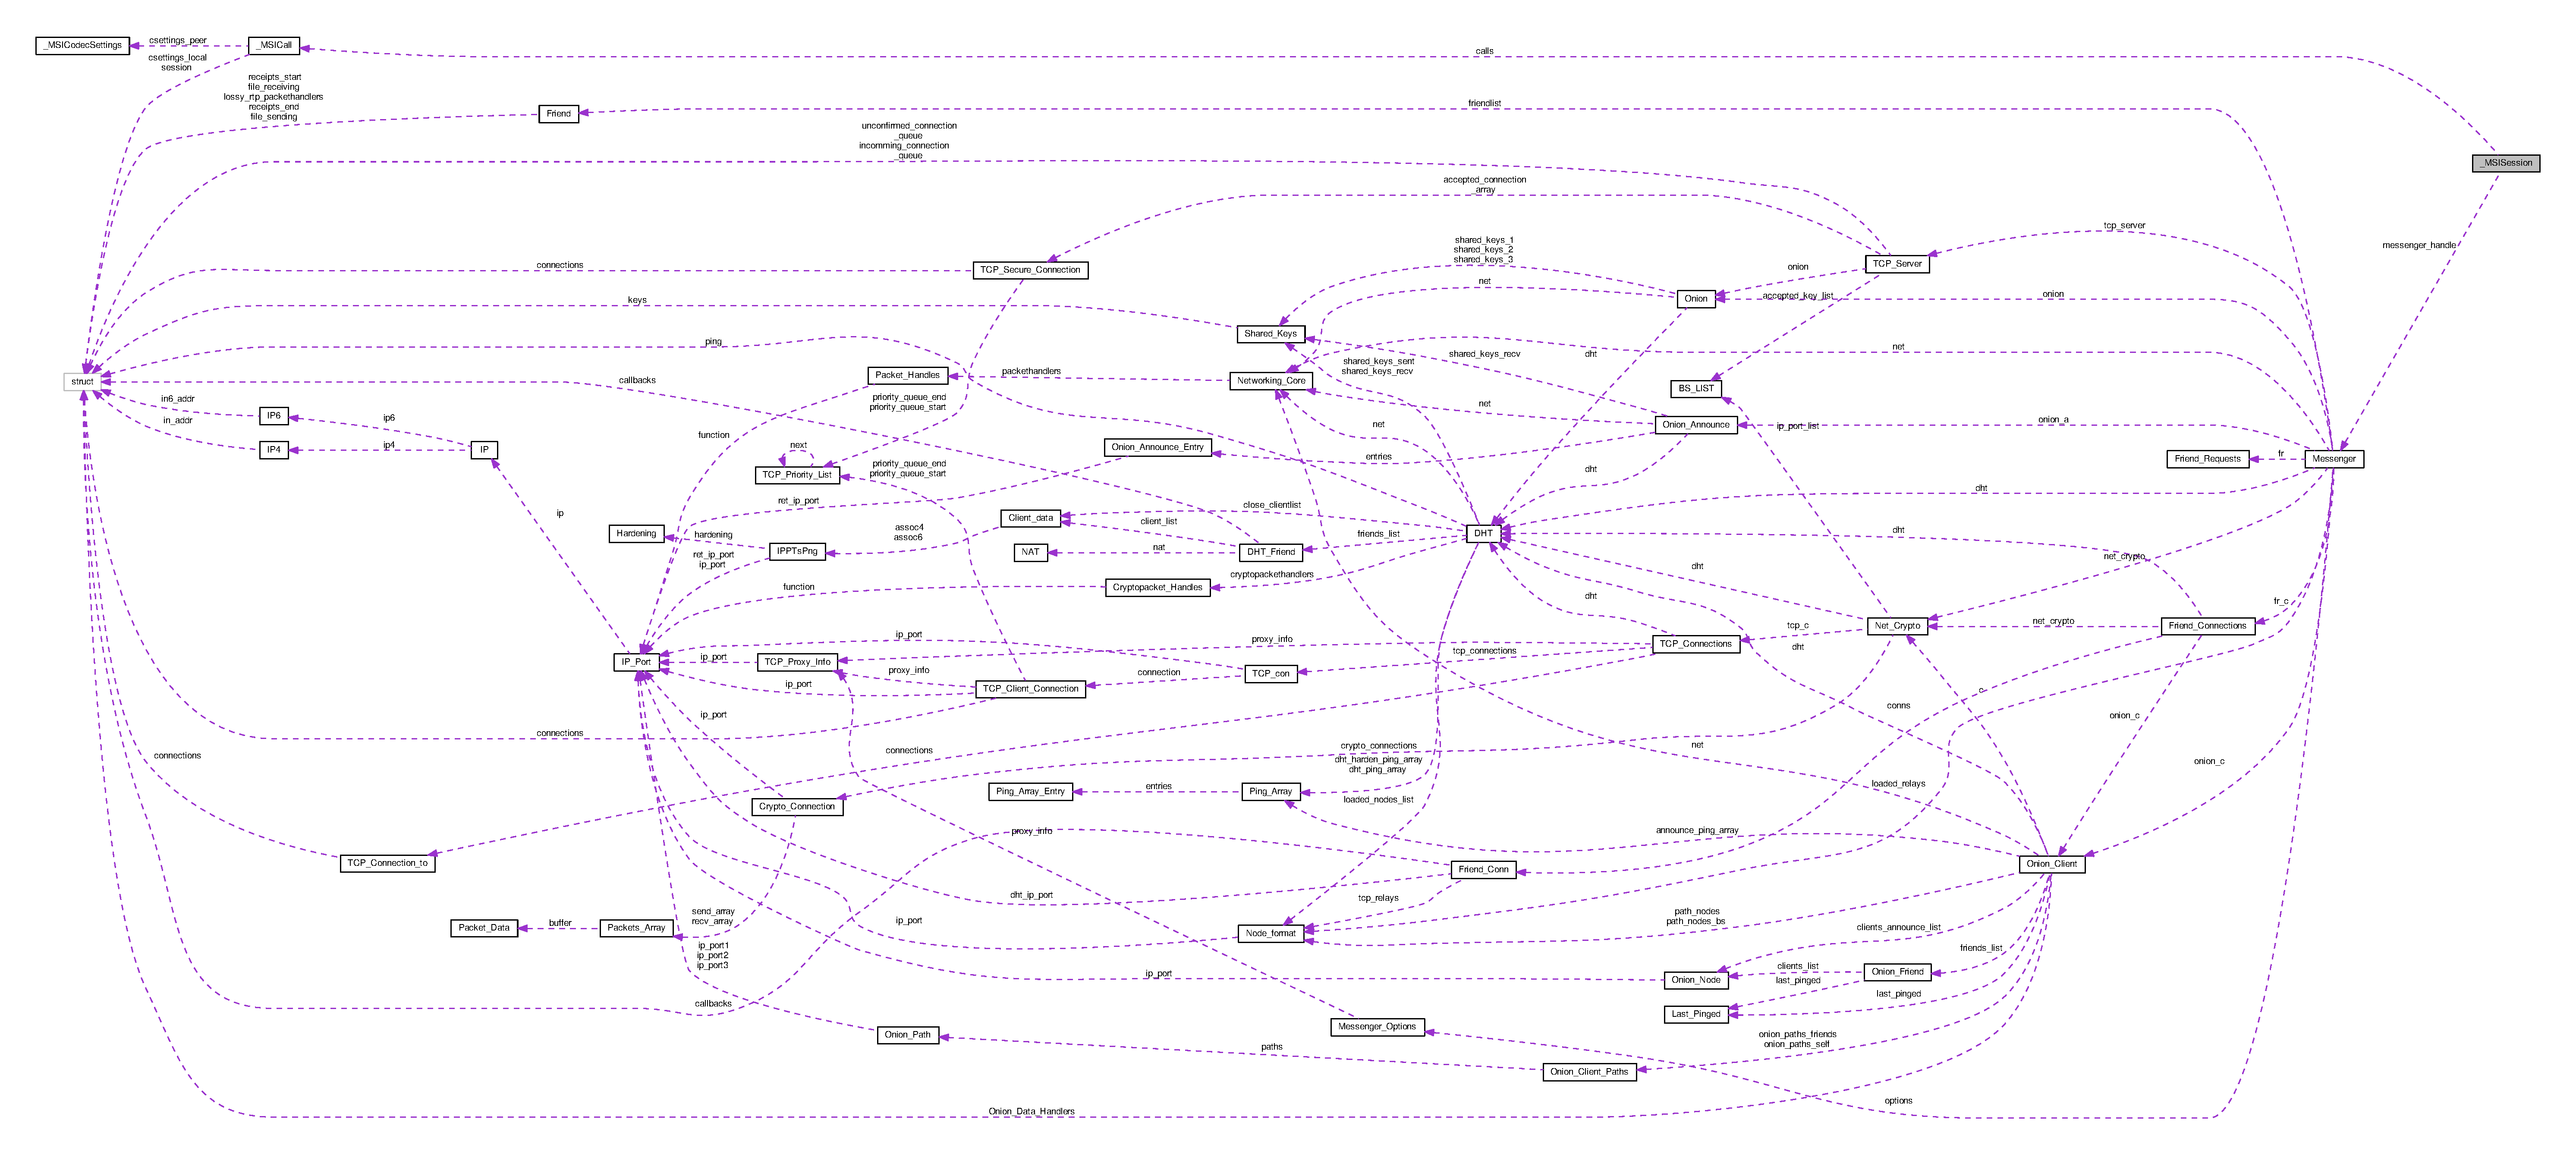
\includegraphics[width=350pt]{struct___m_s_i_session__coll__graph}
\end{center}
\end{figure}
\subsection*{Public Member Functions}
\begin{DoxyCompactItemize}
\item 
\hypertarget{struct___m_s_i_session_ad2cc3cf843c4b08a69f831cdad2eea1a}{{\bfseries P\+A\+I\+R} (M\+S\+I\+Callback\+Type, void $\ast$) callbacks\mbox{[}10\mbox{]}}\label{struct___m_s_i_session_ad2cc3cf843c4b08a69f831cdad2eea1a}

\end{DoxyCompactItemize}
\subsection*{Data Fields}
\begin{DoxyCompactItemize}
\item 
\hypertarget{struct___m_s_i_session_ac40fee673bae4030b812579c57389a02}{\hyperlink{struct___m_s_i_call}{M\+S\+I\+Call} $\ast$$\ast$ {\bfseries calls}}\label{struct___m_s_i_session_ac40fee673bae4030b812579c57389a02}

\item 
\hypertarget{struct___m_s_i_session_ae4bbb4682dc5c74588083ca06ac2f76f}{int32\+\_\+t {\bfseries max\+\_\+calls}}\label{struct___m_s_i_session_ae4bbb4682dc5c74588083ca06ac2f76f}

\item 
\hypertarget{struct___m_s_i_session_ae284478ea42e8d4ed283876c3ae18c8a}{void $\ast$ {\bfseries agent\+\_\+handler}}\label{struct___m_s_i_session_ae284478ea42e8d4ed283876c3ae18c8a}

\item 
\hypertarget{struct___m_s_i_session_a2adfe301d17504006b8321f71f642039}{\hyperlink{struct_messenger}{Messenger} $\ast$ {\bfseries messenger\+\_\+handle}}\label{struct___m_s_i_session_a2adfe301d17504006b8321f71f642039}

\item 
\hypertarget{struct___m_s_i_session_a54c9341406a254204cca6d48dd54cdc8}{uint32\+\_\+t {\bfseries frequ}}\label{struct___m_s_i_session_a54c9341406a254204cca6d48dd54cdc8}

\item 
\hypertarget{struct___m_s_i_session_a4a61d9413f442d27898849e0d8a26720}{uint32\+\_\+t {\bfseries call\+\_\+timeout}}\label{struct___m_s_i_session_a4a61d9413f442d27898849e0d8a26720}

\item 
\hypertarget{struct___m_s_i_session_ab4293016252c4d4e63549b0773fa0f33}{pthread\+\_\+mutex\+\_\+t {\bfseries mutex} \mbox{[}1\mbox{]}}\label{struct___m_s_i_session_ab4293016252c4d4e63549b0773fa0f33}

\item 
\hypertarget{struct___m_s_i_session_a06ab765308a606d809c4c2a2c71710ce}{void $\ast$ {\bfseries timer\+\_\+handler}}\label{struct___m_s_i_session_a06ab765308a606d809c4c2a2c71710ce}

\end{DoxyCompactItemize}


\subsection{Detailed Description}
Control session struct 

Definition at line 128 of file msi.\+h.



The documentation for this struct was generated from the following file\+:\begin{DoxyCompactItemize}
\item 
toxav/msi.\+h\end{DoxyCompactItemize}

\hypertarget{struct___party}{\section{\+\_\+\+Party Struct Reference}
\label{struct___party}\index{\+\_\+\+Party@{\+\_\+\+Party}}
}


Collaboration diagram for \+\_\+\+Party\+:
\nopagebreak
\begin{figure}[H]
\begin{center}
\leavevmode
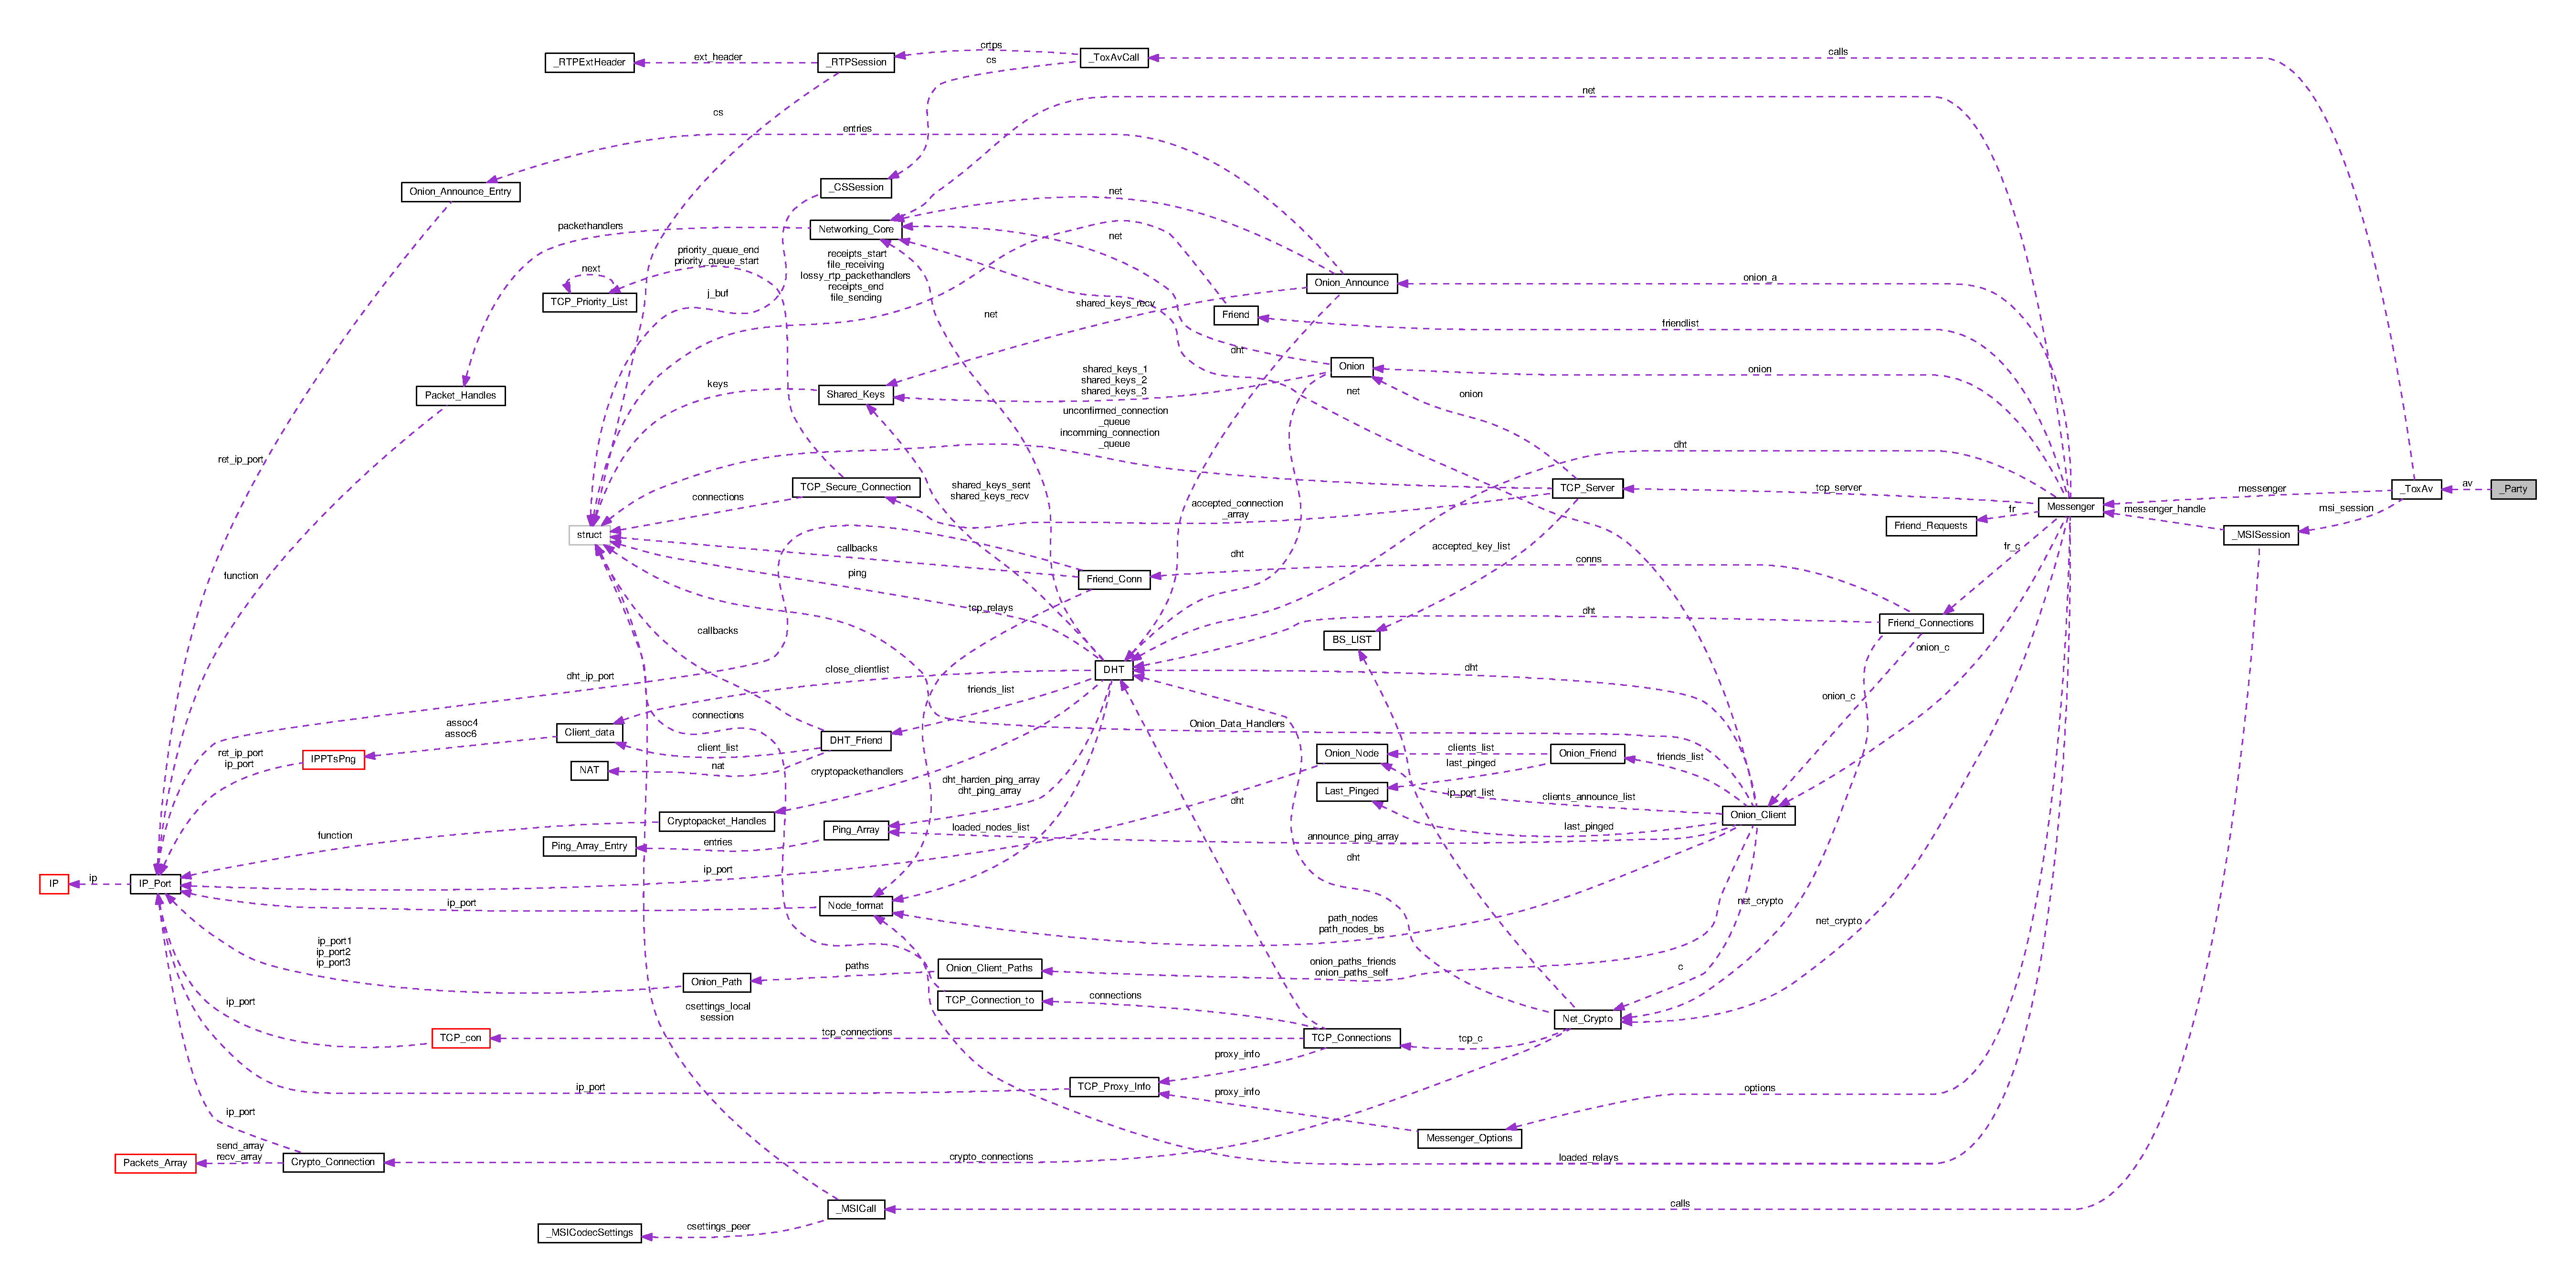
\includegraphics[width=350pt]{d2/ddc/struct___party__coll__graph}
\end{center}
\end{figure}
\subsection*{Data Fields}
\begin{DoxyCompactItemize}
\item 
\hyperlink{toxav__basic__test_8c_a377e0aa60b93038e3e9bc14c57b3d87a}{Call\+Status} \hyperlink{struct___party_a722fcd2c2e22cc6de0a53383e5871290}{status}
\item 
\hyperlink{toxav_8h_abdf4715f7de98af6ebe4c599cad42908}{Tox\+Av} $\ast$ \hyperlink{struct___party_abcfe1d5431cfdb232964a0a3380f4e7e}{av}
\item 
time\+\_\+t $\ast$ \hyperlink{struct___party_a1695e5be04a1b45020f50e3a42d0e50c}{Call\+Started}
\item 
int \hyperlink{struct___party_a80d8424fa1a3824067bbf99be2b3b0c4}{call\+\_\+index}
\item 
int \hyperlink{struct___party_a7441ef0865bcb3db9b8064dd7375c1ea}{id}
\end{DoxyCompactItemize}


\subsection{Detailed Description}


Definition at line 43 of file toxav\+\_\+basic\+\_\+test.\+c.



\subsection{Field Documentation}
\hypertarget{struct___party_abcfe1d5431cfdb232964a0a3380f4e7e}{\index{\+\_\+\+Party@{\+\_\+\+Party}!av@{av}}
\index{av@{av}!\+\_\+\+Party@{\+\_\+\+Party}}
\subsubsection[{av}]{\setlength{\rightskip}{0pt plus 5cm}{\bf Tox\+Av} $\ast$ av}}\label{struct___party_abcfe1d5431cfdb232964a0a3380f4e7e}


Definition at line 45 of file toxav\+\_\+basic\+\_\+test.\+c.



Referenced by callback\+\_\+call\+\_\+canceled(), callback\+\_\+call\+\_\+ended(), callback\+\_\+call\+\_\+rejected(), callback\+\_\+call\+\_\+started(), callback\+\_\+recv\+\_\+invite(), callback\+\_\+recv\+\_\+ringing(), callback\+\_\+requ\+\_\+timeout(), in\+\_\+thread\+\_\+call(), and S\+T\+A\+R\+T\+\_\+\+T\+E\+S\+T().

\hypertarget{struct___party_a80d8424fa1a3824067bbf99be2b3b0c4}{\index{\+\_\+\+Party@{\+\_\+\+Party}!call\+\_\+index@{call\+\_\+index}}
\index{call\+\_\+index@{call\+\_\+index}!\+\_\+\+Party@{\+\_\+\+Party}}
\subsubsection[{call\+\_\+index}]{\setlength{\rightskip}{0pt plus 5cm}int call\+\_\+index}}\label{struct___party_a80d8424fa1a3824067bbf99be2b3b0c4}


Definition at line 47 of file toxav\+\_\+basic\+\_\+test.\+c.



Referenced by callback\+\_\+recv\+\_\+invite(), and S\+T\+A\+R\+T\+\_\+\+T\+E\+S\+T().

\hypertarget{struct___party_a1695e5be04a1b45020f50e3a42d0e50c}{\index{\+\_\+\+Party@{\+\_\+\+Party}!Call\+Started@{Call\+Started}}
\index{Call\+Started@{Call\+Started}!\+\_\+\+Party@{\+\_\+\+Party}}
\subsubsection[{Call\+Started}]{\setlength{\rightskip}{0pt plus 5cm}time\+\_\+t$\ast$ Call\+Started}}\label{struct___party_a1695e5be04a1b45020f50e3a42d0e50c}


Definition at line 46 of file toxav\+\_\+basic\+\_\+test.\+c.

\hypertarget{struct___party_a7441ef0865bcb3db9b8064dd7375c1ea}{\index{\+\_\+\+Party@{\+\_\+\+Party}!id@{id}}
\index{id@{id}!\+\_\+\+Party@{\+\_\+\+Party}}
\subsubsection[{id}]{\setlength{\rightskip}{0pt plus 5cm}int id}}\label{struct___party_a7441ef0865bcb3db9b8064dd7375c1ea}


Definition at line 44 of file toxav\+\_\+many\+\_\+test.\+c.



Referenced by in\+\_\+thread\+\_\+call().

\hypertarget{struct___party_a722fcd2c2e22cc6de0a53383e5871290}{\index{\+\_\+\+Party@{\+\_\+\+Party}!status@{status}}
\index{status@{status}!\+\_\+\+Party@{\+\_\+\+Party}}
\subsubsection[{status}]{\setlength{\rightskip}{0pt plus 5cm}{\bf Call\+Status} status}}\label{struct___party_a722fcd2c2e22cc6de0a53383e5871290}


Definition at line 44 of file toxav\+\_\+basic\+\_\+test.\+c.



Referenced by callback\+\_\+call\+\_\+canceled(), callback\+\_\+call\+\_\+ended(), callback\+\_\+call\+\_\+rejected(), callback\+\_\+call\+\_\+started(), callback\+\_\+recv\+\_\+invite(), callback\+\_\+recv\+\_\+ringing(), callback\+\_\+requ\+\_\+timeout(), in\+\_\+thread\+\_\+call(), and S\+T\+A\+R\+T\+\_\+\+T\+E\+S\+T().



The documentation for this struct was generated from the following files\+:\begin{DoxyCompactItemize}
\item 
auto\+\_\+tests/\hyperlink{toxav__basic__test_8c}{toxav\+\_\+basic\+\_\+test.\+c}\item 
auto\+\_\+tests/\hyperlink{toxav__many__test_8c}{toxav\+\_\+many\+\_\+test.\+c}\end{DoxyCompactItemize}

\hypertarget{struct___r_t_p_ext_header}{\section{\+\_\+\+R\+T\+P\+Ext\+Header Struct Reference}
\label{struct___r_t_p_ext_header}\index{\+\_\+\+R\+T\+P\+Ext\+Header@{\+\_\+\+R\+T\+P\+Ext\+Header}}
}


{\ttfamily \#include $<$rtp.\+h$>$}

\subsection*{Data Fields}
\begin{DoxyCompactItemize}
\item 
\hypertarget{struct___r_t_p_ext_header_acb5cfd209ba75c853d03f701e7f91679}{uint16\+\_\+t {\bfseries type}}\label{struct___r_t_p_ext_header_acb5cfd209ba75c853d03f701e7f91679}

\item 
\hypertarget{struct___r_t_p_ext_header_a1892eba2086d12ac2b09005aeb09ea3b}{uint16\+\_\+t {\bfseries length}}\label{struct___r_t_p_ext_header_a1892eba2086d12ac2b09005aeb09ea3b}

\item 
\hypertarget{struct___r_t_p_ext_header_a05be6af94bcc30c135e4b6089bf9cfd9}{uint32\+\_\+t $\ast$ {\bfseries table}}\label{struct___r_t_p_ext_header_a05be6af94bcc30c135e4b6089bf9cfd9}

\end{DoxyCompactItemize}


\subsection{Detailed Description}
Standard rtp extension header. 

Definition at line 54 of file rtp.\+h.



The documentation for this struct was generated from the following file\+:\begin{DoxyCompactItemize}
\item 
toxav/rtp.\+h\end{DoxyCompactItemize}

\hypertarget{struct___r_t_p_header}{\section{\+\_\+\+R\+T\+P\+Header Struct Reference}
\label{struct___r_t_p_header}\index{\+\_\+\+R\+T\+P\+Header@{\+\_\+\+R\+T\+P\+Header}}
}


{\ttfamily \#include $<$rtp.\+h$>$}

\subsection*{Data Fields}
\begin{DoxyCompactItemize}
\item 
uint8\+\_\+t \hyperlink{struct___r_t_p_header_aa2585d779da0ab21273a8d92de9a0ebe}{flags}
\item 
uint8\+\_\+t \hyperlink{struct___r_t_p_header_a18075763f8af96670c357b0322a71d96}{marker\+\_\+payloadt}
\item 
uint16\+\_\+t \hyperlink{struct___r_t_p_header_afe208c7dec97b8f61e08094e61bf096e}{sequnum}
\item 
uint32\+\_\+t \hyperlink{struct___r_t_p_header_ab20b0c7772544cf5d318507f34231fbe}{timestamp}
\item 
uint32\+\_\+t \hyperlink{struct___r_t_p_header_a7728cdfcf33cc14c0d7ba2dcdcbcdf2e}{ssrc}
\item 
uint32\+\_\+t \hyperlink{struct___r_t_p_header_a67d30a003e4e6edc3e5a6304d3a3a301}{csrc} \mbox{[}16\mbox{]}
\item 
uint32\+\_\+t \hyperlink{struct___r_t_p_header_aebb70c2aab3407a9f05334c47131a43b}{length}
\end{DoxyCompactItemize}


\subsection{Detailed Description}
Standard rtp header 

Definition at line 40 of file rtp.\+h.



\subsection{Field Documentation}
\hypertarget{struct___r_t_p_header_a67d30a003e4e6edc3e5a6304d3a3a301}{\index{\+\_\+\+R\+T\+P\+Header@{\+\_\+\+R\+T\+P\+Header}!csrc@{csrc}}
\index{csrc@{csrc}!\+\_\+\+R\+T\+P\+Header@{\+\_\+\+R\+T\+P\+Header}}
\subsubsection[{csrc}]{\setlength{\rightskip}{0pt plus 5cm}uint32\+\_\+t csrc\mbox{[}16\mbox{]}}}\label{struct___r_t_p_header_a67d30a003e4e6edc3e5a6304d3a3a301}


Definition at line 46 of file rtp.\+h.



Referenced by add\+\_\+header(), build\+\_\+header(), and extract\+\_\+header().

\hypertarget{struct___r_t_p_header_aa2585d779da0ab21273a8d92de9a0ebe}{\index{\+\_\+\+R\+T\+P\+Header@{\+\_\+\+R\+T\+P\+Header}!flags@{flags}}
\index{flags@{flags}!\+\_\+\+R\+T\+P\+Header@{\+\_\+\+R\+T\+P\+Header}}
\subsubsection[{flags}]{\setlength{\rightskip}{0pt plus 5cm}uint8\+\_\+t flags}}\label{struct___r_t_p_header_aa2585d779da0ab21273a8d92de9a0ebe}


Definition at line 41 of file rtp.\+h.



Referenced by add\+\_\+header(), and extract\+\_\+header().

\hypertarget{struct___r_t_p_header_aebb70c2aab3407a9f05334c47131a43b}{\index{\+\_\+\+R\+T\+P\+Header@{\+\_\+\+R\+T\+P\+Header}!length@{length}}
\index{length@{length}!\+\_\+\+R\+T\+P\+Header@{\+\_\+\+R\+T\+P\+Header}}
\subsubsection[{length}]{\setlength{\rightskip}{0pt plus 5cm}uint32\+\_\+t length}}\label{struct___r_t_p_header_aebb70c2aab3407a9f05334c47131a43b}


Definition at line 47 of file rtp.\+h.



Referenced by build\+\_\+header(), extract\+\_\+header(), msg\+\_\+parse(), and rtp\+\_\+new\+\_\+message().

\hypertarget{struct___r_t_p_header_a18075763f8af96670c357b0322a71d96}{\index{\+\_\+\+R\+T\+P\+Header@{\+\_\+\+R\+T\+P\+Header}!marker\+\_\+payloadt@{marker\+\_\+payloadt}}
\index{marker\+\_\+payloadt@{marker\+\_\+payloadt}!\+\_\+\+R\+T\+P\+Header@{\+\_\+\+R\+T\+P\+Header}}
\subsubsection[{marker\+\_\+payloadt}]{\setlength{\rightskip}{0pt plus 5cm}uint8\+\_\+t marker\+\_\+payloadt}}\label{struct___r_t_p_header_a18075763f8af96670c357b0322a71d96}


Definition at line 42 of file rtp.\+h.



Referenced by add\+\_\+header(), and extract\+\_\+header().

\hypertarget{struct___r_t_p_header_afe208c7dec97b8f61e08094e61bf096e}{\index{\+\_\+\+R\+T\+P\+Header@{\+\_\+\+R\+T\+P\+Header}!sequnum@{sequnum}}
\index{sequnum@{sequnum}!\+\_\+\+R\+T\+P\+Header@{\+\_\+\+R\+T\+P\+Header}}
\subsubsection[{sequnum}]{\setlength{\rightskip}{0pt plus 5cm}uint16\+\_\+t sequnum}}\label{struct___r_t_p_header_afe208c7dec97b8f61e08094e61bf096e}


Definition at line 43 of file rtp.\+h.



Referenced by add\+\_\+header(), build\+\_\+header(), check\+\_\+late\+\_\+message(), extract\+\_\+header(), jbuf\+\_\+write(), and rtp\+\_\+handle\+\_\+packet().

\hypertarget{struct___r_t_p_header_a7728cdfcf33cc14c0d7ba2dcdcbcdf2e}{\index{\+\_\+\+R\+T\+P\+Header@{\+\_\+\+R\+T\+P\+Header}!ssrc@{ssrc}}
\index{ssrc@{ssrc}!\+\_\+\+R\+T\+P\+Header@{\+\_\+\+R\+T\+P\+Header}}
\subsubsection[{ssrc}]{\setlength{\rightskip}{0pt plus 5cm}uint32\+\_\+t ssrc}}\label{struct___r_t_p_header_a7728cdfcf33cc14c0d7ba2dcdcbcdf2e}


Definition at line 45 of file rtp.\+h.



Referenced by add\+\_\+header(), build\+\_\+header(), and extract\+\_\+header().

\hypertarget{struct___r_t_p_header_ab20b0c7772544cf5d318507f34231fbe}{\index{\+\_\+\+R\+T\+P\+Header@{\+\_\+\+R\+T\+P\+Header}!timestamp@{timestamp}}
\index{timestamp@{timestamp}!\+\_\+\+R\+T\+P\+Header@{\+\_\+\+R\+T\+P\+Header}}
\subsubsection[{timestamp}]{\setlength{\rightskip}{0pt plus 5cm}uint32\+\_\+t timestamp}}\label{struct___r_t_p_header_ab20b0c7772544cf5d318507f34231fbe}


Definition at line 44 of file rtp.\+h.



Referenced by add\+\_\+header(), build\+\_\+header(), check\+\_\+late\+\_\+message(), extract\+\_\+header(), queue\+\_\+message(), and rtp\+\_\+handle\+\_\+packet().



The documentation for this struct was generated from the following file\+:\begin{DoxyCompactItemize}
\item 
toxav/\hyperlink{rtp_8h}{rtp.\+h}\end{DoxyCompactItemize}

\hypertarget{struct___r_t_p_message}{\section{\+\_\+\+R\+T\+P\+Message Struct Reference}
\label{struct___r_t_p_message}\index{\+\_\+\+R\+T\+P\+Message@{\+\_\+\+R\+T\+P\+Message}}
}


{\ttfamily \#include $<$rtp.\+h$>$}



Collaboration diagram for \+\_\+\+R\+T\+P\+Message\+:
\nopagebreak
\begin{figure}[H]
\begin{center}
\leavevmode
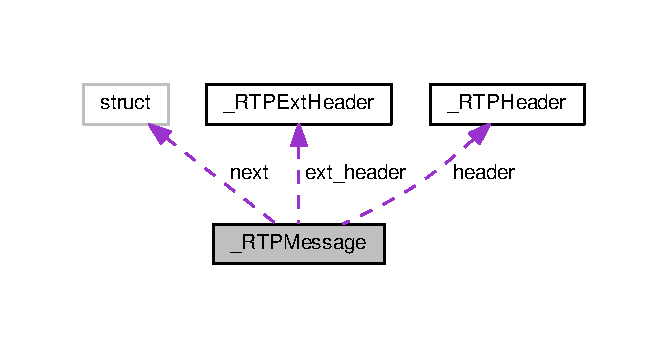
\includegraphics[width=321pt]{dc/d62/struct___r_t_p_message__coll__graph}
\end{center}
\end{figure}
\subsection*{Data Fields}
\begin{DoxyCompactItemize}
\item 
\hyperlink{rtp_8h_a75f2f434fb40aaadc6665cb0c9010e49}{R\+T\+P\+Header} $\ast$ \hyperlink{struct___r_t_p_message_afa0aee0d9eab5781c753943ec6a37584}{header}
\item 
\hyperlink{rtp_8h_ab384df54f92f379aa578740b96a3aaaa}{R\+T\+P\+Ext\+Header} $\ast$ \hyperlink{struct___r_t_p_message_aa0a69d899b1bee283ae1490f53bcd073}{ext\+\_\+header}
\item 
uint8\+\_\+t \hyperlink{struct___r_t_p_message_a89f8083b50c7cef74e96797bb74f8757}{data} \mbox{[}\hyperlink{rtp_8h_ac552c225344e6f60cbadb539fe35e6f5}{M\+A\+X\+\_\+\+R\+T\+P\+\_\+\+S\+I\+Z\+E}\mbox{]}
\item 
uint32\+\_\+t \hyperlink{struct___r_t_p_message_aebb70c2aab3407a9f05334c47131a43b}{length}
\item 
struct \hyperlink{struct___r_t_p_message}{\+\_\+\+R\+T\+P\+Message} $\ast$ \hyperlink{struct___r_t_p_message_af02d4bf6724c59e5df90bacdfc8a8499}{next}
\end{DoxyCompactItemize}


\subsection{Detailed Description}
Standard rtp message. 

Definition at line 64 of file rtp.\+h.



\subsection{Field Documentation}
\hypertarget{struct___r_t_p_message_a89f8083b50c7cef74e96797bb74f8757}{\index{\+\_\+\+R\+T\+P\+Message@{\+\_\+\+R\+T\+P\+Message}!data@{data}}
\index{data@{data}!\+\_\+\+R\+T\+P\+Message@{\+\_\+\+R\+T\+P\+Message}}
\subsubsection[{data}]{\setlength{\rightskip}{0pt plus 5cm}uint8\+\_\+t data\mbox{[}{\bf M\+A\+X\+\_\+\+R\+T\+P\+\_\+\+S\+I\+Z\+E}\mbox{]}}}\label{struct___r_t_p_message_a89f8083b50c7cef74e96797bb74f8757}


Definition at line 68 of file rtp.\+h.



Referenced by cs\+\_\+do(), msg\+\_\+parse(), queue\+\_\+message(), rtp\+\_\+new\+\_\+message(), and rtp\+\_\+send\+\_\+msg().

\hypertarget{struct___r_t_p_message_aa0a69d899b1bee283ae1490f53bcd073}{\index{\+\_\+\+R\+T\+P\+Message@{\+\_\+\+R\+T\+P\+Message}!ext\+\_\+header@{ext\+\_\+header}}
\index{ext\+\_\+header@{ext\+\_\+header}!\+\_\+\+R\+T\+P\+Message@{\+\_\+\+R\+T\+P\+Message}}
\subsubsection[{ext\+\_\+header}]{\setlength{\rightskip}{0pt plus 5cm}{\bf R\+T\+P\+Ext\+Header}$\ast$ ext\+\_\+header}}\label{struct___r_t_p_message_aa0a69d899b1bee283ae1490f53bcd073}


Definition at line 66 of file rtp.\+h.



Referenced by msg\+\_\+parse(), rtp\+\_\+free\+\_\+msg(), and rtp\+\_\+new\+\_\+message().

\hypertarget{struct___r_t_p_message_afa0aee0d9eab5781c753943ec6a37584}{\index{\+\_\+\+R\+T\+P\+Message@{\+\_\+\+R\+T\+P\+Message}!header@{header}}
\index{header@{header}!\+\_\+\+R\+T\+P\+Message@{\+\_\+\+R\+T\+P\+Message}}
\subsubsection[{header}]{\setlength{\rightskip}{0pt plus 5cm}{\bf R\+T\+P\+Header}$\ast$ header}}\label{struct___r_t_p_message_afa0aee0d9eab5781c753943ec6a37584}


Definition at line 65 of file rtp.\+h.



Referenced by check\+\_\+late\+\_\+message(), jbuf\+\_\+write(), msg\+\_\+parse(), queue\+\_\+message(), rtp\+\_\+free\+\_\+msg(), rtp\+\_\+handle\+\_\+packet(), and rtp\+\_\+new\+\_\+message().

\hypertarget{struct___r_t_p_message_aebb70c2aab3407a9f05334c47131a43b}{\index{\+\_\+\+R\+T\+P\+Message@{\+\_\+\+R\+T\+P\+Message}!length@{length}}
\index{length@{length}!\+\_\+\+R\+T\+P\+Message@{\+\_\+\+R\+T\+P\+Message}}
\subsubsection[{length}]{\setlength{\rightskip}{0pt plus 5cm}uint32\+\_\+t length}}\label{struct___r_t_p_message_aebb70c2aab3407a9f05334c47131a43b}


Definition at line 69 of file rtp.\+h.



Referenced by cs\+\_\+do(), msg\+\_\+parse(), queue\+\_\+message(), rtp\+\_\+new\+\_\+message(), and rtp\+\_\+send\+\_\+msg().

\hypertarget{struct___r_t_p_message_af02d4bf6724c59e5df90bacdfc8a8499}{\index{\+\_\+\+R\+T\+P\+Message@{\+\_\+\+R\+T\+P\+Message}!next@{next}}
\index{next@{next}!\+\_\+\+R\+T\+P\+Message@{\+\_\+\+R\+T\+P\+Message}}
\subsubsection[{next}]{\setlength{\rightskip}{0pt plus 5cm}struct {\bf \+\_\+\+R\+T\+P\+Message}$\ast$ next}}\label{struct___r_t_p_message_af02d4bf6724c59e5df90bacdfc8a8499}


Definition at line 71 of file rtp.\+h.



Referenced by msg\+\_\+parse(), and rtp\+\_\+new\+\_\+message().



The documentation for this struct was generated from the following file\+:\begin{DoxyCompactItemize}
\item 
toxav/\hyperlink{rtp_8h}{rtp.\+h}\end{DoxyCompactItemize}

\hypertarget{struct___r_t_p_session}{\section{\+\_\+\+R\+T\+P\+Session Struct Reference}
\label{struct___r_t_p_session}\index{\+\_\+\+R\+T\+P\+Session@{\+\_\+\+R\+T\+P\+Session}}
}


{\ttfamily \#include $<$rtp.\+h$>$}



Collaboration diagram for \+\_\+\+R\+T\+P\+Session\+:
\nopagebreak
\begin{figure}[H]
\begin{center}
\leavevmode
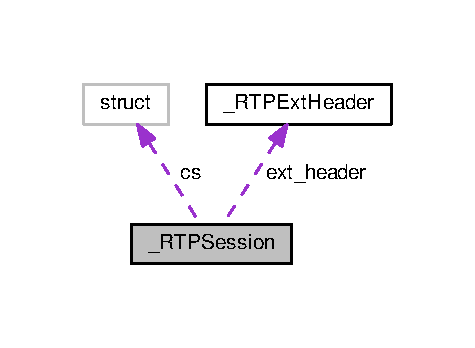
\includegraphics[width=228pt]{struct___r_t_p_session__coll__graph}
\end{center}
\end{figure}
\subsection*{Data Fields}
\begin{DoxyCompactItemize}
\item 
\hypertarget{struct___r_t_p_session_ab22abc2906422da61885ac6c8e6a1a59}{uint8\+\_\+t {\bfseries version}}\label{struct___r_t_p_session_ab22abc2906422da61885ac6c8e6a1a59}

\item 
\hypertarget{struct___r_t_p_session_a78a52d3de83ec4d91a7746456627089f}{uint8\+\_\+t {\bfseries padding}}\label{struct___r_t_p_session_a78a52d3de83ec4d91a7746456627089f}

\item 
\hypertarget{struct___r_t_p_session_a91c592cf70c61ba0788394767185be4c}{uint8\+\_\+t {\bfseries extension}}\label{struct___r_t_p_session_a91c592cf70c61ba0788394767185be4c}

\item 
\hypertarget{struct___r_t_p_session_a622e15900f3d90f1391cf9812d1a8078}{uint8\+\_\+t {\bfseries cc}}\label{struct___r_t_p_session_a622e15900f3d90f1391cf9812d1a8078}

\item 
\hypertarget{struct___r_t_p_session_ae00c35797c92d6f67470b088dc2c1876}{uint8\+\_\+t {\bfseries marker}}\label{struct___r_t_p_session_ae00c35797c92d6f67470b088dc2c1876}

\item 
\hypertarget{struct___r_t_p_session_a9cdef377149cce5efd90b1e60596573a}{uint8\+\_\+t {\bfseries payload\+\_\+type}}\label{struct___r_t_p_session_a9cdef377149cce5efd90b1e60596573a}

\item 
\hypertarget{struct___r_t_p_session_afe208c7dec97b8f61e08094e61bf096e}{uint16\+\_\+t {\bfseries sequnum}}\label{struct___r_t_p_session_afe208c7dec97b8f61e08094e61bf096e}

\item 
\hypertarget{struct___r_t_p_session_a1bef56c38f8d3bc3ab5d381e11c29d0d}{uint16\+\_\+t {\bfseries rsequnum}}\label{struct___r_t_p_session_a1bef56c38f8d3bc3ab5d381e11c29d0d}

\item 
\hypertarget{struct___r_t_p_session_ab20b0c7772544cf5d318507f34231fbe}{uint32\+\_\+t {\bfseries timestamp}}\label{struct___r_t_p_session_ab20b0c7772544cf5d318507f34231fbe}

\item 
\hypertarget{struct___r_t_p_session_a7728cdfcf33cc14c0d7ba2dcdcbcdf2e}{uint32\+\_\+t {\bfseries ssrc}}\label{struct___r_t_p_session_a7728cdfcf33cc14c0d7ba2dcdcbcdf2e}

\item 
\hypertarget{struct___r_t_p_session_a8bbd14e68a057e6de8ba3fa4c6afd4fa}{uint32\+\_\+t $\ast$ {\bfseries csrc}}\label{struct___r_t_p_session_a8bbd14e68a057e6de8ba3fa4c6afd4fa}

\item 
\hypertarget{struct___r_t_p_session_aa0a69d899b1bee283ae1490f53bcd073}{\hyperlink{struct___r_t_p_ext_header}{R\+T\+P\+Ext\+Header} $\ast$ {\bfseries ext\+\_\+header}}\label{struct___r_t_p_session_aa0a69d899b1bee283ae1490f53bcd073}

\item 
\hypertarget{struct___r_t_p_session_acf4a7a7457f3d922d7118075fc1a300b}{uint8\+\_\+t {\bfseries prefix}}\label{struct___r_t_p_session_acf4a7a7457f3d922d7118075fc1a300b}

\item 
\hypertarget{struct___r_t_p_session_ae5163ff230abd4115d86194ad89467b5}{int {\bfseries dest}}\label{struct___r_t_p_session_ae5163ff230abd4115d86194ad89467b5}

\item 
\hypertarget{struct___r_t_p_session_a6fa710f1d7103d0f7b2b872e33aac143}{struct \hyperlink{struct___c_s_session}{\+\_\+\+C\+S\+Session} $\ast$ {\bfseries cs}}\label{struct___r_t_p_session_a6fa710f1d7103d0f7b2b872e33aac143}

\end{DoxyCompactItemize}


\subsection{Detailed Description}
R\+T\+P control session. 

Definition at line 77 of file rtp.\+h.



The documentation for this struct was generated from the following file\+:\begin{DoxyCompactItemize}
\item 
toxav/rtp.\+h\end{DoxyCompactItemize}

\hypertarget{struct___status}{\section{\+\_\+\+Status Struct Reference}
\label{struct___status}\index{\+\_\+\+Status@{\+\_\+\+Status}}
}


Collaboration diagram for \+\_\+\+Status\+:\nopagebreak
\begin{figure}[H]
\begin{center}
\leavevmode
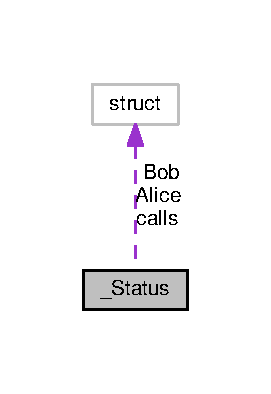
\includegraphics[width=130pt]{struct___status__coll__graph}
\end{center}
\end{figure}
\subsection*{Data Fields}
\begin{DoxyCompactItemize}
\item 
\hypertarget{struct___status_a0fd20957e107227630b542b146c276d4}{\hyperlink{struct___party}{Party} {\bfseries Alice}}\label{struct___status_a0fd20957e107227630b542b146c276d4}

\item 
\hypertarget{struct___status_a78cf423939bd332fd6e5ddae67134e01}{\hyperlink{struct___party}{Party} {\bfseries Bob}}\label{struct___status_a78cf423939bd332fd6e5ddae67134e01}

\item 
\hypertarget{struct___status_a2f6221bbb611e0d485e26cd2722bd7ee}{\hyperlink{struct___a_call}{A\+Call} {\bfseries calls} \mbox{[}3\mbox{]}}\label{struct___status_a2f6221bbb611e0d485e26cd2722bd7ee}

\end{DoxyCompactItemize}


\subsection{Detailed Description}


Definition at line 50 of file toxav\+\_\+basic\+\_\+test.\+c.



The documentation for this struct was generated from the following files\+:\begin{DoxyCompactItemize}
\item 
auto\+\_\+tests/toxav\+\_\+basic\+\_\+test.\+c\item 
auto\+\_\+tests/toxav\+\_\+many\+\_\+test.\+c\end{DoxyCompactItemize}

\hypertarget{struct___timer}{\section{\+\_\+\+Timer Struct Reference}
\label{struct___timer}\index{\+\_\+\+Timer@{\+\_\+\+Timer}}
}


Collaboration diagram for \+\_\+\+Timer\+:\nopagebreak
\begin{figure}[H]
\begin{center}
\leavevmode
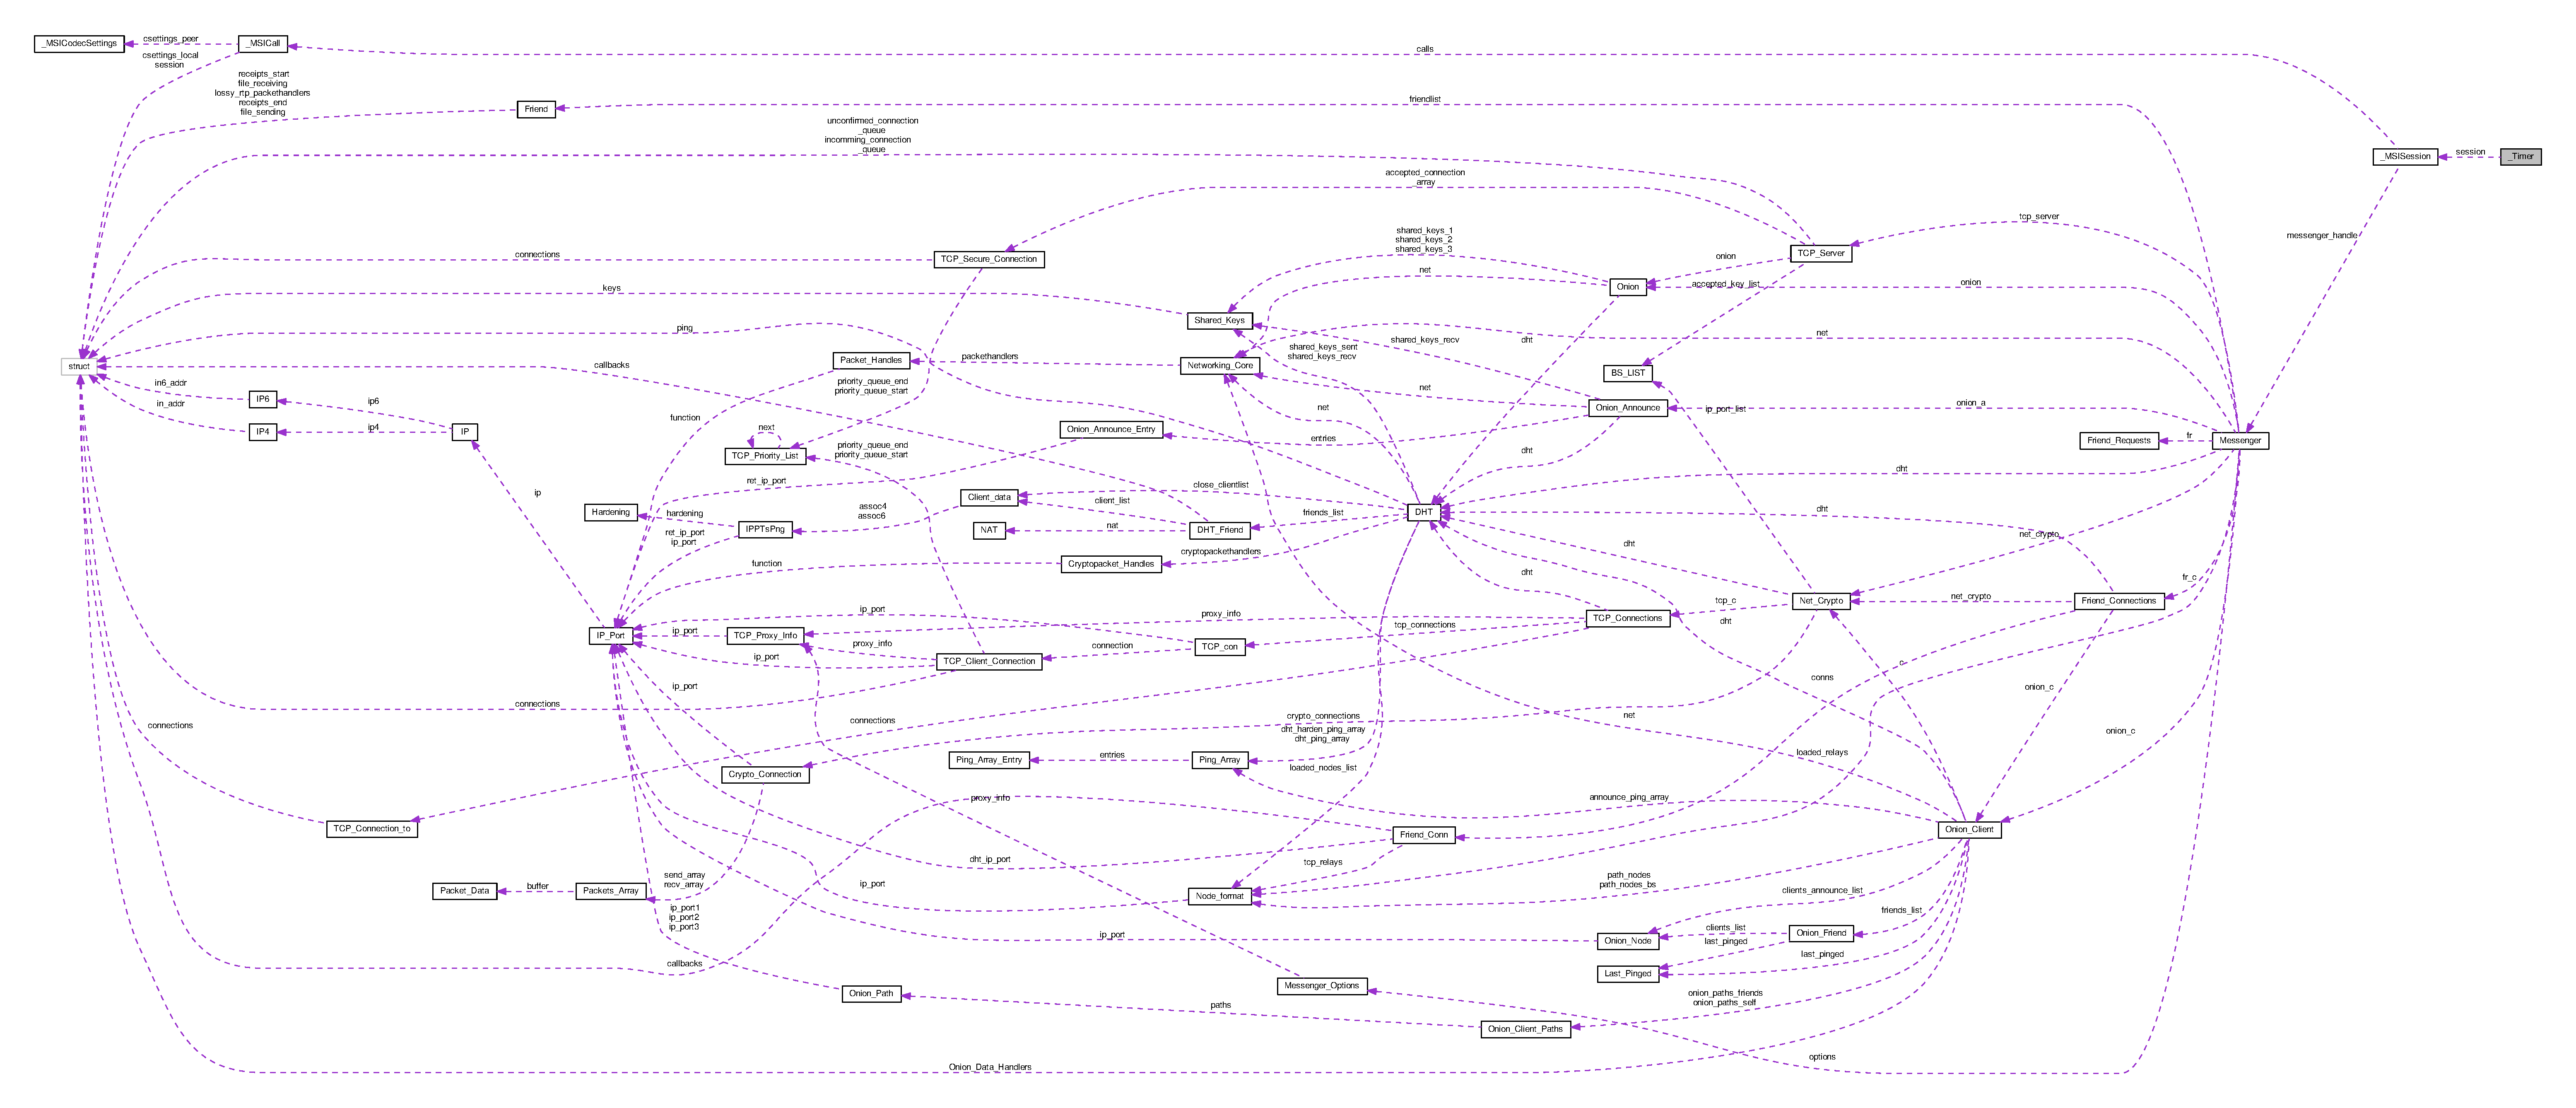
\includegraphics[width=350pt]{struct___timer__coll__graph}
\end{center}
\end{figure}
\subsection*{Data Fields}
\begin{DoxyCompactItemize}
\item 
\hypertarget{struct___timer_a7b75ecf42c49a289b6dd4fefdbf86605}{void($\ast$ {\bfseries func} )(struct \hyperlink{struct___timer}{\+\_\+\+Timer} $\ast$)}\label{struct___timer_a7b75ecf42c49a289b6dd4fefdbf86605}

\item 
\hypertarget{struct___timer_a053cdea1d85795444fe1aaa6b277a0ec}{uint64\+\_\+t {\bfseries timeout}}\label{struct___timer_a053cdea1d85795444fe1aaa6b277a0ec}

\item 
\hypertarget{struct___timer_affcb6f96b80aecebae0f1b157c6242b5}{\hyperlink{struct___m_s_i_session}{M\+S\+I\+Session} $\ast$ {\bfseries session}}\label{struct___timer_affcb6f96b80aecebae0f1b157c6242b5}

\item 
\hypertarget{struct___timer_a1137c8c8a662d51868eda69bd73915d0}{int {\bfseries call\+\_\+idx}}\label{struct___timer_a1137c8c8a662d51868eda69bd73915d0}

\item 
\hypertarget{struct___timer_a7441ef0865bcb3db9b8064dd7375c1ea}{int {\bfseries id}}\label{struct___timer_a7441ef0865bcb3db9b8064dd7375c1ea}

\end{DoxyCompactItemize}


\subsection{Detailed Description}


Definition at line 427 of file msi.\+c.



The documentation for this struct was generated from the following file\+:\begin{DoxyCompactItemize}
\item 
toxav/msi.\+c\end{DoxyCompactItemize}

\hypertarget{struct___timer_handler}{\section{\+\_\+\+Timer\+Handler Struct Reference}
\label{struct___timer_handler}\index{\+\_\+\+Timer\+Handler@{\+\_\+\+Timer\+Handler}}
}


Collaboration diagram for \+\_\+\+Timer\+Handler\+:\nopagebreak
\begin{figure}[H]
\begin{center}
\leavevmode
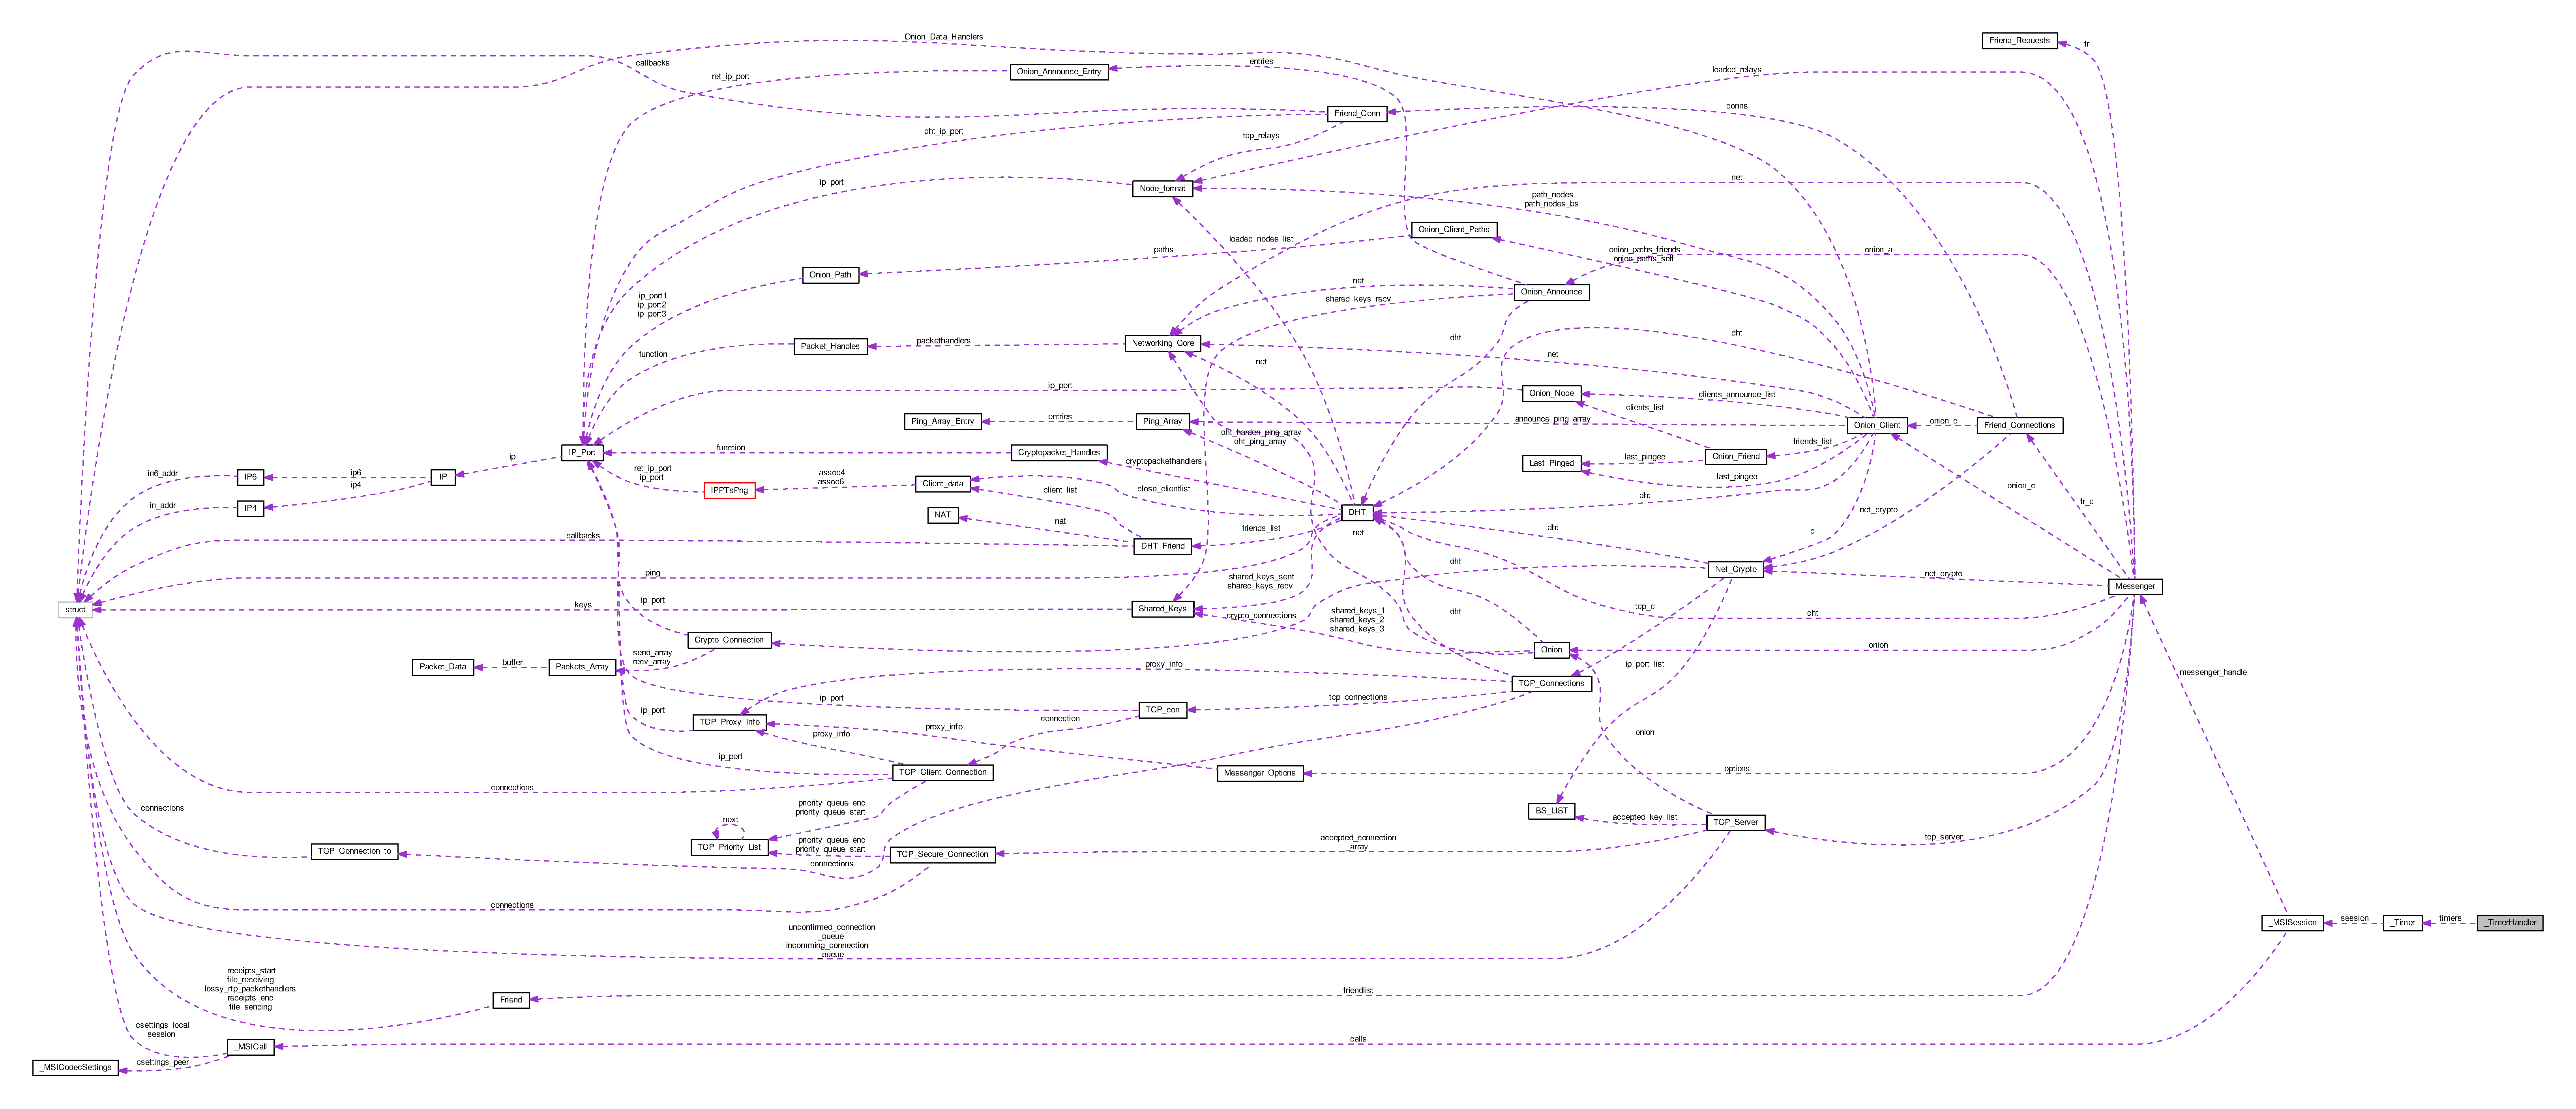
\includegraphics[width=350pt]{struct___timer_handler__coll__graph}
\end{center}
\end{figure}
\subsection*{Data Fields}
\begin{DoxyCompactItemize}
\item 
\hypertarget{struct___timer_handler_af6a69553fb8462326147c121a4c3e98c}{\hyperlink{struct___timer}{Timer} $\ast$$\ast$ {\bfseries timers}}\label{struct___timer_handler_af6a69553fb8462326147c121a4c3e98c}

\item 
\hypertarget{struct___timer_handler_a75d656828e87eb82559cb02fa2219d98}{uint32\+\_\+t {\bfseries max\+\_\+capacity}}\label{struct___timer_handler_a75d656828e87eb82559cb02fa2219d98}

\item 
\hypertarget{struct___timer_handler_ab2c6b258f02add8fdf4cfc7c371dd772}{uint32\+\_\+t {\bfseries size}}\label{struct___timer_handler_ab2c6b258f02add8fdf4cfc7c371dd772}

\end{DoxyCompactItemize}


\subsection{Detailed Description}


Definition at line 436 of file msi.\+c.



The documentation for this struct was generated from the following file\+:\begin{DoxyCompactItemize}
\item 
toxav/msi.\+c\end{DoxyCompactItemize}

\hypertarget{struct___tox_av}{\section{\+\_\+\+Tox\+Av Struct Reference}
\label{struct___tox_av}\index{\+\_\+\+Tox\+Av@{\+\_\+\+Tox\+Av}}
}


Collaboration diagram for \+\_\+\+Tox\+Av\+:
\nopagebreak
\begin{figure}[H]
\begin{center}
\leavevmode
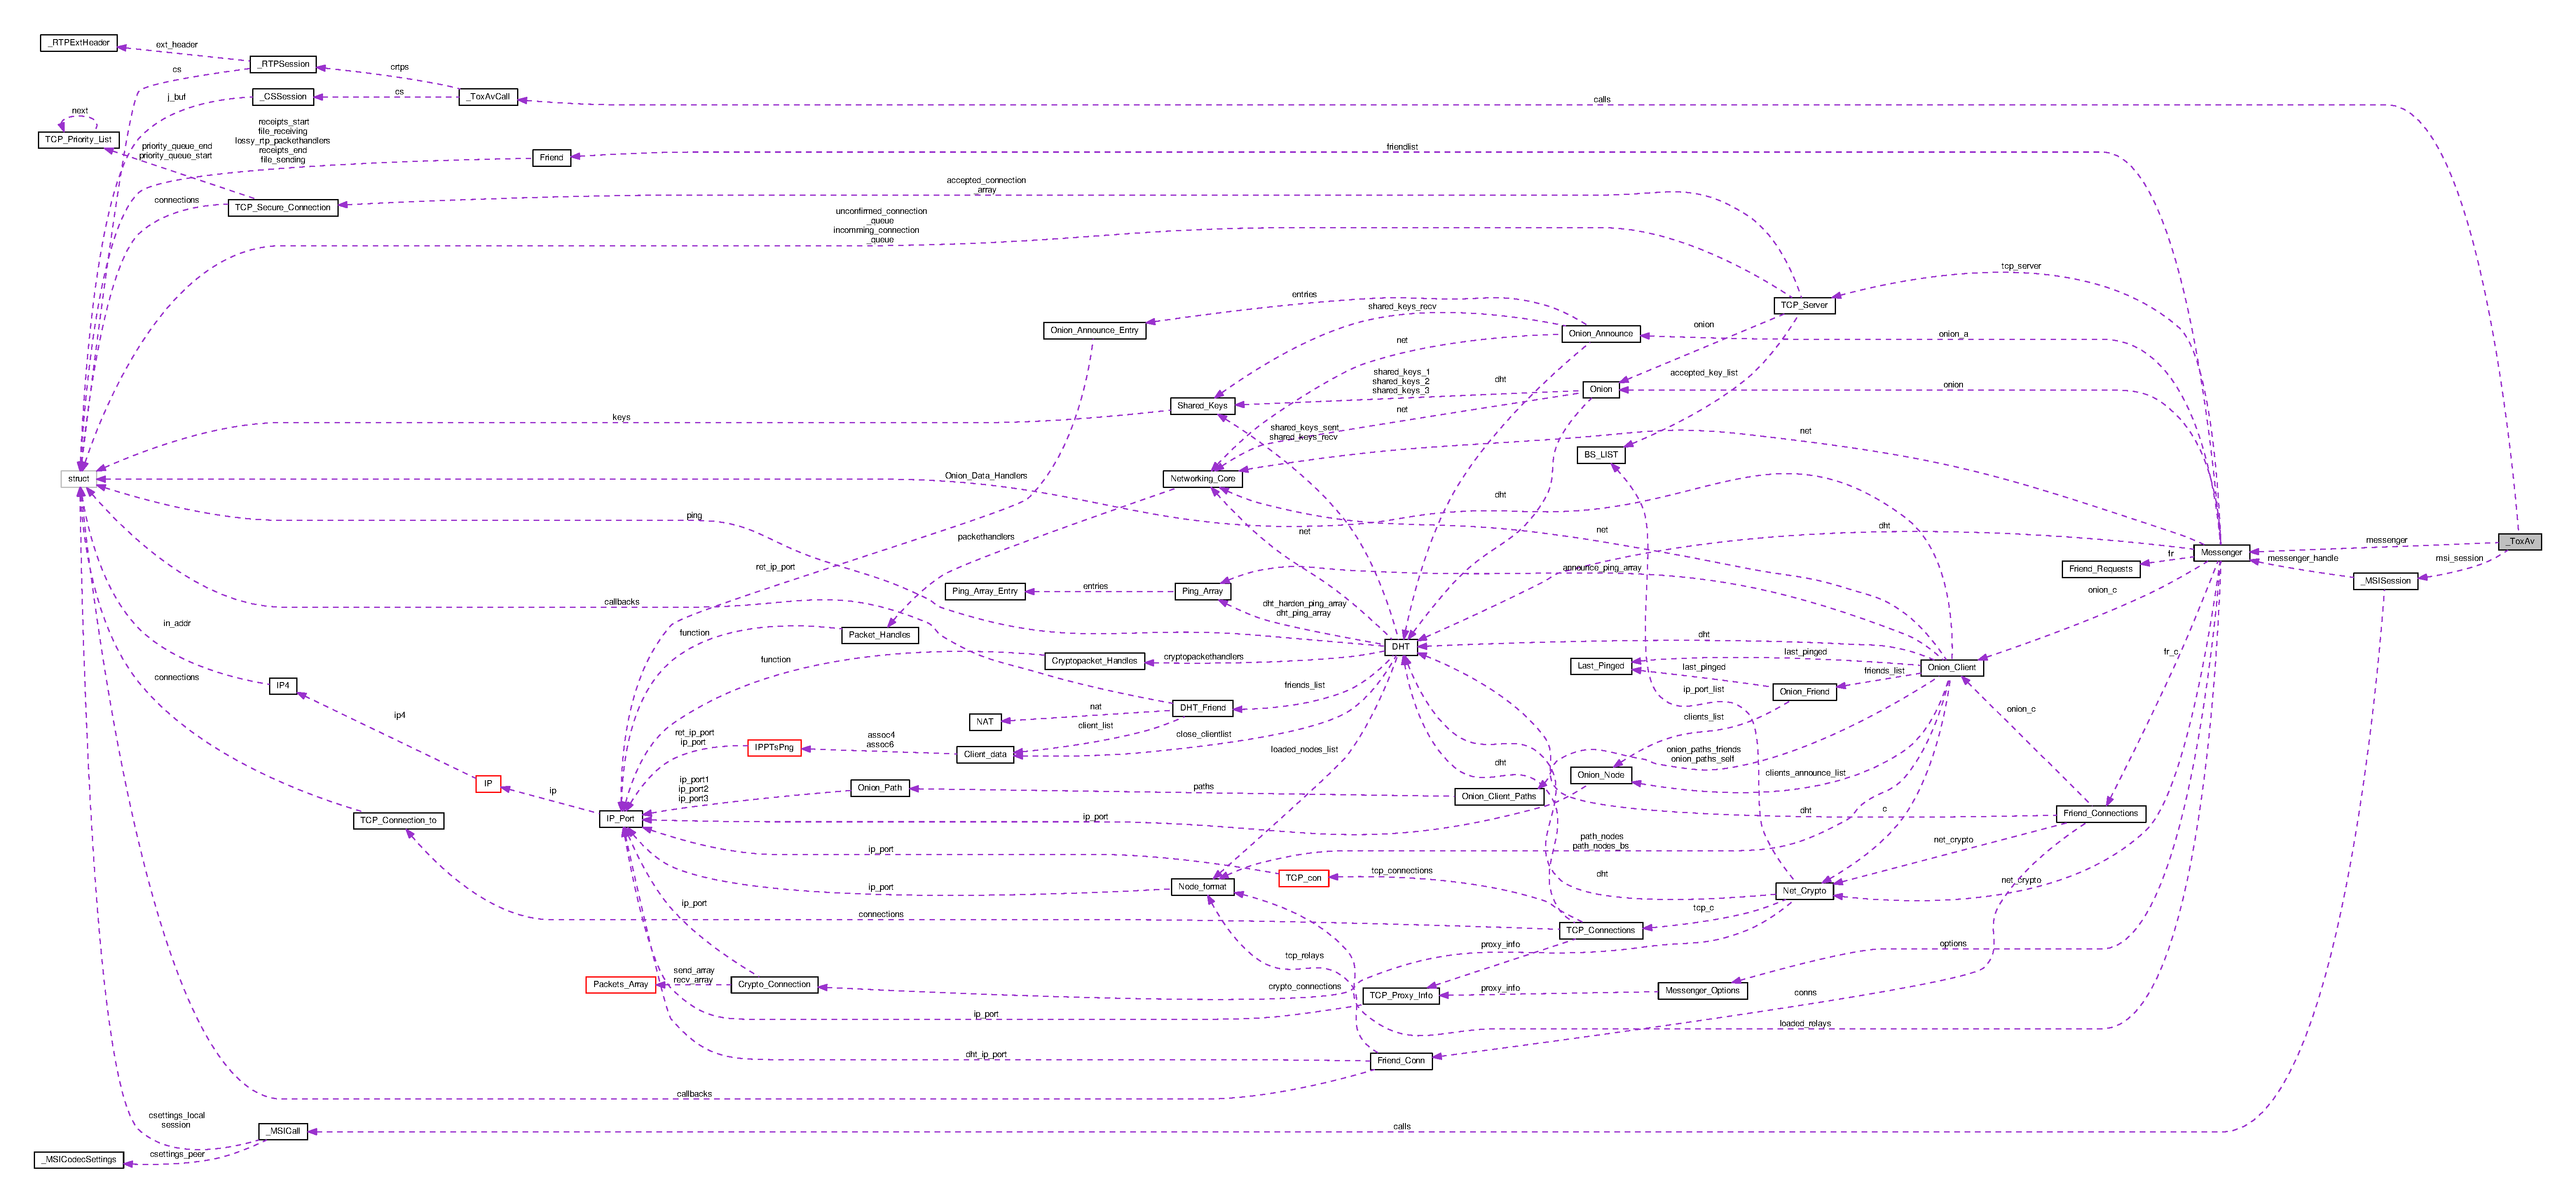
\includegraphics[width=350pt]{d9/d45/struct___tox_av__coll__graph}
\end{center}
\end{figure}
\subsection*{Data Fields}
\begin{DoxyCompactItemize}
\item 
\hyperlink{struct_messenger}{Messenger} $\ast$ \hyperlink{struct___tox_av_a48342badc24a04d2310ca16ff4a3711b}{messenger}
\item 
\hyperlink{msi_8h_adc69aa9b8f2f21b2b54e542cc9bb4329}{M\+S\+I\+Session} $\ast$ \hyperlink{struct___tox_av_a85e3d7dd2ab722ee5ba0cd4b72bc7d60}{msi\+\_\+session}
\item 
\hyperlink{toxav_8c_aec40f142d19ca255ccdf4097b03ef51e}{Tox\+Av\+Call} $\ast$ \hyperlink{struct___tox_av_abe854f89ac28ebd5112d1639d531b128}{calls}
\item 
uint32\+\_\+t \hyperlink{struct___tox_av_a7d6cf32eb812384ebd4074c588c17499}{max\+\_\+calls}
\end{DoxyCompactItemize}


\subsection{Detailed Description}


Definition at line 74 of file toxav.\+c.



\subsection{Field Documentation}
\hypertarget{struct___tox_av_abe854f89ac28ebd5112d1639d531b128}{\index{\+\_\+\+Tox\+Av@{\+\_\+\+Tox\+Av}!calls@{calls}}
\index{calls@{calls}!\+\_\+\+Tox\+Av@{\+\_\+\+Tox\+Av}}
\subsubsection[{calls}]{\setlength{\rightskip}{0pt plus 5cm}{\bf Tox\+Av\+Call}$\ast$ calls}}\label{struct___tox_av_abe854f89ac28ebd5112d1639d531b128}
Main msi session 

Definition at line 77 of file toxav.\+c.



Referenced by toxav\+\_\+capability\+\_\+supported(), toxav\+\_\+do(), toxav\+\_\+do\+\_\+interval(), toxav\+\_\+get\+\_\+active\+\_\+count(), toxav\+\_\+kill(), toxav\+\_\+kill\+\_\+transmission(), toxav\+\_\+new(), toxav\+\_\+prepare\+\_\+audio\+\_\+frame(), toxav\+\_\+prepare\+\_\+transmission(), toxav\+\_\+prepare\+\_\+video\+\_\+frame(), toxav\+\_\+send\+\_\+audio(), and toxav\+\_\+send\+\_\+video().

\hypertarget{struct___tox_av_a7d6cf32eb812384ebd4074c588c17499}{\index{\+\_\+\+Tox\+Av@{\+\_\+\+Tox\+Av}!max\+\_\+calls@{max\+\_\+calls}}
\index{max\+\_\+calls@{max\+\_\+calls}!\+\_\+\+Tox\+Av@{\+\_\+\+Tox\+Av}}
\subsubsection[{max\+\_\+calls}]{\setlength{\rightskip}{0pt plus 5cm}uint32\+\_\+t max\+\_\+calls}}\label{struct___tox_av_a7d6cf32eb812384ebd4074c588c17499}
Per-\/call params 

Definition at line 78 of file toxav.\+c.



Referenced by toxav\+\_\+do(), toxav\+\_\+do\+\_\+interval(), toxav\+\_\+get\+\_\+active\+\_\+count(), toxav\+\_\+kill(), and toxav\+\_\+new().

\hypertarget{struct___tox_av_a48342badc24a04d2310ca16ff4a3711b}{\index{\+\_\+\+Tox\+Av@{\+\_\+\+Tox\+Av}!messenger@{messenger}}
\index{messenger@{messenger}!\+\_\+\+Tox\+Av@{\+\_\+\+Tox\+Av}}
\subsubsection[{messenger}]{\setlength{\rightskip}{0pt plus 5cm}{\bf Messenger}$\ast$ messenger}}\label{struct___tox_av_a48342badc24a04d2310ca16ff4a3711b}


Definition at line 75 of file toxav.\+c.



Referenced by toxav\+\_\+get\+\_\+tox(), toxav\+\_\+kill\+\_\+transmission(), toxav\+\_\+new(), toxav\+\_\+prepare\+\_\+transmission(), and toxav\+\_\+send\+\_\+rtp\+\_\+payload().

\hypertarget{struct___tox_av_a85e3d7dd2ab722ee5ba0cd4b72bc7d60}{\index{\+\_\+\+Tox\+Av@{\+\_\+\+Tox\+Av}!msi\+\_\+session@{msi\+\_\+session}}
\index{msi\+\_\+session@{msi\+\_\+session}!\+\_\+\+Tox\+Av@{\+\_\+\+Tox\+Av}}
\subsubsection[{msi\+\_\+session}]{\setlength{\rightskip}{0pt plus 5cm}{\bf M\+S\+I\+Session}$\ast$ msi\+\_\+session}}\label{struct___tox_av_a85e3d7dd2ab722ee5ba0cd4b72bc7d60}


Definition at line 76 of file toxav.\+c.



Referenced by toxav\+\_\+answer(), toxav\+\_\+call(), toxav\+\_\+cancel(), toxav\+\_\+change\+\_\+settings(), toxav\+\_\+do(), toxav\+\_\+get\+\_\+call\+\_\+state(), toxav\+\_\+get\+\_\+peer\+\_\+csettings(), toxav\+\_\+get\+\_\+peer\+\_\+id(), toxav\+\_\+hangup(), toxav\+\_\+kill(), toxav\+\_\+kill\+\_\+transmission(), toxav\+\_\+new(), toxav\+\_\+prepare\+\_\+audio\+\_\+frame(), toxav\+\_\+prepare\+\_\+transmission(), toxav\+\_\+prepare\+\_\+video\+\_\+frame(), toxav\+\_\+register\+\_\+callstate\+\_\+callback(), toxav\+\_\+reject(), toxav\+\_\+send\+\_\+audio(), toxav\+\_\+send\+\_\+video(), and toxav\+\_\+stop\+\_\+call().



The documentation for this struct was generated from the following file\+:\begin{DoxyCompactItemize}
\item 
toxav/\hyperlink{toxav_8c}{toxav.\+c}\end{DoxyCompactItemize}

\hypertarget{struct___tox_av_call}{\section{\+\_\+\+Tox\+Av\+Call Struct Reference}
\label{struct___tox_av_call}\index{\+\_\+\+Tox\+Av\+Call@{\+\_\+\+Tox\+Av\+Call}}
}


Collaboration diagram for \+\_\+\+Tox\+Av\+Call\+:
\nopagebreak
\begin{figure}[H]
\begin{center}
\leavevmode
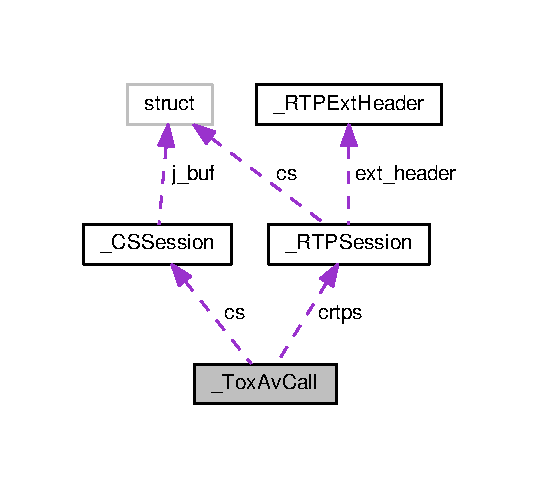
\includegraphics[width=260pt]{struct___tox_av_call__coll__graph}
\end{center}
\end{figure}
\subsection*{Data Fields}
\begin{DoxyCompactItemize}
\item 
\hypertarget{struct___tox_av_call_ab4293016252c4d4e63549b0773fa0f33}{pthread\+\_\+mutex\+\_\+t {\bfseries mutex} \mbox{[}1\mbox{]}}\label{struct___tox_av_call_ab4293016252c4d4e63549b0773fa0f33}

\item 
\hypertarget{struct___tox_av_call_ac4c859b6e4ff8e175151fbd0a763e414}{pthread\+\_\+mutex\+\_\+t {\bfseries mutex\+\_\+encoding\+\_\+audio} \mbox{[}1\mbox{]}}\label{struct___tox_av_call_ac4c859b6e4ff8e175151fbd0a763e414}

\item 
\hypertarget{struct___tox_av_call_a89e9fe0c3fef08c502e53ad423dccc34}{pthread\+\_\+mutex\+\_\+t {\bfseries mutex\+\_\+encoding\+\_\+video} \mbox{[}1\mbox{]}}\label{struct___tox_av_call_a89e9fe0c3fef08c502e53ad423dccc34}

\item 
\hypertarget{struct___tox_av_call_acc4203df7776b6dfe0e5c3922a35e5b0}{pthread\+\_\+mutex\+\_\+t {\bfseries mutex\+\_\+do} \mbox{[}1\mbox{]}}\label{struct___tox_av_call_acc4203df7776b6dfe0e5c3922a35e5b0}

\item 
\hypertarget{struct___tox_av_call_a2e84bee4a1898deac1f63f47235378eb}{\hyperlink{struct___r_t_p_session}{R\+T\+P\+Session} $\ast$ {\bfseries crtps} \mbox{[}2\mbox{]}}\label{struct___tox_av_call_a2e84bee4a1898deac1f63f47235378eb}

\item 
\hyperlink{struct___c_s_session}{C\+S\+Session} $\ast$ \hyperlink{struct___tox_av_call_ae88a02b5082b346e4c90541186364e99}{cs}
\item 
\hypertarget{struct___tox_av_call_a215df53a125f9b848dc883d9a1164430}{\+\_\+\+Bool {\bfseries active}}\label{struct___tox_av_call_a215df53a125f9b848dc883d9a1164430}

\end{DoxyCompactItemize}


\subsection{Detailed Description}


Definition at line 64 of file toxav.\+c.



\subsection{Field Documentation}
\hypertarget{struct___tox_av_call_ae88a02b5082b346e4c90541186364e99}{\index{\+\_\+\+Tox\+Av\+Call@{\+\_\+\+Tox\+Av\+Call}!cs@{cs}}
\index{cs@{cs}!\+\_\+\+Tox\+Av\+Call@{\+\_\+\+Tox\+Av\+Call}}
\subsubsection[{cs}]{\setlength{\rightskip}{0pt plus 5cm}{\bf C\+S\+Session}$\ast$ cs}}\label{struct___tox_av_call_ae88a02b5082b346e4c90541186364e99}
Audio is first and video is second 

Definition at line 70 of file toxav.\+c.



The documentation for this struct was generated from the following file\+:\begin{DoxyCompactItemize}
\item 
toxav/toxav.\+c\end{DoxyCompactItemize}

\hypertarget{struct___tox_av_c_settings}{\section{\+\_\+\+Tox\+Av\+C\+Settings Struct Reference}
\label{struct___tox_av_c_settings}\index{\+\_\+\+Tox\+Av\+C\+Settings@{\+\_\+\+Tox\+Av\+C\+Settings}}
}


{\ttfamily \#include $<$toxav.\+h$>$}

\subsection*{Data Fields}
\begin{DoxyCompactItemize}
\item 
\hypertarget{struct___tox_av_c_settings_af8142c751283bdc9d14609ab3009b920}{Tox\+Av\+Call\+Type {\bfseries call\+\_\+type}}\label{struct___tox_av_c_settings_af8142c751283bdc9d14609ab3009b920}

\item 
\hypertarget{struct___tox_av_c_settings_af0eac99d4181795e8a595d244e745192}{uint32\+\_\+t {\bfseries video\+\_\+bitrate}}\label{struct___tox_av_c_settings_af0eac99d4181795e8a595d244e745192}

\item 
\hypertarget{struct___tox_av_c_settings_ab81ecded1f7c46e120c8f2afa7b2c5cc}{uint16\+\_\+t {\bfseries max\+\_\+video\+\_\+width}}\label{struct___tox_av_c_settings_ab81ecded1f7c46e120c8f2afa7b2c5cc}

\item 
\hypertarget{struct___tox_av_c_settings_a4fef4b2fa1a8ae8446314ad0af4ce698}{uint16\+\_\+t {\bfseries max\+\_\+video\+\_\+height}}\label{struct___tox_av_c_settings_a4fef4b2fa1a8ae8446314ad0af4ce698}

\item 
\hypertarget{struct___tox_av_c_settings_a5d9a8b59b2eb1eef8dbdcb032bf1dd01}{uint32\+\_\+t {\bfseries audio\+\_\+bitrate}}\label{struct___tox_av_c_settings_a5d9a8b59b2eb1eef8dbdcb032bf1dd01}

\item 
\hypertarget{struct___tox_av_c_settings_a61b592233f5a65705eb2600d38e365cd}{uint16\+\_\+t {\bfseries audio\+\_\+frame\+\_\+duration}}\label{struct___tox_av_c_settings_a61b592233f5a65705eb2600d38e365cd}

\item 
\hypertarget{struct___tox_av_c_settings_a66da4482e934a2700e07a39fa0838559}{uint32\+\_\+t {\bfseries audio\+\_\+sample\+\_\+rate}}\label{struct___tox_av_c_settings_a66da4482e934a2700e07a39fa0838559}

\item 
\hypertarget{struct___tox_av_c_settings_a1b04e9669a2929f425e867440b6d826d}{uint32\+\_\+t {\bfseries audio\+\_\+channels}}\label{struct___tox_av_c_settings_a1b04e9669a2929f425e867440b6d826d}

\end{DoxyCompactItemize}


\subsection{Detailed Description}
Encoding settings. 

Definition at line 121 of file toxav.\+h.



The documentation for this struct was generated from the following file\+:\begin{DoxyCompactItemize}
\item 
toxav/toxav.\+h\end{DoxyCompactItemize}

\hypertarget{struct_assoc}{\section{Assoc Struct Reference}
\label{struct_assoc}\index{Assoc@{Assoc}}
}


Collaboration diagram for Assoc\+:
\nopagebreak
\begin{figure}[H]
\begin{center}
\leavevmode
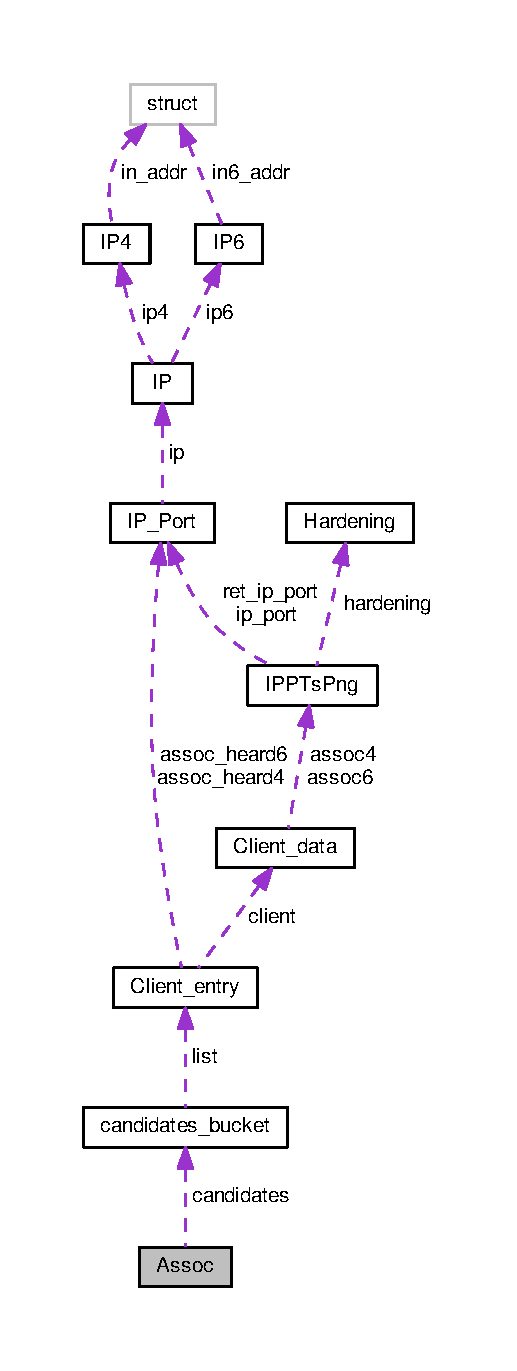
\includegraphics[height=550pt]{struct_assoc__coll__graph}
\end{center}
\end{figure}
\subsection*{Data Fields}
\begin{DoxyCompactItemize}
\item 
\hypertarget{struct_assoc_a6531d0c8e69576ae8c58a02914abaefe}{hash\+\_\+t {\bfseries self\+\_\+hash}}\label{struct_assoc_a6531d0c8e69576ae8c58a02914abaefe}

\item 
\hypertarget{struct_assoc_a509ad2eff925992e4ad8739d6fe2d7bb}{uint8\+\_\+t {\bfseries self\+\_\+client\+\_\+id} \mbox{[}C\+L\+I\+E\+N\+T\+\_\+\+I\+D\+\_\+\+S\+I\+Z\+E\mbox{]}}\label{struct_assoc_a509ad2eff925992e4ad8739d6fe2d7bb}

\item 
\hypertarget{struct_assoc_ab4153986e9b7dd71547967436299a424}{size\+\_\+t {\bfseries candidates\+\_\+bucket\+\_\+bits}}\label{struct_assoc_ab4153986e9b7dd71547967436299a424}

\item 
\hypertarget{struct_assoc_a22dd0674eae131fab27462b931d4397c}{size\+\_\+t {\bfseries candidates\+\_\+bucket\+\_\+count}}\label{struct_assoc_a22dd0674eae131fab27462b931d4397c}

\item 
\hypertarget{struct_assoc_a9349f5b3095733f74b3704aa9766a05a}{size\+\_\+t {\bfseries candidates\+\_\+bucket\+\_\+size}}\label{struct_assoc_a9349f5b3095733f74b3704aa9766a05a}

\item 
\hypertarget{struct_assoc_a9d492ea4282a0aca2bcb32d987f58175}{\hyperlink{structcandidates__bucket}{candidates\+\_\+bucket} $\ast$ {\bfseries candidates}}\label{struct_assoc_a9d492ea4282a0aca2bcb32d987f58175}

\item 
\hypertarget{struct_assoc_aec732782691c39a31d8c579a79a8fed2}{uint64\+\_\+t {\bfseries getnodes}}\label{struct_assoc_aec732782691c39a31d8c579a79a8fed2}

\end{DoxyCompactItemize}


\subsection{Detailed Description}


Definition at line 88 of file assoc.\+c.



The documentation for this struct was generated from the following file\+:\begin{DoxyCompactItemize}
\item 
toxcore/assoc.\+c\end{DoxyCompactItemize}

\hypertarget{struct_assoc__close__entries}{\section{Assoc\+\_\+close\+\_\+entries Struct Reference}
\label{struct_assoc__close__entries}\index{Assoc\+\_\+close\+\_\+entries@{Assoc\+\_\+close\+\_\+entries}}
}


Collaboration diagram for Assoc\+\_\+close\+\_\+entries\+:\nopagebreak
\begin{figure}[H]
\begin{center}
\leavevmode
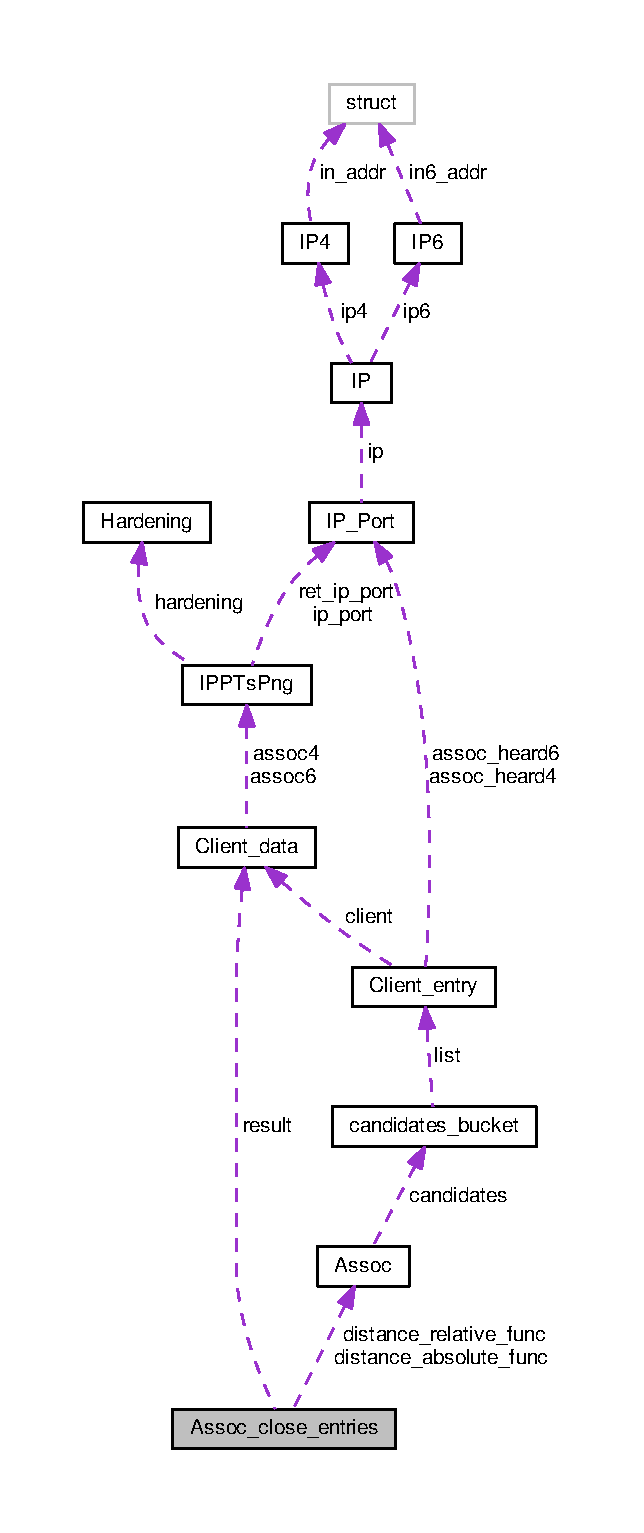
\includegraphics[height=550pt]{struct_assoc__close__entries__coll__graph}
\end{center}
\end{figure}
\subsection*{Data Fields}
\begin{DoxyCompactItemize}
\item 
\hypertarget{struct_assoc__close__entries_a89491b1d291e113f86c1d33a3c1ec66b}{void $\ast$ {\bfseries custom\+\_\+data}}\label{struct_assoc__close__entries_a89491b1d291e113f86c1d33a3c1ec66b}

\item 
\hypertarget{struct_assoc__close__entries_a037b65164e78b02017bd4751843037b4}{uint8\+\_\+t $\ast$ {\bfseries wanted\+\_\+id}}\label{struct_assoc__close__entries_a037b65164e78b02017bd4751843037b4}

\item 
\hypertarget{struct_assoc__close__entries_aa2585d779da0ab21273a8d92de9a0ebe}{uint8\+\_\+t {\bfseries flags}}\label{struct_assoc__close__entries_aa2585d779da0ab21273a8d92de9a0ebe}

\item 
\hypertarget{struct_assoc__close__entries_ada046356cf0fe3d4a2c18ac174d5eb0e}{Assoc\+\_\+distance\+\_\+relative\+\_\+callback {\bfseries distance\+\_\+relative\+\_\+func}}\label{struct_assoc__close__entries_ada046356cf0fe3d4a2c18ac174d5eb0e}

\item 
\hypertarget{struct_assoc__close__entries_aedd1522117fb10fb74c7054f25f2d282}{Assoc\+\_\+distance\+\_\+absolute\+\_\+callback {\bfseries distance\+\_\+absolute\+\_\+func}}\label{struct_assoc__close__entries_aedd1522117fb10fb74c7054f25f2d282}

\item 
\hypertarget{struct_assoc__close__entries_a086e0ce002c9491e4b99956740bb53d4}{uint8\+\_\+t {\bfseries count\+\_\+good}}\label{struct_assoc__close__entries_a086e0ce002c9491e4b99956740bb53d4}

\item 
\hypertarget{struct_assoc__close__entries_a20302e2c99a60d3f612dba57e3f6333b}{uint8\+\_\+t {\bfseries count}}\label{struct_assoc__close__entries_a20302e2c99a60d3f612dba57e3f6333b}

\item 
\hypertarget{struct_assoc__close__entries_a40d6704f891338dadfa89f46b696be4c}{\hyperlink{struct_client__data}{Client\+\_\+data} $\ast$$\ast$ {\bfseries result}}\label{struct_assoc__close__entries_a40d6704f891338dadfa89f46b696be4c}

\end{DoxyCompactItemize}


\subsection{Detailed Description}


Definition at line 49 of file assoc.\+h.



The documentation for this struct was generated from the following file\+:\begin{DoxyCompactItemize}
\item 
toxcore/assoc.\+h\end{DoxyCompactItemize}

\hypertarget{struct_b_s___l_i_s_t}{\section{B\+S\+\_\+\+L\+I\+S\+T Struct Reference}
\label{struct_b_s___l_i_s_t}\index{B\+S\+\_\+\+L\+I\+S\+T@{B\+S\+\_\+\+L\+I\+S\+T}}
}
\subsection*{Data Fields}
\begin{DoxyCompactItemize}
\item 
\hypertarget{struct_b_s___l_i_s_t_a3d8a9527a2ee4a7ebf59175650142e75}{uint32\+\_\+t {\bfseries n}}\label{struct_b_s___l_i_s_t_a3d8a9527a2ee4a7ebf59175650142e75}

\item 
\hypertarget{struct_b_s___l_i_s_t_a391c992c66c3e5540265a85ec2b9216a}{uint32\+\_\+t {\bfseries capacity}}\label{struct_b_s___l_i_s_t_a391c992c66c3e5540265a85ec2b9216a}

\item 
\hypertarget{struct_b_s___l_i_s_t_a4ff545e181548785b8e257d2a8ac857a}{uint32\+\_\+t {\bfseries element\+\_\+size}}\label{struct_b_s___l_i_s_t_a4ff545e181548785b8e257d2a8ac857a}

\item 
\hypertarget{struct_b_s___l_i_s_t_abe222f6d3581e7920dcad5306cc906a8}{uint8\+\_\+t $\ast$ {\bfseries data}}\label{struct_b_s___l_i_s_t_abe222f6d3581e7920dcad5306cc906a8}

\item 
\hypertarget{struct_b_s___l_i_s_t_a6081d5fc46a8899b4beb60b0df7dd190}{int $\ast$ {\bfseries ids}}\label{struct_b_s___l_i_s_t_a6081d5fc46a8899b4beb60b0df7dd190}

\end{DoxyCompactItemize}


\subsection{Detailed Description}


Definition at line 33 of file list.\+h.



The documentation for this struct was generated from the following file\+:\begin{DoxyCompactItemize}
\item 
toxcore/list.\+h\end{DoxyCompactItemize}

\hypertarget{structcandidates__bucket}{\section{candidates\+\_\+bucket Struct Reference}
\label{structcandidates__bucket}\index{candidates\+\_\+bucket@{candidates\+\_\+bucket}}
}


Collaboration diagram for candidates\+\_\+bucket\+:
\nopagebreak
\begin{figure}[H]
\begin{center}
\leavevmode
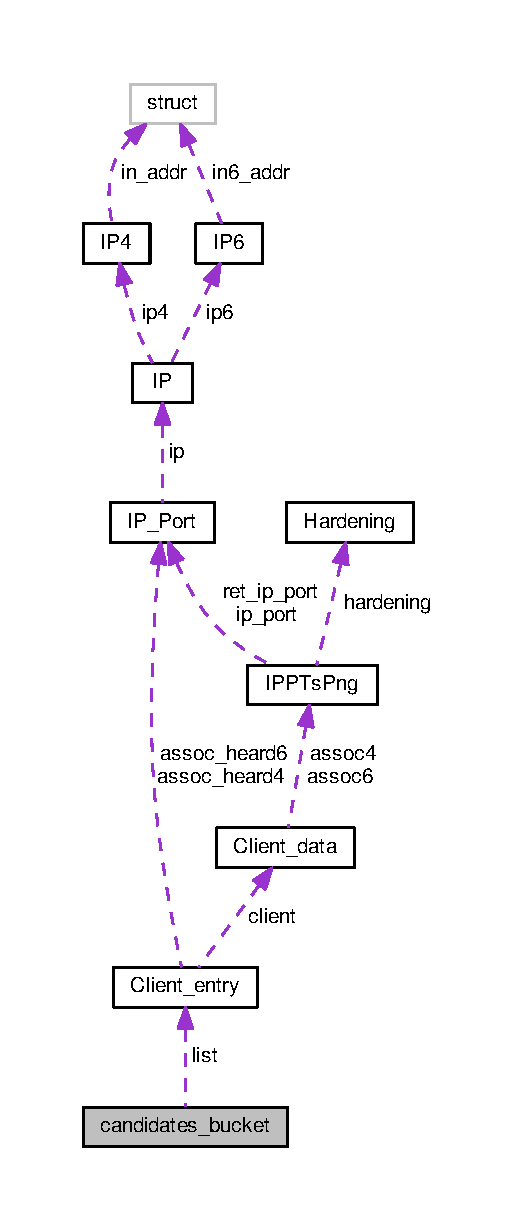
\includegraphics[height=550pt]{d1/d10/structcandidates__bucket__coll__graph}
\end{center}
\end{figure}
\subsection*{Data Fields}
\begin{DoxyCompactItemize}
\item 
\hyperlink{struct_client__entry}{Client\+\_\+entry} $\ast$ \hyperlink{structcandidates__bucket_a515f2b5e53003e623b334ab90c4280e0}{list}
\end{DoxyCompactItemize}


\subsection{Detailed Description}


Definition at line 84 of file assoc.\+c.



\subsection{Field Documentation}
\hypertarget{structcandidates__bucket_a515f2b5e53003e623b334ab90c4280e0}{\index{candidates\+\_\+bucket@{candidates\+\_\+bucket}!list@{list}}
\index{list@{list}!candidates\+\_\+bucket@{candidates\+\_\+bucket}}
\subsubsection[{list}]{\setlength{\rightskip}{0pt plus 5cm}{\bf Client\+\_\+entry}$\ast$ list}}\label{structcandidates__bucket_a515f2b5e53003e623b334ab90c4280e0}


Definition at line 85 of file assoc.\+c.



Referenced by Assoc\+\_\+get\+\_\+close\+\_\+entries(), candidates\+\_\+create\+\_\+internal(), candidates\+\_\+create\+\_\+new(), candidates\+\_\+search(), client\+\_\+id\+\_\+self\+\_\+update(), dist\+\_\+index\+\_\+entry(), do\+\_\+\+Assoc(), kill\+\_\+\+Assoc(), and new\+\_\+\+Assoc().



The documentation for this struct was generated from the following file\+:\begin{DoxyCompactItemize}
\item 
toxcore/\hyperlink{assoc_8c}{assoc.\+c}\end{DoxyCompactItemize}

\hypertarget{struct_client__data}{\section{Client\+\_\+data Struct Reference}
\label{struct_client__data}\index{Client\+\_\+data@{Client\+\_\+data}}
}


Collaboration diagram for Client\+\_\+data\+:
\nopagebreak
\begin{figure}[H]
\begin{center}
\leavevmode
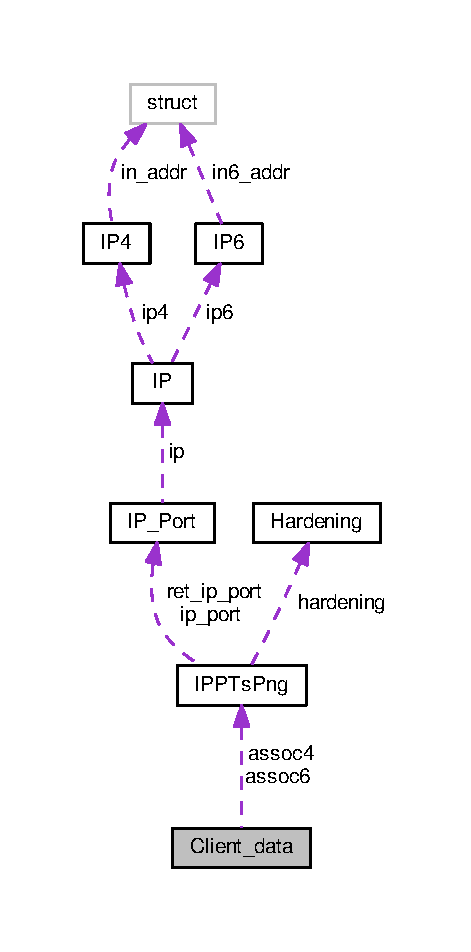
\includegraphics[width=226pt]{struct_client__data__coll__graph}
\end{center}
\end{figure}
\subsection*{Data Fields}
\begin{DoxyCompactItemize}
\item 
\hypertarget{struct_client__data_a72f2085432efcbf0f872298100b06a17}{uint8\+\_\+t {\bfseries client\+\_\+id} \mbox{[}C\+L\+I\+E\+N\+T\+\_\+\+I\+D\+\_\+\+S\+I\+Z\+E\mbox{]}}\label{struct_client__data_a72f2085432efcbf0f872298100b06a17}

\item 
\hypertarget{struct_client__data_ac9843379cbcd02bdfa5c180a1474a6c5}{\hyperlink{struct_i_p_p_ts_png}{I\+P\+P\+Ts\+Png} {\bfseries assoc4}}\label{struct_client__data_ac9843379cbcd02bdfa5c180a1474a6c5}

\item 
\hypertarget{struct_client__data_a87d394929a2604f6f785fec949fac618}{\hyperlink{struct_i_p_p_ts_png}{I\+P\+P\+Ts\+Png} {\bfseries assoc6}}\label{struct_client__data_a87d394929a2604f6f785fec949fac618}

\end{DoxyCompactItemize}


\subsection{Detailed Description}


Definition at line 106 of file D\+H\+T.\+h.



The documentation for this struct was generated from the following file\+:\begin{DoxyCompactItemize}
\item 
toxcore/D\+H\+T.\+h\end{DoxyCompactItemize}

\hypertarget{struct_client__entry}{\section{Client\+\_\+entry Struct Reference}
\label{struct_client__entry}\index{Client\+\_\+entry@{Client\+\_\+entry}}
}


Collaboration diagram for Client\+\_\+entry\+:
\nopagebreak
\begin{figure}[H]
\begin{center}
\leavevmode
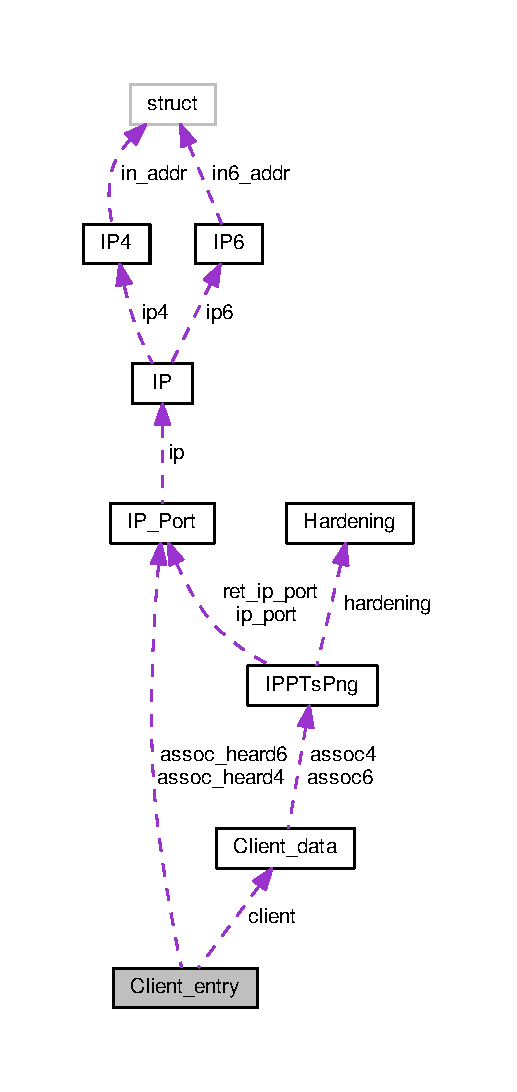
\includegraphics[width=248pt]{struct_client__entry__coll__graph}
\end{center}
\end{figure}
\subsection*{Data Fields}
\begin{DoxyCompactItemize}
\item 
\hypertarget{struct_client__entry_a35aa0f6864b81ef3de3d4d46ef823a0c}{hash\+\_\+t {\bfseries hash}}\label{struct_client__entry_a35aa0f6864b81ef3de3d4d46ef823a0c}

\item 
\hypertarget{struct_client__entry_aec732782691c39a31d8c579a79a8fed2}{uint64\+\_\+t {\bfseries getnodes}}\label{struct_client__entry_aec732782691c39a31d8c579a79a8fed2}

\item 
\hypertarget{struct_client__entry_aa4c583563fdc794eea3b70dcf92870f4}{uint64\+\_\+t {\bfseries used\+\_\+at}}\label{struct_client__entry_aa4c583563fdc794eea3b70dcf92870f4}

\item 
\hypertarget{struct_client__entry_ab632ae1b8a283a06d6cb3881c377c6cd}{uint64\+\_\+t {\bfseries seen\+\_\+at}}\label{struct_client__entry_ab632ae1b8a283a06d6cb3881c377c6cd}

\item 
\hypertarget{struct_client__entry_a0886ba8c555aa6352f2dbf0606636f13}{uint64\+\_\+t {\bfseries heard\+\_\+at}}\label{struct_client__entry_a0886ba8c555aa6352f2dbf0606636f13}

\item 
\hypertarget{struct_client__entry_ac06f60c25b78ef1fce357680b1e5701f}{uint16\+\_\+t {\bfseries seen\+\_\+family}}\label{struct_client__entry_ac06f60c25b78ef1fce357680b1e5701f}

\item 
\hypertarget{struct_client__entry_a1b6b0c24ebf14b86b051d63bd47ffb27}{uint16\+\_\+t {\bfseries heard\+\_\+family}}\label{struct_client__entry_a1b6b0c24ebf14b86b051d63bd47ffb27}

\item 
\hypertarget{struct_client__entry_a85c7d2390e7cf32bb433484f958205f1}{\hyperlink{struct_i_p___port}{I\+P\+\_\+\+Port} {\bfseries assoc\+\_\+heard4}}\label{struct_client__entry_a85c7d2390e7cf32bb433484f958205f1}

\item 
\hypertarget{struct_client__entry_ae6c8f7476cc280c4f1ef1ea4799e728e}{\hyperlink{struct_i_p___port}{I\+P\+\_\+\+Port} {\bfseries assoc\+\_\+heard6}}\label{struct_client__entry_ae6c8f7476cc280c4f1ef1ea4799e728e}

\item 
\hypertarget{struct_client__entry_a114cded03654e9d27771e24fa1712e39}{\hyperlink{struct_client__data}{Client\+\_\+data} {\bfseries client}}\label{struct_client__entry_a114cded03654e9d27771e24fa1712e39}

\end{DoxyCompactItemize}


\subsection{Detailed Description}


Definition at line 65 of file assoc.\+c.



The documentation for this struct was generated from the following file\+:\begin{DoxyCompactItemize}
\item 
toxcore/assoc.\+c\end{DoxyCompactItemize}

\hypertarget{struct_crypto___connection}{\section{Crypto\+\_\+\+Connection Struct Reference}
\label{struct_crypto___connection}\index{Crypto\+\_\+\+Connection@{Crypto\+\_\+\+Connection}}
}


Collaboration diagram for Crypto\+\_\+\+Connection\+:\nopagebreak
\begin{figure}[H]
\begin{center}
\leavevmode
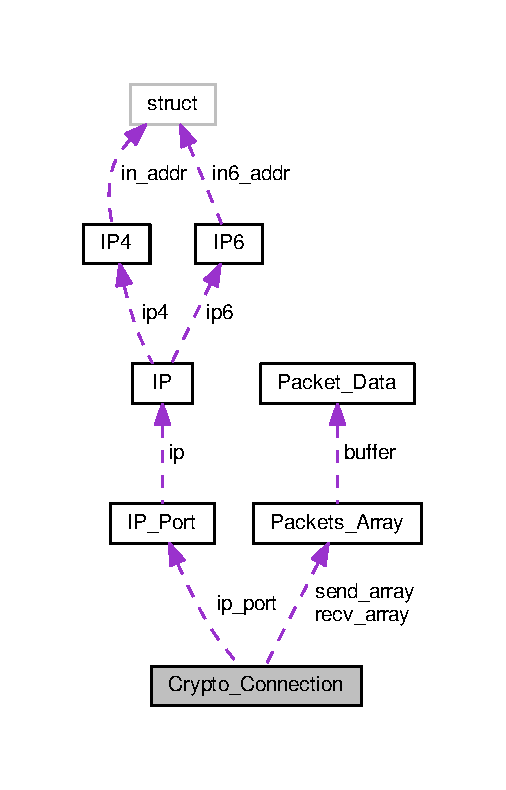
\includegraphics[width=243pt]{struct_crypto___connection__coll__graph}
\end{center}
\end{figure}
\subsection*{Data Fields}
\begin{DoxyCompactItemize}
\item 
\hypertarget{struct_crypto___connection_aaa806bb1136fb3d4b5d8d8970b596ff7}{uint8\+\_\+t {\bfseries public\+\_\+key} \mbox{[}crypto\+\_\+box\+\_\+\+P\+U\+B\+L\+I\+C\+K\+E\+Y\+B\+Y\+T\+E\+S\mbox{]}}\label{struct_crypto___connection_aaa806bb1136fb3d4b5d8d8970b596ff7}

\item 
\hypertarget{struct_crypto___connection_aae0467706f97aa3ef23e5dc9c3c199d7}{uint8\+\_\+t {\bfseries recv\+\_\+nonce} \mbox{[}crypto\+\_\+box\+\_\+\+N\+O\+N\+C\+E\+B\+Y\+T\+E\+S\mbox{]}}\label{struct_crypto___connection_aae0467706f97aa3ef23e5dc9c3c199d7}

\item 
\hypertarget{struct_crypto___connection_a9df0e00e8f493ed6cd1ff45e7da33c0d}{uint8\+\_\+t {\bfseries sent\+\_\+nonce} \mbox{[}crypto\+\_\+box\+\_\+\+N\+O\+N\+C\+E\+B\+Y\+T\+E\+S\mbox{]}}\label{struct_crypto___connection_a9df0e00e8f493ed6cd1ff45e7da33c0d}

\item 
\hypertarget{struct_crypto___connection_a6e74fbae398c7966800ee80f7b93dbfa}{uint8\+\_\+t {\bfseries sessionpublic\+\_\+key} \mbox{[}crypto\+\_\+box\+\_\+\+P\+U\+B\+L\+I\+C\+K\+E\+Y\+B\+Y\+T\+E\+S\mbox{]}}\label{struct_crypto___connection_a6e74fbae398c7966800ee80f7b93dbfa}

\item 
\hypertarget{struct_crypto___connection_a5f38fc9ff1b20b61ffbb56d9e7f5c892}{uint8\+\_\+t {\bfseries sessionsecret\+\_\+key} \mbox{[}crypto\+\_\+box\+\_\+\+S\+E\+C\+R\+E\+T\+K\+E\+Y\+B\+Y\+T\+E\+S\mbox{]}}\label{struct_crypto___connection_a5f38fc9ff1b20b61ffbb56d9e7f5c892}

\item 
\hypertarget{struct_crypto___connection_ac040d4ba2a22ee327952009e7396bb2f}{uint8\+\_\+t {\bfseries peersessionpublic\+\_\+key} \mbox{[}crypto\+\_\+box\+\_\+\+P\+U\+B\+L\+I\+C\+K\+E\+Y\+B\+Y\+T\+E\+S\mbox{]}}\label{struct_crypto___connection_ac040d4ba2a22ee327952009e7396bb2f}

\item 
\hypertarget{struct_crypto___connection_a81ead9fac55a0cedc30a96253a2c5119}{uint8\+\_\+t {\bfseries shared\+\_\+key} \mbox{[}crypto\+\_\+box\+\_\+\+B\+E\+F\+O\+R\+E\+N\+M\+B\+Y\+T\+E\+S\mbox{]}}\label{struct_crypto___connection_a81ead9fac55a0cedc30a96253a2c5119}

\item 
\hypertarget{struct_crypto___connection_ade818037fd6c985038ff29656089758d}{uint8\+\_\+t {\bfseries status}}\label{struct_crypto___connection_ade818037fd6c985038ff29656089758d}

\item 
\hypertarget{struct_crypto___connection_acb77d5443961bf245b63c17347b1b030}{uint64\+\_\+t {\bfseries cookie\+\_\+request\+\_\+number}}\label{struct_crypto___connection_acb77d5443961bf245b63c17347b1b030}

\item 
\hypertarget{struct_crypto___connection_ab2ecaa07625ad0ed5e07d3a1f0dcc939}{uint8\+\_\+t {\bfseries dht\+\_\+public\+\_\+key} \mbox{[}crypto\+\_\+box\+\_\+\+P\+U\+B\+L\+I\+C\+K\+E\+Y\+B\+Y\+T\+E\+S\mbox{]}}\label{struct_crypto___connection_ab2ecaa07625ad0ed5e07d3a1f0dcc939}

\item 
\hypertarget{struct_crypto___connection_a360adb14f743065d5c69fe29a00a06a7}{uint8\+\_\+t $\ast$ {\bfseries temp\+\_\+packet}}\label{struct_crypto___connection_a360adb14f743065d5c69fe29a00a06a7}

\item 
\hypertarget{struct_crypto___connection_a4ef842580c6c073f36578d0e07551cc4}{uint16\+\_\+t {\bfseries temp\+\_\+packet\+\_\+length}}\label{struct_crypto___connection_a4ef842580c6c073f36578d0e07551cc4}

\item 
\hypertarget{struct_crypto___connection_abb5fdaef769d667f90bc97bd72d765d6}{uint64\+\_\+t {\bfseries temp\+\_\+packet\+\_\+sent\+\_\+time}}\label{struct_crypto___connection_abb5fdaef769d667f90bc97bd72d765d6}

\item 
\hypertarget{struct_crypto___connection_a7386b7ad7bedb9dd47d898f588b4f463}{uint32\+\_\+t {\bfseries temp\+\_\+packet\+\_\+num\+\_\+sent}}\label{struct_crypto___connection_a7386b7ad7bedb9dd47d898f588b4f463}

\item 
\hypertarget{struct_crypto___connection_a86e2a5a56c0dd22df6e8b8a10e40f9e4}{\hyperlink{struct_i_p___port}{I\+P\+\_\+\+Port} {\bfseries ip\+\_\+port}}\label{struct_crypto___connection_a86e2a5a56c0dd22df6e8b8a10e40f9e4}

\item 
\hypertarget{struct_crypto___connection_ac6eb8a274b0dedea83359f2d9269cbc2}{uint64\+\_\+t {\bfseries direct\+\_\+lastrecv\+\_\+time}}\label{struct_crypto___connection_ac6eb8a274b0dedea83359f2d9269cbc2}

\item 
\hypertarget{struct_crypto___connection_aa9112ee7e76eb3e870491f7c5c272197}{\hyperlink{struct_packets___array}{Packets\+\_\+\+Array} {\bfseries send\+\_\+array}}\label{struct_crypto___connection_aa9112ee7e76eb3e870491f7c5c272197}

\item 
\hypertarget{struct_crypto___connection_a1a62bc0c4bb9e349735c65f9948020d5}{\hyperlink{struct_packets___array}{Packets\+\_\+\+Array} {\bfseries recv\+\_\+array}}\label{struct_crypto___connection_a1a62bc0c4bb9e349735c65f9948020d5}

\item 
\hypertarget{struct_crypto___connection_ad3c663c15ca97b75951ea711b522c049}{int($\ast$ {\bfseries connection\+\_\+status\+\_\+callback} )(void $\ast$object, int id, uint8\+\_\+t status)}\label{struct_crypto___connection_ad3c663c15ca97b75951ea711b522c049}

\item 
\hypertarget{struct_crypto___connection_afe03d43c62ac2aa575a39e4308353244}{void $\ast$ {\bfseries connection\+\_\+status\+\_\+callback\+\_\+object}}\label{struct_crypto___connection_afe03d43c62ac2aa575a39e4308353244}

\item 
\hypertarget{struct_crypto___connection_a3cd6f7015115dc493f86be91526eb9f8}{int {\bfseries connection\+\_\+status\+\_\+callback\+\_\+id}}\label{struct_crypto___connection_a3cd6f7015115dc493f86be91526eb9f8}

\item 
\hypertarget{struct_crypto___connection_adc6ee264e4a5758049c6299beb81ce6d}{int($\ast$ {\bfseries connection\+\_\+data\+\_\+callback} )(void $\ast$object, int id, uint8\+\_\+t $\ast$data, uint16\+\_\+t length)}\label{struct_crypto___connection_adc6ee264e4a5758049c6299beb81ce6d}

\item 
\hypertarget{struct_crypto___connection_a3c44dfac7528ae10a6d09bf812f36486}{void $\ast$ {\bfseries connection\+\_\+data\+\_\+callback\+\_\+object}}\label{struct_crypto___connection_a3c44dfac7528ae10a6d09bf812f36486}

\item 
\hypertarget{struct_crypto___connection_a7d50567cce6cb1b8ef983e64060d414e}{int {\bfseries connection\+\_\+data\+\_\+callback\+\_\+id}}\label{struct_crypto___connection_a7d50567cce6cb1b8ef983e64060d414e}

\item 
\hypertarget{struct_crypto___connection_ab5af8aad05ddc085e69ead928cc26313}{int($\ast$ {\bfseries connection\+\_\+lossy\+\_\+data\+\_\+callback} )(void $\ast$object, int id, const uint8\+\_\+t $\ast$data, uint16\+\_\+t length)}\label{struct_crypto___connection_ab5af8aad05ddc085e69ead928cc26313}

\item 
\hypertarget{struct_crypto___connection_a70a99b7d0c9dd2f913ca9ea42bafc942}{void $\ast$ {\bfseries connection\+\_\+lossy\+\_\+data\+\_\+callback\+\_\+object}}\label{struct_crypto___connection_a70a99b7d0c9dd2f913ca9ea42bafc942}

\item 
\hypertarget{struct_crypto___connection_acdd49847729119bc5d6cc7269cde876a}{int {\bfseries connection\+\_\+lossy\+\_\+data\+\_\+callback\+\_\+id}}\label{struct_crypto___connection_acdd49847729119bc5d6cc7269cde876a}

\item 
\hypertarget{struct_crypto___connection_aa0c15e9ada39b9e8d1f27e2a10ad2e0e}{uint64\+\_\+t {\bfseries last\+\_\+request\+\_\+packet\+\_\+sent}}\label{struct_crypto___connection_aa0c15e9ada39b9e8d1f27e2a10ad2e0e}

\item 
\hypertarget{struct_crypto___connection_a253e0640ca1d914e479ea37e97d1ba12}{uint32\+\_\+t {\bfseries packet\+\_\+counter}}\label{struct_crypto___connection_a253e0640ca1d914e479ea37e97d1ba12}

\item 
\hypertarget{struct_crypto___connection_ae1c1fa0c995f0fab590b094baa769e8d}{double {\bfseries packet\+\_\+recv\+\_\+rate}}\label{struct_crypto___connection_ae1c1fa0c995f0fab590b094baa769e8d}

\item 
\hypertarget{struct_crypto___connection_a77c1105a8f0d4de4daab379a572bb11c}{uint64\+\_\+t {\bfseries packet\+\_\+counter\+\_\+set}}\label{struct_crypto___connection_a77c1105a8f0d4de4daab379a572bb11c}

\item 
\hypertarget{struct_crypto___connection_a8358768a02871910ed059b1b2646438e}{double {\bfseries packet\+\_\+send\+\_\+rate}}\label{struct_crypto___connection_a8358768a02871910ed059b1b2646438e}

\item 
\hypertarget{struct_crypto___connection_adfabcbe80305cc6b4e1c0dfef5c48653}{uint32\+\_\+t {\bfseries packets\+\_\+left}}\label{struct_crypto___connection_adfabcbe80305cc6b4e1c0dfef5c48653}

\item 
\hypertarget{struct_crypto___connection_a3c50560fad9a00689d5d3f143f4b56aa}{uint64\+\_\+t {\bfseries last\+\_\+packets\+\_\+left\+\_\+set}}\label{struct_crypto___connection_a3c50560fad9a00689d5d3f143f4b56aa}

\item 
\hypertarget{struct_crypto___connection_a0157f7d2fcd3f9d92521930547ddaae6}{uint32\+\_\+t {\bfseries last\+\_\+sendqueue\+\_\+size} \mbox{[}C\+O\+N\+G\+E\+S\+T\+I\+O\+N\+\_\+\+Q\+U\+E\+U\+E\+\_\+\+A\+R\+R\+A\+Y\+\_\+\+S\+I\+Z\+E\mbox{]}}\label{struct_crypto___connection_a0157f7d2fcd3f9d92521930547ddaae6}

\item 
\hypertarget{struct_crypto___connection_a9fff7889476ca9104b603dd03781e0c9}{uint32\+\_\+t {\bfseries last\+\_\+sendqueue\+\_\+counter}}\label{struct_crypto___connection_a9fff7889476ca9104b603dd03781e0c9}

\item 
\hypertarget{struct_crypto___connection_aa6d1d107adcffe30564bf3837faefca4}{long signed int {\bfseries last\+\_\+num\+\_\+packets\+\_\+sent} \mbox{[}C\+O\+N\+G\+E\+S\+T\+I\+O\+N\+\_\+\+Q\+U\+E\+U\+E\+\_\+\+A\+R\+R\+A\+Y\+\_\+\+S\+I\+Z\+E\mbox{]}}\label{struct_crypto___connection_aa6d1d107adcffe30564bf3837faefca4}

\item 
\hypertarget{struct_crypto___connection_ad51d37ac38989c1d089da8aa0d1bc1d7}{uint32\+\_\+t {\bfseries packets\+\_\+sent}}\label{struct_crypto___connection_ad51d37ac38989c1d089da8aa0d1bc1d7}

\item 
\hypertarget{struct_crypto___connection_ad33f09e937800c05f22fa695e756554d}{uint64\+\_\+t {\bfseries last\+\_\+congestion\+\_\+event}}\label{struct_crypto___connection_ad33f09e937800c05f22fa695e756554d}

\item 
\hypertarget{struct_crypto___connection_ae88ec876060fbc648a4c75ac596137f9}{uint64\+\_\+t {\bfseries rtt\+\_\+time}}\label{struct_crypto___connection_ae88ec876060fbc648a4c75ac596137f9}

\item 
\hypertarget{struct_crypto___connection_a51666aaba0fc5680040fe5bd6778bc50}{unsigned int {\bfseries connection\+\_\+number\+\_\+tcp}}\label{struct_crypto___connection_a51666aaba0fc5680040fe5bd6778bc50}

\item 
\hypertarget{struct_crypto___connection_a8aa9d51e0fa27ad34f8046486d519275}{uint8\+\_\+t {\bfseries maximum\+\_\+speed\+\_\+reached}}\label{struct_crypto___connection_a8aa9d51e0fa27ad34f8046486d519275}

\item 
\hypertarget{struct_crypto___connection_a4acff8232e4aec9cd5c6dc200ac55ef3}{pthread\+\_\+mutex\+\_\+t {\bfseries mutex}}\label{struct_crypto___connection_a4acff8232e4aec9cd5c6dc200ac55ef3}

\item 
\hypertarget{struct_crypto___connection_ab0f780a41ece58bf84d8460e71cbdbb3}{void($\ast$ {\bfseries dht\+\_\+pk\+\_\+callback} )(void $\ast$data, int32\+\_\+t number, const uint8\+\_\+t $\ast$dht\+\_\+public\+\_\+key)}\label{struct_crypto___connection_ab0f780a41ece58bf84d8460e71cbdbb3}

\item 
\hypertarget{struct_crypto___connection_ab5d618d73b8d83fb07209433e7b448ee}{void $\ast$ {\bfseries dht\+\_\+pk\+\_\+callback\+\_\+object}}\label{struct_crypto___connection_ab5d618d73b8d83fb07209433e7b448ee}

\item 
\hypertarget{struct_crypto___connection_ab0413da421baacf312141b8ae3ec7762}{uint32\+\_\+t {\bfseries dht\+\_\+pk\+\_\+callback\+\_\+number}}\label{struct_crypto___connection_ab0413da421baacf312141b8ae3ec7762}

\end{DoxyCompactItemize}


\subsection{Detailed Description}


Definition at line 100 of file net\+\_\+crypto.\+h.



The documentation for this struct was generated from the following file\+:\begin{DoxyCompactItemize}
\item 
toxcore/net\+\_\+crypto.\+h\end{DoxyCompactItemize}

\hypertarget{struct_cryptopacket___handles}{\section{Cryptopacket\+\_\+\+Handles Struct Reference}
\label{struct_cryptopacket___handles}\index{Cryptopacket\+\_\+\+Handles@{Cryptopacket\+\_\+\+Handles}}
}


Collaboration diagram for Cryptopacket\+\_\+\+Handles\+:
\nopagebreak
\begin{figure}[H]
\begin{center}
\leavevmode
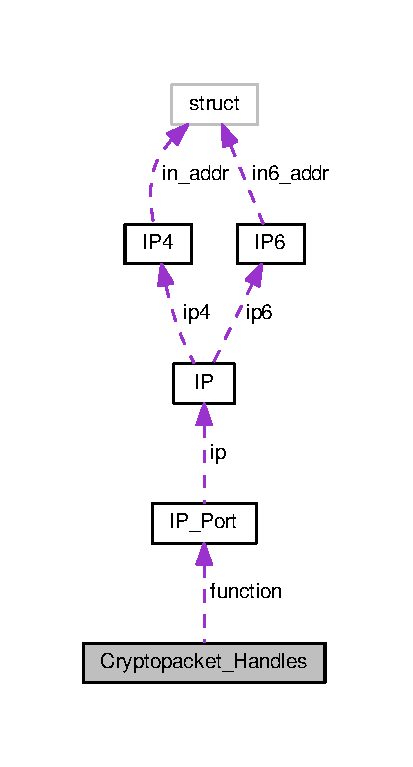
\includegraphics[width=198pt]{struct_cryptopacket___handles__coll__graph}
\end{center}
\end{figure}
\subsection*{Data Fields}
\begin{DoxyCompactItemize}
\item 
\hypertarget{struct_cryptopacket___handles_a9313784040f9666743d9aff915543903}{cryptopacket\+\_\+handler\+\_\+callback {\bfseries function}}\label{struct_cryptopacket___handles_a9313784040f9666743d9aff915543903}

\item 
\hypertarget{struct_cryptopacket___handles_a077376d12464f945e2414d5499c79b3f}{void $\ast$ {\bfseries object}}\label{struct_cryptopacket___handles_a077376d12464f945e2414d5499c79b3f}

\end{DoxyCompactItemize}


\subsection{Detailed Description}


Definition at line 193 of file D\+H\+T.\+h.



The documentation for this struct was generated from the following file\+:\begin{DoxyCompactItemize}
\item 
toxcore/D\+H\+T.\+h\end{DoxyCompactItemize}

\hypertarget{struct_d_h_t}{\section{D\+H\+T Struct Reference}
\label{struct_d_h_t}\index{D\+H\+T@{D\+H\+T}}
}


{\ttfamily \#include $<$D\+H\+T.\+h$>$}



Collaboration diagram for D\+H\+T\+:
\nopagebreak
\begin{figure}[H]
\begin{center}
\leavevmode
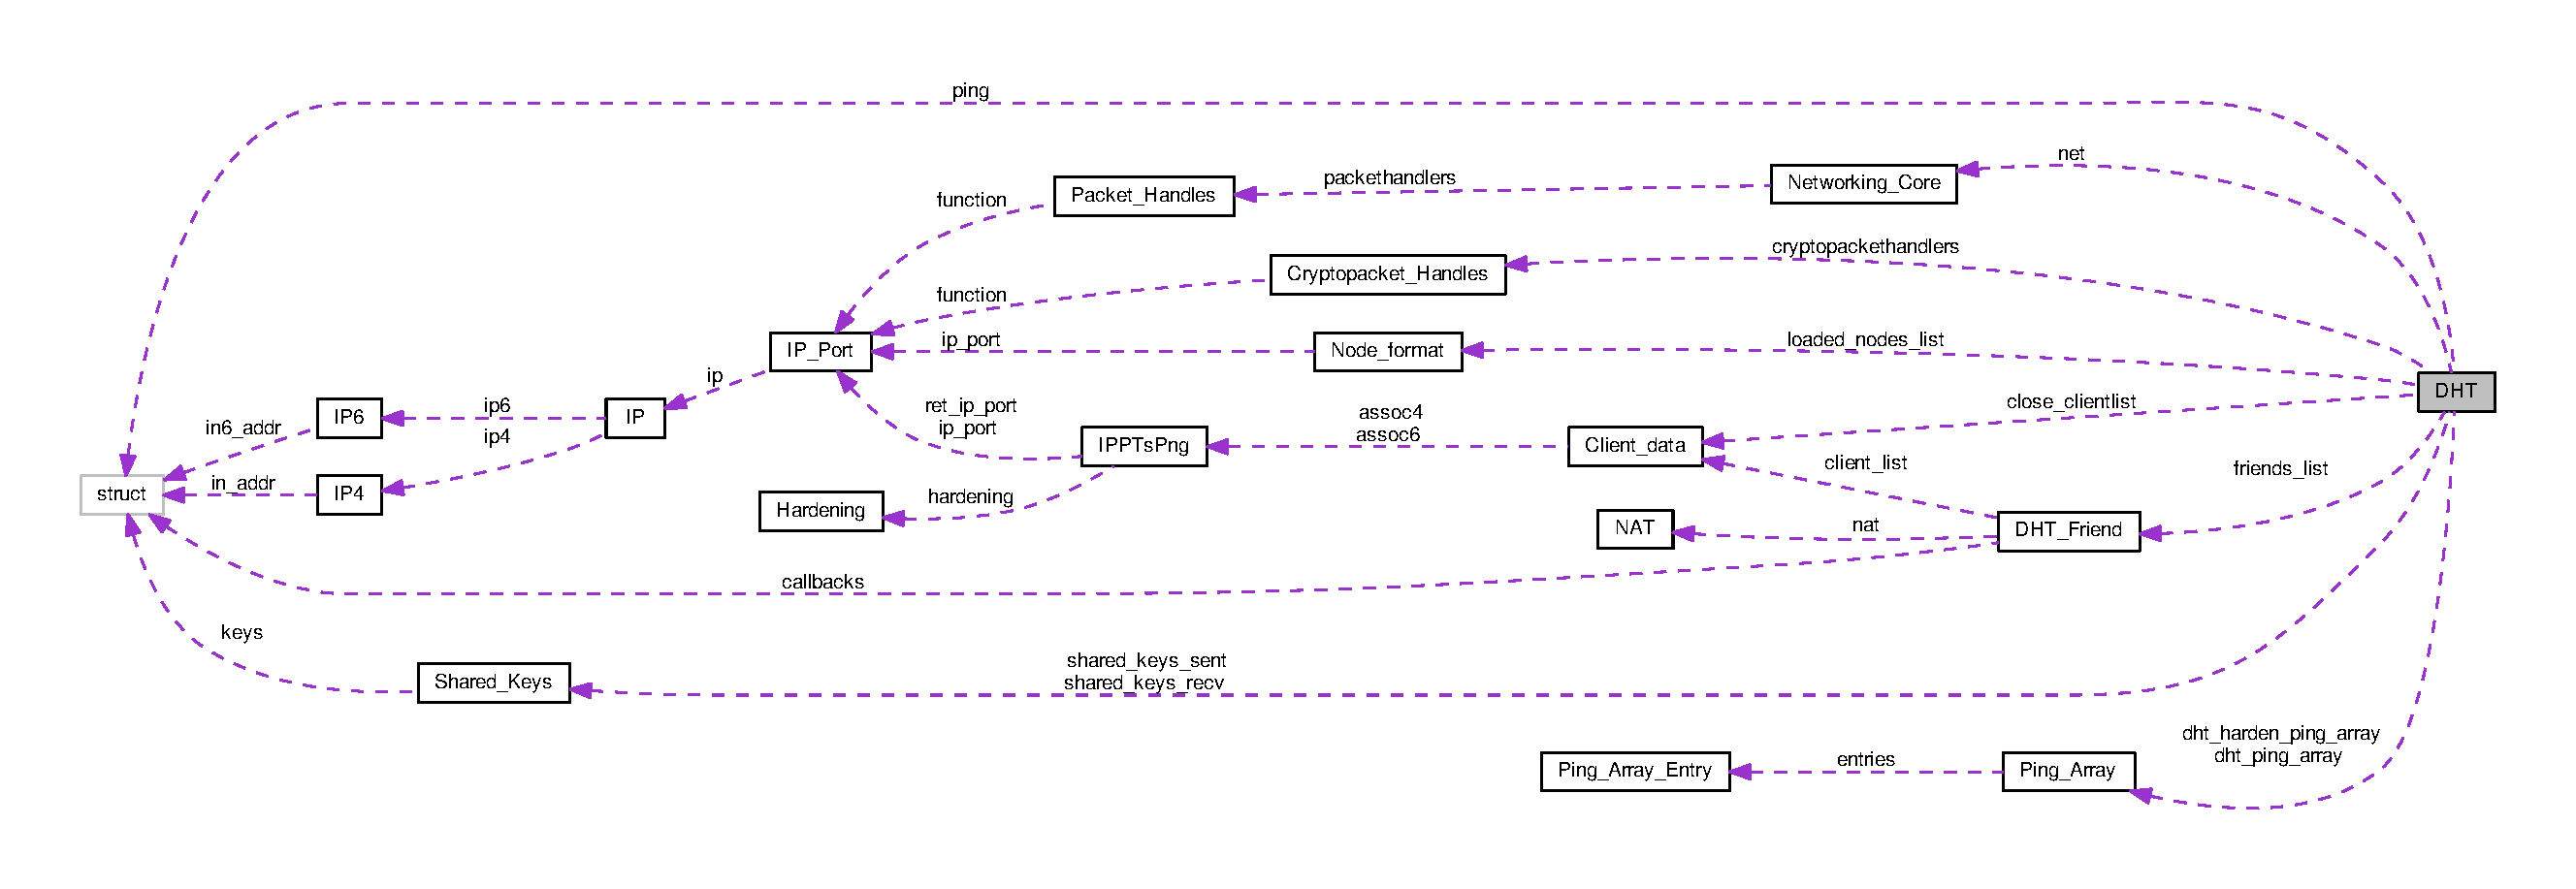
\includegraphics[width=350pt]{d9/d93/struct_d_h_t__coll__graph}
\end{center}
\end{figure}
\subsection*{Data Fields}
\begin{DoxyCompactItemize}
\item 
\hyperlink{struct_networking___core}{Networking\+\_\+\+Core} $\ast$ \hyperlink{struct_d_h_t_aa14ea2f67950f57fe4235d7375a2216c}{net}
\item 
\hyperlink{struct_client__data}{Client\+\_\+data} \hyperlink{struct_d_h_t_a00ef35d5b0e7a791ef08a30b3bacbf9d}{close\+\_\+clientlist} \mbox{[}\hyperlink{_d_h_t_8h_a3058f857a8316099e20c95fb07adc7c1}{L\+C\+L\+I\+E\+N\+T\+\_\+\+L\+I\+S\+T}\mbox{]}
\item 
uint64\+\_\+t \hyperlink{struct_d_h_t_a3ab563f182d86c5bc6322ee416a10a32}{close\+\_\+lastgetnodes}
\item 
uint32\+\_\+t \hyperlink{struct_d_h_t_afacccecf0d2090a9dec8d06f3f119087}{close\+\_\+bootstrap\+\_\+times}
\item 
uint8\+\_\+t \hyperlink{struct_d_h_t_ab9f2ff47bc0b1e5110202a6e4be86390}{secret\+\_\+symmetric\+\_\+key} \mbox{[}\hyperlink{crypto__core_8h_aade7cd33abc5668970c55ed009ab00c8}{crypto\+\_\+box\+\_\+\+K\+E\+Y\+B\+Y\+T\+E\+S}\mbox{]}
\item 
uint8\+\_\+t \hyperlink{struct_d_h_t_ae726df8bdc26380e5a6c3187a00d6881}{self\+\_\+public\+\_\+key} \mbox{[}crypto\+\_\+box\+\_\+\+P\+U\+B\+L\+I\+C\+K\+E\+Y\+B\+Y\+T\+E\+S\mbox{]}
\item 
uint8\+\_\+t \hyperlink{struct_d_h_t_aa05050f86513ff53fe9da81f73c72267}{self\+\_\+secret\+\_\+key} \mbox{[}crypto\+\_\+box\+\_\+\+S\+E\+C\+R\+E\+T\+K\+E\+Y\+B\+Y\+T\+E\+S\mbox{]}
\item 
\hyperlink{struct_d_h_t___friend}{D\+H\+T\+\_\+\+Friend} $\ast$ \hyperlink{struct_d_h_t_ae97c6b057d770e7c4f3905cbe33b188b}{friends\+\_\+list}
\item 
uint16\+\_\+t \hyperlink{struct_d_h_t_a8ee1f2d7e543bce350c591a8eaac0cf8}{num\+\_\+friends}
\item 
\hyperlink{struct_node__format}{Node\+\_\+format} $\ast$ \hyperlink{struct_d_h_t_a3050c21873637c51d8001c807f62fa74}{loaded\+\_\+nodes\+\_\+list}
\item 
uint32\+\_\+t \hyperlink{struct_d_h_t_aef4ce67d5df5f093247c73b3a024b73e}{loaded\+\_\+num\+\_\+nodes}
\item 
unsigned int \hyperlink{struct_d_h_t_a6525da58097b462adbe2ad9000a6d77d}{loaded\+\_\+nodes\+\_\+index}
\item 
\hyperlink{struct_shared___keys}{Shared\+\_\+\+Keys} \hyperlink{struct_d_h_t_a4c647e235c4b9d2d6d68d760c7cb1b30}{shared\+\_\+keys\+\_\+recv}
\item 
\hyperlink{struct_shared___keys}{Shared\+\_\+\+Keys} \hyperlink{struct_d_h_t_a07b2f51891b851ec0cd7dfe729412f77}{shared\+\_\+keys\+\_\+sent}
\item 
struct \hyperlink{struct_p_i_n_g}{P\+I\+N\+G} $\ast$ \hyperlink{struct_d_h_t_ae3f68e3d55e46726b05717fc88198321}{ping}
\item 
\hyperlink{struct_ping___array}{Ping\+\_\+\+Array} \hyperlink{struct_d_h_t_a8432234ba71a00ac9c516cb80a70f29d}{dht\+\_\+ping\+\_\+array}
\item 
\hyperlink{struct_ping___array}{Ping\+\_\+\+Array} \hyperlink{struct_d_h_t_a957126e184a8b8001228effc56b9db95}{dht\+\_\+harden\+\_\+ping\+\_\+array}
\item 
uint64\+\_\+t \hyperlink{struct_d_h_t_a73e8197b772061572cb931a378ade3e4}{last\+\_\+run}
\item 
\hyperlink{struct_cryptopacket___handles}{Cryptopacket\+\_\+\+Handles} \hyperlink{struct_d_h_t_a461ccd9a581712b103785034f31d0d82}{cryptopackethandlers} \mbox{[}256\mbox{]}
\end{DoxyCompactItemize}


\subsection{Detailed Description}


Definition at line 200 of file D\+H\+T.\+h.



\subsection{Field Documentation}
\hypertarget{struct_d_h_t_afacccecf0d2090a9dec8d06f3f119087}{\index{D\+H\+T@{D\+H\+T}!close\+\_\+bootstrap\+\_\+times@{close\+\_\+bootstrap\+\_\+times}}
\index{close\+\_\+bootstrap\+\_\+times@{close\+\_\+bootstrap\+\_\+times}!D\+H\+T@{D\+H\+T}}
\subsubsection[{close\+\_\+bootstrap\+\_\+times}]{\setlength{\rightskip}{0pt plus 5cm}uint32\+\_\+t close\+\_\+bootstrap\+\_\+times}}\label{struct_d_h_t_afacccecf0d2090a9dec8d06f3f119087}


Definition at line 205 of file D\+H\+T.\+h.



Referenced by do\+\_\+\+Close().

\hypertarget{struct_d_h_t_a00ef35d5b0e7a791ef08a30b3bacbf9d}{\index{D\+H\+T@{D\+H\+T}!close\+\_\+clientlist@{close\+\_\+clientlist}}
\index{close\+\_\+clientlist@{close\+\_\+clientlist}!D\+H\+T@{D\+H\+T}}
\subsubsection[{close\+\_\+clientlist}]{\setlength{\rightskip}{0pt plus 5cm}{\bf Client\+\_\+data} close\+\_\+clientlist\mbox{[}{\bf L\+C\+L\+I\+E\+N\+T\+\_\+\+L\+I\+S\+T}\mbox{]}}}\label{struct_d_h_t_a00ef35d5b0e7a791ef08a30b3bacbf9d}


Definition at line 203 of file D\+H\+T.\+h.



Referenced by add\+\_\+to\+\_\+ping(), addto\+\_\+lists(), closelist\+\_\+nodes(), D\+H\+T\+\_\+isconnected(), D\+H\+T\+\_\+non\+\_\+lan\+\_\+connected(), D\+H\+T\+\_\+save(), D\+H\+T\+\_\+size(), do\+\_\+\+Close(), do\+\_\+hardening(), do\+\_\+messenger(), get\+\_\+closelist\+\_\+\+I\+P\+P\+Ts\+Png(), get\+\_\+somewhat\+\_\+close\+\_\+nodes(), ping\+\_\+node\+\_\+from\+\_\+getnodes\+\_\+ok(), print\+\_\+clientlist(), returnedip\+\_\+ports(), route\+\_\+packet(), and test\+\_\+addto\+\_\+lists().

\hypertarget{struct_d_h_t_a3ab563f182d86c5bc6322ee416a10a32}{\index{D\+H\+T@{D\+H\+T}!close\+\_\+lastgetnodes@{close\+\_\+lastgetnodes}}
\index{close\+\_\+lastgetnodes@{close\+\_\+lastgetnodes}!D\+H\+T@{D\+H\+T}}
\subsubsection[{close\+\_\+lastgetnodes}]{\setlength{\rightskip}{0pt plus 5cm}uint64\+\_\+t close\+\_\+lastgetnodes}}\label{struct_d_h_t_a3ab563f182d86c5bc6322ee416a10a32}


Definition at line 204 of file D\+H\+T.\+h.



Referenced by do\+\_\+\+Close().

\hypertarget{struct_d_h_t_a461ccd9a581712b103785034f31d0d82}{\index{D\+H\+T@{D\+H\+T}!cryptopackethandlers@{cryptopackethandlers}}
\index{cryptopackethandlers@{cryptopackethandlers}!D\+H\+T@{D\+H\+T}}
\subsubsection[{cryptopackethandlers}]{\setlength{\rightskip}{0pt plus 5cm}{\bf Cryptopacket\+\_\+\+Handles} cryptopackethandlers\mbox{[}256\mbox{]}}}\label{struct_d_h_t_a461ccd9a581712b103785034f31d0d82}


Definition at line 231 of file D\+H\+T.\+h.



Referenced by cryptopacket\+\_\+handle(), and cryptopacket\+\_\+registerhandler().

\hypertarget{struct_d_h_t_a957126e184a8b8001228effc56b9db95}{\index{D\+H\+T@{D\+H\+T}!dht\+\_\+harden\+\_\+ping\+\_\+array@{dht\+\_\+harden\+\_\+ping\+\_\+array}}
\index{dht\+\_\+harden\+\_\+ping\+\_\+array@{dht\+\_\+harden\+\_\+ping\+\_\+array}!D\+H\+T@{D\+H\+T}}
\subsubsection[{dht\+\_\+harden\+\_\+ping\+\_\+array}]{\setlength{\rightskip}{0pt plus 5cm}{\bf Ping\+\_\+\+Array} dht\+\_\+harden\+\_\+ping\+\_\+array}}\label{struct_d_h_t_a957126e184a8b8001228effc56b9db95}


Definition at line 225 of file D\+H\+T.\+h.



Referenced by getnodes(), kill\+\_\+\+D\+H\+T(), new\+\_\+\+D\+H\+T(), and sent\+\_\+getnode\+\_\+to\+\_\+node().

\hypertarget{struct_d_h_t_a8432234ba71a00ac9c516cb80a70f29d}{\index{D\+H\+T@{D\+H\+T}!dht\+\_\+ping\+\_\+array@{dht\+\_\+ping\+\_\+array}}
\index{dht\+\_\+ping\+\_\+array@{dht\+\_\+ping\+\_\+array}!D\+H\+T@{D\+H\+T}}
\subsubsection[{dht\+\_\+ping\+\_\+array}]{\setlength{\rightskip}{0pt plus 5cm}{\bf Ping\+\_\+\+Array} dht\+\_\+ping\+\_\+array}}\label{struct_d_h_t_a8432234ba71a00ac9c516cb80a70f29d}


Definition at line 224 of file D\+H\+T.\+h.



Referenced by getnodes(), kill\+\_\+\+D\+H\+T(), new\+\_\+\+D\+H\+T(), and sent\+\_\+getnode\+\_\+to\+\_\+node().

\hypertarget{struct_d_h_t_ae97c6b057d770e7c4f3905cbe33b188b}{\index{D\+H\+T@{D\+H\+T}!friends\+\_\+list@{friends\+\_\+list}}
\index{friends\+\_\+list@{friends\+\_\+list}!D\+H\+T@{D\+H\+T}}
\subsubsection[{friends\+\_\+list}]{\setlength{\rightskip}{0pt plus 5cm}{\bf D\+H\+T\+\_\+\+Friend}$\ast$ friends\+\_\+list}}\label{struct_d_h_t_ae97c6b057d770e7c4f3905cbe33b188b}


Definition at line 213 of file D\+H\+T.\+h.



Referenced by addto\+\_\+lists(), D\+H\+T\+\_\+addfriend(), D\+H\+T\+\_\+delfriend(), D\+H\+T\+\_\+getfriendip(), D\+H\+T\+\_\+save(), D\+H\+T\+\_\+size(), do\+\_\+\+D\+H\+T\+\_\+friends(), do\+\_\+messenger(), do\+\_\+\+N\+A\+T(), friend\+\_\+iplist(), friend\+\_\+number(), get\+\_\+somewhat\+\_\+close\+\_\+nodes(), handle\+\_\+\+N\+A\+Tping(), kill\+\_\+\+D\+H\+T(), ping\+\_\+node\+\_\+from\+\_\+getnodes\+\_\+ok(), print\+\_\+friendlist(), punch\+\_\+holes(), returnedip\+\_\+ports(), route\+\_\+tofriend(), routeone\+\_\+tofriend(), and test\+\_\+addto\+\_\+lists().

\hypertarget{struct_d_h_t_a73e8197b772061572cb931a378ade3e4}{\index{D\+H\+T@{D\+H\+T}!last\+\_\+run@{last\+\_\+run}}
\index{last\+\_\+run@{last\+\_\+run}!D\+H\+T@{D\+H\+T}}
\subsubsection[{last\+\_\+run}]{\setlength{\rightskip}{0pt plus 5cm}uint64\+\_\+t last\+\_\+run}}\label{struct_d_h_t_a73e8197b772061572cb931a378ade3e4}


Definition at line 229 of file D\+H\+T.\+h.



Referenced by do\+\_\+\+D\+H\+T().

\hypertarget{struct_d_h_t_a6525da58097b462adbe2ad9000a6d77d}{\index{D\+H\+T@{D\+H\+T}!loaded\+\_\+nodes\+\_\+index@{loaded\+\_\+nodes\+\_\+index}}
\index{loaded\+\_\+nodes\+\_\+index@{loaded\+\_\+nodes\+\_\+index}!D\+H\+T@{D\+H\+T}}
\subsubsection[{loaded\+\_\+nodes\+\_\+index}]{\setlength{\rightskip}{0pt plus 5cm}unsigned int loaded\+\_\+nodes\+\_\+index}}\label{struct_d_h_t_a6525da58097b462adbe2ad9000a6d77d}


Definition at line 218 of file D\+H\+T.\+h.



Referenced by D\+H\+T\+\_\+connect\+\_\+after\+\_\+load().

\hypertarget{struct_d_h_t_a3050c21873637c51d8001c807f62fa74}{\index{D\+H\+T@{D\+H\+T}!loaded\+\_\+nodes\+\_\+list@{loaded\+\_\+nodes\+\_\+list}}
\index{loaded\+\_\+nodes\+\_\+list@{loaded\+\_\+nodes\+\_\+list}!D\+H\+T@{D\+H\+T}}
\subsubsection[{loaded\+\_\+nodes\+\_\+list}]{\setlength{\rightskip}{0pt plus 5cm}{\bf Node\+\_\+format}$\ast$ loaded\+\_\+nodes\+\_\+list}}\label{struct_d_h_t_a3050c21873637c51d8001c807f62fa74}


Definition at line 216 of file D\+H\+T.\+h.



Referenced by D\+H\+T\+\_\+connect\+\_\+after\+\_\+load(), dht\+\_\+load\+\_\+state\+\_\+callback(), and kill\+\_\+\+D\+H\+T().

\hypertarget{struct_d_h_t_aef4ce67d5df5f093247c73b3a024b73e}{\index{D\+H\+T@{D\+H\+T}!loaded\+\_\+num\+\_\+nodes@{loaded\+\_\+num\+\_\+nodes}}
\index{loaded\+\_\+num\+\_\+nodes@{loaded\+\_\+num\+\_\+nodes}!D\+H\+T@{D\+H\+T}}
\subsubsection[{loaded\+\_\+num\+\_\+nodes}]{\setlength{\rightskip}{0pt plus 5cm}uint32\+\_\+t loaded\+\_\+num\+\_\+nodes}}\label{struct_d_h_t_aef4ce67d5df5f093247c73b3a024b73e}


Definition at line 217 of file D\+H\+T.\+h.



Referenced by D\+H\+T\+\_\+connect\+\_\+after\+\_\+load(), dht\+\_\+load\+\_\+state\+\_\+callback(), and do\+\_\+\+D\+H\+T().

\hypertarget{struct_d_h_t_aa14ea2f67950f57fe4235d7375a2216c}{\index{D\+H\+T@{D\+H\+T}!net@{net}}
\index{net@{net}!D\+H\+T@{D\+H\+T}}
\subsubsection[{net}]{\setlength{\rightskip}{0pt plus 5cm}{\bf Networking\+\_\+\+Core}$\ast$ net}}\label{struct_d_h_t_aa14ea2f67950f57fe4235d7375a2216c}


Definition at line 201 of file D\+H\+T.\+h.



Referenced by getnodes(), kill\+\_\+\+D\+H\+T(), kill\+\_\+net\+\_\+crypto(), kill\+\_\+onions(), kill\+\_\+ping(), L\+A\+Ndiscovery\+\_\+init(), L\+A\+Ndiscovery\+\_\+kill(), main(), new\+\_\+\+D\+H\+T(), new\+\_\+net\+\_\+crypto(), new\+\_\+onion(), new\+\_\+onion\+\_\+announce(), new\+\_\+onion\+\_\+client(), new\+\_\+ping(), route\+\_\+packet(), route\+\_\+tofriend(), routeone\+\_\+tofriend(), send\+\_\+hardening\+\_\+getnode\+\_\+res(), send\+\_\+hardening\+\_\+req(), send\+\_\+\+L\+A\+Ndiscovery(), send\+\_\+packet\+\_\+to(), send\+\_\+ping\+\_\+request(), send\+\_\+ping\+\_\+response(), sendnodes\+\_\+ipv6(), S\+T\+A\+R\+T\+\_\+\+T\+E\+S\+T(), and udp\+\_\+handle\+\_\+cookie\+\_\+request().

\hypertarget{struct_d_h_t_a8ee1f2d7e543bce350c591a8eaac0cf8}{\index{D\+H\+T@{D\+H\+T}!num\+\_\+friends@{num\+\_\+friends}}
\index{num\+\_\+friends@{num\+\_\+friends}!D\+H\+T@{D\+H\+T}}
\subsubsection[{num\+\_\+friends}]{\setlength{\rightskip}{0pt plus 5cm}uint16\+\_\+t num\+\_\+friends}}\label{struct_d_h_t_a8ee1f2d7e543bce350c591a8eaac0cf8}


Definition at line 214 of file D\+H\+T.\+h.



Referenced by addto\+\_\+lists(), D\+H\+T\+\_\+addfriend(), D\+H\+T\+\_\+delfriend(), D\+H\+T\+\_\+getfriendip(), D\+H\+T\+\_\+save(), D\+H\+T\+\_\+size(), do\+\_\+\+D\+H\+T\+\_\+friends(), do\+\_\+messenger(), do\+\_\+\+N\+A\+T(), friend\+\_\+iplist(), friend\+\_\+number(), get\+\_\+somewhat\+\_\+close\+\_\+nodes(), ping\+\_\+node\+\_\+from\+\_\+getnodes\+\_\+ok(), print\+\_\+friendlist(), returnedip\+\_\+ports(), and test\+\_\+addto\+\_\+lists().

\hypertarget{struct_d_h_t_ae3f68e3d55e46726b05717fc88198321}{\index{D\+H\+T@{D\+H\+T}!ping@{ping}}
\index{ping@{ping}!D\+H\+T@{D\+H\+T}}
\subsubsection[{ping}]{\setlength{\rightskip}{0pt plus 5cm}struct {\bf P\+I\+N\+G}$\ast$ ping}}\label{struct_d_h_t_ae3f68e3d55e46726b05717fc88198321}


Definition at line 223 of file D\+H\+T.\+h.



Referenced by do\+\_\+\+D\+H\+T(), do\+\_\+ping\+\_\+and\+\_\+sendnode\+\_\+requests(), handle\+\_\+getnodes(), handle\+\_\+ping\+\_\+request(), handle\+\_\+ping\+\_\+response(), handle\+\_\+sendnodes\+\_\+ipv6(), kill\+\_\+\+D\+H\+T(), new\+\_\+\+D\+H\+T(), and punch\+\_\+holes().

\hypertarget{struct_d_h_t_ab9f2ff47bc0b1e5110202a6e4be86390}{\index{D\+H\+T@{D\+H\+T}!secret\+\_\+symmetric\+\_\+key@{secret\+\_\+symmetric\+\_\+key}}
\index{secret\+\_\+symmetric\+\_\+key@{secret\+\_\+symmetric\+\_\+key}!D\+H\+T@{D\+H\+T}}
\subsubsection[{secret\+\_\+symmetric\+\_\+key}]{\setlength{\rightskip}{0pt plus 5cm}uint8\+\_\+t secret\+\_\+symmetric\+\_\+key\mbox{[}{\bf crypto\+\_\+box\+\_\+\+K\+E\+Y\+B\+Y\+T\+E\+S}\mbox{]}}}\label{struct_d_h_t_ab9f2ff47bc0b1e5110202a6e4be86390}


Definition at line 208 of file D\+H\+T.\+h.



Referenced by new\+\_\+\+D\+H\+T().

\hypertarget{struct_d_h_t_ae726df8bdc26380e5a6c3187a00d6881}{\index{D\+H\+T@{D\+H\+T}!self\+\_\+public\+\_\+key@{self\+\_\+public\+\_\+key}}
\index{self\+\_\+public\+\_\+key@{self\+\_\+public\+\_\+key}!D\+H\+T@{D\+H\+T}}
\subsubsection[{self\+\_\+public\+\_\+key}]{\setlength{\rightskip}{0pt plus 5cm}uint8\+\_\+t self\+\_\+public\+\_\+key\mbox{[}crypto\+\_\+box\+\_\+\+P\+U\+B\+L\+I\+C\+K\+E\+Y\+B\+Y\+T\+E\+S\mbox{]}}}\label{struct_d_h_t_ae726df8bdc26380e5a6c3187a00d6881}


Definition at line 210 of file D\+H\+T.\+h.



Referenced by add\+\_\+groupchat(), add\+\_\+to\+\_\+entries(), add\+\_\+to\+\_\+ping(), addto\+\_\+lists(), create\+\_\+cookie\+\_\+request(), create\+\_\+onion\+\_\+path(), cryptopacket\+\_\+handle(), D\+H\+T\+\_\+bootstrap(), do\+\_\+\+Close(), do\+\_\+hardening(), getnodes(), handle\+\_\+getnodes(), handle\+\_\+ping\+\_\+request(), handle\+\_\+ping\+\_\+response(), have\+\_\+nodes\+\_\+closelist(), main(), manage\+\_\+keys(), new\+\_\+\+D\+H\+T(), ping\+\_\+node\+\_\+from\+\_\+getnodes\+\_\+ok(), returnedip\+\_\+ports(), send\+\_\+dht\+\_\+dhtpk(), send\+\_\+dhtpk\+\_\+announce(), send\+\_\+hardening\+\_\+getnode\+\_\+res(), send\+\_\+hardening\+\_\+req(), send\+\_\+\+L\+A\+Ndiscovery(), send\+\_\+\+N\+A\+Tping(), send\+\_\+ping\+\_\+request(), send\+\_\+ping\+\_\+response(), sendnodes\+\_\+ipv6(), S\+T\+A\+R\+T\+\_\+\+T\+E\+S\+T(), test\+\_\+addto\+\_\+lists(), and tox\+\_\+self\+\_\+get\+\_\+dht\+\_\+id().

\hypertarget{struct_d_h_t_aa05050f86513ff53fe9da81f73c72267}{\index{D\+H\+T@{D\+H\+T}!self\+\_\+secret\+\_\+key@{self\+\_\+secret\+\_\+key}}
\index{self\+\_\+secret\+\_\+key@{self\+\_\+secret\+\_\+key}!D\+H\+T@{D\+H\+T}}
\subsubsection[{self\+\_\+secret\+\_\+key}]{\setlength{\rightskip}{0pt plus 5cm}uint8\+\_\+t self\+\_\+secret\+\_\+key\mbox{[}crypto\+\_\+box\+\_\+\+S\+E\+C\+R\+E\+T\+K\+E\+Y\+B\+Y\+T\+E\+S\mbox{]}}}\label{struct_d_h_t_aa05050f86513ff53fe9da81f73c72267}


Definition at line 211 of file D\+H\+T.\+h.



Referenced by create\+\_\+onion\+\_\+path(), cryptopacket\+\_\+handle(), D\+H\+T\+\_\+get\+\_\+shared\+\_\+key\+\_\+recv(), D\+H\+T\+\_\+get\+\_\+shared\+\_\+key\+\_\+sent(), handle\+\_\+announce\+\_\+request(), handle\+\_\+send\+\_\+1(), handle\+\_\+send\+\_\+2(), handle\+\_\+send\+\_\+initial(), handle\+\_\+test\+\_\+3(), handle\+\_\+test\+\_\+4(), main(), manage\+\_\+keys(), new\+\_\+\+D\+H\+T(), new\+\_\+messenger(), new\+\_\+net\+\_\+crypto(), send\+\_\+dht\+\_\+dhtpk(), send\+\_\+hardening\+\_\+getnode\+\_\+res(), send\+\_\+hardening\+\_\+req(), send\+\_\+\+N\+A\+Tping(), and S\+T\+A\+R\+T\+\_\+\+T\+E\+S\+T().

\hypertarget{struct_d_h_t_a4c647e235c4b9d2d6d68d760c7cb1b30}{\index{D\+H\+T@{D\+H\+T}!shared\+\_\+keys\+\_\+recv@{shared\+\_\+keys\+\_\+recv}}
\index{shared\+\_\+keys\+\_\+recv@{shared\+\_\+keys\+\_\+recv}!D\+H\+T@{D\+H\+T}}
\subsubsection[{shared\+\_\+keys\+\_\+recv}]{\setlength{\rightskip}{0pt plus 5cm}{\bf Shared\+\_\+\+Keys} shared\+\_\+keys\+\_\+recv}}\label{struct_d_h_t_a4c647e235c4b9d2d6d68d760c7cb1b30}


Definition at line 220 of file D\+H\+T.\+h.



Referenced by D\+H\+T\+\_\+get\+\_\+shared\+\_\+key\+\_\+recv().

\hypertarget{struct_d_h_t_a07b2f51891b851ec0cd7dfe729412f77}{\index{D\+H\+T@{D\+H\+T}!shared\+\_\+keys\+\_\+sent@{shared\+\_\+keys\+\_\+sent}}
\index{shared\+\_\+keys\+\_\+sent@{shared\+\_\+keys\+\_\+sent}!D\+H\+T@{D\+H\+T}}
\subsubsection[{shared\+\_\+keys\+\_\+sent}]{\setlength{\rightskip}{0pt plus 5cm}{\bf Shared\+\_\+\+Keys} shared\+\_\+keys\+\_\+sent}}\label{struct_d_h_t_a07b2f51891b851ec0cd7dfe729412f77}


Definition at line 221 of file D\+H\+T.\+h.



Referenced by D\+H\+T\+\_\+get\+\_\+shared\+\_\+key\+\_\+sent().



The documentation for this struct was generated from the following file\+:\begin{DoxyCompactItemize}
\item 
toxcore/\hyperlink{_d_h_t_8h}{D\+H\+T.\+h}\end{DoxyCompactItemize}

\hypertarget{struct_d_h_t___friend}{\section{D\+H\+T\+\_\+\+Friend Struct Reference}
\label{struct_d_h_t___friend}\index{D\+H\+T\+\_\+\+Friend@{D\+H\+T\+\_\+\+Friend}}
}


Collaboration diagram for D\+H\+T\+\_\+\+Friend\+:\nopagebreak
\begin{figure}[H]
\begin{center}
\leavevmode
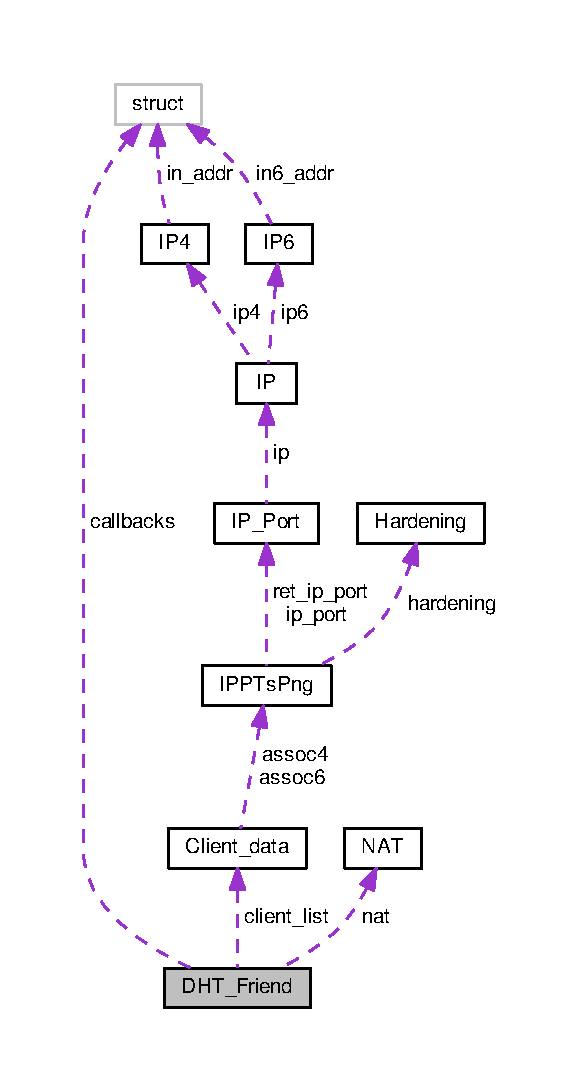
\includegraphics[width=279pt]{struct_d_h_t___friend__coll__graph}
\end{center}
\end{figure}
\subsection*{Data Fields}
\begin{DoxyCompactItemize}
\item 
\hypertarget{struct_d_h_t___friend_aaa806bb1136fb3d4b5d8d8970b596ff7}{uint8\+\_\+t {\bfseries public\+\_\+key} \mbox{[}crypto\+\_\+box\+\_\+\+P\+U\+B\+L\+I\+C\+K\+E\+Y\+B\+Y\+T\+E\+S\mbox{]}}\label{struct_d_h_t___friend_aaa806bb1136fb3d4b5d8d8970b596ff7}

\item 
\hypertarget{struct_d_h_t___friend_a49ef2b640a834a77b6e123355a4fea47}{\hyperlink{struct_client__data}{Client\+\_\+data} {\bfseries client\+\_\+list} \mbox{[}M\+A\+X\+\_\+\+F\+R\+I\+E\+N\+D\+\_\+\+C\+L\+I\+E\+N\+T\+S\mbox{]}}\label{struct_d_h_t___friend_a49ef2b640a834a77b6e123355a4fea47}

\item 
\hypertarget{struct_d_h_t___friend_acdb8d1d26f42ba99ca73f45cb5643d1e}{uint64\+\_\+t {\bfseries lastgetnode}}\label{struct_d_h_t___friend_acdb8d1d26f42ba99ca73f45cb5643d1e}

\item 
\hypertarget{struct_d_h_t___friend_aae62716bf77c5ba5fca784702d47a5ff}{uint32\+\_\+t {\bfseries bootstrap\+\_\+times}}\label{struct_d_h_t___friend_aae62716bf77c5ba5fca784702d47a5ff}

\item 
\hypertarget{struct_d_h_t___friend_a96318690475243d010825feb2a67b41c}{\hyperlink{struct_n_a_t}{N\+A\+T} {\bfseries nat}}\label{struct_d_h_t___friend_a96318690475243d010825feb2a67b41c}

\item 
\hypertarget{struct_d_h_t___friend_a712c4c639bfc0f5a8616eead3e24ca4e}{uint16\+\_\+t {\bfseries lock\+\_\+count}}\label{struct_d_h_t___friend_a712c4c639bfc0f5a8616eead3e24ca4e}

\item 
\hypertarget{struct_d_h_t___friend_a1ef2d93ffeb76ceb01d28ecb1244547c}{\begin{tabbing}
xx\=xx\=xx\=xx\=xx\=xx\=xx\=xx\=xx\=\kill
struct \{\\
\>void($\ast$ {\bfseries ip\_callback} )(void $\ast$, int32\_t, \hyperlink{struct_i_p___port}{IP\_Port})\\
\>void $\ast$ {\bfseries data}\\
\>int32\_t {\bfseries number}\\
\} {\bfseries callbacks} \mbox{[}DHT\_FRIEND\_MAX\_LOCKS\mbox{]}}\label{struct_d_h_t___friend_a1ef2d93ffeb76ceb01d28ecb1244547c}
\\

\end{tabbing}\end{DoxyCompactItemize}


\subsection{Detailed Description}


Definition at line 126 of file D\+H\+T.\+h.



The documentation for this struct was generated from the following file\+:\begin{DoxyCompactItemize}
\item 
toxcore/D\+H\+T.\+h\end{DoxyCompactItemize}

\hypertarget{struct_d_n_s___object}{\section{D\+N\+S\+\_\+\+Object Struct Reference}
\label{struct_d_n_s___object}\index{D\+N\+S\+\_\+\+Object@{D\+N\+S\+\_\+\+Object}}
}
\subsection*{Data Fields}
\begin{DoxyCompactItemize}
\item 
uint8\+\_\+t \hyperlink{struct_d_n_s___object_a46affbcc202b25e96fd1f5238e9e97e0}{temp\+\_\+pk} \mbox{[}crypto\+\_\+box\+\_\+\+P\+U\+B\+L\+I\+C\+K\+E\+Y\+B\+Y\+T\+E\+S\mbox{]}
\item 
uint8\+\_\+t \hyperlink{struct_d_n_s___object_a3652189f09ee098ced277788337d95e7}{temp\+\_\+sk} \mbox{[}crypto\+\_\+box\+\_\+\+S\+E\+C\+R\+E\+T\+K\+E\+Y\+B\+Y\+T\+E\+S\mbox{]}
\item 
uint8\+\_\+t \hyperlink{struct_d_n_s___object_acc2e1517636c724d8778c873a4fce5e1}{server\+\_\+public\+\_\+key} \mbox{[}crypto\+\_\+box\+\_\+\+P\+U\+B\+L\+I\+C\+K\+E\+Y\+B\+Y\+T\+E\+S\mbox{]}
\item 
uint8\+\_\+t \hyperlink{struct_d_n_s___object_a0f4a120c7bd84eb7beebe6c163ce5744}{shared\+\_\+key} \mbox{[}\hyperlink{crypto__core_8h_aade7cd33abc5668970c55ed009ab00c8}{crypto\+\_\+box\+\_\+\+K\+E\+Y\+B\+Y\+T\+E\+S}\mbox{]}
\item 
uint32\+\_\+t \hyperlink{struct_d_n_s___object_aa2f9785a9d9116cc4592db06375cb887}{nonce}
\item 
uint32\+\_\+t \hyperlink{struct_d_n_s___object_a9bf0718fc917292d63aa2667d22c0502}{nonce\+\_\+start}
\end{DoxyCompactItemize}


\subsection{Detailed Description}


Definition at line 48 of file toxdns.\+c.



\subsection{Field Documentation}
\hypertarget{struct_d_n_s___object_aa2f9785a9d9116cc4592db06375cb887}{\index{D\+N\+S\+\_\+\+Object@{D\+N\+S\+\_\+\+Object}!nonce@{nonce}}
\index{nonce@{nonce}!D\+N\+S\+\_\+\+Object@{D\+N\+S\+\_\+\+Object}}
\subsubsection[{nonce}]{\setlength{\rightskip}{0pt plus 5cm}uint32\+\_\+t nonce}}\label{struct_d_n_s___object_aa2f9785a9d9116cc4592db06375cb887}


Definition at line 53 of file toxdns.\+c.



Referenced by dns\+\_\+new\+\_\+temp\+\_\+keys(), and tox\+\_\+generate\+\_\+dns3\+\_\+string().

\hypertarget{struct_d_n_s___object_a9bf0718fc917292d63aa2667d22c0502}{\index{D\+N\+S\+\_\+\+Object@{D\+N\+S\+\_\+\+Object}!nonce\+\_\+start@{nonce\+\_\+start}}
\index{nonce\+\_\+start@{nonce\+\_\+start}!D\+N\+S\+\_\+\+Object@{D\+N\+S\+\_\+\+Object}}
\subsubsection[{nonce\+\_\+start}]{\setlength{\rightskip}{0pt plus 5cm}uint32\+\_\+t nonce\+\_\+start}}\label{struct_d_n_s___object_a9bf0718fc917292d63aa2667d22c0502}


Definition at line 54 of file toxdns.\+c.



Referenced by dns\+\_\+new\+\_\+temp\+\_\+keys(), and tox\+\_\+generate\+\_\+dns3\+\_\+string().

\hypertarget{struct_d_n_s___object_acc2e1517636c724d8778c873a4fce5e1}{\index{D\+N\+S\+\_\+\+Object@{D\+N\+S\+\_\+\+Object}!server\+\_\+public\+\_\+key@{server\+\_\+public\+\_\+key}}
\index{server\+\_\+public\+\_\+key@{server\+\_\+public\+\_\+key}!D\+N\+S\+\_\+\+Object@{D\+N\+S\+\_\+\+Object}}
\subsubsection[{server\+\_\+public\+\_\+key}]{\setlength{\rightskip}{0pt plus 5cm}uint8\+\_\+t server\+\_\+public\+\_\+key\mbox{[}crypto\+\_\+box\+\_\+\+P\+U\+B\+L\+I\+C\+K\+E\+Y\+B\+Y\+T\+E\+S\mbox{]}}}\label{struct_d_n_s___object_acc2e1517636c724d8778c873a4fce5e1}


Definition at line 51 of file toxdns.\+c.



Referenced by dns\+\_\+new\+\_\+temp\+\_\+keys(), and tox\+\_\+dns3\+\_\+new().

\hypertarget{struct_d_n_s___object_a0f4a120c7bd84eb7beebe6c163ce5744}{\index{D\+N\+S\+\_\+\+Object@{D\+N\+S\+\_\+\+Object}!shared\+\_\+key@{shared\+\_\+key}}
\index{shared\+\_\+key@{shared\+\_\+key}!D\+N\+S\+\_\+\+Object@{D\+N\+S\+\_\+\+Object}}
\subsubsection[{shared\+\_\+key}]{\setlength{\rightskip}{0pt plus 5cm}uint8\+\_\+t shared\+\_\+key\mbox{[}{\bf crypto\+\_\+box\+\_\+\+K\+E\+Y\+B\+Y\+T\+E\+S}\mbox{]}}}\label{struct_d_n_s___object_a0f4a120c7bd84eb7beebe6c163ce5744}


Definition at line 52 of file toxdns.\+c.



Referenced by dns\+\_\+new\+\_\+temp\+\_\+keys(), tox\+\_\+decrypt\+\_\+dns3\+\_\+\+T\+X\+T(), and tox\+\_\+generate\+\_\+dns3\+\_\+string().

\hypertarget{struct_d_n_s___object_a46affbcc202b25e96fd1f5238e9e97e0}{\index{D\+N\+S\+\_\+\+Object@{D\+N\+S\+\_\+\+Object}!temp\+\_\+pk@{temp\+\_\+pk}}
\index{temp\+\_\+pk@{temp\+\_\+pk}!D\+N\+S\+\_\+\+Object@{D\+N\+S\+\_\+\+Object}}
\subsubsection[{temp\+\_\+pk}]{\setlength{\rightskip}{0pt plus 5cm}uint8\+\_\+t temp\+\_\+pk\mbox{[}crypto\+\_\+box\+\_\+\+P\+U\+B\+L\+I\+C\+K\+E\+Y\+B\+Y\+T\+E\+S\mbox{]}}}\label{struct_d_n_s___object_a46affbcc202b25e96fd1f5238e9e97e0}


Definition at line 49 of file toxdns.\+c.



Referenced by dns\+\_\+new\+\_\+temp\+\_\+keys(), and tox\+\_\+generate\+\_\+dns3\+\_\+string().

\hypertarget{struct_d_n_s___object_a3652189f09ee098ced277788337d95e7}{\index{D\+N\+S\+\_\+\+Object@{D\+N\+S\+\_\+\+Object}!temp\+\_\+sk@{temp\+\_\+sk}}
\index{temp\+\_\+sk@{temp\+\_\+sk}!D\+N\+S\+\_\+\+Object@{D\+N\+S\+\_\+\+Object}}
\subsubsection[{temp\+\_\+sk}]{\setlength{\rightskip}{0pt plus 5cm}uint8\+\_\+t temp\+\_\+sk\mbox{[}crypto\+\_\+box\+\_\+\+S\+E\+C\+R\+E\+T\+K\+E\+Y\+B\+Y\+T\+E\+S\mbox{]}}}\label{struct_d_n_s___object_a3652189f09ee098ced277788337d95e7}


Definition at line 50 of file toxdns.\+c.



Referenced by dns\+\_\+new\+\_\+temp\+\_\+keys().



The documentation for this struct was generated from the following file\+:\begin{DoxyCompactItemize}
\item 
toxdns/\hyperlink{toxdns_8c}{toxdns.\+c}\end{DoxyCompactItemize}

\hypertarget{struct_file___sender}{\section{File\+\_\+\+Sender Struct Reference}
\label{struct_file___sender}\index{File\+\_\+\+Sender@{File\+\_\+\+Sender}}
}
\subsection*{Data Fields}
\begin{DoxyCompactItemize}
\item 
F\+I\+L\+E $\ast$ \hyperlink{struct_file___sender_a702945180aa732857b380a007a7e2a21}{file}
\item 
uint32\+\_\+t \hyperlink{struct_file___sender_af02b3246ba69ea99fddd081f6e95598f}{friendnum}
\item 
uint32\+\_\+t \hyperlink{struct_file___sender_a32e4dffe2d73a1eeddb1bc8ce5511367}{filenumber}
\end{DoxyCompactItemize}


\subsection{Detailed Description}


Definition at line 116 of file n\+Tox.\+c.



\subsection{Field Documentation}
\hypertarget{struct_file___sender_a702945180aa732857b380a007a7e2a21}{\index{File\+\_\+\+Sender@{File\+\_\+\+Sender}!file@{file}}
\index{file@{file}!File\+\_\+\+Sender@{File\+\_\+\+Sender}}
\subsubsection[{file}]{\setlength{\rightskip}{0pt plus 5cm}F\+I\+L\+E$\ast$ file}}\label{struct_file___sender_a702945180aa732857b380a007a7e2a21}


Definition at line 117 of file n\+Tox.\+c.



Referenced by add\+\_\+filesender(), file\+\_\+print\+\_\+control(), print\+\_\+online(), and tox\+\_\+file\+\_\+chunk\+\_\+request().

\hypertarget{struct_file___sender_a32e4dffe2d73a1eeddb1bc8ce5511367}{\index{File\+\_\+\+Sender@{File\+\_\+\+Sender}!filenumber@{filenumber}}
\index{filenumber@{filenumber}!File\+\_\+\+Sender@{File\+\_\+\+Sender}}
\subsubsection[{filenumber}]{\setlength{\rightskip}{0pt plus 5cm}uint32\+\_\+t filenumber}}\label{struct_file___sender_a32e4dffe2d73a1eeddb1bc8ce5511367}


Definition at line 119 of file n\+Tox.\+c.



Referenced by add\+\_\+filesender().

\hypertarget{struct_file___sender_af02b3246ba69ea99fddd081f6e95598f}{\index{File\+\_\+\+Sender@{File\+\_\+\+Sender}!friendnum@{friendnum}}
\index{friendnum@{friendnum}!File\+\_\+\+Sender@{File\+\_\+\+Sender}}
\subsubsection[{friendnum}]{\setlength{\rightskip}{0pt plus 5cm}uint32\+\_\+t friendnum}}\label{struct_file___sender_af02b3246ba69ea99fddd081f6e95598f}


Definition at line 118 of file n\+Tox.\+c.



Referenced by add\+\_\+filesender().



The documentation for this struct was generated from the following file\+:\begin{DoxyCompactItemize}
\item 
testing/\hyperlink{n_tox_8c}{n\+Tox.\+c}\end{DoxyCompactItemize}

\hypertarget{struct_file__t}{\section{File\+\_\+t Struct Reference}
\label{struct_file__t}\index{File\+\_\+t@{File\+\_\+t}}
}
\subsection*{Data Fields}
\begin{DoxyCompactItemize}
\item 
\hypertarget{struct_file__t_a702945180aa732857b380a007a7e2a21}{F\+I\+L\+E $\ast$ {\bfseries file}}\label{struct_file__t_a702945180aa732857b380a007a7e2a21}

\item 
\hypertarget{struct_file__t_af02b3246ba69ea99fddd081f6e95598f}{uint32\+\_\+t {\bfseries friendnum}}\label{struct_file__t_af02b3246ba69ea99fddd081f6e95598f}

\item 
\hypertarget{struct_file__t_a32e4dffe2d73a1eeddb1bc8ce5511367}{uint32\+\_\+t {\bfseries filenumber}}\label{struct_file__t_a32e4dffe2d73a1eeddb1bc8ce5511367}

\end{DoxyCompactItemize}


\subsection{Detailed Description}


Definition at line 47 of file tox\+\_\+sync.\+c.



The documentation for this struct was generated from the following file\+:\begin{DoxyCompactItemize}
\item 
testing/tox\+\_\+sync.\+c\end{DoxyCompactItemize}

\hypertarget{struct_file___transfers}{\section{File\+\_\+\+Transfers Struct Reference}
\label{struct_file___transfers}\index{File\+\_\+\+Transfers@{File\+\_\+\+Transfers}}
}


{\ttfamily \#include $<$Messenger.\+h$>$}

\subsection*{Data Fields}
\begin{DoxyCompactItemize}
\item 
uint64\+\_\+t \hyperlink{struct_file___transfers_af931a8871310b4dad23f0f0b0f623560}{size}
\item 
uint64\+\_\+t \hyperlink{struct_file___transfers_ae0a9ddd27f7c6669cb964f6245b2550d}{transferred}
\item 
uint8\+\_\+t \hyperlink{struct_file___transfers_ade818037fd6c985038ff29656089758d}{status}
\item 
uint8\+\_\+t \hyperlink{struct_file___transfers_a84bd3ab7c2cbad7fb0b6233504515973}{paused}
\item 
uint32\+\_\+t \hyperlink{struct_file___transfers_a14f807289cc5523a0081c7f87aed647e}{last\+\_\+packet\+\_\+number}
\item 
uint64\+\_\+t \hyperlink{struct_file___transfers_a23cc26eca74ddec84f975c0be5496457}{requested}
\item 
unsigned int \hyperlink{struct_file___transfers_ae5c1661a0e1ed999ed054d837989556b}{slots\+\_\+allocated}
\item 
uint8\+\_\+t \hyperlink{struct_file___transfers_aa32dbb3439461c6ccc1a52ff15bcb22e}{id} \mbox{[}\hyperlink{_messenger_8h_a2f1a1efe7944eb3e268659d28b5db7d3}{F\+I\+L\+E\+\_\+\+I\+D\+\_\+\+L\+E\+N\+G\+T\+H}\mbox{]}
\end{DoxyCompactItemize}


\subsection{Detailed Description}


Definition at line 130 of file Messenger.\+h.



\subsection{Field Documentation}
\hypertarget{struct_file___transfers_aa32dbb3439461c6ccc1a52ff15bcb22e}{\index{File\+\_\+\+Transfers@{File\+\_\+\+Transfers}!id@{id}}
\index{id@{id}!File\+\_\+\+Transfers@{File\+\_\+\+Transfers}}
\subsubsection[{id}]{\setlength{\rightskip}{0pt plus 5cm}uint8\+\_\+t id\mbox{[}{\bf F\+I\+L\+E\+\_\+\+I\+D\+\_\+\+L\+E\+N\+G\+T\+H}\mbox{]}}}\label{struct_file___transfers_aa32dbb3439461c6ccc1a52ff15bcb22e}


Definition at line 138 of file Messenger.\+h.



Referenced by file\+\_\+get\+\_\+id(), handle\+\_\+packet(), and new\+\_\+filesender().

\hypertarget{struct_file___transfers_a14f807289cc5523a0081c7f87aed647e}{\index{File\+\_\+\+Transfers@{File\+\_\+\+Transfers}!last\+\_\+packet\+\_\+number@{last\+\_\+packet\+\_\+number}}
\index{last\+\_\+packet\+\_\+number@{last\+\_\+packet\+\_\+number}!File\+\_\+\+Transfers@{File\+\_\+\+Transfers}}
\subsubsection[{last\+\_\+packet\+\_\+number}]{\setlength{\rightskip}{0pt plus 5cm}uint32\+\_\+t last\+\_\+packet\+\_\+number}}\label{struct_file___transfers_a14f807289cc5523a0081c7f87aed647e}


Definition at line 135 of file Messenger.\+h.



Referenced by do\+\_\+reqchunk\+\_\+filecb(), and file\+\_\+data().

\hypertarget{struct_file___transfers_a84bd3ab7c2cbad7fb0b6233504515973}{\index{File\+\_\+\+Transfers@{File\+\_\+\+Transfers}!paused@{paused}}
\index{paused@{paused}!File\+\_\+\+Transfers@{File\+\_\+\+Transfers}}
\subsubsection[{paused}]{\setlength{\rightskip}{0pt plus 5cm}uint8\+\_\+t paused}}\label{struct_file___transfers_a84bd3ab7c2cbad7fb0b6233504515973}


Definition at line 134 of file Messenger.\+h.



Referenced by do\+\_\+reqchunk\+\_\+filecb(), file\+\_\+control(), handle\+\_\+filecontrol(), handle\+\_\+packet(), and new\+\_\+filesender().

\hypertarget{struct_file___transfers_a23cc26eca74ddec84f975c0be5496457}{\index{File\+\_\+\+Transfers@{File\+\_\+\+Transfers}!requested@{requested}}
\index{requested@{requested}!File\+\_\+\+Transfers@{File\+\_\+\+Transfers}}
\subsubsection[{requested}]{\setlength{\rightskip}{0pt plus 5cm}uint64\+\_\+t requested}}\label{struct_file___transfers_a23cc26eca74ddec84f975c0be5496457}


Definition at line 136 of file Messenger.\+h.



Referenced by do\+\_\+reqchunk\+\_\+filecb(), file\+\_\+data(), handle\+\_\+filecontrol(), and new\+\_\+filesender().

\hypertarget{struct_file___transfers_af931a8871310b4dad23f0f0b0f623560}{\index{File\+\_\+\+Transfers@{File\+\_\+\+Transfers}!size@{size}}
\index{size@{size}!File\+\_\+\+Transfers@{File\+\_\+\+Transfers}}
\subsubsection[{size}]{\setlength{\rightskip}{0pt plus 5cm}uint64\+\_\+t size}}\label{struct_file___transfers_af931a8871310b4dad23f0f0b0f623560}


Definition at line 131 of file Messenger.\+h.



Referenced by do\+\_\+reqchunk\+\_\+filecb(), file\+\_\+data(), file\+\_\+dataremaining(), file\+\_\+seek(), handle\+\_\+filecontrol(), handle\+\_\+packet(), and new\+\_\+filesender().

\hypertarget{struct_file___transfers_ae5c1661a0e1ed999ed054d837989556b}{\index{File\+\_\+\+Transfers@{File\+\_\+\+Transfers}!slots\+\_\+allocated@{slots\+\_\+allocated}}
\index{slots\+\_\+allocated@{slots\+\_\+allocated}!File\+\_\+\+Transfers@{File\+\_\+\+Transfers}}
\subsubsection[{slots\+\_\+allocated}]{\setlength{\rightskip}{0pt plus 5cm}unsigned int slots\+\_\+allocated}}\label{struct_file___transfers_ae5c1661a0e1ed999ed054d837989556b}


Definition at line 137 of file Messenger.\+h.



Referenced by do\+\_\+reqchunk\+\_\+filecb(), file\+\_\+data(), and new\+\_\+filesender().

\hypertarget{struct_file___transfers_ade818037fd6c985038ff29656089758d}{\index{File\+\_\+\+Transfers@{File\+\_\+\+Transfers}!status@{status}}
\index{status@{status}!File\+\_\+\+Transfers@{File\+\_\+\+Transfers}}
\subsubsection[{status}]{\setlength{\rightskip}{0pt plus 5cm}uint8\+\_\+t status}}\label{struct_file___transfers_ade818037fd6c985038ff29656089758d}


Definition at line 133 of file Messenger.\+h.



Referenced by break\+\_\+files(), do\+\_\+reqchunk\+\_\+filecb(), file\+\_\+control(), file\+\_\+data(), file\+\_\+dataremaining(), file\+\_\+get\+\_\+id(), file\+\_\+seek(), handle\+\_\+filecontrol(), handle\+\_\+packet(), and new\+\_\+filesender().

\hypertarget{struct_file___transfers_ae0a9ddd27f7c6669cb964f6245b2550d}{\index{File\+\_\+\+Transfers@{File\+\_\+\+Transfers}!transferred@{transferred}}
\index{transferred@{transferred}!File\+\_\+\+Transfers@{File\+\_\+\+Transfers}}
\subsubsection[{transferred}]{\setlength{\rightskip}{0pt plus 5cm}uint64\+\_\+t transferred}}\label{struct_file___transfers_ae0a9ddd27f7c6669cb964f6245b2550d}


Definition at line 132 of file Messenger.\+h.



Referenced by do\+\_\+reqchunk\+\_\+filecb(), file\+\_\+data(), file\+\_\+dataremaining(), file\+\_\+seek(), handle\+\_\+filecontrol(), handle\+\_\+packet(), and new\+\_\+filesender().



The documentation for this struct was generated from the following file\+:\begin{DoxyCompactItemize}
\item 
toxcore/\hyperlink{_messenger_8h}{Messenger.\+h}\end{DoxyCompactItemize}

\hypertarget{struct_friend}{\section{Friend Struct Reference}
\label{struct_friend}\index{Friend@{Friend}}
}


{\ttfamily \#include $<$Messenger.\+h$>$}



Collaboration diagram for Friend\+:
\nopagebreak
\begin{figure}[H]
\begin{center}
\leavevmode
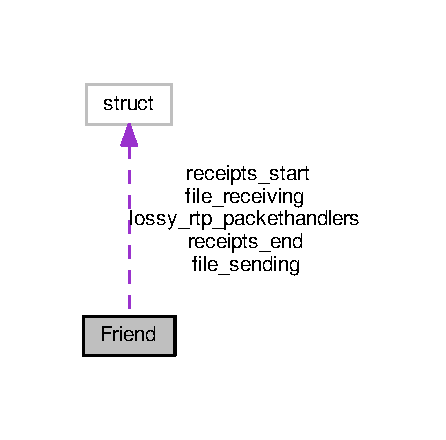
\includegraphics[width=214pt]{db/d78/struct_friend__coll__graph}
\end{center}
\end{figure}
\subsection*{Data Fields}
\begin{DoxyCompactItemize}
\item 
uint8\+\_\+t \hyperlink{struct_friend_ab42b4c90d81ac99b968c3edd1e21d706}{real\+\_\+pk} \mbox{[}crypto\+\_\+box\+\_\+\+P\+U\+B\+L\+I\+C\+K\+E\+Y\+B\+Y\+T\+E\+S\mbox{]}
\item 
int \hyperlink{struct_friend_aed1c0bb5aeba492059252d0084c8ae9b}{friendcon\+\_\+id}
\item 
uint64\+\_\+t \hyperlink{struct_friend_a1cea2470caaf4282313efe944e95bf35}{friendrequest\+\_\+lastsent}
\item 
uint32\+\_\+t \hyperlink{struct_friend_a671d1f4ab926cb9dc297c3f2743560d4}{friendrequest\+\_\+timeout}
\item 
uint8\+\_\+t \hyperlink{struct_friend_ade818037fd6c985038ff29656089758d}{status}
\item 
uint8\+\_\+t \hyperlink{struct_friend_ae1a1264e17ce4eedae67c283a09236e6}{info} \mbox{[}\hyperlink{friend__requests_8h_a89b7e8b76560d3513fd3b054de738553}{M\+A\+X\+\_\+\+F\+R\+I\+E\+N\+D\+\_\+\+R\+E\+Q\+U\+E\+S\+T\+\_\+\+D\+A\+T\+A\+\_\+\+S\+I\+Z\+E}\mbox{]}
\item 
uint8\+\_\+t \hyperlink{struct_friend_a11b8cc6595eea79e65c978209278e683}{name} \mbox{[}\hyperlink{_messenger_8h_a0c397a708cec89c74029582574516b30}{M\+A\+X\+\_\+\+N\+A\+M\+E\+\_\+\+L\+E\+N\+G\+T\+H}\mbox{]}
\item 
uint16\+\_\+t \hyperlink{struct_friend_a3573d7a906b26e9999cd74f2c4066601}{name\+\_\+length}
\item 
uint8\+\_\+t \hyperlink{struct_friend_acc966be04e3e27e15dfd493c3e9cff89}{name\+\_\+sent}
\item 
uint8\+\_\+t \hyperlink{struct_friend_a8f12612ac1191135a1a5b1cbcbc82852}{statusmessage} \mbox{[}\hyperlink{_messenger_8h_a0d1a4b91dd43b4cb07dfefab7fc6bee1}{M\+A\+X\+\_\+\+S\+T\+A\+T\+U\+S\+M\+E\+S\+S\+A\+G\+E\+\_\+\+L\+E\+N\+G\+T\+H}\mbox{]}
\item 
uint16\+\_\+t \hyperlink{struct_friend_a43fe9dde52dc12e90933150eca91c0c3}{statusmessage\+\_\+length}
\item 
uint8\+\_\+t \hyperlink{struct_friend_ad39189cd22b356c314e4d980b55db259}{statusmessage\+\_\+sent}
\item 
\hyperlink{_messenger_8h_aa55a7166581c83a07f49f9392447986c}{U\+S\+E\+R\+S\+T\+A\+T\+U\+S} \hyperlink{struct_friend_adde524f5a15465585cbc2543cd0b2710}{userstatus}
\item 
uint8\+\_\+t \hyperlink{struct_friend_af7c74fd36acb972c3a8641fb0781e37e}{userstatus\+\_\+sent}
\item 
uint8\+\_\+t \hyperlink{struct_friend_a68e945edd5a63c22371edf481c788d88}{user\+\_\+istyping}
\item 
uint8\+\_\+t \hyperlink{struct_friend_a8d9e9aef86444e0cde8ec0314f60907e}{user\+\_\+istyping\+\_\+sent}
\item 
uint8\+\_\+t \hyperlink{struct_friend_a4eb96aff01799d54246cc48854a47175}{is\+\_\+typing}
\item 
uint16\+\_\+t \hyperlink{struct_friend_ac0ae002db55ef8f8366de10ec005b65a}{info\+\_\+size}
\item 
uint32\+\_\+t \hyperlink{struct_friend_aa4420a99dd00b4884b23150e4226b2ea}{message\+\_\+id}
\item 
uint32\+\_\+t \hyperlink{struct_friend_a0fae9801a4789a368f90125119e31f3f}{friendrequest\+\_\+nospam}
\item 
uint64\+\_\+t \hyperlink{struct_friend_a8f99c48eb6b3ea472806495135ab6792}{last\+\_\+seen\+\_\+time}
\item 
uint8\+\_\+t \hyperlink{struct_friend_ac213b32e59c2e4a64923c453b100c4e4}{last\+\_\+connection\+\_\+udp\+\_\+tcp}
\item 
struct \hyperlink{struct_file___transfers}{File\+\_\+\+Transfers} \hyperlink{struct_friend_a51d0849a59878ad9e4b67123a1c87037}{file\+\_\+sending} \mbox{[}\hyperlink{_messenger_8h_a5e5c08c689138cd56d6c1a16d3eea793}{M\+A\+X\+\_\+\+C\+O\+N\+C\+U\+R\+R\+E\+N\+T\+\_\+\+F\+I\+L\+E\+\_\+\+P\+I\+P\+E\+S}\mbox{]}
\item 
unsigned int \hyperlink{struct_friend_ac4dcaccdfc6f354a321622e84b27b856}{num\+\_\+sending\+\_\+files}
\item 
struct \hyperlink{struct_file___transfers}{File\+\_\+\+Transfers} \hyperlink{struct_friend_ab14e1c3452717012d0bbb0dad068e9f6}{file\+\_\+receiving} \mbox{[}\hyperlink{_messenger_8h_a5e5c08c689138cd56d6c1a16d3eea793}{M\+A\+X\+\_\+\+C\+O\+N\+C\+U\+R\+R\+E\+N\+T\+\_\+\+F\+I\+L\+E\+\_\+\+P\+I\+P\+E\+S}\mbox{]}
\item 
\begin{tabbing}
xx\=xx\=xx\=xx\=xx\=xx\=xx\=xx\=xx\=\kill
struct \{\\
\>int($\ast$ \hyperlink{struct_friend_a726a4dcb820b33fd434494d56f532867}{function} )(\hyperlink{struct_messenger}{Messenger} $\ast$\hyperlink{_messenger__test_8c_aea6eb6c7c30a659f1b0dee83eaf03ea2}{m}, uint32\_t \\
\>\>friendnumber, const uint8\_t \\
\>\>$\ast$data, uint16\_t len, void \\
\>\>$\ast$\hyperlink{struct_friend_a077376d12464f945e2414d5499c79b3f}{object})\\
\>void $\ast$ \hyperlink{struct_friend_a077376d12464f945e2414d5499c79b3f}{object}\\
\} \hyperlink{struct_friend_af8c513c69f17fc044615b18ec03f9911}{lossy\_rtp\_packethandlers} \mbox{[}\hyperlink{_messenger_8h_a9e9b181fad5abaed171e4b4481490d1e}{PACKET\_LOSSY\_AV\_RESERVED}\mbox{]}\\

\end{tabbing}\item 
struct \hyperlink{struct_receipts}{Receipts} $\ast$ \hyperlink{struct_friend_a49fea7d214384bfdb887ce868fef0e93}{receipts\+\_\+start}
\item 
struct \hyperlink{struct_receipts}{Receipts} $\ast$ \hyperlink{struct_friend_ad4ff64ea096ee2af6b53f8d9f7901776}{receipts\+\_\+end}
\end{DoxyCompactItemize}


\subsection{Detailed Description}


Definition at line 173 of file Messenger.\+h.



\subsection{Field Documentation}
\hypertarget{struct_friend_ab14e1c3452717012d0bbb0dad068e9f6}{\index{Friend@{Friend}!file\+\_\+receiving@{file\+\_\+receiving}}
\index{file\+\_\+receiving@{file\+\_\+receiving}!Friend@{Friend}}
\subsubsection[{file\+\_\+receiving}]{\setlength{\rightskip}{0pt plus 5cm}struct {\bf File\+\_\+\+Transfers} file\+\_\+receiving\mbox{[}{\bf M\+A\+X\+\_\+\+C\+O\+N\+C\+U\+R\+R\+E\+N\+T\+\_\+\+F\+I\+L\+E\+\_\+\+P\+I\+P\+E\+S}\mbox{]}}}\label{struct_friend_ab14e1c3452717012d0bbb0dad068e9f6}


Definition at line 199 of file Messenger.\+h.



Referenced by break\+\_\+files(), file\+\_\+control(), file\+\_\+dataremaining(), file\+\_\+get\+\_\+id(), file\+\_\+seek(), handle\+\_\+filecontrol(), and handle\+\_\+packet().

\hypertarget{struct_friend_a51d0849a59878ad9e4b67123a1c87037}{\index{Friend@{Friend}!file\+\_\+sending@{file\+\_\+sending}}
\index{file\+\_\+sending@{file\+\_\+sending}!Friend@{Friend}}
\subsubsection[{file\+\_\+sending}]{\setlength{\rightskip}{0pt plus 5cm}struct {\bf File\+\_\+\+Transfers} file\+\_\+sending\mbox{[}{\bf M\+A\+X\+\_\+\+C\+O\+N\+C\+U\+R\+R\+E\+N\+T\+\_\+\+F\+I\+L\+E\+\_\+\+P\+I\+P\+E\+S}\mbox{]}}}\label{struct_friend_a51d0849a59878ad9e4b67123a1c87037}


Definition at line 197 of file Messenger.\+h.



Referenced by break\+\_\+files(), do\+\_\+reqchunk\+\_\+filecb(), file\+\_\+control(), file\+\_\+data(), file\+\_\+dataremaining(), file\+\_\+get\+\_\+id(), file\+\_\+seek(), handle\+\_\+filecontrol(), and new\+\_\+filesender().

\hypertarget{struct_friend_aed1c0bb5aeba492059252d0084c8ae9b}{\index{Friend@{Friend}!friendcon\+\_\+id@{friendcon\+\_\+id}}
\index{friendcon\+\_\+id@{friendcon\+\_\+id}!Friend@{Friend}}
\subsubsection[{friendcon\+\_\+id}]{\setlength{\rightskip}{0pt plus 5cm}int friendcon\+\_\+id}}\label{struct_friend_aed1c0bb5aeba492059252d0084c8ae9b}


Definition at line 175 of file Messenger.\+h.



Referenced by do\+\_\+friends(), do\+\_\+reqchunk\+\_\+filecb(), file\+\_\+data(), friend\+\_\+received\+\_\+packet(), getfriendcon\+\_\+id(), init\+\_\+new\+\_\+friend(), m\+\_\+delfriend(), m\+\_\+get\+\_\+friend\+\_\+connectionstatus(), m\+\_\+send\+\_\+message\+\_\+generic(), send\+\_\+custom\+\_\+lossless\+\_\+packet(), send\+\_\+custom\+\_\+lossy\+\_\+packet(), send\+\_\+file\+\_\+data\+\_\+packet(), send\+\_\+online\+\_\+packet(), and write\+\_\+cryptpacket\+\_\+id().

\hypertarget{struct_friend_a1cea2470caaf4282313efe944e95bf35}{\index{Friend@{Friend}!friendrequest\+\_\+lastsent@{friendrequest\+\_\+lastsent}}
\index{friendrequest\+\_\+lastsent@{friendrequest\+\_\+lastsent}!Friend@{Friend}}
\subsubsection[{friendrequest\+\_\+lastsent}]{\setlength{\rightskip}{0pt plus 5cm}uint64\+\_\+t friendrequest\+\_\+lastsent}}\label{struct_friend_a1cea2470caaf4282313efe944e95bf35}


Definition at line 177 of file Messenger.\+h.



Referenced by check\+\_\+friend\+\_\+request\+\_\+timed\+\_\+out(), do\+\_\+friends(), and init\+\_\+new\+\_\+friend().

\hypertarget{struct_friend_a0fae9801a4789a368f90125119e31f3f}{\index{Friend@{Friend}!friendrequest\+\_\+nospam@{friendrequest\+\_\+nospam}}
\index{friendrequest\+\_\+nospam@{friendrequest\+\_\+nospam}!Friend@{Friend}}
\subsubsection[{friendrequest\+\_\+nospam}]{\setlength{\rightskip}{0pt plus 5cm}uint32\+\_\+t friendrequest\+\_\+nospam}}\label{struct_friend_a0fae9801a4789a368f90125119e31f3f}


Definition at line 194 of file Messenger.\+h.



Referenced by do\+\_\+friends(), friends\+\_\+list\+\_\+save(), and m\+\_\+addfriend().

\hypertarget{struct_friend_a671d1f4ab926cb9dc297c3f2743560d4}{\index{Friend@{Friend}!friendrequest\+\_\+timeout@{friendrequest\+\_\+timeout}}
\index{friendrequest\+\_\+timeout@{friendrequest\+\_\+timeout}!Friend@{Friend}}
\subsubsection[{friendrequest\+\_\+timeout}]{\setlength{\rightskip}{0pt plus 5cm}uint32\+\_\+t friendrequest\+\_\+timeout}}\label{struct_friend_a671d1f4ab926cb9dc297c3f2743560d4}


Definition at line 178 of file Messenger.\+h.



Referenced by check\+\_\+friend\+\_\+request\+\_\+timed\+\_\+out(), and m\+\_\+addfriend().

\hypertarget{struct_friend_a726a4dcb820b33fd434494d56f532867}{\index{Friend@{Friend}!function@{function}}
\index{function@{function}!Friend@{Friend}}
\subsubsection[{function}]{\setlength{\rightskip}{0pt plus 5cm}int($\ast$ function)({\bf Messenger} $\ast${\bf m}, uint32\+\_\+t friendnumber, const uint8\+\_\+t $\ast$data, uint16\+\_\+t len, void $\ast${\bf object})}}\label{struct_friend_a726a4dcb820b33fd434494d56f532867}


Definition at line 202 of file Messenger.\+h.



Referenced by handle\+\_\+custom\+\_\+lossy\+\_\+packet(), and m\+\_\+callback\+\_\+rtp\+\_\+packet().

\hypertarget{struct_friend_ae1a1264e17ce4eedae67c283a09236e6}{\index{Friend@{Friend}!info@{info}}
\index{info@{info}!Friend@{Friend}}
\subsubsection[{info}]{\setlength{\rightskip}{0pt plus 5cm}uint8\+\_\+t info\mbox{[}{\bf M\+A\+X\+\_\+\+F\+R\+I\+E\+N\+D\+\_\+\+R\+E\+Q\+U\+E\+S\+T\+\_\+\+D\+A\+T\+A\+\_\+\+S\+I\+Z\+E}\mbox{]}}}\label{struct_friend_ae1a1264e17ce4eedae67c283a09236e6}


Definition at line 180 of file Messenger.\+h.



Referenced by do\+\_\+friends(), friends\+\_\+list\+\_\+save(), and m\+\_\+addfriend().

\hypertarget{struct_friend_ac0ae002db55ef8f8366de10ec005b65a}{\index{Friend@{Friend}!info\+\_\+size@{info\+\_\+size}}
\index{info\+\_\+size@{info\+\_\+size}!Friend@{Friend}}
\subsubsection[{info\+\_\+size}]{\setlength{\rightskip}{0pt plus 5cm}uint16\+\_\+t info\+\_\+size}}\label{struct_friend_ac0ae002db55ef8f8366de10ec005b65a}


Definition at line 192 of file Messenger.\+h.



Referenced by do\+\_\+friends(), friends\+\_\+list\+\_\+save(), and m\+\_\+addfriend().

\hypertarget{struct_friend_a4eb96aff01799d54246cc48854a47175}{\index{Friend@{Friend}!is\+\_\+typing@{is\+\_\+typing}}
\index{is\+\_\+typing@{is\+\_\+typing}!Friend@{Friend}}
\subsubsection[{is\+\_\+typing}]{\setlength{\rightskip}{0pt plus 5cm}uint8\+\_\+t is\+\_\+typing}}\label{struct_friend_a4eb96aff01799d54246cc48854a47175}


Definition at line 191 of file Messenger.\+h.



Referenced by init\+\_\+new\+\_\+friend(), m\+\_\+get\+\_\+istyping(), and set\+\_\+friend\+\_\+typing().

\hypertarget{struct_friend_ac213b32e59c2e4a64923c453b100c4e4}{\index{Friend@{Friend}!last\+\_\+connection\+\_\+udp\+\_\+tcp@{last\+\_\+connection\+\_\+udp\+\_\+tcp}}
\index{last\+\_\+connection\+\_\+udp\+\_\+tcp@{last\+\_\+connection\+\_\+udp\+\_\+tcp}!Friend@{Friend}}
\subsubsection[{last\+\_\+connection\+\_\+udp\+\_\+tcp}]{\setlength{\rightskip}{0pt plus 5cm}uint8\+\_\+t last\+\_\+connection\+\_\+udp\+\_\+tcp}}\label{struct_friend_ac213b32e59c2e4a64923c453b100c4e4}


Definition at line 196 of file Messenger.\+h.



Referenced by check\+\_\+friend\+\_\+tcp\+\_\+udp().

\hypertarget{struct_friend_a8f99c48eb6b3ea472806495135ab6792}{\index{Friend@{Friend}!last\+\_\+seen\+\_\+time@{last\+\_\+seen\+\_\+time}}
\index{last\+\_\+seen\+\_\+time@{last\+\_\+seen\+\_\+time}!Friend@{Friend}}
\subsubsection[{last\+\_\+seen\+\_\+time}]{\setlength{\rightskip}{0pt plus 5cm}uint64\+\_\+t last\+\_\+seen\+\_\+time}}\label{struct_friend_a8f99c48eb6b3ea472806495135ab6792}


Definition at line 195 of file Messenger.\+h.



Referenced by do\+\_\+friends(), friends\+\_\+list\+\_\+load(), friends\+\_\+list\+\_\+save(), and m\+\_\+get\+\_\+last\+\_\+online().

\hypertarget{struct_friend_af8c513c69f17fc044615b18ec03f9911}{\index{Friend@{Friend}!lossy\+\_\+rtp\+\_\+packethandlers@{lossy\+\_\+rtp\+\_\+packethandlers}}
\index{lossy\+\_\+rtp\+\_\+packethandlers@{lossy\+\_\+rtp\+\_\+packethandlers}!Friend@{Friend}}
\subsubsection[{lossy\+\_\+rtp\+\_\+packethandlers}]{\setlength{\rightskip}{0pt plus 5cm}struct \{ ... \}   lossy\+\_\+rtp\+\_\+packethandlers\mbox{[}{\bf P\+A\+C\+K\+E\+T\+\_\+\+L\+O\+S\+S\+Y\+\_\+\+A\+V\+\_\+\+R\+E\+S\+E\+R\+V\+E\+D}\mbox{]}}}\label{struct_friend_af8c513c69f17fc044615b18ec03f9911}


Referenced by handle\+\_\+custom\+\_\+lossy\+\_\+packet(), and m\+\_\+callback\+\_\+rtp\+\_\+packet().

\hypertarget{struct_friend_aa4420a99dd00b4884b23150e4226b2ea}{\index{Friend@{Friend}!message\+\_\+id@{message\+\_\+id}}
\index{message\+\_\+id@{message\+\_\+id}!Friend@{Friend}}
\subsubsection[{message\+\_\+id}]{\setlength{\rightskip}{0pt plus 5cm}uint32\+\_\+t message\+\_\+id}}\label{struct_friend_aa4420a99dd00b4884b23150e4226b2ea}


Definition at line 193 of file Messenger.\+h.



Referenced by init\+\_\+new\+\_\+friend(), and m\+\_\+send\+\_\+message\+\_\+generic().

\hypertarget{struct_friend_a11b8cc6595eea79e65c978209278e683}{\index{Friend@{Friend}!name@{name}}
\index{name@{name}!Friend@{Friend}}
\subsubsection[{name}]{\setlength{\rightskip}{0pt plus 5cm}uint8\+\_\+t name\mbox{[}{\bf M\+A\+X\+\_\+\+N\+A\+M\+E\+\_\+\+L\+E\+N\+G\+T\+H}\mbox{]}}}\label{struct_friend_a11b8cc6595eea79e65c978209278e683}


Definition at line 181 of file Messenger.\+h.



Referenced by do\+\_\+messenger(), friends\+\_\+list\+\_\+save(), getname(), handle\+\_\+packet(), setfriendname(), and S\+T\+A\+R\+T\+\_\+\+T\+E\+S\+T().

\hypertarget{struct_friend_a3573d7a906b26e9999cd74f2c4066601}{\index{Friend@{Friend}!name\+\_\+length@{name\+\_\+length}}
\index{name\+\_\+length@{name\+\_\+length}!Friend@{Friend}}
\subsubsection[{name\+\_\+length}]{\setlength{\rightskip}{0pt plus 5cm}uint16\+\_\+t name\+\_\+length}}\label{struct_friend_a3573d7a906b26e9999cd74f2c4066601}


Definition at line 182 of file Messenger.\+h.



Referenced by friends\+\_\+list\+\_\+save(), getname(), handle\+\_\+packet(), m\+\_\+get\+\_\+name\+\_\+size(), setfriendname(), and S\+T\+A\+R\+T\+\_\+\+T\+E\+S\+T().

\hypertarget{struct_friend_acc966be04e3e27e15dfd493c3e9cff89}{\index{Friend@{Friend}!name\+\_\+sent@{name\+\_\+sent}}
\index{name\+\_\+sent@{name\+\_\+sent}!Friend@{Friend}}
\subsubsection[{name\+\_\+sent}]{\setlength{\rightskip}{0pt plus 5cm}uint8\+\_\+t name\+\_\+sent}}\label{struct_friend_acc966be04e3e27e15dfd493c3e9cff89}


Definition at line 183 of file Messenger.\+h.



Referenced by check\+\_\+friend\+\_\+connectionstatus(), do\+\_\+friends(), and setname().

\hypertarget{struct_friend_ac4dcaccdfc6f354a321622e84b27b856}{\index{Friend@{Friend}!num\+\_\+sending\+\_\+files@{num\+\_\+sending\+\_\+files}}
\index{num\+\_\+sending\+\_\+files@{num\+\_\+sending\+\_\+files}!Friend@{Friend}}
\subsubsection[{num\+\_\+sending\+\_\+files}]{\setlength{\rightskip}{0pt plus 5cm}unsigned int num\+\_\+sending\+\_\+files}}\label{struct_friend_ac4dcaccdfc6f354a321622e84b27b856}


Definition at line 198 of file Messenger.\+h.



Referenced by do\+\_\+reqchunk\+\_\+filecb(), file\+\_\+control(), handle\+\_\+filecontrol(), and new\+\_\+filesender().

\hypertarget{struct_friend_a077376d12464f945e2414d5499c79b3f}{\index{Friend@{Friend}!object@{object}}
\index{object@{object}!Friend@{Friend}}
\subsubsection[{object}]{\setlength{\rightskip}{0pt plus 5cm}void$\ast$ object}}\label{struct_friend_a077376d12464f945e2414d5499c79b3f}


Definition at line 203 of file Messenger.\+h.



Referenced by handle\+\_\+custom\+\_\+lossy\+\_\+packet(), and m\+\_\+callback\+\_\+rtp\+\_\+packet().

\hypertarget{struct_friend_ab42b4c90d81ac99b968c3edd1e21d706}{\index{Friend@{Friend}!real\+\_\+pk@{real\+\_\+pk}}
\index{real\+\_\+pk@{real\+\_\+pk}!Friend@{Friend}}
\subsubsection[{real\+\_\+pk}]{\setlength{\rightskip}{0pt plus 5cm}uint8\+\_\+t real\+\_\+pk\mbox{[}crypto\+\_\+box\+\_\+\+P\+U\+B\+L\+I\+C\+K\+E\+Y\+B\+Y\+T\+E\+S\mbox{]}}}\label{struct_friend_ab42b4c90d81ac99b968c3edd1e21d706}


Definition at line 174 of file Messenger.\+h.



Referenced by do\+\_\+messenger(), friends\+\_\+list\+\_\+save(), get\+\_\+real\+\_\+pk(), getfriend\+\_\+id(), init\+\_\+new\+\_\+friend(), and m\+\_\+delfriend().

\hypertarget{struct_friend_ad4ff64ea096ee2af6b53f8d9f7901776}{\index{Friend@{Friend}!receipts\+\_\+end@{receipts\+\_\+end}}
\index{receipts\+\_\+end@{receipts\+\_\+end}!Friend@{Friend}}
\subsubsection[{receipts\+\_\+end}]{\setlength{\rightskip}{0pt plus 5cm}struct {\bf Receipts}$\ast$ receipts\+\_\+end}}\label{struct_friend_ad4ff64ea096ee2af6b53f8d9f7901776}


Definition at line 207 of file Messenger.\+h.



Referenced by add\+\_\+receipt(), clear\+\_\+receipts(), and do\+\_\+receipts().

\hypertarget{struct_friend_a49fea7d214384bfdb887ce868fef0e93}{\index{Friend@{Friend}!receipts\+\_\+start@{receipts\+\_\+start}}
\index{receipts\+\_\+start@{receipts\+\_\+start}!Friend@{Friend}}
\subsubsection[{receipts\+\_\+start}]{\setlength{\rightskip}{0pt plus 5cm}struct {\bf Receipts}$\ast$ receipts\+\_\+start}}\label{struct_friend_a49fea7d214384bfdb887ce868fef0e93}


Definition at line 206 of file Messenger.\+h.



Referenced by add\+\_\+receipt(), clear\+\_\+receipts(), and do\+\_\+receipts().

\hypertarget{struct_friend_ade818037fd6c985038ff29656089758d}{\index{Friend@{Friend}!status@{status}}
\index{status@{status}!Friend@{Friend}}
\subsubsection[{status}]{\setlength{\rightskip}{0pt plus 5cm}uint8\+\_\+t status}}\label{struct_friend_ade818037fd6c985038ff29656089758d}


Definition at line 179 of file Messenger.\+h.



Referenced by check\+\_\+friend\+\_\+connectionstatus(), copy\+\_\+friendlist(), count\+\_\+friendlist(), do\+\_\+friends(), file\+\_\+control(), file\+\_\+data(), file\+\_\+get\+\_\+id(), file\+\_\+seek(), friend\+\_\+not\+\_\+valid(), friends\+\_\+list\+\_\+save(), getfriend\+\_\+id(), handle\+\_\+packet(), handle\+\_\+status(), init\+\_\+new\+\_\+friend(), m\+\_\+addfriend(), m\+\_\+delfriend(), m\+\_\+get\+\_\+friend\+\_\+connectionstatus(), m\+\_\+send\+\_\+message\+\_\+generic(), send\+\_\+custom\+\_\+lossless\+\_\+packet(), send\+\_\+custom\+\_\+lossy\+\_\+packet(), set\+\_\+friend\+\_\+status(), and write\+\_\+cryptpacket\+\_\+id().

\hypertarget{struct_friend_a8f12612ac1191135a1a5b1cbcbc82852}{\index{Friend@{Friend}!statusmessage@{statusmessage}}
\index{statusmessage@{statusmessage}!Friend@{Friend}}
\subsubsection[{statusmessage}]{\setlength{\rightskip}{0pt plus 5cm}uint8\+\_\+t statusmessage\mbox{[}{\bf M\+A\+X\+\_\+\+S\+T\+A\+T\+U\+S\+M\+E\+S\+S\+A\+G\+E\+\_\+\+L\+E\+N\+G\+T\+H}\mbox{]}}}\label{struct_friend_a8f12612ac1191135a1a5b1cbcbc82852}


Definition at line 184 of file Messenger.\+h.



Referenced by friends\+\_\+list\+\_\+save(), m\+\_\+copy\+\_\+statusmessage(), and set\+\_\+friend\+\_\+statusmessage().

\hypertarget{struct_friend_a43fe9dde52dc12e90933150eca91c0c3}{\index{Friend@{Friend}!statusmessage\+\_\+length@{statusmessage\+\_\+length}}
\index{statusmessage\+\_\+length@{statusmessage\+\_\+length}!Friend@{Friend}}
\subsubsection[{statusmessage\+\_\+length}]{\setlength{\rightskip}{0pt plus 5cm}uint16\+\_\+t statusmessage\+\_\+length}}\label{struct_friend_a43fe9dde52dc12e90933150eca91c0c3}


Definition at line 185 of file Messenger.\+h.



Referenced by friends\+\_\+list\+\_\+save(), init\+\_\+new\+\_\+friend(), m\+\_\+copy\+\_\+statusmessage(), m\+\_\+get\+\_\+statusmessage\+\_\+size(), and set\+\_\+friend\+\_\+statusmessage().

\hypertarget{struct_friend_ad39189cd22b356c314e4d980b55db259}{\index{Friend@{Friend}!statusmessage\+\_\+sent@{statusmessage\+\_\+sent}}
\index{statusmessage\+\_\+sent@{statusmessage\+\_\+sent}!Friend@{Friend}}
\subsubsection[{statusmessage\+\_\+sent}]{\setlength{\rightskip}{0pt plus 5cm}uint8\+\_\+t statusmessage\+\_\+sent}}\label{struct_friend_ad39189cd22b356c314e4d980b55db259}


Definition at line 186 of file Messenger.\+h.



Referenced by check\+\_\+friend\+\_\+connectionstatus(), do\+\_\+friends(), and m\+\_\+set\+\_\+statusmessage().

\hypertarget{struct_friend_a68e945edd5a63c22371edf481c788d88}{\index{Friend@{Friend}!user\+\_\+istyping@{user\+\_\+istyping}}
\index{user\+\_\+istyping@{user\+\_\+istyping}!Friend@{Friend}}
\subsubsection[{user\+\_\+istyping}]{\setlength{\rightskip}{0pt plus 5cm}uint8\+\_\+t user\+\_\+istyping}}\label{struct_friend_a68e945edd5a63c22371edf481c788d88}


Definition at line 189 of file Messenger.\+h.



Referenced by do\+\_\+friends(), and m\+\_\+set\+\_\+usertyping().

\hypertarget{struct_friend_a8d9e9aef86444e0cde8ec0314f60907e}{\index{Friend@{Friend}!user\+\_\+istyping\+\_\+sent@{user\+\_\+istyping\+\_\+sent}}
\index{user\+\_\+istyping\+\_\+sent@{user\+\_\+istyping\+\_\+sent}!Friend@{Friend}}
\subsubsection[{user\+\_\+istyping\+\_\+sent}]{\setlength{\rightskip}{0pt plus 5cm}uint8\+\_\+t user\+\_\+istyping\+\_\+sent}}\label{struct_friend_a8d9e9aef86444e0cde8ec0314f60907e}


Definition at line 190 of file Messenger.\+h.



Referenced by check\+\_\+friend\+\_\+connectionstatus(), do\+\_\+friends(), and m\+\_\+set\+\_\+usertyping().

\hypertarget{struct_friend_adde524f5a15465585cbc2543cd0b2710}{\index{Friend@{Friend}!userstatus@{userstatus}}
\index{userstatus@{userstatus}!Friend@{Friend}}
\subsubsection[{userstatus}]{\setlength{\rightskip}{0pt plus 5cm}{\bf U\+S\+E\+R\+S\+T\+A\+T\+U\+S} userstatus}}\label{struct_friend_adde524f5a15465585cbc2543cd0b2710}


Definition at line 187 of file Messenger.\+h.



Referenced by friends\+\_\+list\+\_\+save(), init\+\_\+new\+\_\+friend(), m\+\_\+get\+\_\+userstatus(), and set\+\_\+friend\+\_\+userstatus().

\hypertarget{struct_friend_af7c74fd36acb972c3a8641fb0781e37e}{\index{Friend@{Friend}!userstatus\+\_\+sent@{userstatus\+\_\+sent}}
\index{userstatus\+\_\+sent@{userstatus\+\_\+sent}!Friend@{Friend}}
\subsubsection[{userstatus\+\_\+sent}]{\setlength{\rightskip}{0pt plus 5cm}uint8\+\_\+t userstatus\+\_\+sent}}\label{struct_friend_af7c74fd36acb972c3a8641fb0781e37e}


Definition at line 188 of file Messenger.\+h.



Referenced by check\+\_\+friend\+\_\+connectionstatus(), do\+\_\+friends(), and m\+\_\+set\+\_\+userstatus().



The documentation for this struct was generated from the following file\+:\begin{DoxyCompactItemize}
\item 
toxcore/\hyperlink{_messenger_8h}{Messenger.\+h}\end{DoxyCompactItemize}

\hypertarget{struct_friend___conn}{\section{Friend\+\_\+\+Conn Struct Reference}
\label{struct_friend___conn}\index{Friend\+\_\+\+Conn@{Friend\+\_\+\+Conn}}
}


Collaboration diagram for Friend\+\_\+\+Conn\+:
\nopagebreak
\begin{figure}[H]
\begin{center}
\leavevmode
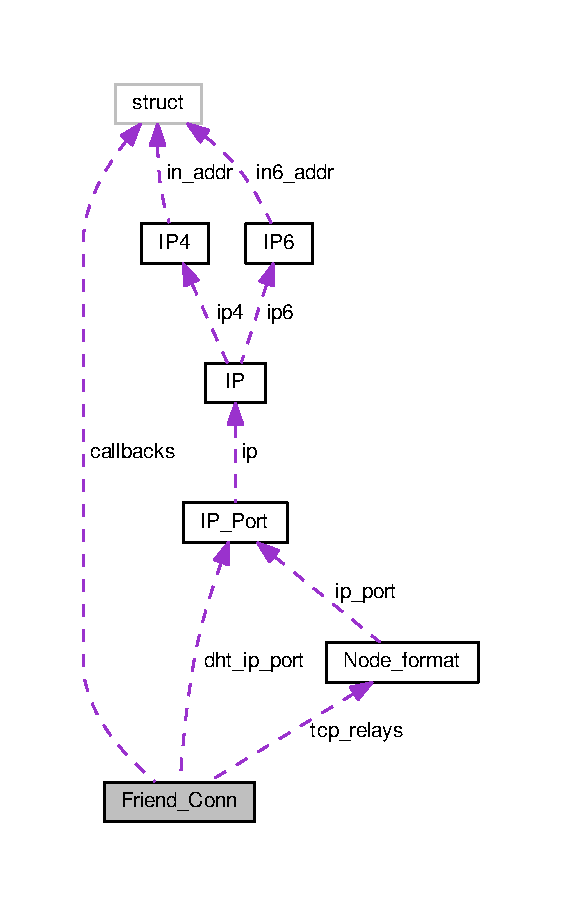
\includegraphics[width=270pt]{struct_friend___conn__coll__graph}
\end{center}
\end{figure}
\subsection*{Data Fields}
\begin{DoxyCompactItemize}
\item 
\hypertarget{struct_friend___conn_ade818037fd6c985038ff29656089758d}{uint8\+\_\+t {\bfseries status}}\label{struct_friend___conn_ade818037fd6c985038ff29656089758d}

\item 
\hypertarget{struct_friend___conn_a996dcaefa2a5954a199e2beb584c1feb}{uint8\+\_\+t {\bfseries real\+\_\+public\+\_\+key} \mbox{[}crypto\+\_\+box\+\_\+\+P\+U\+B\+L\+I\+C\+K\+E\+Y\+B\+Y\+T\+E\+S\mbox{]}}\label{struct_friend___conn_a996dcaefa2a5954a199e2beb584c1feb}

\item 
\hypertarget{struct_friend___conn_ab863a4d1023acff25635c1b4a36015a2}{uint8\+\_\+t {\bfseries dht\+\_\+temp\+\_\+pk} \mbox{[}crypto\+\_\+box\+\_\+\+P\+U\+B\+L\+I\+C\+K\+E\+Y\+B\+Y\+T\+E\+S\mbox{]}}\label{struct_friend___conn_ab863a4d1023acff25635c1b4a36015a2}

\item 
\hypertarget{struct_friend___conn_a1da451cf7bce45009c3ae38c003f2ed8}{uint16\+\_\+t {\bfseries dht\+\_\+lock}}\label{struct_friend___conn_a1da451cf7bce45009c3ae38c003f2ed8}

\item 
\hypertarget{struct_friend___conn_ace58c2ab8adca0a754bcd2527e88a9d2}{\hyperlink{struct_i_p___port}{I\+P\+\_\+\+Port} {\bfseries dht\+\_\+ip\+\_\+port}}\label{struct_friend___conn_ace58c2ab8adca0a754bcd2527e88a9d2}

\item 
\hypertarget{struct_friend___conn_a64eb95337c42cb30956ee42f7c42cf0e}{uint64\+\_\+t {\bfseries dht\+\_\+pk\+\_\+lastrecv}}\label{struct_friend___conn_a64eb95337c42cb30956ee42f7c42cf0e}

\item 
\hypertarget{struct_friend___conn_a1b4abfeab3eeeb285cfc69b1ac8d84bb}{uint64\+\_\+t {\bfseries dht\+\_\+ip\+\_\+port\+\_\+lastrecv}}\label{struct_friend___conn_a1b4abfeab3eeeb285cfc69b1ac8d84bb}

\item 
\hypertarget{struct_friend___conn_a009e6d32e21cc7fb0c8caded782e974b}{int {\bfseries onion\+\_\+friendnum}}\label{struct_friend___conn_a009e6d32e21cc7fb0c8caded782e974b}

\item 
\hypertarget{struct_friend___conn_a5ca114d88c26607a45883173f86c7c20}{int {\bfseries crypt\+\_\+connection\+\_\+id}}\label{struct_friend___conn_a5ca114d88c26607a45883173f86c7c20}

\item 
\hypertarget{struct_friend___conn_a5130c3c4a93050475770184608d61918}{uint64\+\_\+t {\bfseries ping\+\_\+lastrecv}}\label{struct_friend___conn_a5130c3c4a93050475770184608d61918}

\item 
\hypertarget{struct_friend___conn_a1625b76f8f5277e17545953d96b893fb}{uint64\+\_\+t {\bfseries ping\+\_\+lastsent}}\label{struct_friend___conn_a1625b76f8f5277e17545953d96b893fb}

\item 
\hypertarget{struct_friend___conn_aa5f9fa72527b8eafd6457864f32d2701}{uint64\+\_\+t {\bfseries share\+\_\+relays\+\_\+lastsent}}\label{struct_friend___conn_aa5f9fa72527b8eafd6457864f32d2701}

\item 
\hypertarget{struct_friend___conn_a213983130190a8281ab689630f0aee97}{\begin{tabbing}
xx\=xx\=xx\=xx\=xx\=xx\=xx\=xx\=xx\=\kill
struct \{\\
\>int($\ast$ {\bfseries status\_callback} )(void $\ast$object, int id, \\
\>\>uint8\_t status)\\
\>void $\ast$ {\bfseries status\_callback\_object}\\
\>int {\bfseries status\_callback\_id}\\
\>int($\ast$ {\bfseries data\_callback} )(void $\ast$object, int id, \\
\>\>uint8\_t $\ast$data, uint16\_t length)\\
\>void $\ast$ {\bfseries data\_callback\_object}\\
\>int {\bfseries data\_callback\_id}\\
\>int($\ast$ {\bfseries lossy\_data\_callback} )(void $\ast$object, int id, const \\
\>\>uint8\_t $\ast$data, uint16\_t length)\\
\>void $\ast$ {\bfseries lossy\_data\_callback\_object}\\
\>int {\bfseries lossy\_data\_callback\_id}\\
\} {\bfseries callbacks} \mbox{[}MAX\_FRIEND\_CONNECTION\_CALLBACKS\mbox{]}}\label{struct_friend___conn_a213983130190a8281ab689630f0aee97}
\\

\end{tabbing}\item 
\hypertarget{struct_friend___conn_a712c4c639bfc0f5a8616eead3e24ca4e}{uint16\+\_\+t {\bfseries lock\+\_\+count}}\label{struct_friend___conn_a712c4c639bfc0f5a8616eead3e24ca4e}

\item 
\hypertarget{struct_friend___conn_ae6c286282d15bfd5ceea7c2d8b19be5d}{\hyperlink{struct_node__format}{Node\+\_\+format} {\bfseries tcp\+\_\+relays} \mbox{[}F\+R\+I\+E\+N\+D\+\_\+\+M\+A\+X\+\_\+\+S\+T\+O\+R\+E\+D\+\_\+\+T\+C\+P\+\_\+\+R\+E\+L\+A\+Y\+S\mbox{]}}\label{struct_friend___conn_ae6c286282d15bfd5ceea7c2d8b19be5d}

\item 
\hypertarget{struct_friend___conn_aff5cc62447994133f0b5b15e11aa92ed}{uint16\+\_\+t {\bfseries tcp\+\_\+relay\+\_\+counter}}\label{struct_friend___conn_aff5cc62447994133f0b5b15e11aa92ed}

\item 
\hypertarget{struct_friend___conn_a4865ba9009fdee84e62a08fb92a59ab5}{\+\_\+\+Bool {\bfseries hosting\+\_\+tcp\+\_\+relay}}\label{struct_friend___conn_a4865ba9009fdee84e62a08fb92a59ab5}

\end{DoxyCompactItemize}


\subsection{Detailed Description}


Definition at line 66 of file friend\+\_\+connection.\+h.



The documentation for this struct was generated from the following file\+:\begin{DoxyCompactItemize}
\item 
toxcore/friend\+\_\+connection.\+h\end{DoxyCompactItemize}

\hypertarget{struct_friend___connections}{\section{Friend\+\_\+\+Connections Struct Reference}
\label{struct_friend___connections}\index{Friend\+\_\+\+Connections@{Friend\+\_\+\+Connections}}
}


Collaboration diagram for Friend\+\_\+\+Connections\+:
\nopagebreak
\begin{figure}[H]
\begin{center}
\leavevmode
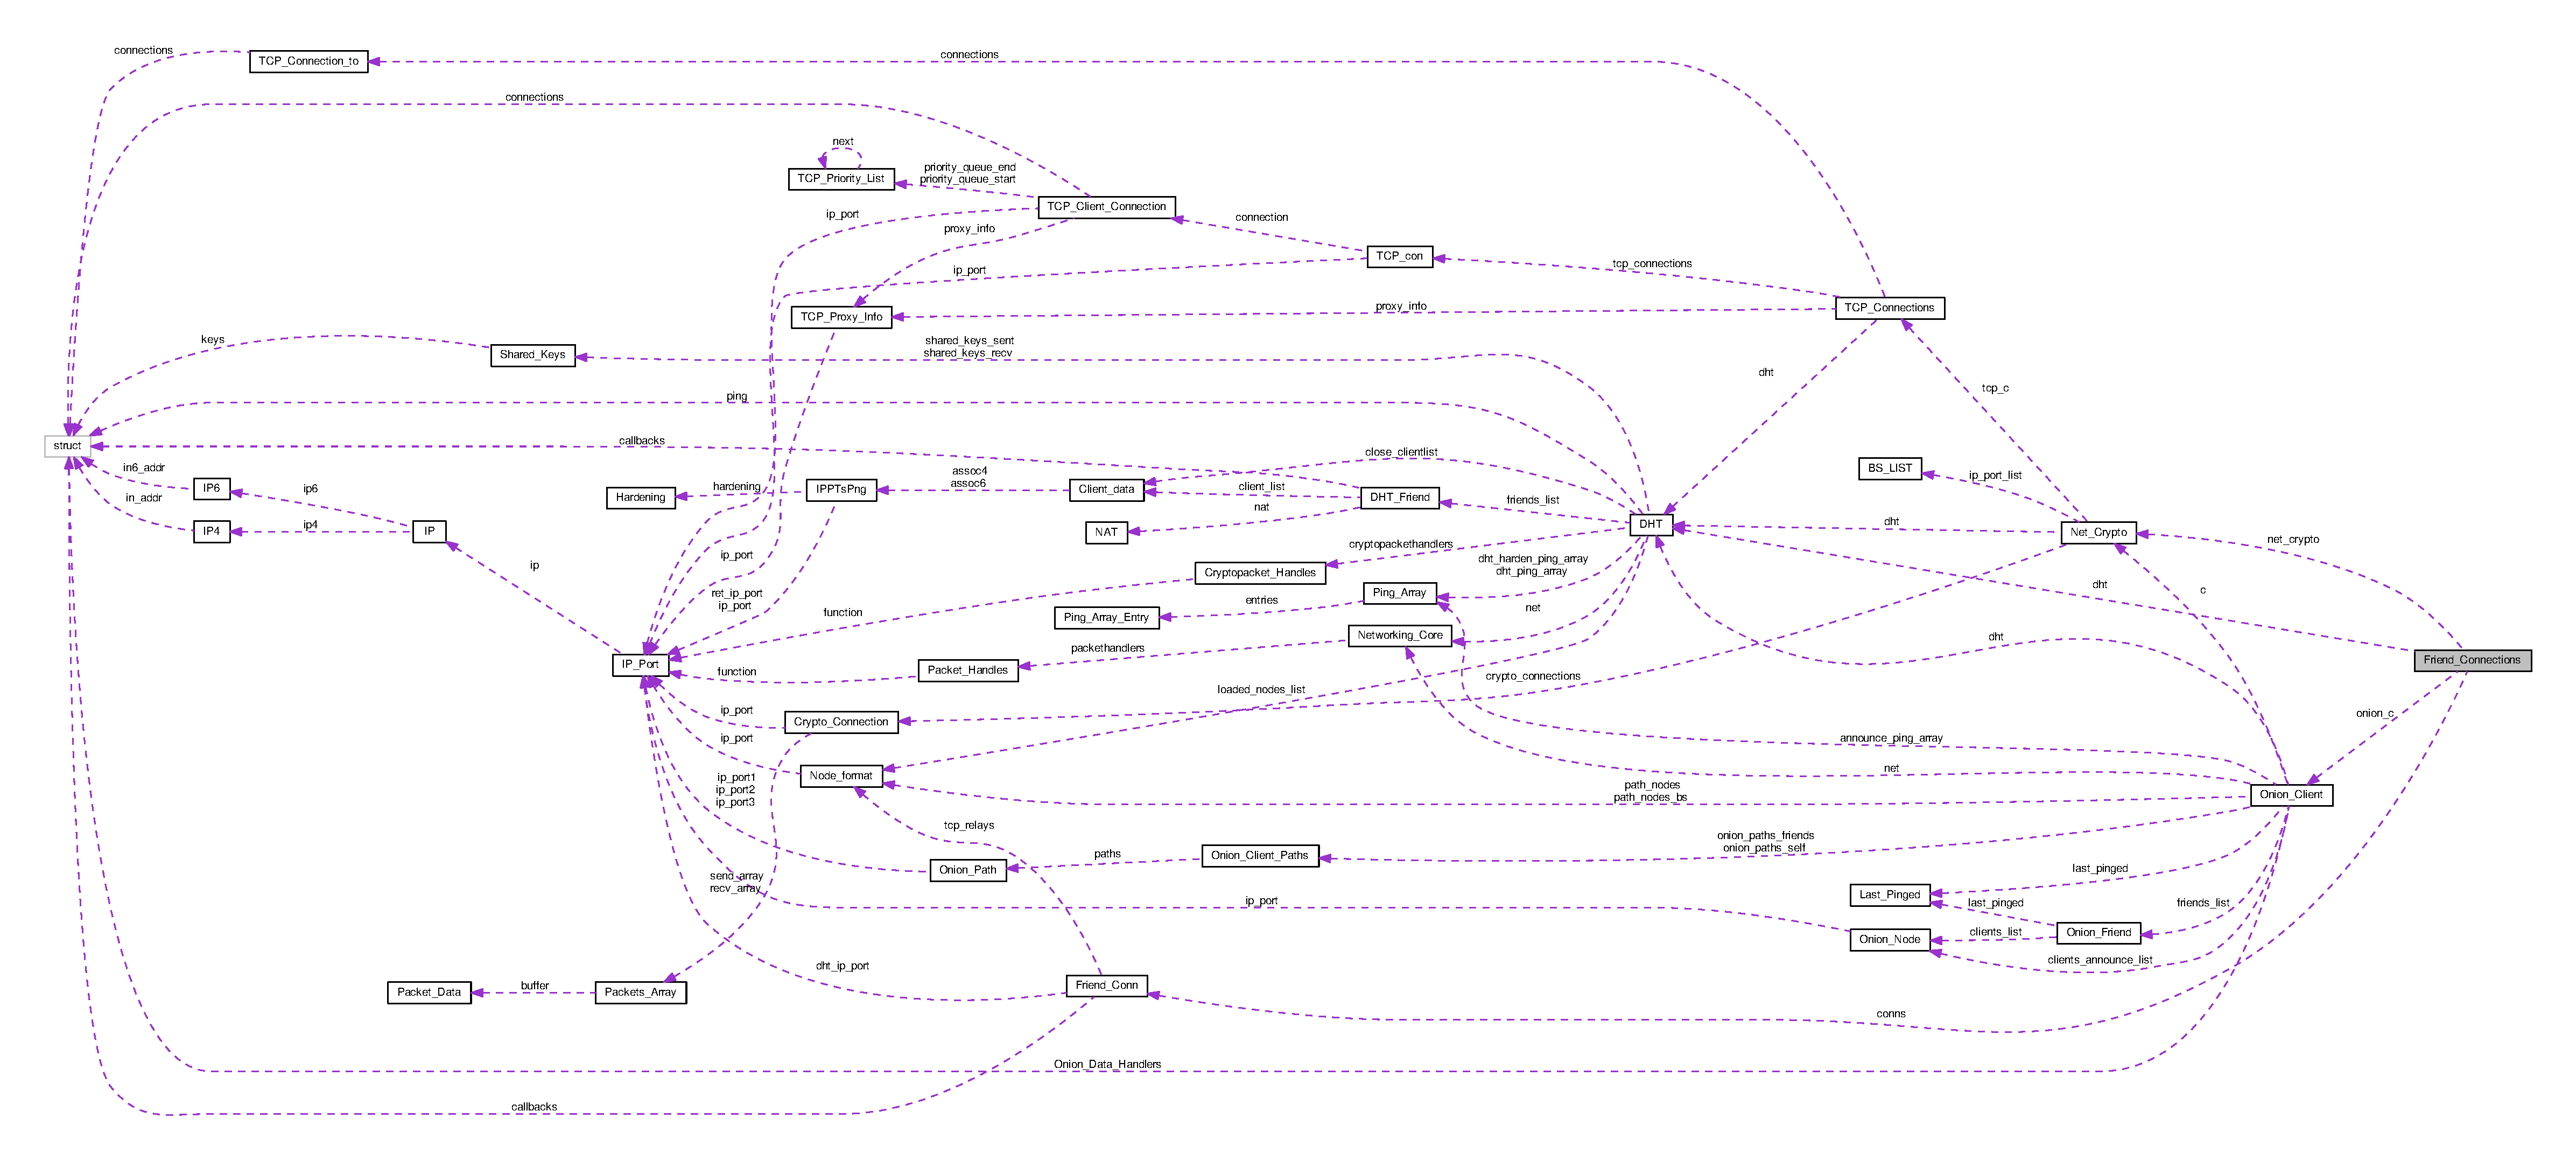
\includegraphics[width=350pt]{struct_friend___connections__coll__graph}
\end{center}
\end{figure}
\subsection*{Data Fields}
\begin{DoxyCompactItemize}
\item 
\hypertarget{struct_friend___connections_ab06a41217a1e9b5985555e19e088ae94}{\hyperlink{struct_net___crypto}{Net\+\_\+\+Crypto} $\ast$ {\bfseries net\+\_\+crypto}}\label{struct_friend___connections_ab06a41217a1e9b5985555e19e088ae94}

\item 
\hypertarget{struct_friend___connections_a8b3d6ce8745acc52695e252bdb1531b6}{\hyperlink{struct_d_h_t}{D\+H\+T} $\ast$ {\bfseries dht}}\label{struct_friend___connections_a8b3d6ce8745acc52695e252bdb1531b6}

\item 
\hypertarget{struct_friend___connections_ae202b81f9a2c2fa80fd310a0996795fc}{\hyperlink{struct_onion___client}{Onion\+\_\+\+Client} $\ast$ {\bfseries onion\+\_\+c}}\label{struct_friend___connections_ae202b81f9a2c2fa80fd310a0996795fc}

\item 
\hypertarget{struct_friend___connections_a2690adb6c61682af2e8592f53e9de9a0}{\hyperlink{struct_friend___conn}{Friend\+\_\+\+Conn} $\ast$ {\bfseries conns}}\label{struct_friend___connections_a2690adb6c61682af2e8592f53e9de9a0}

\item 
\hypertarget{struct_friend___connections_a81ac77652d6cc5071baca915581c5dfa}{uint32\+\_\+t {\bfseries num\+\_\+cons}}\label{struct_friend___connections_a81ac77652d6cc5071baca915581c5dfa}

\item 
\hypertarget{struct_friend___connections_a36e4f0e3167d9e95df5d7f83cbafa7fc}{int($\ast$ {\bfseries fr\+\_\+request\+\_\+callback} )(void $\ast$object, const uint8\+\_\+t $\ast$source\+\_\+pubkey, const uint8\+\_\+t $\ast$data, uint16\+\_\+t len)}\label{struct_friend___connections_a36e4f0e3167d9e95df5d7f83cbafa7fc}

\item 
\hypertarget{struct_friend___connections_abd31f2a386ec582b378de4fc3f05ea6c}{void $\ast$ {\bfseries fr\+\_\+request\+\_\+object}}\label{struct_friend___connections_abd31f2a386ec582b378de4fc3f05ea6c}

\item 
\hypertarget{struct_friend___connections_a4f77ba6531c78b4f6a2a46843d06cc26}{uint64\+\_\+t {\bfseries last\+\_\+\+L\+A\+Ndiscovery}}\label{struct_friend___connections_a4f77ba6531c78b4f6a2a46843d06cc26}

\end{DoxyCompactItemize}


\subsection{Detailed Description}


Definition at line 104 of file friend\+\_\+connection.\+h.



The documentation for this struct was generated from the following file\+:\begin{DoxyCompactItemize}
\item 
toxcore/friend\+\_\+connection.\+h\end{DoxyCompactItemize}

\hypertarget{struct_friend__request}{\section{Friend\+\_\+request Struct Reference}
\label{struct_friend__request}\index{Friend\+\_\+request@{Friend\+\_\+request}}
}
\subsection*{Data Fields}
\begin{DoxyCompactItemize}
\item 
uint8\+\_\+t \hyperlink{struct_friend__request_aca2bb72adf3445dbc7d501753fc2396d}{id} \mbox{[}\hyperlink{tox_8h_a6a25b8b522f6d65bacd1d84981b8c75c}{T\+O\+X\+\_\+\+P\+U\+B\+L\+I\+C\+\_\+\+K\+E\+Y\+\_\+\+S\+I\+Z\+E}\mbox{]}
\item 
uint8\+\_\+t \hyperlink{struct_friend__request_a41a8f1919b834fd7e1d1e48aa06c09a8}{accepted}
\end{DoxyCompactItemize}


\subsection{Detailed Description}


Definition at line 107 of file n\+Tox.\+c.



\subsection{Field Documentation}
\hypertarget{struct_friend__request_a41a8f1919b834fd7e1d1e48aa06c09a8}{\index{Friend\+\_\+request@{Friend\+\_\+request}!accepted@{accepted}}
\index{accepted@{accepted}!Friend\+\_\+request@{Friend\+\_\+request}}
\subsubsection[{accepted}]{\setlength{\rightskip}{0pt plus 5cm}uint8\+\_\+t accepted}}\label{struct_friend__request_a41a8f1919b834fd7e1d1e48aa06c09a8}


Definition at line 109 of file n\+Tox.\+c.



Referenced by line\+\_\+eval(), and print\+\_\+request().

\hypertarget{struct_friend__request_aca2bb72adf3445dbc7d501753fc2396d}{\index{Friend\+\_\+request@{Friend\+\_\+request}!id@{id}}
\index{id@{id}!Friend\+\_\+request@{Friend\+\_\+request}}
\subsubsection[{id}]{\setlength{\rightskip}{0pt plus 5cm}uint8\+\_\+t id\mbox{[}{\bf T\+O\+X\+\_\+\+P\+U\+B\+L\+I\+C\+\_\+\+K\+E\+Y\+\_\+\+S\+I\+Z\+E}\mbox{]}}}\label{struct_friend__request_aca2bb72adf3445dbc7d501753fc2396d}


Definition at line 108 of file n\+Tox.\+c.



The documentation for this struct was generated from the following file\+:\begin{DoxyCompactItemize}
\item 
testing/\hyperlink{n_tox_8c}{n\+Tox.\+c}\end{DoxyCompactItemize}

\hypertarget{struct_friend___requests}{\section{Friend\+\_\+\+Requests Struct Reference}
\label{struct_friend___requests}\index{Friend\+\_\+\+Requests@{Friend\+\_\+\+Requests}}
}


{\ttfamily \#include $<$friend\+\_\+requests.\+h$>$}

\subsection*{Data Fields}
\begin{DoxyCompactItemize}
\item 
uint32\+\_\+t \hyperlink{struct_friend___requests_a637ab08069536895c9a896c4ee9dcdf7}{nospam}
\item 
void($\ast$ \hyperlink{struct_friend___requests_a9d869a78e35e2af8312a3bec21dc7d0c}{handle\+\_\+friendrequest} )(void $\ast$, const uint8\+\_\+t $\ast$, const uint8\+\_\+t $\ast$, size\+\_\+t, void $\ast$)
\item 
uint8\+\_\+t \hyperlink{struct_friend___requests_aef7d18a109ced43f4cb3069083a91e69}{handle\+\_\+friendrequest\+\_\+isset}
\item 
void $\ast$ \hyperlink{struct_friend___requests_a21949251a7cb2ba8e6e3f973c8fdd01c}{handle\+\_\+friendrequest\+\_\+object}
\item 
void $\ast$ \hyperlink{struct_friend___requests_a59dcbf63199ca147db439e5ade631a81}{handle\+\_\+friendrequest\+\_\+userdata}
\item 
int($\ast$ \hyperlink{struct_friend___requests_a09cd55683f2075e72518e94efbcba2d5}{filter\+\_\+function} )(const uint8\+\_\+t $\ast$, void $\ast$)
\item 
void $\ast$ \hyperlink{struct_friend___requests_a52b17bf891c29cd0309d69ddf5be7e5e}{filter\+\_\+function\+\_\+userdata}
\item 
uint8\+\_\+t \hyperlink{struct_friend___requests_a68ddfbf4a697f40962f07c5608f394cf}{received\+\_\+requests} \mbox{[}\hyperlink{friend__requests_8h_adad74320175e7fbddd37ceecc6385b8a}{M\+A\+X\+\_\+\+R\+E\+C\+E\+I\+V\+E\+D\+\_\+\+S\+T\+O\+R\+E\+D}\mbox{]}\mbox{[}crypto\+\_\+box\+\_\+\+P\+U\+B\+L\+I\+C\+K\+E\+Y\+B\+Y\+T\+E\+S\mbox{]}
\item 
uint16\+\_\+t \hyperlink{struct_friend___requests_a0e318c112b35d57bd44f5a47b9e3f680}{received\+\_\+requests\+\_\+index}
\end{DoxyCompactItemize}


\subsection{Detailed Description}


Definition at line 31 of file friend\+\_\+requests.\+h.



\subsection{Field Documentation}
\hypertarget{struct_friend___requests_a09cd55683f2075e72518e94efbcba2d5}{\index{Friend\+\_\+\+Requests@{Friend\+\_\+\+Requests}!filter\+\_\+function@{filter\+\_\+function}}
\index{filter\+\_\+function@{filter\+\_\+function}!Friend\+\_\+\+Requests@{Friend\+\_\+\+Requests}}
\subsubsection[{filter\+\_\+function}]{\setlength{\rightskip}{0pt plus 5cm}int($\ast$ filter\+\_\+function)(const uint8\+\_\+t $\ast$, void $\ast$)}}\label{struct_friend___requests_a09cd55683f2075e72518e94efbcba2d5}


Definition at line 38 of file friend\+\_\+requests.\+h.



Referenced by friendreq\+\_\+handlepacket(), and set\+\_\+filter\+\_\+function().

\hypertarget{struct_friend___requests_a52b17bf891c29cd0309d69ddf5be7e5e}{\index{Friend\+\_\+\+Requests@{Friend\+\_\+\+Requests}!filter\+\_\+function\+\_\+userdata@{filter\+\_\+function\+\_\+userdata}}
\index{filter\+\_\+function\+\_\+userdata@{filter\+\_\+function\+\_\+userdata}!Friend\+\_\+\+Requests@{Friend\+\_\+\+Requests}}
\subsubsection[{filter\+\_\+function\+\_\+userdata}]{\setlength{\rightskip}{0pt plus 5cm}void$\ast$ filter\+\_\+function\+\_\+userdata}}\label{struct_friend___requests_a52b17bf891c29cd0309d69ddf5be7e5e}


Definition at line 39 of file friend\+\_\+requests.\+h.



Referenced by friendreq\+\_\+handlepacket(), and set\+\_\+filter\+\_\+function().

\hypertarget{struct_friend___requests_a9d869a78e35e2af8312a3bec21dc7d0c}{\index{Friend\+\_\+\+Requests@{Friend\+\_\+\+Requests}!handle\+\_\+friendrequest@{handle\+\_\+friendrequest}}
\index{handle\+\_\+friendrequest@{handle\+\_\+friendrequest}!Friend\+\_\+\+Requests@{Friend\+\_\+\+Requests}}
\subsubsection[{handle\+\_\+friendrequest}]{\setlength{\rightskip}{0pt plus 5cm}void($\ast$ handle\+\_\+friendrequest)(void $\ast$, const uint8\+\_\+t $\ast$, const uint8\+\_\+t $\ast$, size\+\_\+t, void $\ast$)}}\label{struct_friend___requests_a9d869a78e35e2af8312a3bec21dc7d0c}


Definition at line 33 of file friend\+\_\+requests.\+h.



Referenced by callback\+\_\+friendrequest(), and friendreq\+\_\+handlepacket().

\hypertarget{struct_friend___requests_aef7d18a109ced43f4cb3069083a91e69}{\index{Friend\+\_\+\+Requests@{Friend\+\_\+\+Requests}!handle\+\_\+friendrequest\+\_\+isset@{handle\+\_\+friendrequest\+\_\+isset}}
\index{handle\+\_\+friendrequest\+\_\+isset@{handle\+\_\+friendrequest\+\_\+isset}!Friend\+\_\+\+Requests@{Friend\+\_\+\+Requests}}
\subsubsection[{handle\+\_\+friendrequest\+\_\+isset}]{\setlength{\rightskip}{0pt plus 5cm}uint8\+\_\+t handle\+\_\+friendrequest\+\_\+isset}}\label{struct_friend___requests_aef7d18a109ced43f4cb3069083a91e69}


Definition at line 34 of file friend\+\_\+requests.\+h.



Referenced by callback\+\_\+friendrequest(), and friendreq\+\_\+handlepacket().

\hypertarget{struct_friend___requests_a21949251a7cb2ba8e6e3f973c8fdd01c}{\index{Friend\+\_\+\+Requests@{Friend\+\_\+\+Requests}!handle\+\_\+friendrequest\+\_\+object@{handle\+\_\+friendrequest\+\_\+object}}
\index{handle\+\_\+friendrequest\+\_\+object@{handle\+\_\+friendrequest\+\_\+object}!Friend\+\_\+\+Requests@{Friend\+\_\+\+Requests}}
\subsubsection[{handle\+\_\+friendrequest\+\_\+object}]{\setlength{\rightskip}{0pt plus 5cm}void$\ast$ handle\+\_\+friendrequest\+\_\+object}}\label{struct_friend___requests_a21949251a7cb2ba8e6e3f973c8fdd01c}


Definition at line 35 of file friend\+\_\+requests.\+h.



Referenced by callback\+\_\+friendrequest(), and friendreq\+\_\+handlepacket().

\hypertarget{struct_friend___requests_a59dcbf63199ca147db439e5ade631a81}{\index{Friend\+\_\+\+Requests@{Friend\+\_\+\+Requests}!handle\+\_\+friendrequest\+\_\+userdata@{handle\+\_\+friendrequest\+\_\+userdata}}
\index{handle\+\_\+friendrequest\+\_\+userdata@{handle\+\_\+friendrequest\+\_\+userdata}!Friend\+\_\+\+Requests@{Friend\+\_\+\+Requests}}
\subsubsection[{handle\+\_\+friendrequest\+\_\+userdata}]{\setlength{\rightskip}{0pt plus 5cm}void$\ast$ handle\+\_\+friendrequest\+\_\+userdata}}\label{struct_friend___requests_a59dcbf63199ca147db439e5ade631a81}


Definition at line 36 of file friend\+\_\+requests.\+h.



Referenced by callback\+\_\+friendrequest(), and friendreq\+\_\+handlepacket().

\hypertarget{struct_friend___requests_a637ab08069536895c9a896c4ee9dcdf7}{\index{Friend\+\_\+\+Requests@{Friend\+\_\+\+Requests}!nospam@{nospam}}
\index{nospam@{nospam}!Friend\+\_\+\+Requests@{Friend\+\_\+\+Requests}}
\subsubsection[{nospam}]{\setlength{\rightskip}{0pt plus 5cm}uint32\+\_\+t nospam}}\label{struct_friend___requests_a637ab08069536895c9a896c4ee9dcdf7}


Definition at line 32 of file friend\+\_\+requests.\+h.



Referenced by friendreq\+\_\+handlepacket(), get\+\_\+nospam(), and set\+\_\+nospam().

\hypertarget{struct_friend___requests_a68ddfbf4a697f40962f07c5608f394cf}{\index{Friend\+\_\+\+Requests@{Friend\+\_\+\+Requests}!received\+\_\+requests@{received\+\_\+requests}}
\index{received\+\_\+requests@{received\+\_\+requests}!Friend\+\_\+\+Requests@{Friend\+\_\+\+Requests}}
\subsubsection[{received\+\_\+requests}]{\setlength{\rightskip}{0pt plus 5cm}uint8\+\_\+t received\+\_\+requests\mbox{[}{\bf M\+A\+X\+\_\+\+R\+E\+C\+E\+I\+V\+E\+D\+\_\+\+S\+T\+O\+R\+E\+D}\mbox{]}\mbox{[}crypto\+\_\+box\+\_\+\+P\+U\+B\+L\+I\+C\+K\+E\+Y\+B\+Y\+T\+E\+S\mbox{]}}}\label{struct_friend___requests_a68ddfbf4a697f40962f07c5608f394cf}


Definition at line 46 of file friend\+\_\+requests.\+h.



Referenced by addto\+\_\+receivedlist(), remove\+\_\+request\+\_\+received(), and request\+\_\+received().

\hypertarget{struct_friend___requests_a0e318c112b35d57bd44f5a47b9e3f680}{\index{Friend\+\_\+\+Requests@{Friend\+\_\+\+Requests}!received\+\_\+requests\+\_\+index@{received\+\_\+requests\+\_\+index}}
\index{received\+\_\+requests\+\_\+index@{received\+\_\+requests\+\_\+index}!Friend\+\_\+\+Requests@{Friend\+\_\+\+Requests}}
\subsubsection[{received\+\_\+requests\+\_\+index}]{\setlength{\rightskip}{0pt plus 5cm}uint16\+\_\+t received\+\_\+requests\+\_\+index}}\label{struct_friend___requests_a0e318c112b35d57bd44f5a47b9e3f680}


Definition at line 47 of file friend\+\_\+requests.\+h.



Referenced by addto\+\_\+receivedlist().



The documentation for this struct was generated from the following file\+:\begin{DoxyCompactItemize}
\item 
toxcore/\hyperlink{friend__requests_8h}{friend\+\_\+requests.\+h}\end{DoxyCompactItemize}

\hypertarget{struct_group___audio___packet}{\section{Group\+\_\+\+Audio\+\_\+\+Packet Struct Reference}
\label{struct_group___audio___packet}\index{Group\+\_\+\+Audio\+\_\+\+Packet@{Group\+\_\+\+Audio\+\_\+\+Packet}}
}
\subsection*{Data Fields}
\begin{DoxyCompactItemize}
\item 
\hypertarget{struct_group___audio___packet_afe208c7dec97b8f61e08094e61bf096e}{uint16\+\_\+t {\bfseries sequnum}}\label{struct_group___audio___packet_afe208c7dec97b8f61e08094e61bf096e}

\item 
\hypertarget{struct_group___audio___packet_a1892eba2086d12ac2b09005aeb09ea3b}{uint16\+\_\+t {\bfseries length}}\label{struct_group___audio___packet_a1892eba2086d12ac2b09005aeb09ea3b}

\item 
\hypertarget{struct_group___audio___packet_a5c239a1bb87b52b0f1d6d68c4749cd2a}{uint8\+\_\+t {\bfseries data} \mbox{[}$\,$\mbox{]}}\label{struct_group___audio___packet_a5c239a1bb87b52b0f1d6d68c4749cd2a}

\end{DoxyCompactItemize}


\subsection{Detailed Description}


Definition at line 32 of file group.\+c.



The documentation for this struct was generated from the following file\+:\begin{DoxyCompactItemize}
\item 
toxav/group.\+c\end{DoxyCompactItemize}

\hypertarget{struct_group___a_v}{\section{Group\+\_\+\+A\+V Struct Reference}
\label{struct_group___a_v}\index{Group\+\_\+\+A\+V@{Group\+\_\+\+A\+V}}
}


Collaboration diagram for Group\+\_\+\+A\+V\+:
\nopagebreak
\begin{figure}[H]
\begin{center}
\leavevmode
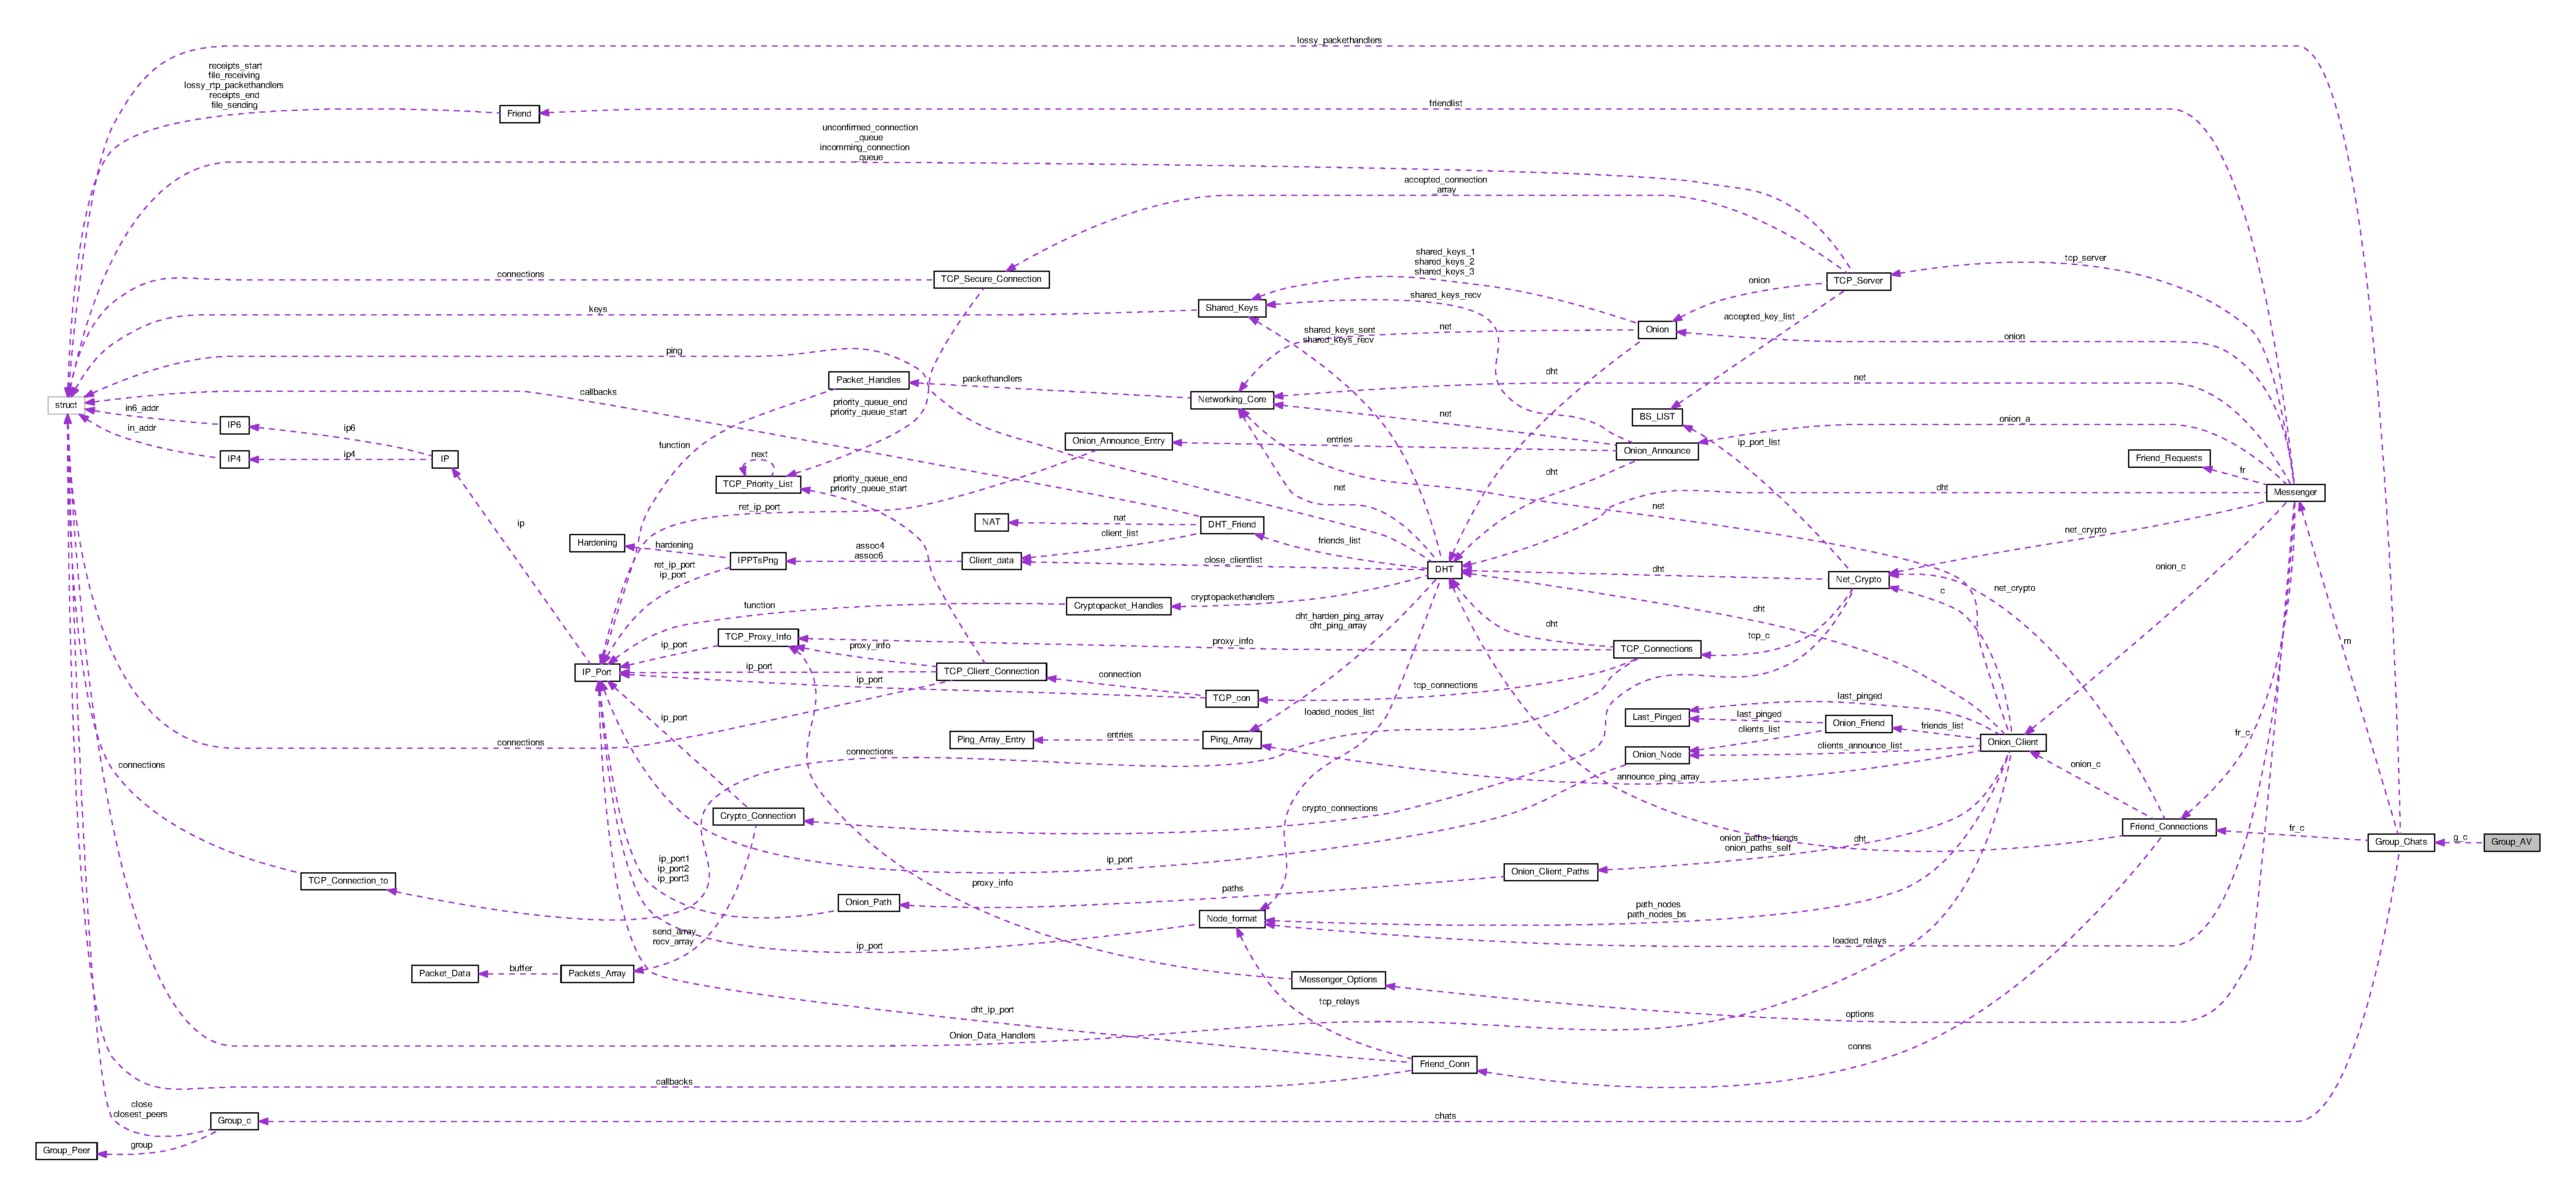
\includegraphics[width=350pt]{struct_group___a_v__coll__graph}
\end{center}
\end{figure}
\subsection*{Data Fields}
\begin{DoxyCompactItemize}
\item 
\hypertarget{struct_group___a_v_a0220ceb497e4d7ffcbd301959cbfaf26}{\hyperlink{struct_group___chats}{Group\+\_\+\+Chats} $\ast$ {\bfseries g\+\_\+c}}\label{struct_group___a_v_a0220ceb497e4d7ffcbd301959cbfaf26}

\item 
\hypertarget{struct_group___a_v_a8c1fa3d73f3426ba5cac83857c390ebc}{Opus\+Encoder $\ast$ {\bfseries audio\+\_\+encoder}}\label{struct_group___a_v_a8c1fa3d73f3426ba5cac83857c390ebc}

\item 
\hypertarget{struct_group___a_v_a7b6aa0a517a158485dccd6ce0a916e0e}{unsigned int {\bfseries audio\+\_\+channels}}\label{struct_group___a_v_a7b6aa0a517a158485dccd6ce0a916e0e}

\item 
\hypertarget{struct_group___a_v_a0562d75f5e3bb5cce19ab1eae44fdaac}{unsigned int {\bfseries audio\+\_\+sample\+\_\+rate}}\label{struct_group___a_v_a0562d75f5e3bb5cce19ab1eae44fdaac}

\item 
\hypertarget{struct_group___a_v_a1e39921527f07befd08d913c63b397a9}{unsigned int {\bfseries audio\+\_\+bitrate}}\label{struct_group___a_v_a1e39921527f07befd08d913c63b397a9}

\item 
\hypertarget{struct_group___a_v_a4e6b863a96b5fadfc86cc2ef353c76db}{uint16\+\_\+t {\bfseries audio\+\_\+sequnum}}\label{struct_group___a_v_a4e6b863a96b5fadfc86cc2ef353c76db}

\item 
\hypertarget{struct_group___a_v_a2ae2d081bbdd51062bcb82ea4a55eec5}{void($\ast$ {\bfseries audio\+\_\+data} )(\hyperlink{struct_messenger}{Messenger} $\ast$m, int groupnumber, int peernumber, const int16\+\_\+t $\ast$pcm, unsigned int samples, uint8\+\_\+t channels, unsigned int sample\+\_\+rate, void $\ast$userdata)}\label{struct_group___a_v_a2ae2d081bbdd51062bcb82ea4a55eec5}

\item 
\hypertarget{struct_group___a_v_afd0ffb02780e738d4c0a10ab833b7834}{void $\ast$ {\bfseries userdata}}\label{struct_group___a_v_afd0ffb02780e738d4c0a10ab833b7834}

\end{DoxyCompactItemize}


\subsection{Detailed Description}


Definition at line 152 of file group.\+c.



The documentation for this struct was generated from the following file\+:\begin{DoxyCompactItemize}
\item 
toxav/group.\+c\end{DoxyCompactItemize}

\hypertarget{struct_group__c}{\section{Group\+\_\+c Struct Reference}
\label{struct_group__c}\index{Group\+\_\+c@{Group\+\_\+c}}
}


Collaboration diagram for Group\+\_\+c\+:\nopagebreak
\begin{figure}[H]
\begin{center}
\leavevmode
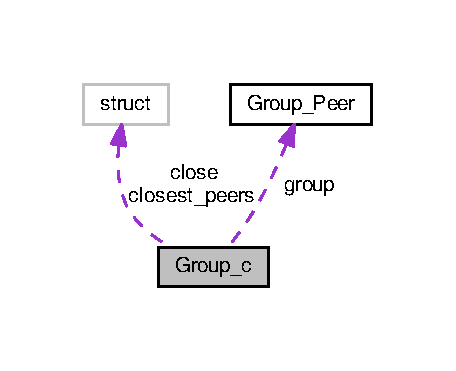
\includegraphics[width=219pt]{struct_group__c__coll__graph}
\end{center}
\end{figure}
\subsection*{Data Fields}
\begin{DoxyCompactItemize}
\item 
\hypertarget{struct_group__c_ade818037fd6c985038ff29656089758d}{uint8\+\_\+t {\bfseries status}}\label{struct_group__c_ade818037fd6c985038ff29656089758d}

\item 
\hypertarget{struct_group__c_a1f68599dc07252599a98f6d044a184e9}{\hyperlink{struct_group___peer}{Group\+\_\+\+Peer} $\ast$ {\bfseries group}}\label{struct_group__c_a1f68599dc07252599a98f6d044a184e9}

\item 
\hypertarget{struct_group__c_a6c81294c96de8914431dbf825934b528}{uint32\+\_\+t {\bfseries numpeers}}\label{struct_group__c_a6c81294c96de8914431dbf825934b528}

\item 
\hypertarget{struct_group__c_a6c24608383f70ad37f70307f492e3abc}{\begin{tabbing}
xx\=xx\=xx\=xx\=xx\=xx\=xx\=xx\=xx\=\kill
struct \{\\
\>uint8\_t {\bfseries type}\\
\>uint8\_t {\bfseries closest}\\
\>uint32\_t {\bfseries number}\\
\>uint16\_t {\bfseries group\_number}\\
\} {\bfseries close} \mbox{[}MAX\_GROUP\_CONNECTIONS\mbox{]}}\label{struct_group__c_a6c24608383f70ad37f70307f492e3abc}
\\

\end{tabbing}\item 
\hypertarget{struct_group__c_ab42b4c90d81ac99b968c3edd1e21d706}{uint8\+\_\+t {\bfseries real\+\_\+pk} \mbox{[}crypto\+\_\+box\+\_\+\+P\+U\+B\+L\+I\+C\+K\+E\+Y\+B\+Y\+T\+E\+S\mbox{]}}\label{struct_group__c_ab42b4c90d81ac99b968c3edd1e21d706}

\item 
\hypertarget{struct_group__c_a8987e8417b5a1a5bc11ba79885c12590}{\begin{tabbing}
xx\=xx\=xx\=xx\=xx\=xx\=xx\=xx\=xx\=\kill
struct \{\\
\>uint8\_t {\bfseries entry}\\
\>uint8\_t {\bfseries real\_pk} \mbox{[}crypto\_box\_PUBLICKEYBYTES\mbox{]}\\
\>uint8\_t {\bfseries temp\_pk} \mbox{[}crypto\_box\_PUBLICKEYBYTES\mbox{]}\\
\} {\bfseries closest\_peers} \mbox{[}DESIRED\_CLOSE\_CONNECTIONS\mbox{]}}\label{struct_group__c_a8987e8417b5a1a5bc11ba79885c12590}
\\

\end{tabbing}\item 
\hypertarget{struct_group__c_aab3e81d63c7e7e9e693aa0f5fb574fa4}{uint8\+\_\+t {\bfseries changed}}\label{struct_group__c_aab3e81d63c7e7e9e693aa0f5fb574fa4}

\item 
\hypertarget{struct_group__c_a590984b7f44686ea4892ffa2651b0cda}{uint8\+\_\+t {\bfseries identifier} \mbox{[}G\+R\+O\+U\+P\+\_\+\+I\+D\+E\+N\+T\+I\+F\+I\+E\+R\+\_\+\+L\+E\+N\+G\+T\+H\mbox{]}}\label{struct_group__c_a590984b7f44686ea4892ffa2651b0cda}

\item 
\hypertarget{struct_group__c_a9ace0499016685340a1f3009a7aa01e0}{uint8\+\_\+t {\bfseries title} \mbox{[}M\+A\+X\+\_\+\+N\+A\+M\+E\+\_\+\+L\+E\+N\+G\+T\+H\mbox{]}}\label{struct_group__c_a9ace0499016685340a1f3009a7aa01e0}

\item 
\hypertarget{struct_group__c_ac32d4f2bb9021dfa0b7ce5f9537412d7}{uint8\+\_\+t {\bfseries title\+\_\+len}}\label{struct_group__c_ac32d4f2bb9021dfa0b7ce5f9537412d7}

\item 
\hypertarget{struct_group__c_a1ecee33a5d6309a114891c3fb740b66c}{uint32\+\_\+t {\bfseries message\+\_\+number}}\label{struct_group__c_a1ecee33a5d6309a114891c3fb740b66c}

\item 
\hypertarget{struct_group__c_acc475ae1ff50d43f08a2cc920a5d2ae5}{uint16\+\_\+t {\bfseries lossy\+\_\+message\+\_\+number}}\label{struct_group__c_acc475ae1ff50d43f08a2cc920a5d2ae5}

\item 
\hypertarget{struct_group__c_a264348ec1f724e05464ca97b7c432817}{uint16\+\_\+t {\bfseries peer\+\_\+number}}\label{struct_group__c_a264348ec1f724e05464ca97b7c432817}

\item 
\hypertarget{struct_group__c_a0137c615a93acf73b05a3d710231dd3d}{uint64\+\_\+t {\bfseries last\+\_\+sent\+\_\+ping}}\label{struct_group__c_a0137c615a93acf73b05a3d710231dd3d}

\item 
\hypertarget{struct_group__c_a50fa99a57ee7c9280fc90b7c33d760d0}{int {\bfseries number\+\_\+joined}}\label{struct_group__c_a50fa99a57ee7c9280fc90b7c33d760d0}

\item 
\hypertarget{struct_group__c_a077376d12464f945e2414d5499c79b3f}{void $\ast$ {\bfseries object}}\label{struct_group__c_a077376d12464f945e2414d5499c79b3f}

\item 
\hypertarget{struct_group__c_a218cd2e97bdb682b90f72faa6eb08576}{void($\ast$ {\bfseries peer\+\_\+on\+\_\+join} )(void $\ast$, int, int)}\label{struct_group__c_a218cd2e97bdb682b90f72faa6eb08576}

\item 
\hypertarget{struct_group__c_a7a79b984292a5ea1f68aca7b73067370}{void($\ast$ {\bfseries peer\+\_\+on\+\_\+leave} )(void $\ast$, int, int, void $\ast$)}\label{struct_group__c_a7a79b984292a5ea1f68aca7b73067370}

\item 
\hypertarget{struct_group__c_a43df326d671eb30dd294d5d71d3cd09c}{void($\ast$ {\bfseries group\+\_\+on\+\_\+delete} )(void $\ast$, int)}\label{struct_group__c_a43df326d671eb30dd294d5d71d3cd09c}

\end{DoxyCompactItemize}


\subsection{Detailed Description}


Definition at line 71 of file group.\+h.



The documentation for this struct was generated from the following file\+:\begin{DoxyCompactItemize}
\item 
toxcore/group.\+h\end{DoxyCompactItemize}

\hypertarget{struct_group___chats}{\section{Group\+\_\+\+Chats Struct Reference}
\label{struct_group___chats}\index{Group\+\_\+\+Chats@{Group\+\_\+\+Chats}}
}


{\ttfamily \#include $<$group.\+h$>$}



Collaboration diagram for Group\+\_\+\+Chats\+:
\nopagebreak
\begin{figure}[H]
\begin{center}
\leavevmode
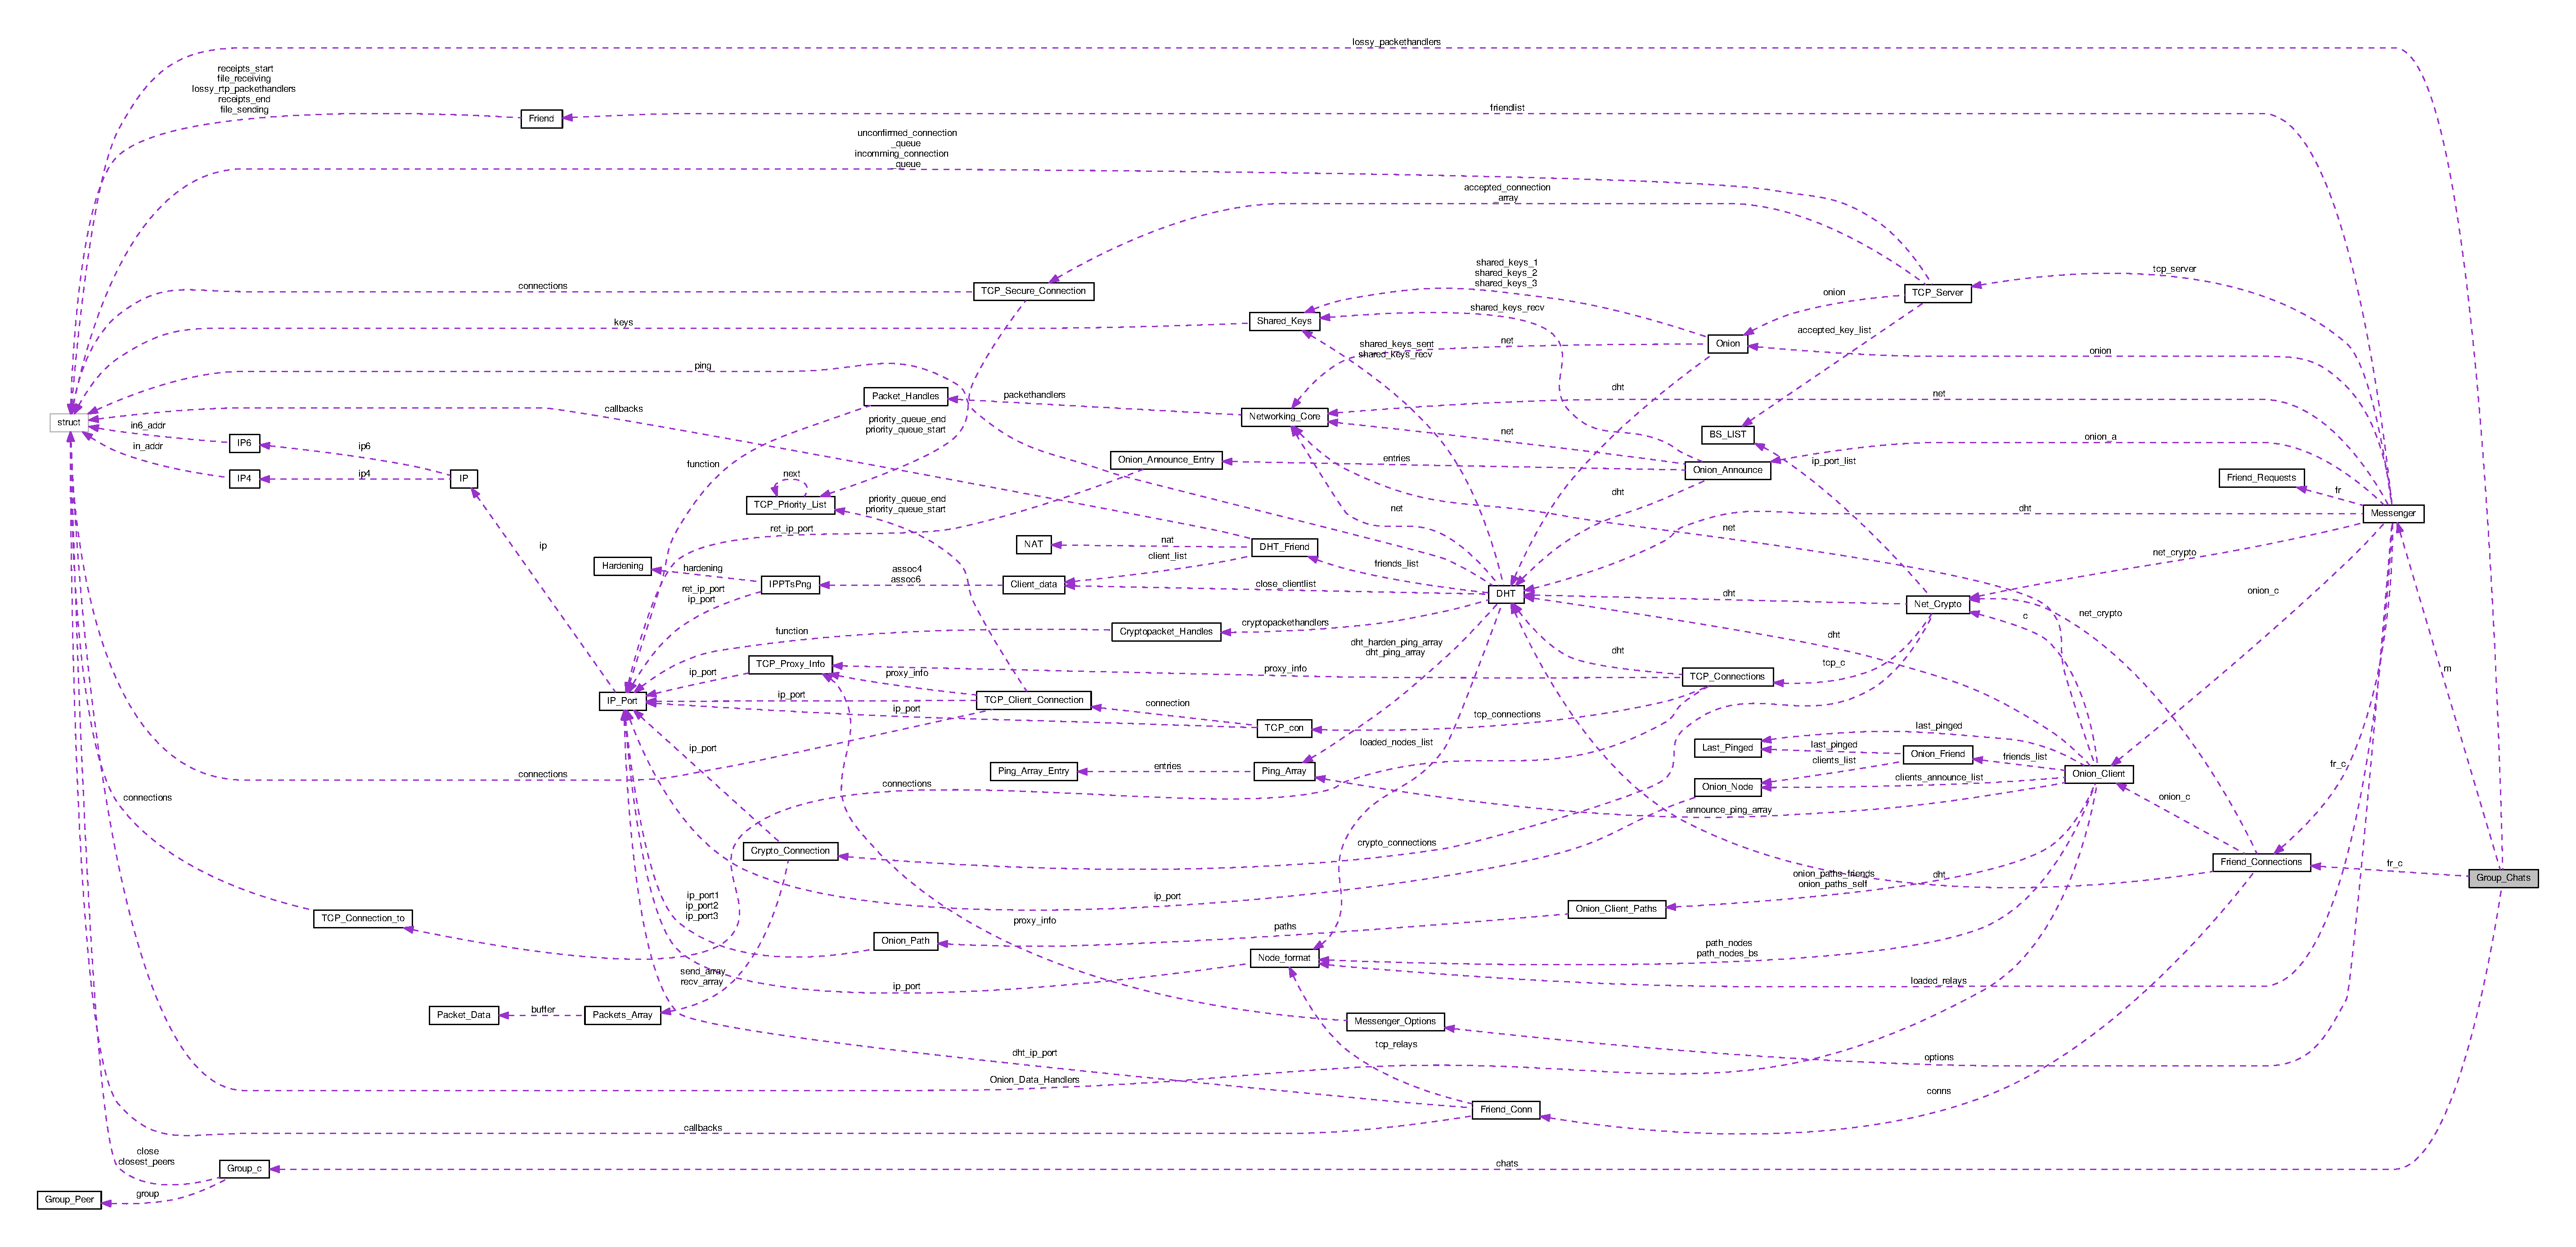
\includegraphics[width=350pt]{df/d3a/struct_group___chats__coll__graph}
\end{center}
\end{figure}
\subsection*{Data Fields}
\begin{DoxyCompactItemize}
\item 
\hyperlink{struct_messenger}{Messenger} $\ast$ \hyperlink{struct_group___chats_aea6eb6c7c30a659f1b0dee83eaf03ea2}{m}
\item 
\hyperlink{struct_friend___connections}{Friend\+\_\+\+Connections} $\ast$ \hyperlink{struct_group___chats_ae26eb43a606fff20fe70209d051c40f9}{fr\+\_\+c}
\item 
\hyperlink{struct_group__c}{Group\+\_\+c} $\ast$ \hyperlink{struct_group___chats_a2a89a032b3d68d95f8cbecf4ecec9e74}{chats}
\item 
uint32\+\_\+t \hyperlink{struct_group___chats_af6dc2bcdf8d71e0faaa6601befa94d9b}{num\+\_\+chats}
\item 
void($\ast$ \hyperlink{struct_group___chats_a4ff3e6778b94fb9425a4b36572a0bf8b}{invite\+\_\+callback} )(\hyperlink{struct_messenger}{Messenger} $\ast$\hyperlink{struct_group___chats_aea6eb6c7c30a659f1b0dee83eaf03ea2}{m}, int32\+\_\+t, uint8\+\_\+t, const uint8\+\_\+t $\ast$, uint16\+\_\+t, void $\ast$)
\item 
void $\ast$ \hyperlink{struct_group___chats_a4a640f20c34159b06875274fedf9dc69}{invite\+\_\+callback\+\_\+userdata}
\item 
void($\ast$ \hyperlink{struct_group___chats_a0f49e6a148c90647f5280d35d0f7a9d0}{message\+\_\+callback} )(\hyperlink{struct_messenger}{Messenger} $\ast$\hyperlink{struct_group___chats_aea6eb6c7c30a659f1b0dee83eaf03ea2}{m}, int, int, const uint8\+\_\+t $\ast$, uint16\+\_\+t, void $\ast$)
\item 
void $\ast$ \hyperlink{struct_group___chats_a593c4aa670d5dc3d9fcd842fb8d5a6fe}{message\+\_\+callback\+\_\+userdata}
\item 
void($\ast$ \hyperlink{struct_group___chats_a61996fdab7da709944de726b88872d61}{action\+\_\+callback} )(\hyperlink{struct_messenger}{Messenger} $\ast$\hyperlink{struct_group___chats_aea6eb6c7c30a659f1b0dee83eaf03ea2}{m}, int, int, const uint8\+\_\+t $\ast$, uint16\+\_\+t, void $\ast$)
\item 
void $\ast$ \hyperlink{struct_group___chats_ab8194101242ca87c3ee0fd11f7717569}{action\+\_\+callback\+\_\+userdata}
\item 
void($\ast$ \hyperlink{struct_group___chats_a3f11f69cf6d4e6d1ed57b5306b097baf}{peer\+\_\+namelistchange} )(\hyperlink{struct_messenger}{Messenger} $\ast$\hyperlink{struct_group___chats_aea6eb6c7c30a659f1b0dee83eaf03ea2}{m}, int, int, uint8\+\_\+t, void $\ast$)
\item 
void $\ast$ \hyperlink{struct_group___chats_a4c6b98ab07da7e69ecb7ae245f765984}{group\+\_\+namelistchange\+\_\+userdata}
\item 
void($\ast$ \hyperlink{struct_group___chats_a3a2940882c161941fd7f3274064bd594}{title\+\_\+callback} )(\hyperlink{struct_messenger}{Messenger} $\ast$\hyperlink{struct_group___chats_aea6eb6c7c30a659f1b0dee83eaf03ea2}{m}, int, int, const uint8\+\_\+t $\ast$, uint8\+\_\+t, void $\ast$)
\item 
void $\ast$ \hyperlink{struct_group___chats_a75c386ae84b59f8f38e02cd0f841ba8b}{title\+\_\+callback\+\_\+userdata}
\item 
\begin{tabbing}
xx\=xx\=xx\=xx\=xx\=xx\=xx\=xx\=xx\=\kill
struct \{\\
\>int($\ast$ \hyperlink{struct_group___chats_acbfbbdaa6d4201766377ac50de985ae9}{function} )(void $\ast$, int, int, void \\
\>\>$\ast$, const uint8\_t $\ast$, uint16\_t)\\
\} \hyperlink{struct_group___chats_a3630aa7993bdd216d40637826a92649f}{lossy\_packethandlers} \mbox{[}256\mbox{]}\\

\end{tabbing}\end{DoxyCompactItemize}


\subsection{Detailed Description}


Definition at line 112 of file group.\+h.



\subsection{Field Documentation}
\hypertarget{struct_group___chats_a61996fdab7da709944de726b88872d61}{\index{Group\+\_\+\+Chats@{Group\+\_\+\+Chats}!action\+\_\+callback@{action\+\_\+callback}}
\index{action\+\_\+callback@{action\+\_\+callback}!Group\+\_\+\+Chats@{Group\+\_\+\+Chats}}
\subsubsection[{action\+\_\+callback}]{\setlength{\rightskip}{0pt plus 5cm}void($\ast$ action\+\_\+callback)({\bf Messenger} $\ast${\bf m}, int, int, const uint8\+\_\+t $\ast$, uint16\+\_\+t, void $\ast$)}}\label{struct_group___chats_a61996fdab7da709944de726b88872d61}


Definition at line 123 of file group.\+h.



Referenced by g\+\_\+callback\+\_\+group\+\_\+action(), and handle\+\_\+message\+\_\+packet\+\_\+group().

\hypertarget{struct_group___chats_ab8194101242ca87c3ee0fd11f7717569}{\index{Group\+\_\+\+Chats@{Group\+\_\+\+Chats}!action\+\_\+callback\+\_\+userdata@{action\+\_\+callback\+\_\+userdata}}
\index{action\+\_\+callback\+\_\+userdata@{action\+\_\+callback\+\_\+userdata}!Group\+\_\+\+Chats@{Group\+\_\+\+Chats}}
\subsubsection[{action\+\_\+callback\+\_\+userdata}]{\setlength{\rightskip}{0pt plus 5cm}void$\ast$ action\+\_\+callback\+\_\+userdata}}\label{struct_group___chats_ab8194101242ca87c3ee0fd11f7717569}


Definition at line 124 of file group.\+h.



Referenced by g\+\_\+callback\+\_\+group\+\_\+action(), and handle\+\_\+message\+\_\+packet\+\_\+group().

\hypertarget{struct_group___chats_a2a89a032b3d68d95f8cbecf4ecec9e74}{\index{Group\+\_\+\+Chats@{Group\+\_\+\+Chats}!chats@{chats}}
\index{chats@{chats}!Group\+\_\+\+Chats@{Group\+\_\+\+Chats}}
\subsubsection[{chats}]{\setlength{\rightskip}{0pt plus 5cm}{\bf Group\+\_\+c}$\ast$ chats}}\label{struct_group___chats_a2a89a032b3d68d95f8cbecf4ecec9e74}


Definition at line 116 of file group.\+h.



Referenced by add\+\_\+groupchat(), copy\+\_\+chatlist(), count\+\_\+chatlist(), create\+\_\+group\+\_\+chat(), get\+\_\+group\+\_\+c(), get\+\_\+group\+\_\+num(), groupnumber\+\_\+not\+\_\+valid(), join\+\_\+groupchat(), realloc\+\_\+groupchats(), and wipe\+\_\+group\+\_\+chat().

\hypertarget{struct_group___chats_ae26eb43a606fff20fe70209d051c40f9}{\index{Group\+\_\+\+Chats@{Group\+\_\+\+Chats}!fr\+\_\+c@{fr\+\_\+c}}
\index{fr\+\_\+c@{fr\+\_\+c}!Group\+\_\+\+Chats@{Group\+\_\+\+Chats}}
\subsubsection[{fr\+\_\+c}]{\setlength{\rightskip}{0pt plus 5cm}{\bf Friend\+\_\+\+Connections}$\ast$ fr\+\_\+c}}\label{struct_group___chats_ae26eb43a606fff20fe70209d051c40f9}


Definition at line 114 of file group.\+h.



Referenced by add\+\_\+conn\+\_\+to\+\_\+groupchat(), connect\+\_\+to\+\_\+closest(), del\+\_\+groupchat(), delpeer(), handle\+\_\+direct\+\_\+packet(), handle\+\_\+friend\+\_\+invite\+\_\+packet(), handle\+\_\+packet\+\_\+online(), new\+\_\+groupchats(), remove\+\_\+close\+\_\+conn(), send\+\_\+lossy\+\_\+all\+\_\+close(), send\+\_\+message\+\_\+all\+\_\+close(), send\+\_\+peer\+\_\+kill(), send\+\_\+peer\+\_\+query(), send\+\_\+peers(), and set\+\_\+conns\+\_\+type\+\_\+close().

\hypertarget{struct_group___chats_acbfbbdaa6d4201766377ac50de985ae9}{\index{Group\+\_\+\+Chats@{Group\+\_\+\+Chats}!function@{function}}
\index{function@{function}!Group\+\_\+\+Chats@{Group\+\_\+\+Chats}}
\subsubsection[{function}]{\setlength{\rightskip}{0pt plus 5cm}int($\ast$ function)(void $\ast$, int, int, void $\ast$, const uint8\+\_\+t $\ast$, uint16\+\_\+t)}}\label{struct_group___chats_acbfbbdaa6d4201766377ac50de985ae9}


Definition at line 131 of file group.\+h.



Referenced by group\+\_\+lossy\+\_\+packet\+\_\+registerhandler(), and handle\+\_\+lossy().

\hypertarget{struct_group___chats_a4c6b98ab07da7e69ecb7ae245f765984}{\index{Group\+\_\+\+Chats@{Group\+\_\+\+Chats}!group\+\_\+namelistchange\+\_\+userdata@{group\+\_\+namelistchange\+\_\+userdata}}
\index{group\+\_\+namelistchange\+\_\+userdata@{group\+\_\+namelistchange\+\_\+userdata}!Group\+\_\+\+Chats@{Group\+\_\+\+Chats}}
\subsubsection[{group\+\_\+namelistchange\+\_\+userdata}]{\setlength{\rightskip}{0pt plus 5cm}void$\ast$ group\+\_\+namelistchange\+\_\+userdata}}\label{struct_group___chats_a4c6b98ab07da7e69ecb7ae245f765984}


Definition at line 126 of file group.\+h.



Referenced by addpeer(), delpeer(), g\+\_\+callback\+\_\+group\+\_\+namelistchange(), and setnick().

\hypertarget{struct_group___chats_a4ff3e6778b94fb9425a4b36572a0bf8b}{\index{Group\+\_\+\+Chats@{Group\+\_\+\+Chats}!invite\+\_\+callback@{invite\+\_\+callback}}
\index{invite\+\_\+callback@{invite\+\_\+callback}!Group\+\_\+\+Chats@{Group\+\_\+\+Chats}}
\subsubsection[{invite\+\_\+callback}]{\setlength{\rightskip}{0pt plus 5cm}void($\ast$ invite\+\_\+callback)({\bf Messenger} $\ast${\bf m}, int32\+\_\+t, uint8\+\_\+t, const uint8\+\_\+t $\ast$, uint16\+\_\+t, void $\ast$)}}\label{struct_group___chats_a4ff3e6778b94fb9425a4b36572a0bf8b}


Definition at line 119 of file group.\+h.



Referenced by g\+\_\+callback\+\_\+group\+\_\+invite(), and handle\+\_\+friend\+\_\+invite\+\_\+packet().

\hypertarget{struct_group___chats_a4a640f20c34159b06875274fedf9dc69}{\index{Group\+\_\+\+Chats@{Group\+\_\+\+Chats}!invite\+\_\+callback\+\_\+userdata@{invite\+\_\+callback\+\_\+userdata}}
\index{invite\+\_\+callback\+\_\+userdata@{invite\+\_\+callback\+\_\+userdata}!Group\+\_\+\+Chats@{Group\+\_\+\+Chats}}
\subsubsection[{invite\+\_\+callback\+\_\+userdata}]{\setlength{\rightskip}{0pt plus 5cm}void$\ast$ invite\+\_\+callback\+\_\+userdata}}\label{struct_group___chats_a4a640f20c34159b06875274fedf9dc69}


Definition at line 120 of file group.\+h.



Referenced by g\+\_\+callback\+\_\+group\+\_\+invite(), and handle\+\_\+friend\+\_\+invite\+\_\+packet().

\hypertarget{struct_group___chats_a3630aa7993bdd216d40637826a92649f}{\index{Group\+\_\+\+Chats@{Group\+\_\+\+Chats}!lossy\+\_\+packethandlers@{lossy\+\_\+packethandlers}}
\index{lossy\+\_\+packethandlers@{lossy\+\_\+packethandlers}!Group\+\_\+\+Chats@{Group\+\_\+\+Chats}}
\subsubsection[{lossy\+\_\+packethandlers}]{\setlength{\rightskip}{0pt plus 5cm}struct \{ ... \}   lossy\+\_\+packethandlers\mbox{[}256\mbox{]}}}\label{struct_group___chats_a3630aa7993bdd216d40637826a92649f}


Referenced by group\+\_\+lossy\+\_\+packet\+\_\+registerhandler(), and handle\+\_\+lossy().

\hypertarget{struct_group___chats_aea6eb6c7c30a659f1b0dee83eaf03ea2}{\index{Group\+\_\+\+Chats@{Group\+\_\+\+Chats}!m@{m}}
\index{m@{m}!Group\+\_\+\+Chats@{Group\+\_\+\+Chats}}
\subsubsection[{m}]{\setlength{\rightskip}{0pt plus 5cm}{\bf Messenger}$\ast$ m}}\label{struct_group___chats_aea6eb6c7c30a659f1b0dee83eaf03ea2}


Definition at line 113 of file group.\+h.



Referenced by add\+\_\+conn\+\_\+to\+\_\+groupchat(), add\+\_\+groupchat(), addpeer(), decode\+\_\+audio\+\_\+packet(), delpeer(), handle\+\_\+message\+\_\+packet\+\_\+group(), handle\+\_\+send\+\_\+peers(), invite\+\_\+friend(), join\+\_\+groupchat(), kill\+\_\+groupchats(), new\+\_\+groupchats(), send\+\_\+name\+\_\+all\+\_\+groups(), setnick(), and settitle().

\hypertarget{struct_group___chats_a0f49e6a148c90647f5280d35d0f7a9d0}{\index{Group\+\_\+\+Chats@{Group\+\_\+\+Chats}!message\+\_\+callback@{message\+\_\+callback}}
\index{message\+\_\+callback@{message\+\_\+callback}!Group\+\_\+\+Chats@{Group\+\_\+\+Chats}}
\subsubsection[{message\+\_\+callback}]{\setlength{\rightskip}{0pt plus 5cm}void($\ast$ message\+\_\+callback)({\bf Messenger} $\ast${\bf m}, int, int, const uint8\+\_\+t $\ast$, uint16\+\_\+t, void $\ast$)}}\label{struct_group___chats_a0f49e6a148c90647f5280d35d0f7a9d0}


Definition at line 121 of file group.\+h.



Referenced by g\+\_\+callback\+\_\+group\+\_\+message(), and handle\+\_\+message\+\_\+packet\+\_\+group().

\hypertarget{struct_group___chats_a593c4aa670d5dc3d9fcd842fb8d5a6fe}{\index{Group\+\_\+\+Chats@{Group\+\_\+\+Chats}!message\+\_\+callback\+\_\+userdata@{message\+\_\+callback\+\_\+userdata}}
\index{message\+\_\+callback\+\_\+userdata@{message\+\_\+callback\+\_\+userdata}!Group\+\_\+\+Chats@{Group\+\_\+\+Chats}}
\subsubsection[{message\+\_\+callback\+\_\+userdata}]{\setlength{\rightskip}{0pt plus 5cm}void$\ast$ message\+\_\+callback\+\_\+userdata}}\label{struct_group___chats_a593c4aa670d5dc3d9fcd842fb8d5a6fe}


Definition at line 122 of file group.\+h.



Referenced by g\+\_\+callback\+\_\+group\+\_\+message(), and handle\+\_\+message\+\_\+packet\+\_\+group().

\hypertarget{struct_group___chats_af6dc2bcdf8d71e0faaa6601befa94d9b}{\index{Group\+\_\+\+Chats@{Group\+\_\+\+Chats}!num\+\_\+chats@{num\+\_\+chats}}
\index{num\+\_\+chats@{num\+\_\+chats}!Group\+\_\+\+Chats@{Group\+\_\+\+Chats}}
\subsubsection[{num\+\_\+chats}]{\setlength{\rightskip}{0pt plus 5cm}uint32\+\_\+t num\+\_\+chats}}\label{struct_group___chats_af6dc2bcdf8d71e0faaa6601befa94d9b}


Definition at line 117 of file group.\+h.



Referenced by copy\+\_\+chatlist(), count\+\_\+chatlist(), create\+\_\+group\+\_\+chat(), do\+\_\+groupchats(), get\+\_\+group\+\_\+num(), groupnumber\+\_\+not\+\_\+valid(), kill\+\_\+groupchats(), send\+\_\+name\+\_\+all\+\_\+groups(), set\+\_\+conns\+\_\+status\+\_\+groups(), and wipe\+\_\+group\+\_\+chat().

\hypertarget{struct_group___chats_a3f11f69cf6d4e6d1ed57b5306b097baf}{\index{Group\+\_\+\+Chats@{Group\+\_\+\+Chats}!peer\+\_\+namelistchange@{peer\+\_\+namelistchange}}
\index{peer\+\_\+namelistchange@{peer\+\_\+namelistchange}!Group\+\_\+\+Chats@{Group\+\_\+\+Chats}}
\subsubsection[{peer\+\_\+namelistchange}]{\setlength{\rightskip}{0pt plus 5cm}void($\ast$ peer\+\_\+namelistchange)({\bf Messenger} $\ast${\bf m}, int, int, uint8\+\_\+t, void $\ast$)}}\label{struct_group___chats_a3f11f69cf6d4e6d1ed57b5306b097baf}


Definition at line 125 of file group.\+h.



Referenced by addpeer(), delpeer(), g\+\_\+callback\+\_\+group\+\_\+namelistchange(), and setnick().

\hypertarget{struct_group___chats_a3a2940882c161941fd7f3274064bd594}{\index{Group\+\_\+\+Chats@{Group\+\_\+\+Chats}!title\+\_\+callback@{title\+\_\+callback}}
\index{title\+\_\+callback@{title\+\_\+callback}!Group\+\_\+\+Chats@{Group\+\_\+\+Chats}}
\subsubsection[{title\+\_\+callback}]{\setlength{\rightskip}{0pt plus 5cm}void($\ast$ title\+\_\+callback)({\bf Messenger} $\ast${\bf m}, int, int, const uint8\+\_\+t $\ast$, uint8\+\_\+t, void $\ast$)}}\label{struct_group___chats_a3a2940882c161941fd7f3274064bd594}


Definition at line 127 of file group.\+h.



Referenced by g\+\_\+callback\+\_\+group\+\_\+title(), and settitle().

\hypertarget{struct_group___chats_a75c386ae84b59f8f38e02cd0f841ba8b}{\index{Group\+\_\+\+Chats@{Group\+\_\+\+Chats}!title\+\_\+callback\+\_\+userdata@{title\+\_\+callback\+\_\+userdata}}
\index{title\+\_\+callback\+\_\+userdata@{title\+\_\+callback\+\_\+userdata}!Group\+\_\+\+Chats@{Group\+\_\+\+Chats}}
\subsubsection[{title\+\_\+callback\+\_\+userdata}]{\setlength{\rightskip}{0pt plus 5cm}void$\ast$ title\+\_\+callback\+\_\+userdata}}\label{struct_group___chats_a75c386ae84b59f8f38e02cd0f841ba8b}


Definition at line 128 of file group.\+h.



Referenced by g\+\_\+callback\+\_\+group\+\_\+title(), and settitle().



The documentation for this struct was generated from the following file\+:\begin{DoxyCompactItemize}
\item 
toxcore/\hyperlink{toxcore_2group_8h}{group.\+h}\end{DoxyCompactItemize}

\hypertarget{struct_group___jitter_buffer}{\section{Group\+\_\+\+Jitter\+Buffer Struct Reference}
\label{struct_group___jitter_buffer}\index{Group\+\_\+\+Jitter\+Buffer@{Group\+\_\+\+Jitter\+Buffer}}
}


Collaboration diagram for Group\+\_\+\+Jitter\+Buffer\+:
\nopagebreak
\begin{figure}[H]
\begin{center}
\leavevmode
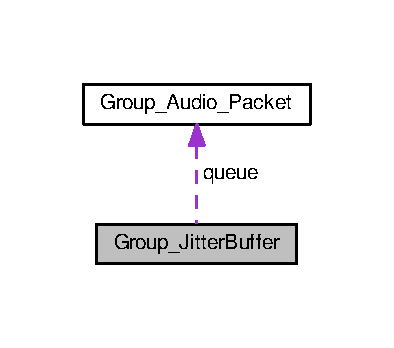
\includegraphics[width=189pt]{d1/d1d/struct_group___jitter_buffer__coll__graph}
\end{center}
\end{figure}
\subsection*{Data Fields}
\begin{DoxyCompactItemize}
\item 
\hyperlink{struct_group___audio___packet}{Group\+\_\+\+Audio\+\_\+\+Packet} $\ast$$\ast$ \hyperlink{struct_group___jitter_buffer_a9829940d971aa22eb04b318876afb018}{queue}
\item 
uint32\+\_\+t \hyperlink{struct_group___jitter_buffer_ab2c6b258f02add8fdf4cfc7c371dd772}{size}
\item 
uint32\+\_\+t \hyperlink{struct_group___jitter_buffer_a391c992c66c3e5540265a85ec2b9216a}{capacity}
\item 
uint16\+\_\+t \hyperlink{struct_group___jitter_buffer_a12c8099ac87952580dd090215e02728c}{bottom}
\item 
uint16\+\_\+t \hyperlink{struct_group___jitter_buffer_a0c235a6df98714bb18538fc0afc5bad1}{top}
\item 
uint64\+\_\+t \hyperlink{struct_group___jitter_buffer_abec0d4ef82ac14ce49e34eff86392f02}{last\+\_\+queued\+\_\+time}
\end{DoxyCompactItemize}


\subsection{Detailed Description}


Definition at line 38 of file group.\+c.



\subsection{Field Documentation}
\hypertarget{struct_group___jitter_buffer_a12c8099ac87952580dd090215e02728c}{\index{Group\+\_\+\+Jitter\+Buffer@{Group\+\_\+\+Jitter\+Buffer}!bottom@{bottom}}
\index{bottom@{bottom}!Group\+\_\+\+Jitter\+Buffer@{Group\+\_\+\+Jitter\+Buffer}}
\subsubsection[{bottom}]{\setlength{\rightskip}{0pt plus 5cm}uint16\+\_\+t bottom}}\label{struct_group___jitter_buffer_a12c8099ac87952580dd090215e02728c}


Definition at line 42 of file group.\+c.



Referenced by clear\+\_\+queue(), dequeue(), and queue().

\hypertarget{struct_group___jitter_buffer_a391c992c66c3e5540265a85ec2b9216a}{\index{Group\+\_\+\+Jitter\+Buffer@{Group\+\_\+\+Jitter\+Buffer}!capacity@{capacity}}
\index{capacity@{capacity}!Group\+\_\+\+Jitter\+Buffer@{Group\+\_\+\+Jitter\+Buffer}}
\subsubsection[{capacity}]{\setlength{\rightskip}{0pt plus 5cm}uint32\+\_\+t capacity}}\label{struct_group___jitter_buffer_a391c992c66c3e5540265a85ec2b9216a}


Definition at line 41 of file group.\+c.



Referenced by create\+\_\+queue(), dequeue(), and queue().

\hypertarget{struct_group___jitter_buffer_abec0d4ef82ac14ce49e34eff86392f02}{\index{Group\+\_\+\+Jitter\+Buffer@{Group\+\_\+\+Jitter\+Buffer}!last\+\_\+queued\+\_\+time@{last\+\_\+queued\+\_\+time}}
\index{last\+\_\+queued\+\_\+time@{last\+\_\+queued\+\_\+time}!Group\+\_\+\+Jitter\+Buffer@{Group\+\_\+\+Jitter\+Buffer}}
\subsubsection[{last\+\_\+queued\+\_\+time}]{\setlength{\rightskip}{0pt plus 5cm}uint64\+\_\+t last\+\_\+queued\+\_\+time}}\label{struct_group___jitter_buffer_abec0d4ef82ac14ce49e34eff86392f02}


Definition at line 44 of file group.\+c.



Referenced by queue().

\hypertarget{struct_group___jitter_buffer_a9829940d971aa22eb04b318876afb018}{\index{Group\+\_\+\+Jitter\+Buffer@{Group\+\_\+\+Jitter\+Buffer}!queue@{queue}}
\index{queue@{queue}!Group\+\_\+\+Jitter\+Buffer@{Group\+\_\+\+Jitter\+Buffer}}
\subsubsection[{queue}]{\setlength{\rightskip}{0pt plus 5cm}{\bf Group\+\_\+\+Audio\+\_\+\+Packet}$\ast$$\ast$ queue}}\label{struct_group___jitter_buffer_a9829940d971aa22eb04b318876afb018}


Definition at line 39 of file group.\+c.



Referenced by clear\+\_\+queue(), create\+\_\+queue(), dequeue(), queue(), and terminate\+\_\+queue().

\hypertarget{struct_group___jitter_buffer_ab2c6b258f02add8fdf4cfc7c371dd772}{\index{Group\+\_\+\+Jitter\+Buffer@{Group\+\_\+\+Jitter\+Buffer}!size@{size}}
\index{size@{size}!Group\+\_\+\+Jitter\+Buffer@{Group\+\_\+\+Jitter\+Buffer}}
\subsubsection[{size}]{\setlength{\rightskip}{0pt plus 5cm}uint32\+\_\+t size}}\label{struct_group___jitter_buffer_ab2c6b258f02add8fdf4cfc7c371dd772}


Definition at line 40 of file group.\+c.



Referenced by clear\+\_\+queue(), create\+\_\+queue(), dequeue(), and queue().

\hypertarget{struct_group___jitter_buffer_a0c235a6df98714bb18538fc0afc5bad1}{\index{Group\+\_\+\+Jitter\+Buffer@{Group\+\_\+\+Jitter\+Buffer}!top@{top}}
\index{top@{top}!Group\+\_\+\+Jitter\+Buffer@{Group\+\_\+\+Jitter\+Buffer}}
\subsubsection[{top}]{\setlength{\rightskip}{0pt plus 5cm}uint16\+\_\+t top}}\label{struct_group___jitter_buffer_a0c235a6df98714bb18538fc0afc5bad1}


Definition at line 43 of file group.\+c.



Referenced by clear\+\_\+queue(), dequeue(), and queue().



The documentation for this struct was generated from the following file\+:\begin{DoxyCompactItemize}
\item 
toxav/\hyperlink{toxav_2group_8c}{group.\+c}\end{DoxyCompactItemize}

\hypertarget{struct_group___peer}{\section{Group\+\_\+\+Peer Struct Reference}
\label{struct_group___peer}\index{Group\+\_\+\+Peer@{Group\+\_\+\+Peer}}
}
\subsection*{Data Fields}
\begin{DoxyCompactItemize}
\item 
\hypertarget{struct_group___peer_ab42b4c90d81ac99b968c3edd1e21d706}{uint8\+\_\+t {\bfseries real\+\_\+pk} \mbox{[}crypto\+\_\+box\+\_\+\+P\+U\+B\+L\+I\+C\+K\+E\+Y\+B\+Y\+T\+E\+S\mbox{]}}\label{struct_group___peer_ab42b4c90d81ac99b968c3edd1e21d706}

\item 
\hypertarget{struct_group___peer_a46affbcc202b25e96fd1f5238e9e97e0}{uint8\+\_\+t {\bfseries temp\+\_\+pk} \mbox{[}crypto\+\_\+box\+\_\+\+P\+U\+B\+L\+I\+C\+K\+E\+Y\+B\+Y\+T\+E\+S\mbox{]}}\label{struct_group___peer_a46affbcc202b25e96fd1f5238e9e97e0}

\item 
\hypertarget{struct_group___peer_a03706feea89530a7ac78082fc79ed8fc}{uint64\+\_\+t {\bfseries last\+\_\+recv}}\label{struct_group___peer_a03706feea89530a7ac78082fc79ed8fc}

\item 
\hypertarget{struct_group___peer_a1a221b969812bb7c384b0eb23fb1012d}{uint32\+\_\+t {\bfseries last\+\_\+message\+\_\+number}}\label{struct_group___peer_a1a221b969812bb7c384b0eb23fb1012d}

\item 
\hypertarget{struct_group___peer_ae7cf3fd18e321fab5a711e72622301b9}{uint8\+\_\+t {\bfseries nick} \mbox{[}M\+A\+X\+\_\+\+N\+A\+M\+E\+\_\+\+L\+E\+N\+G\+T\+H\mbox{]}}\label{struct_group___peer_ae7cf3fd18e321fab5a711e72622301b9}

\item 
\hypertarget{struct_group___peer_aa316280abcd8913a502b56397dd13e23}{uint8\+\_\+t {\bfseries nick\+\_\+len}}\label{struct_group___peer_aa316280abcd8913a502b56397dd13e23}

\item 
\hypertarget{struct_group___peer_a264348ec1f724e05464ca97b7c432817}{uint16\+\_\+t {\bfseries peer\+\_\+number}}\label{struct_group___peer_a264348ec1f724e05464ca97b7c432817}

\item 
\hypertarget{struct_group___peer_acf8dd69bcbe4de0b5a2b78803925994d}{uint8\+\_\+t {\bfseries recv\+\_\+lossy} \mbox{[}M\+A\+X\+\_\+\+L\+O\+S\+S\+Y\+\_\+\+C\+O\+U\+N\+T\mbox{]}}\label{struct_group___peer_acf8dd69bcbe4de0b5a2b78803925994d}

\item 
\hypertarget{struct_group___peer_ae3d9bdf641a1085fcb1bde6ec076b37d}{uint16\+\_\+t {\bfseries bottom\+\_\+lossy\+\_\+number}}\label{struct_group___peer_ae3d9bdf641a1085fcb1bde6ec076b37d}

\item 
\hypertarget{struct_group___peer_a9af1180e5be1617fd013dee9ce29bf24}{uint16\+\_\+t {\bfseries top\+\_\+lossy\+\_\+number}}\label{struct_group___peer_a9af1180e5be1617fd013dee9ce29bf24}

\item 
\hypertarget{struct_group___peer_a077376d12464f945e2414d5499c79b3f}{void $\ast$ {\bfseries object}}\label{struct_group___peer_a077376d12464f945e2414d5499c79b3f}

\end{DoxyCompactItemize}


\subsection{Detailed Description}


Definition at line 43 of file group.\+h.



The documentation for this struct was generated from the following file\+:\begin{DoxyCompactItemize}
\item 
toxcore/group.\+h\end{DoxyCompactItemize}

\hypertarget{struct_group___peer___a_v}{\section{Group\+\_\+\+Peer\+\_\+\+A\+V Struct Reference}
\label{struct_group___peer___a_v}\index{Group\+\_\+\+Peer\+\_\+\+A\+V@{Group\+\_\+\+Peer\+\_\+\+A\+V}}
}


Collaboration diagram for Group\+\_\+\+Peer\+\_\+\+A\+V\+:
\nopagebreak
\begin{figure}[H]
\begin{center}
\leavevmode
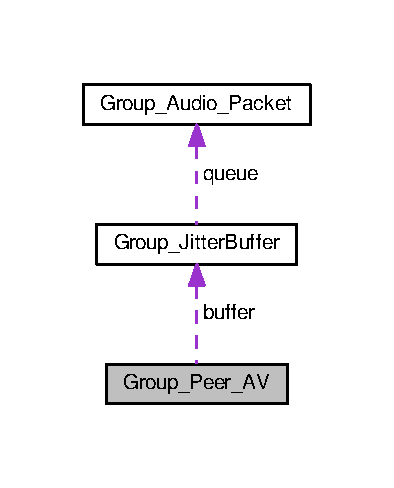
\includegraphics[width=189pt]{struct_group___peer___a_v__coll__graph}
\end{center}
\end{figure}
\subsection*{Data Fields}
\begin{DoxyCompactItemize}
\item 
\hypertarget{struct_group___peer___a_v_a6552b703c2e3958d1e030416f2893b27}{\hyperlink{struct_group___jitter_buffer}{Group\+\_\+\+Jitter\+Buffer} $\ast$ {\bfseries buffer}}\label{struct_group___peer___a_v_a6552b703c2e3958d1e030416f2893b27}

\item 
\hypertarget{struct_group___peer___a_v_a3b9ee5ac4c354a3e31a8acf7aa1a1b6c}{Opus\+Decoder $\ast$ {\bfseries audio\+\_\+decoder}}\label{struct_group___peer___a_v_a3b9ee5ac4c354a3e31a8acf7aa1a1b6c}

\item 
\hypertarget{struct_group___peer___a_v_afe1ef0788c8c4a05e136d1b00245138e}{int {\bfseries decoder\+\_\+channels}}\label{struct_group___peer___a_v_afe1ef0788c8c4a05e136d1b00245138e}

\item 
\hypertarget{struct_group___peer___a_v_af679faefa170266e24bc2af9b5a0161e}{unsigned int {\bfseries last\+\_\+packet\+\_\+samples}}\label{struct_group___peer___a_v_af679faefa170266e24bc2af9b5a0161e}

\end{DoxyCompactItemize}


\subsection{Detailed Description}


Definition at line 165 of file group.\+c.



The documentation for this struct was generated from the following file\+:\begin{DoxyCompactItemize}
\item 
toxav/group.\+c\end{DoxyCompactItemize}

\hypertarget{struct_hardening}{\section{Hardening Struct Reference}
\label{struct_hardening}\index{Hardening@{Hardening}}
}
\subsection*{Data Fields}
\begin{DoxyCompactItemize}
\item 
\hypertarget{struct_hardening_a3bc4c156861571ceca55275d95f6221b}{uint8\+\_\+t {\bfseries routes\+\_\+requests\+\_\+ok}}\label{struct_hardening_a3bc4c156861571ceca55275d95f6221b}

\item 
\hypertarget{struct_hardening_a55d6293fa06a8c4aa24e70706409b060}{uint64\+\_\+t {\bfseries routes\+\_\+requests\+\_\+timestamp}}\label{struct_hardening_a55d6293fa06a8c4aa24e70706409b060}

\item 
\hypertarget{struct_hardening_a7584df55876ac376c81e898ee9330252}{uint8\+\_\+t {\bfseries routes\+\_\+requests\+\_\+pingedid} \mbox{[}C\+L\+I\+E\+N\+T\+\_\+\+I\+D\+\_\+\+S\+I\+Z\+E\mbox{]}}\label{struct_hardening_a7584df55876ac376c81e898ee9330252}

\item 
\hypertarget{struct_hardening_a11158e002f3685f4044a759680636c08}{uint8\+\_\+t {\bfseries send\+\_\+nodes\+\_\+ok}}\label{struct_hardening_a11158e002f3685f4044a759680636c08}

\item 
\hypertarget{struct_hardening_ab15e3d8f0b33943a6978fac3cde4d1a2}{uint64\+\_\+t {\bfseries send\+\_\+nodes\+\_\+timestamp}}\label{struct_hardening_ab15e3d8f0b33943a6978fac3cde4d1a2}

\item 
\hypertarget{struct_hardening_a59f91ceb04458977efc382087786c86e}{uint8\+\_\+t {\bfseries send\+\_\+nodes\+\_\+pingedid} \mbox{[}C\+L\+I\+E\+N\+T\+\_\+\+I\+D\+\_\+\+S\+I\+Z\+E\mbox{]}}\label{struct_hardening_a59f91ceb04458977efc382087786c86e}

\item 
\hypertarget{struct_hardening_a48c7621d77e824da8df2c8a7caa79d25}{uint8\+\_\+t {\bfseries testing\+\_\+requests}}\label{struct_hardening_a48c7621d77e824da8df2c8a7caa79d25}

\item 
\hypertarget{struct_hardening_a3de9f4ec78dd99c4ca1a142e1c65fcee}{uint64\+\_\+t {\bfseries testing\+\_\+timestamp}}\label{struct_hardening_a3de9f4ec78dd99c4ca1a142e1c65fcee}

\item 
\hypertarget{struct_hardening_a8448dd62435977cefffe69d71c8b667d}{uint8\+\_\+t {\bfseries testing\+\_\+pingedid} \mbox{[}C\+L\+I\+E\+N\+T\+\_\+\+I\+D\+\_\+\+S\+I\+Z\+E\mbox{]}}\label{struct_hardening_a8448dd62435977cefffe69d71c8b667d}

\end{DoxyCompactItemize}


\subsection{Detailed Description}


Definition at line 77 of file D\+H\+T.\+h.



The documentation for this struct was generated from the following file\+:\begin{DoxyCompactItemize}
\item 
toxcore/D\+H\+T.\+h\end{DoxyCompactItemize}

\hypertarget{struct_i_p}{\section{I\+P Struct Reference}
\label{struct_i_p}\index{I\+P@{I\+P}}
}


{\ttfamily \#include $<$network.\+h$>$}



Collaboration diagram for I\+P\+:
\nopagebreak
\begin{figure}[H]
\begin{center}
\leavevmode
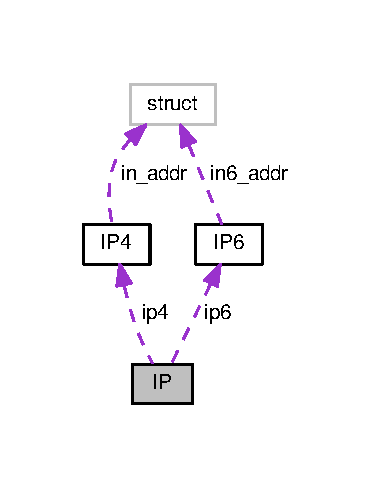
\includegraphics[width=178pt]{db/d49/struct_i_p__coll__graph}
\end{center}
\end{figure}
\subsection*{Data Fields}
\begin{DoxyCompactItemize}
\item 
uint8\+\_\+t \hyperlink{struct_i_p_adad4493a852deb413bb8c515368deaac}{family}
\item 
\begin{tabbing}
xx\=xx\=xx\=xx\=xx\=xx\=xx\=xx\=xx\=\kill
union \{\\
\>\hyperlink{union_i_p4}{IP4} \hyperlink{struct_i_p_aca19646000f55aa927406e68fc41ecf9}{ip4}\\
\>\hyperlink{union_i_p6}{IP6} \hyperlink{struct_i_p_a14c606eb5ffb078c38ad854dc4e79507}{ip6}\\
\}; \\

\end{tabbing}\end{DoxyCompactItemize}


\subsection{Detailed Description}


Definition at line 153 of file network.\+h.



\subsection{Field Documentation}
\hypertarget{struct_i_p_acd63477cf058774f4a8446acedfc9aff}{\subsubsection[{"@23}]{\setlength{\rightskip}{0pt plus 5cm}union \{ ... \} }}\label{struct_i_p_acd63477cf058774f4a8446acedfc9aff}
\hypertarget{struct_i_p_adad4493a852deb413bb8c515368deaac}{\index{I\+P@{I\+P}!family@{family}}
\index{family@{family}!I\+P@{I\+P}}
\subsubsection[{family}]{\setlength{\rightskip}{0pt plus 5cm}uint8\+\_\+t family}}\label{struct_i_p_adad4493a852deb413bb8c515368deaac}


Definition at line 154 of file network.\+h.



Referenced by add\+\_\+tcp\+\_\+relay\+\_\+instance(), addr\+\_\+parse\+\_\+ip(), addr\+\_\+resolve(), addto\+\_\+lists(), broadcast\+\_\+ip(), candidates\+\_\+create\+\_\+new(), candidates\+\_\+update\+\_\+assoc(), client\+\_\+or\+\_\+ip\+\_\+port\+\_\+in\+\_\+list(), connect\+\_\+sock\+\_\+to(), connect\+\_\+to\+\_\+saved\+\_\+tcp\+\_\+relays(), crypto\+\_\+connection\+\_\+add\+\_\+source(), D\+H\+T\+\_\+bootstrap\+\_\+from\+\_\+address(), do\+\_\+friend\+\_\+connections(), do\+\_\+messenger(), entry\+\_\+assoc(), entry\+\_\+heard\+\_\+get(), entry\+\_\+heard\+\_\+store(), friend\+\_\+add\+\_\+tcp\+\_\+relay(), handle\+\_\+dhtpk\+\_\+announce(), handle\+\_\+new\+\_\+connections(), handle\+\_\+recv\+\_\+1(), handle\+\_\+tcp\+\_\+onion(), handle\+\_\+\+T\+C\+P\+\_\+packet(), in\+\_\+list(), ip\+\_\+equal(), ip\+\_\+init(), ip\+\_\+isset(), ip\+\_\+ntoa(), ip\+\_\+pack(), ip\+\_\+parse\+\_\+addr(), ip\+\_\+unpack(), L\+A\+N\+\_\+ip(), Local\+\_\+ip(), main(), new\+\_\+networking\+\_\+ex(), new\+\_\+\+T\+C\+P\+\_\+connection(), onion\+\_\+add\+\_\+bs\+\_\+path\+\_\+node(), onion\+\_\+add\+\_\+path\+\_\+node(), proxy\+\_\+socks5\+\_\+generate\+\_\+connection\+\_\+request(), proxy\+\_\+socks5\+\_\+read\+\_\+connection\+\_\+response(), random\+\_\+nodes\+\_\+path\+\_\+onion(), receivepacket(), replace\+\_\+all(), returnedip\+\_\+ports(), send\+\_\+onion\+\_\+packet\+\_\+tcp\+\_\+udp(), send\+\_\+packet\+\_\+to(), sendpacket(), set\+\_\+direct\+\_\+ip\+\_\+port(), S\+T\+A\+R\+T\+\_\+\+T\+E\+S\+T(), tcp\+\_\+copy\+\_\+connected\+\_\+relays(), tcp\+\_\+oob\+\_\+callback(), test\+\_\+addto\+\_\+lists\+\_\+bad(), test\+\_\+addto\+\_\+lists\+\_\+good(), test\+\_\+addto\+\_\+lists\+\_\+possible\+\_\+bad(), test\+\_\+addto\+\_\+lists\+\_\+update(), to\+\_\+host\+\_\+family(), to\+\_\+net\+\_\+family(), tox\+\_\+add\+\_\+tcp\+\_\+relay(), tox\+\_\+bootstrap(), tox\+\_\+new(), and unpack\+\_\+nodes().

\hypertarget{struct_i_p_aca19646000f55aa927406e68fc41ecf9}{\index{I\+P@{I\+P}!ip4@{ip4}}
\index{ip4@{ip4}!I\+P@{I\+P}}
\subsubsection[{ip4}]{\setlength{\rightskip}{0pt plus 5cm}{\bf I\+P4} ip4}}\label{struct_i_p_aca19646000f55aa927406e68fc41ecf9}


Definition at line 156 of file network.\+h.



Referenced by addr\+\_\+parse\+\_\+ip(), addr\+\_\+resolve(), addto\+\_\+lists(), broadcast\+\_\+ip(), connect\+\_\+sock\+\_\+to(), do\+\_\+messenger(), ip\+\_\+equal(), ip\+\_\+ntoa(), ip\+\_\+pack(), ip\+\_\+parse\+\_\+addr(), ip\+\_\+unpack(), L\+A\+N\+\_\+ip(), Local\+\_\+ip(), main(), new\+\_\+networking\+\_\+ex(), proxy\+\_\+socks5\+\_\+generate\+\_\+connection\+\_\+request(), random\+\_\+nodes\+\_\+path\+\_\+onion(), receivepacket(), returnedip\+\_\+ports(), send\+\_\+onion\+\_\+packet\+\_\+tcp\+\_\+udp(), sendpacket(), S\+T\+A\+R\+T\+\_\+\+T\+E\+S\+T(), tox\+\_\+add\+\_\+tcp\+\_\+relay(), and tox\+\_\+bootstrap().

\hypertarget{struct_i_p_a14c606eb5ffb078c38ad854dc4e79507}{\index{I\+P@{I\+P}!ip6@{ip6}}
\index{ip6@{ip6}!I\+P@{I\+P}}
\subsubsection[{ip6}]{\setlength{\rightskip}{0pt plus 5cm}{\bf I\+P6} ip6}}\label{struct_i_p_a14c606eb5ffb078c38ad854dc4e79507}


Definition at line 157 of file network.\+h.



Referenced by addr\+\_\+parse\+\_\+ip(), addr\+\_\+resolve(), addto\+\_\+lists(), broadcast\+\_\+ip(), connect\+\_\+sock\+\_\+to(), crypto\+\_\+connection\+\_\+add\+\_\+source(), handle\+\_\+onion\+\_\+recv\+\_\+1(), handle\+\_\+\+T\+C\+P\+\_\+packet(), ip\+\_\+equal(), ip\+\_\+ntoa(), ip\+\_\+pack(), ip\+\_\+parse\+\_\+addr(), ip\+\_\+unpack(), L\+A\+N\+\_\+ip(), Local\+\_\+ip(), new\+\_\+networking\+\_\+ex(), new\+\_\+onions(), proxy\+\_\+socks5\+\_\+generate\+\_\+connection\+\_\+request(), receivepacket(), returnedip\+\_\+ports(), sendpacket(), S\+T\+A\+R\+T\+\_\+\+T\+E\+S\+T(), tcp\+\_\+oob\+\_\+callback(), tox\+\_\+add\+\_\+tcp\+\_\+relay(), and tox\+\_\+bootstrap().



The documentation for this struct was generated from the following file\+:\begin{DoxyCompactItemize}
\item 
toxcore/\hyperlink{network_8h}{network.\+h}\end{DoxyCompactItemize}

\hypertarget{union_i_p4}{\section{I\+P4 Union Reference}
\label{union_i_p4}\index{I\+P4@{I\+P4}}
}


Collaboration diagram for I\+P4\+:
\nopagebreak
\begin{figure}[H]
\begin{center}
\leavevmode
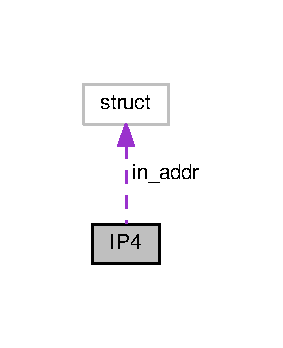
\includegraphics[width=136pt]{union_i_p4__coll__graph}
\end{center}
\end{figure}
\subsection*{Data Fields}
\begin{DoxyCompactItemize}
\item 
\hypertarget{union_i_p4_a73b9a57544f1edd6e2187aca636c75ef}{uint8\+\_\+t {\bfseries uint8} \mbox{[}4\mbox{]}}\label{union_i_p4_a73b9a57544f1edd6e2187aca636c75ef}

\item 
\hypertarget{union_i_p4_ac29b55876c4db8c2e69e138039fb7a8a}{uint16\+\_\+t {\bfseries uint16} \mbox{[}2\mbox{]}}\label{union_i_p4_ac29b55876c4db8c2e69e138039fb7a8a}

\item 
\hypertarget{union_i_p4_a5ad776be1fb768f3399aafcd1b58b3a2}{uint32\+\_\+t {\bfseries uint32}}\label{union_i_p4_a5ad776be1fb768f3399aafcd1b58b3a2}

\item 
\hypertarget{union_i_p4_a5a47f63dce37e6eb6be40f022434b1c5}{struct in\+\_\+addr {\bfseries in\+\_\+addr}}\label{union_i_p4_a5a47f63dce37e6eb6be40f022434b1c5}

\end{DoxyCompactItemize}


\subsection{Detailed Description}


Definition at line 136 of file network.\+h.



The documentation for this union was generated from the following file\+:\begin{DoxyCompactItemize}
\item 
toxcore/network.\+h\end{DoxyCompactItemize}

\hypertarget{union_i_p6}{\section{I\+P6 Union Reference}
\label{union_i_p6}\index{I\+P6@{I\+P6}}
}


Collaboration diagram for I\+P6\+:\nopagebreak
\begin{figure}[H]
\begin{center}
\leavevmode
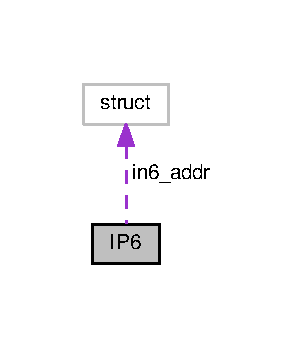
\includegraphics[width=141pt]{union_i_p6__coll__graph}
\end{center}
\end{figure}
\subsection*{Data Fields}
\begin{DoxyCompactItemize}
\item 
\hypertarget{union_i_p6_a6b067d428eefbf1754aa09429b1ba524}{uint8\+\_\+t {\bfseries uint8} \mbox{[}16\mbox{]}}\label{union_i_p6_a6b067d428eefbf1754aa09429b1ba524}

\item 
\hypertarget{union_i_p6_af0f89d2fc8c3ccbcc4fca0156563fcfe}{uint16\+\_\+t {\bfseries uint16} \mbox{[}8\mbox{]}}\label{union_i_p6_af0f89d2fc8c3ccbcc4fca0156563fcfe}

\item 
\hypertarget{union_i_p6_a1d8ab1f6c1da5565bed41e7095610dea}{uint32\+\_\+t {\bfseries uint32} \mbox{[}4\mbox{]}}\label{union_i_p6_a1d8ab1f6c1da5565bed41e7095610dea}

\item 
\hypertarget{union_i_p6_a36c7a85cc2c5062edd5ebf13d46fa343}{uint64\+\_\+t {\bfseries uint64} \mbox{[}2\mbox{]}}\label{union_i_p6_a36c7a85cc2c5062edd5ebf13d46fa343}

\item 
\hypertarget{union_i_p6_ac312c20ade57f180c50585e9ea42314c}{struct in6\+\_\+addr {\bfseries in6\+\_\+addr}}\label{union_i_p6_ac312c20ade57f180c50585e9ea42314c}

\end{DoxyCompactItemize}


\subsection{Detailed Description}


Definition at line 144 of file network.\+h.



The documentation for this union was generated from the following file\+:\begin{DoxyCompactItemize}
\item 
toxcore/network.\+h\end{DoxyCompactItemize}

\hypertarget{struct_i_p___port}{\section{I\+P\+\_\+\+Port Struct Reference}
\label{struct_i_p___port}\index{I\+P\+\_\+\+Port@{I\+P\+\_\+\+Port}}
}


{\ttfamily \#include $<$network.\+h$>$}



Collaboration diagram for I\+P\+\_\+\+Port\+:
\nopagebreak
\begin{figure}[H]
\begin{center}
\leavevmode
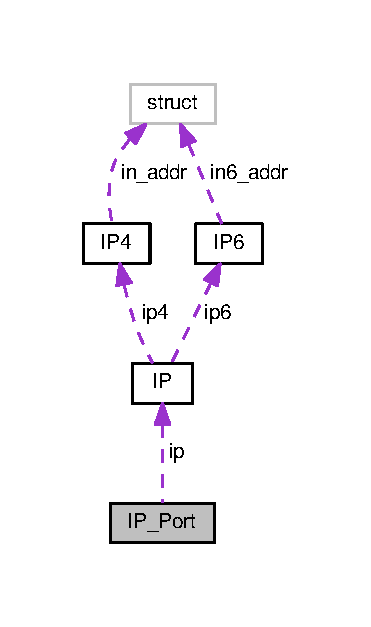
\includegraphics[width=178pt]{d0/de8/struct_i_p___port__coll__graph}
\end{center}
\end{figure}
\subsection*{Data Fields}
\begin{DoxyCompactItemize}
\item 
\hyperlink{struct_i_p}{I\+P} \hyperlink{struct_i_p___port_a0c6193a337a223c63411b2fe722d79ec}{ip}
\item 
uint16\+\_\+t \hyperlink{struct_i_p___port_a8e0798404bf2cf5dabb84c5ba9a4f236}{port}
\end{DoxyCompactItemize}


\subsection{Detailed Description}


Definition at line 162 of file network.\+h.



\subsection{Field Documentation}
\hypertarget{struct_i_p___port_a0c6193a337a223c63411b2fe722d79ec}{\index{I\+P\+\_\+\+Port@{I\+P\+\_\+\+Port}!ip@{ip}}
\index{ip@{ip}!I\+P\+\_\+\+Port@{I\+P\+\_\+\+Port}}
\subsubsection[{ip}]{\setlength{\rightskip}{0pt plus 5cm}{\bf I\+P} ip}}\label{struct_i_p___port_a0c6193a337a223c63411b2fe722d79ec}


Definition at line 163 of file network.\+h.



Referenced by add\+\_\+tcp\+\_\+relay\+\_\+instance(), add\+\_\+to\+\_\+ping(), addto\+\_\+lists(), Assoc\+\_\+get\+\_\+close\+\_\+entries(), candidates\+\_\+create\+\_\+new(), candidates\+\_\+update\+\_\+assoc(), client\+\_\+or\+\_\+ip\+\_\+port\+\_\+in\+\_\+list(), client\+\_\+ping\+\_\+nodes(), connect\+\_\+sock\+\_\+to(), connect\+\_\+to\+\_\+saved\+\_\+tcp\+\_\+relays(), crypto\+\_\+connection\+\_\+add\+\_\+source(), D\+H\+T\+\_\+bootstrap\+\_\+from\+\_\+address(), D\+H\+T\+\_\+getfriendip(), D\+H\+T\+\_\+non\+\_\+lan\+\_\+connected(), do\+\_\+\+Assoc(), do\+\_\+friend\+\_\+connections(), do\+\_\+messenger(), do\+\_\+to\+\_\+ping(), entry\+\_\+assoc(), entry\+\_\+heard\+\_\+get(), entry\+\_\+heard\+\_\+store(), friend\+\_\+add\+\_\+tcp\+\_\+relay(), friend\+\_\+iplist(), get\+\_\+close\+\_\+nodes\+\_\+inner(), handle\+\_\+announce\+\_\+request(), handle\+\_\+dhtpk\+\_\+announce(), handle\+\_\+\+L\+A\+Ndiscovery(), handle\+\_\+new\+\_\+connections(), handle\+\_\+onion\+\_\+recv\+\_\+1(), handle\+\_\+recv\+\_\+1(), handle\+\_\+tcp\+\_\+onion(), handle\+\_\+\+T\+C\+P\+\_\+packet(), in\+\_\+list(), ipport\+\_\+equal(), ipport\+\_\+isset(), ipport\+\_\+pack(), ipport\+\_\+unpack(), N\+A\+T\+\_\+commonip(), new\+\_\+\+T\+C\+P\+\_\+connection(), onion\+\_\+add\+\_\+bs\+\_\+path\+\_\+node(), onion\+\_\+add\+\_\+path\+\_\+node(), print\+\_\+assoc(), print\+\_\+friendlist(), proxy\+\_\+http\+\_\+generate\+\_\+connection\+\_\+request(), proxy\+\_\+socks5\+\_\+generate\+\_\+connection\+\_\+request(), proxy\+\_\+socks5\+\_\+read\+\_\+connection\+\_\+response(), punch\+\_\+holes(), random\+\_\+nodes\+\_\+path\+\_\+onion(), receivepacket(), replace\+\_\+all(), returnedip\+\_\+ports(), route\+\_\+packet(), route\+\_\+tofriend(), routeone\+\_\+tofriend(), send\+\_\+hardening\+\_\+getnode\+\_\+res(), send\+\_\+\+L\+A\+Ndiscovery(), send\+\_\+onion\+\_\+packet\+\_\+tcp\+\_\+udp(), send\+\_\+packet\+\_\+to(), sendnodes\+\_\+ipv6(), sendpacket(), set\+\_\+direct\+\_\+ip\+\_\+port(), S\+T\+A\+R\+T\+\_\+\+T\+E\+S\+T(), tcp\+\_\+copy\+\_\+connected\+\_\+relays(), tcp\+\_\+oob\+\_\+callback(), test\+\_\+addto\+\_\+lists(), test\+\_\+addto\+\_\+lists\+\_\+bad(), test\+\_\+addto\+\_\+lists\+\_\+good(), test\+\_\+addto\+\_\+lists\+\_\+possible\+\_\+bad(), test\+\_\+addto\+\_\+lists\+\_\+update(), tox\+\_\+add\+\_\+tcp\+\_\+relay(), tox\+\_\+bootstrap(), tox\+\_\+new(), and unpack\+\_\+nodes().

\hypertarget{struct_i_p___port_a8e0798404bf2cf5dabb84c5ba9a4f236}{\index{I\+P\+\_\+\+Port@{I\+P\+\_\+\+Port}!port@{port}}
\index{port@{port}!I\+P\+\_\+\+Port@{I\+P\+\_\+\+Port}}
\subsubsection[{port}]{\setlength{\rightskip}{0pt plus 5cm}uint16\+\_\+t port}}\label{struct_i_p___port_a8e0798404bf2cf5dabb84c5ba9a4f236}


Definition at line 164 of file network.\+h.



Referenced by connect\+\_\+sock\+\_\+to(), D\+H\+T\+\_\+bootstrap\+\_\+from\+\_\+address(), D\+H\+T\+\_\+getfriendip(), do\+\_\+\+Assoc(), do\+\_\+messenger(), handle\+\_\+\+T\+C\+P\+\_\+packet(), ipport\+\_\+equal(), ipport\+\_\+isset(), ipport\+\_\+pack(), ipport\+\_\+unpack(), print\+\_\+assoc(), print\+\_\+friendlist(), proxy\+\_\+http\+\_\+generate\+\_\+connection\+\_\+request(), proxy\+\_\+socks5\+\_\+generate\+\_\+connection\+\_\+request(), punch\+\_\+holes(), receivepacket(), replace\+\_\+all(), send\+\_\+\+L\+A\+Ndiscovery(), sendpacket(), S\+T\+A\+R\+T\+\_\+\+T\+E\+S\+T(), tcp\+\_\+oob\+\_\+callback(), test\+\_\+addto\+\_\+lists(), test\+\_\+addto\+\_\+lists\+\_\+bad(), test\+\_\+addto\+\_\+lists\+\_\+good(), test\+\_\+addto\+\_\+lists\+\_\+possible\+\_\+bad(), test\+\_\+addto\+\_\+lists\+\_\+update(), tox\+\_\+add\+\_\+tcp\+\_\+relay(), tox\+\_\+bootstrap(), and tox\+\_\+new().



The documentation for this struct was generated from the following file\+:\begin{DoxyCompactItemize}
\item 
toxcore/\hyperlink{network_8h}{network.\+h}\end{DoxyCompactItemize}

\hypertarget{struct_i_p_p_ts}{\section{I\+P\+P\+Ts Struct Reference}
\label{struct_i_p_p_ts}\index{I\+P\+P\+Ts@{I\+P\+P\+Ts}}
}


Collaboration diagram for I\+P\+P\+Ts\+:\nopagebreak
\begin{figure}[H]
\begin{center}
\leavevmode
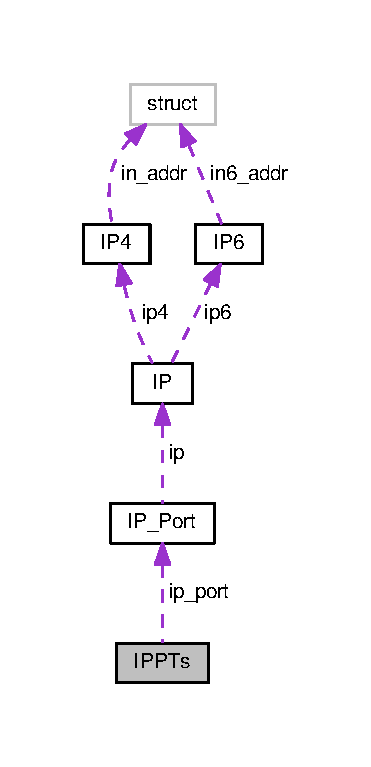
\includegraphics[width=178pt]{struct_i_p_p_ts__coll__graph}
\end{center}
\end{figure}
\subsection*{Data Fields}
\begin{DoxyCompactItemize}
\item 
\hypertarget{struct_i_p_p_ts_a86e2a5a56c0dd22df6e8b8a10e40f9e4}{\hyperlink{struct_i_p___port}{I\+P\+\_\+\+Port} {\bfseries ip\+\_\+port}}\label{struct_i_p_p_ts_a86e2a5a56c0dd22df6e8b8a10e40f9e4}

\item 
\hypertarget{struct_i_p_p_ts_a465bef81f6478756e5443025b1f2ddfa}{uint64\+\_\+t {\bfseries timestamp}}\label{struct_i_p_p_ts_a465bef81f6478756e5443025b1f2ddfa}

\end{DoxyCompactItemize}


\subsection{Detailed Description}


Definition at line 69 of file D\+H\+T.\+h.



The documentation for this struct was generated from the following file\+:\begin{DoxyCompactItemize}
\item 
toxcore/D\+H\+T.\+h\end{DoxyCompactItemize}

\hypertarget{struct_i_p_p_ts_png}{\section{I\+P\+P\+Ts\+Png Struct Reference}
\label{struct_i_p_p_ts_png}\index{I\+P\+P\+Ts\+Png@{I\+P\+P\+Ts\+Png}}
}


Collaboration diagram for I\+P\+P\+Ts\+Png\+:
\nopagebreak
\begin{figure}[H]
\begin{center}
\leavevmode
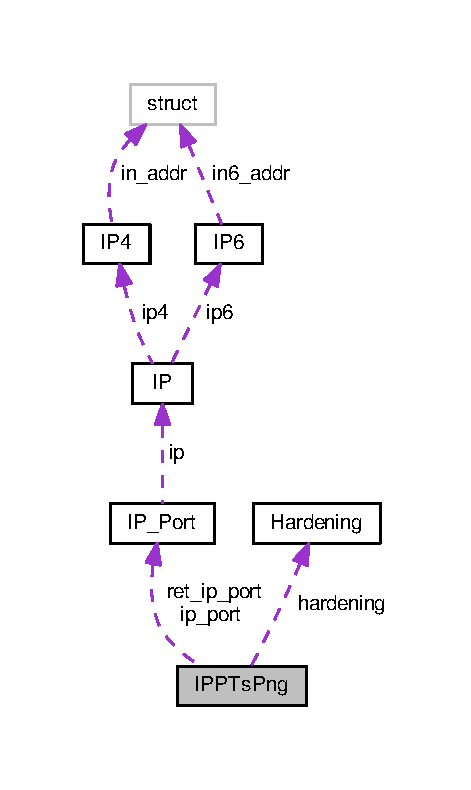
\includegraphics[width=226pt]{struct_i_p_p_ts_png__coll__graph}
\end{center}
\end{figure}
\subsection*{Data Fields}
\begin{DoxyCompactItemize}
\item 
\hypertarget{struct_i_p_p_ts_png_a86e2a5a56c0dd22df6e8b8a10e40f9e4}{\hyperlink{struct_i_p___port}{I\+P\+\_\+\+Port} {\bfseries ip\+\_\+port}}\label{struct_i_p_p_ts_png_a86e2a5a56c0dd22df6e8b8a10e40f9e4}

\item 
\hypertarget{struct_i_p_p_ts_png_a465bef81f6478756e5443025b1f2ddfa}{uint64\+\_\+t {\bfseries timestamp}}\label{struct_i_p_p_ts_png_a465bef81f6478756e5443025b1f2ddfa}

\item 
\hypertarget{struct_i_p_p_ts_png_a4049204f6c392628d31be6c39f03e031}{uint64\+\_\+t {\bfseries last\+\_\+pinged}}\label{struct_i_p_p_ts_png_a4049204f6c392628d31be6c39f03e031}

\item 
\hypertarget{struct_i_p_p_ts_png_a247a5bc6669d45b7241b58223ce8fd1d}{\hyperlink{struct_hardening}{Hardening} {\bfseries hardening}}\label{struct_i_p_p_ts_png_a247a5bc6669d45b7241b58223ce8fd1d}

\item 
\hypertarget{struct_i_p_p_ts_png_a28f2dcc657352ee4855d05ed42e4a4af}{\hyperlink{struct_i_p___port}{I\+P\+\_\+\+Port} {\bfseries ret\+\_\+ip\+\_\+port}}\label{struct_i_p_p_ts_png_a28f2dcc657352ee4855d05ed42e4a4af}

\item 
\hypertarget{struct_i_p_p_ts_png_a5a40b83400feebb632862f593ad5e4a7}{uint64\+\_\+t {\bfseries ret\+\_\+timestamp}}\label{struct_i_p_p_ts_png_a5a40b83400feebb632862f593ad5e4a7}

\end{DoxyCompactItemize}


\subsection{Detailed Description}


Definition at line 95 of file D\+H\+T.\+h.



The documentation for this struct was generated from the following file\+:\begin{DoxyCompactItemize}
\item 
toxcore/D\+H\+T.\+h\end{DoxyCompactItemize}

\hypertarget{struct_last___pinged}{\section{Last\+\_\+\+Pinged Struct Reference}
\label{struct_last___pinged}\index{Last\+\_\+\+Pinged@{Last\+\_\+\+Pinged}}
}
\subsection*{Data Fields}
\begin{DoxyCompactItemize}
\item 
\hypertarget{struct_last___pinged_aaa806bb1136fb3d4b5d8d8970b596ff7}{uint8\+\_\+t {\bfseries public\+\_\+key} \mbox{[}crypto\+\_\+box\+\_\+\+P\+U\+B\+L\+I\+C\+K\+E\+Y\+B\+Y\+T\+E\+S\mbox{]}}\label{struct_last___pinged_aaa806bb1136fb3d4b5d8d8970b596ff7}

\item 
\hypertarget{struct_last___pinged_a465bef81f6478756e5443025b1f2ddfa}{uint64\+\_\+t {\bfseries timestamp}}\label{struct_last___pinged_a465bef81f6478756e5443025b1f2ddfa}

\end{DoxyCompactItemize}


\subsection{Detailed Description}


Definition at line 85 of file onion\+\_\+client.\+h.



The documentation for this struct was generated from the following file\+:\begin{DoxyCompactItemize}
\item 
toxcore/onion\+\_\+client.\+h\end{DoxyCompactItemize}

\hypertarget{structlogger}{\section{logger Struct Reference}
\label{structlogger}\index{logger@{logger}}
}
\subsection*{Data Fields}
\begin{DoxyCompactItemize}
\item 
F\+I\+L\+E $\ast$ \hyperlink{structlogger_ab936051f5aaca44c6c3c41dee0d19c36}{log\+\_\+file}
\item 
\hyperlink{logger_8h_aa5a9053636a30269210c54e734e0d583}{L\+O\+G\+\_\+\+L\+E\+V\+E\+L} \hyperlink{structlogger_a77f7159081bd39a76d8b86af56256201}{level}
\item 
uint64\+\_\+t \hyperlink{structlogger_a5b11efea935978e9f1913e964a5e5396}{start\+\_\+time}
\item 
char $\ast$ \hyperlink{structlogger_aecb3b0d045ada529257a2fbf8f829599}{id}
\item 
char $\ast$ \hyperlink{structlogger_a756188d61db4922010ba1bf67c2f381e}{tstr}
\item 
char $\ast$ \hyperlink{structlogger_a56126aabcbc86b3b9b826e08036685eb}{posstr}
\item 
char $\ast$ \hyperlink{structlogger_a32d2f5216cddb59c7cc8fb2806a7e727}{msg}
\item 
pthread\+\_\+mutex\+\_\+t \hyperlink{structlogger_ab4293016252c4d4e63549b0773fa0f33}{mutex} \mbox{[}1\mbox{]}
\end{DoxyCompactItemize}


\subsection{Detailed Description}


Definition at line 47 of file logger.\+c.



\subsection{Field Documentation}
\hypertarget{structlogger_aecb3b0d045ada529257a2fbf8f829599}{\index{logger@{logger}!id@{id}}
\index{id@{id}!logger@{logger}}
\subsubsection[{id}]{\setlength{\rightskip}{0pt plus 5cm}char$\ast$ id}}\label{structlogger_aecb3b0d045ada529257a2fbf8f829599}


Definition at line 51 of file logger.\+c.



Referenced by logger\+\_\+kill(), logger\+\_\+new(), and logger\+\_\+write().

\hypertarget{structlogger_a77f7159081bd39a76d8b86af56256201}{\index{logger@{logger}!level@{level}}
\index{level@{level}!logger@{logger}}
\subsubsection[{level}]{\setlength{\rightskip}{0pt plus 5cm}{\bf L\+O\+G\+\_\+\+L\+E\+V\+E\+L} level}}\label{structlogger_a77f7159081bd39a76d8b86af56256201}


Definition at line 49 of file logger.\+c.



Referenced by logger\+\_\+new(), and logger\+\_\+write().

\hypertarget{structlogger_ab936051f5aaca44c6c3c41dee0d19c36}{\index{logger@{logger}!log\+\_\+file@{log\+\_\+file}}
\index{log\+\_\+file@{log\+\_\+file}!logger@{logger}}
\subsubsection[{log\+\_\+file}]{\setlength{\rightskip}{0pt plus 5cm}F\+I\+L\+E$\ast$ log\+\_\+file}}\label{structlogger_ab936051f5aaca44c6c3c41dee0d19c36}


Definition at line 48 of file logger.\+c.



Referenced by logger\+\_\+kill(), logger\+\_\+new(), and logger\+\_\+write().

\hypertarget{structlogger_a32d2f5216cddb59c7cc8fb2806a7e727}{\index{logger@{logger}!msg@{msg}}
\index{msg@{msg}!logger@{logger}}
\subsubsection[{msg}]{\setlength{\rightskip}{0pt plus 5cm}char$\ast$ msg}}\label{structlogger_a32d2f5216cddb59c7cc8fb2806a7e727}


Definition at line 56 of file logger.\+c.



Referenced by logger\+\_\+kill(), logger\+\_\+new(), and logger\+\_\+write().

\hypertarget{structlogger_ab4293016252c4d4e63549b0773fa0f33}{\index{logger@{logger}!mutex@{mutex}}
\index{mutex@{mutex}!logger@{logger}}
\subsubsection[{mutex}]{\setlength{\rightskip}{0pt plus 5cm}pthread\+\_\+mutex\+\_\+t mutex\mbox{[}1\mbox{]}}}\label{structlogger_ab4293016252c4d4e63549b0773fa0f33}


Definition at line 59 of file logger.\+c.



Referenced by logger\+\_\+kill(), logger\+\_\+new(), and logger\+\_\+write().

\hypertarget{structlogger_a56126aabcbc86b3b9b826e08036685eb}{\index{logger@{logger}!posstr@{posstr}}
\index{posstr@{posstr}!logger@{logger}}
\subsubsection[{posstr}]{\setlength{\rightskip}{0pt plus 5cm}char$\ast$ posstr}}\label{structlogger_a56126aabcbc86b3b9b826e08036685eb}


Definition at line 55 of file logger.\+c.



Referenced by logger\+\_\+kill(), logger\+\_\+new(), and logger\+\_\+write().

\hypertarget{structlogger_a5b11efea935978e9f1913e964a5e5396}{\index{logger@{logger}!start\+\_\+time@{start\+\_\+time}}
\index{start\+\_\+time@{start\+\_\+time}!logger@{logger}}
\subsubsection[{start\+\_\+time}]{\setlength{\rightskip}{0pt plus 5cm}uint64\+\_\+t start\+\_\+time}}\label{structlogger_a5b11efea935978e9f1913e964a5e5396}


Definition at line 50 of file logger.\+c.



Referenced by logger\+\_\+new().

\hypertarget{structlogger_a756188d61db4922010ba1bf67c2f381e}{\index{logger@{logger}!tstr@{tstr}}
\index{tstr@{tstr}!logger@{logger}}
\subsubsection[{tstr}]{\setlength{\rightskip}{0pt plus 5cm}char$\ast$ tstr}}\label{structlogger_a756188d61db4922010ba1bf67c2f381e}


Definition at line 54 of file logger.\+c.



Referenced by logger\+\_\+kill(), logger\+\_\+new(), and logger\+\_\+write().



The documentation for this struct was generated from the following file\+:\begin{DoxyCompactItemize}
\item 
toxcore/\hyperlink{logger_8c}{logger.\+c}\end{DoxyCompactItemize}

\hypertarget{struct_messenger}{\section{Messenger Struct Reference}
\label{struct_messenger}\index{Messenger@{Messenger}}
}


Collaboration diagram for Messenger\+:\nopagebreak
\begin{figure}[H]
\begin{center}
\leavevmode
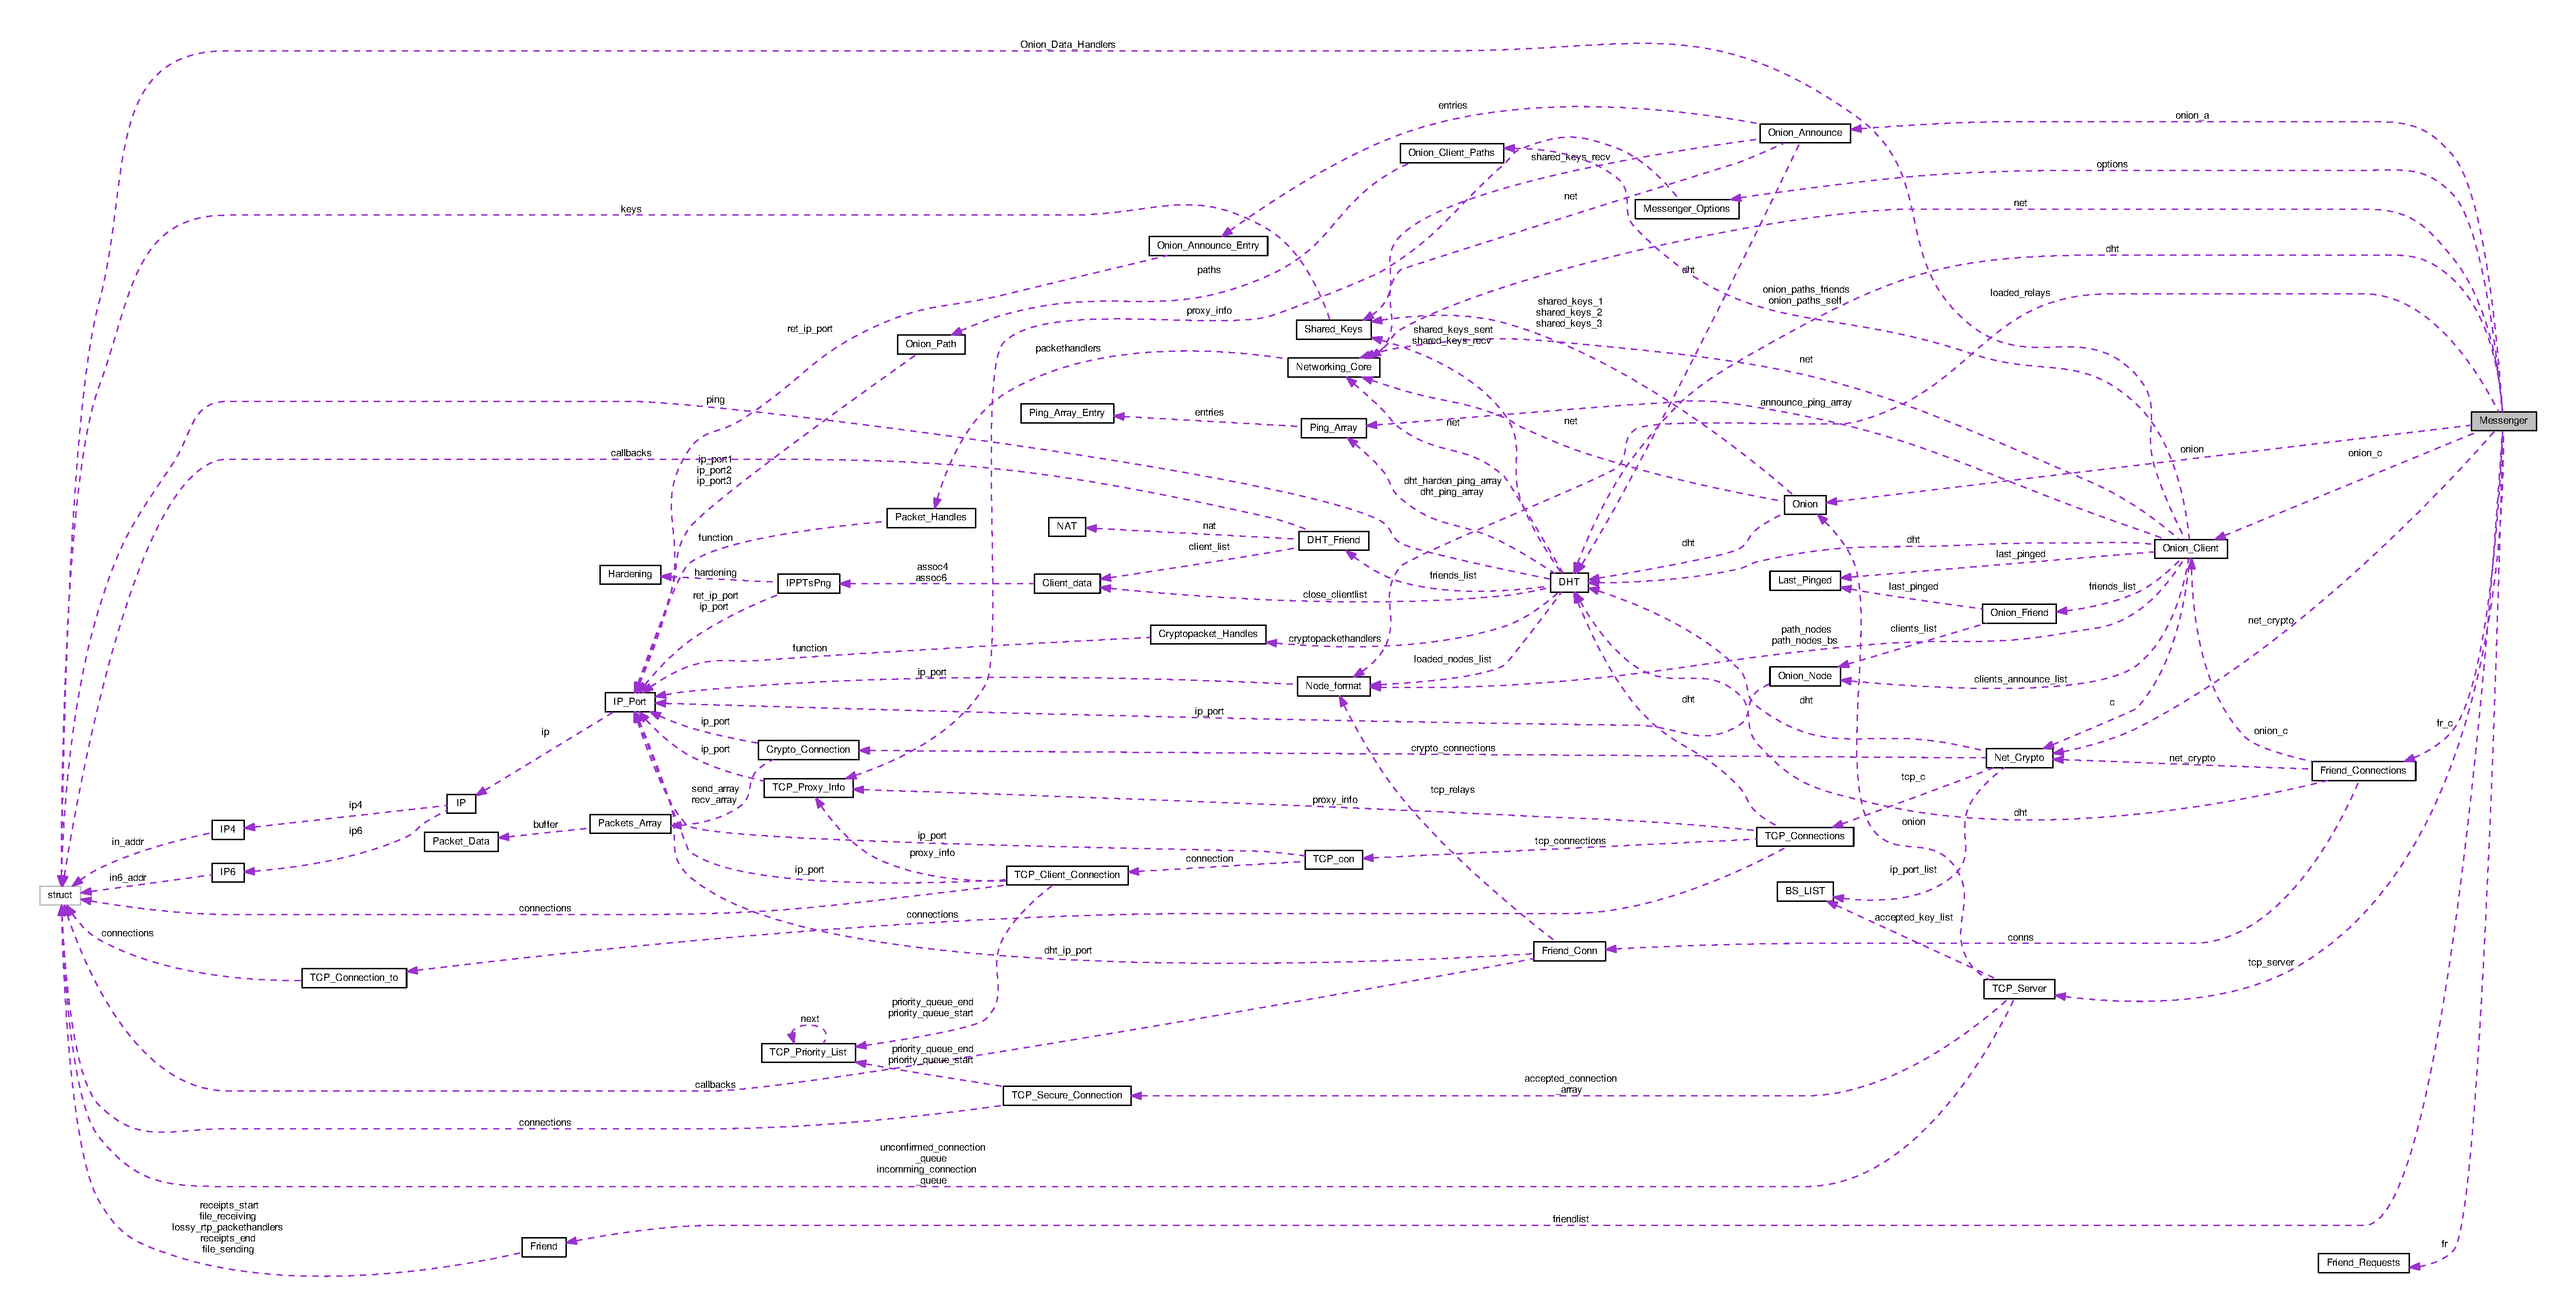
\includegraphics[width=350pt]{struct_messenger__coll__graph}
\end{center}
\end{figure}
\subsection*{Data Fields}
\begin{DoxyCompactItemize}
\item 
\hypertarget{struct_messenger_aa14ea2f67950f57fe4235d7375a2216c}{\hyperlink{struct_networking___core}{Networking\+\_\+\+Core} $\ast$ {\bfseries net}}\label{struct_messenger_aa14ea2f67950f57fe4235d7375a2216c}

\item 
\hypertarget{struct_messenger_ab06a41217a1e9b5985555e19e088ae94}{\hyperlink{struct_net___crypto}{Net\+\_\+\+Crypto} $\ast$ {\bfseries net\+\_\+crypto}}\label{struct_messenger_ab06a41217a1e9b5985555e19e088ae94}

\item 
\hypertarget{struct_messenger_a8b3d6ce8745acc52695e252bdb1531b6}{\hyperlink{struct_d_h_t}{D\+H\+T} $\ast$ {\bfseries dht}}\label{struct_messenger_a8b3d6ce8745acc52695e252bdb1531b6}

\item 
\hypertarget{struct_messenger_a66fb4bf67c711a5ed3e7bbecec7fde30}{\hyperlink{struct_onion}{Onion} $\ast$ {\bfseries onion}}\label{struct_messenger_a66fb4bf67c711a5ed3e7bbecec7fde30}

\item 
\hypertarget{struct_messenger_a3a345721fb6be385f4b4519679a4609f}{\hyperlink{struct_onion___announce}{Onion\+\_\+\+Announce} $\ast$ {\bfseries onion\+\_\+a}}\label{struct_messenger_a3a345721fb6be385f4b4519679a4609f}

\item 
\hypertarget{struct_messenger_ae202b81f9a2c2fa80fd310a0996795fc}{\hyperlink{struct_onion___client}{Onion\+\_\+\+Client} $\ast$ {\bfseries onion\+\_\+c}}\label{struct_messenger_ae202b81f9a2c2fa80fd310a0996795fc}

\item 
\hypertarget{struct_messenger_ae26eb43a606fff20fe70209d051c40f9}{\hyperlink{struct_friend___connections}{Friend\+\_\+\+Connections} $\ast$ {\bfseries fr\+\_\+c}}\label{struct_messenger_ae26eb43a606fff20fe70209d051c40f9}

\item 
\hypertarget{struct_messenger_afc53e878009e340983270593e62cadef}{\hyperlink{struct_t_c_p___server}{T\+C\+P\+\_\+\+Server} $\ast$ {\bfseries tcp\+\_\+server}}\label{struct_messenger_afc53e878009e340983270593e62cadef}

\item 
\hypertarget{struct_messenger_ae46787dbb8f8dce47f8fdc6192cf788d}{\hyperlink{struct_friend___requests}{Friend\+\_\+\+Requests} {\bfseries fr}}\label{struct_messenger_ae46787dbb8f8dce47f8fdc6192cf788d}

\item 
\hypertarget{struct_messenger_a11b8cc6595eea79e65c978209278e683}{uint8\+\_\+t {\bfseries name} \mbox{[}M\+A\+X\+\_\+\+N\+A\+M\+E\+\_\+\+L\+E\+N\+G\+T\+H\mbox{]}}\label{struct_messenger_a11b8cc6595eea79e65c978209278e683}

\item 
\hypertarget{struct_messenger_a3573d7a906b26e9999cd74f2c4066601}{uint16\+\_\+t {\bfseries name\+\_\+length}}\label{struct_messenger_a3573d7a906b26e9999cd74f2c4066601}

\item 
\hypertarget{struct_messenger_a8f12612ac1191135a1a5b1cbcbc82852}{uint8\+\_\+t {\bfseries statusmessage} \mbox{[}M\+A\+X\+\_\+\+S\+T\+A\+T\+U\+S\+M\+E\+S\+S\+A\+G\+E\+\_\+\+L\+E\+N\+G\+T\+H\mbox{]}}\label{struct_messenger_a8f12612ac1191135a1a5b1cbcbc82852}

\item 
\hypertarget{struct_messenger_a43fe9dde52dc12e90933150eca91c0c3}{uint16\+\_\+t {\bfseries statusmessage\+\_\+length}}\label{struct_messenger_a43fe9dde52dc12e90933150eca91c0c3}

\item 
\hypertarget{struct_messenger_adde524f5a15465585cbc2543cd0b2710}{U\+S\+E\+R\+S\+T\+A\+T\+U\+S {\bfseries userstatus}}\label{struct_messenger_adde524f5a15465585cbc2543cd0b2710}

\item 
\hypertarget{struct_messenger_a42c185c16c5df7707ba4d70bb6ee75e7}{\hyperlink{struct_friend}{Friend} $\ast$ {\bfseries friendlist}}\label{struct_messenger_a42c185c16c5df7707ba4d70bb6ee75e7}

\item 
\hypertarget{struct_messenger_a476f4b36bd078632dd434e76df29d922}{uint32\+\_\+t {\bfseries numfriends}}\label{struct_messenger_a476f4b36bd078632dd434e76df29d922}

\item 
\hypertarget{struct_messenger_af97bc78d4a1b6b87167a479a1cb9920c}{uint8\+\_\+t {\bfseries has\+\_\+added\+\_\+relays}}\label{struct_messenger_af97bc78d4a1b6b87167a479a1cb9920c}

\item 
\hypertarget{struct_messenger_a75d4e8cfc84896f1684dd7c62c1be397}{\hyperlink{struct_node__format}{Node\+\_\+format} {\bfseries loaded\+\_\+relays} \mbox{[}N\+U\+M\+\_\+\+S\+A\+V\+E\+D\+\_\+\+T\+C\+P\+\_\+\+R\+E\+L\+A\+Y\+S\mbox{]}}\label{struct_messenger_a75d4e8cfc84896f1684dd7c62c1be397}

\item 
\hypertarget{struct_messenger_a85d35646398022de4e435174f990ce18}{void($\ast$ {\bfseries friend\+\_\+message} )(struct \hyperlink{struct_messenger}{Messenger} $\ast$m, uint32\+\_\+t, unsigned int, const uint8\+\_\+t $\ast$, size\+\_\+t, void $\ast$)}\label{struct_messenger_a85d35646398022de4e435174f990ce18}

\item 
\hypertarget{struct_messenger_a2b0701803305a0b99a2d3f016300b900}{void $\ast$ {\bfseries friend\+\_\+message\+\_\+userdata}}\label{struct_messenger_a2b0701803305a0b99a2d3f016300b900}

\item 
\hypertarget{struct_messenger_a108f796a6b45966363b7bd8a64f366f8}{void($\ast$ {\bfseries friend\+\_\+namechange} )(struct \hyperlink{struct_messenger}{Messenger} $\ast$m, uint32\+\_\+t, const uint8\+\_\+t $\ast$, size\+\_\+t, void $\ast$)}\label{struct_messenger_a108f796a6b45966363b7bd8a64f366f8}

\item 
\hypertarget{struct_messenger_a0a5f95c8ffcd6a9a0dafd21c34be2e0a}{void $\ast$ {\bfseries friend\+\_\+namechange\+\_\+userdata}}\label{struct_messenger_a0a5f95c8ffcd6a9a0dafd21c34be2e0a}

\item 
\hypertarget{struct_messenger_a5badb1433338f70899baee5abcf5f0a5}{void($\ast$ {\bfseries friend\+\_\+statusmessagechange} )(struct \hyperlink{struct_messenger}{Messenger} $\ast$m, uint32\+\_\+t, const uint8\+\_\+t $\ast$, size\+\_\+t, void $\ast$)}\label{struct_messenger_a5badb1433338f70899baee5abcf5f0a5}

\item 
\hypertarget{struct_messenger_adeec8efd452cd609070c2eee12826fb9}{void $\ast$ {\bfseries friend\+\_\+statusmessagechange\+\_\+userdata}}\label{struct_messenger_adeec8efd452cd609070c2eee12826fb9}

\item 
\hypertarget{struct_messenger_a61d62ee2f1f496b742acdcdf2c02f388}{void($\ast$ {\bfseries friend\+\_\+userstatuschange} )(struct \hyperlink{struct_messenger}{Messenger} $\ast$m, uint32\+\_\+t, unsigned int, void $\ast$)}\label{struct_messenger_a61d62ee2f1f496b742acdcdf2c02f388}

\item 
\hypertarget{struct_messenger_a1007bf7131bf75ddd1980ed1b610e6f7}{void $\ast$ {\bfseries friend\+\_\+userstatuschange\+\_\+userdata}}\label{struct_messenger_a1007bf7131bf75ddd1980ed1b610e6f7}

\item 
\hypertarget{struct_messenger_a2d1cf25845a2a7d1b1f90916679fb4fe}{void($\ast$ {\bfseries friend\+\_\+typingchange} )(struct \hyperlink{struct_messenger}{Messenger} $\ast$m, uint32\+\_\+t, \+\_\+\+Bool, void $\ast$)}\label{struct_messenger_a2d1cf25845a2a7d1b1f90916679fb4fe}

\item 
\hypertarget{struct_messenger_a597c89e529b39b6f08251d586c1379e7}{void $\ast$ {\bfseries friend\+\_\+typingchange\+\_\+userdata}}\label{struct_messenger_a597c89e529b39b6f08251d586c1379e7}

\item 
\hypertarget{struct_messenger_aa90ada8f04c210bdf2a6da03422ef96b}{void($\ast$ {\bfseries read\+\_\+receipt} )(struct \hyperlink{struct_messenger}{Messenger} $\ast$m, uint32\+\_\+t, uint32\+\_\+t, void $\ast$)}\label{struct_messenger_aa90ada8f04c210bdf2a6da03422ef96b}

\item 
\hypertarget{struct_messenger_a82edcd1ba67ee440c38eb01b3003b900}{void $\ast$ {\bfseries read\+\_\+receipt\+\_\+userdata}}\label{struct_messenger_a82edcd1ba67ee440c38eb01b3003b900}

\item 
\hypertarget{struct_messenger_afb2bb77a40eb1445cc3e67cccc20a6ac}{void($\ast$ {\bfseries friend\+\_\+connectionstatuschange} )(struct \hyperlink{struct_messenger}{Messenger} $\ast$m, uint32\+\_\+t, unsigned int, void $\ast$)}\label{struct_messenger_afb2bb77a40eb1445cc3e67cccc20a6ac}

\item 
\hypertarget{struct_messenger_a69af1b3dc5153b752781cf61ff660b89}{void $\ast$ {\bfseries friend\+\_\+connectionstatuschange\+\_\+userdata}}\label{struct_messenger_a69af1b3dc5153b752781cf61ff660b89}

\item 
\hypertarget{struct_messenger_abfd5a34f887ae1fda52d86f4b01ea572}{void($\ast$ {\bfseries friend\+\_\+connectionstatuschange\+\_\+internal} )(struct \hyperlink{struct_messenger}{Messenger} $\ast$m, uint32\+\_\+t, uint8\+\_\+t, void $\ast$)}\label{struct_messenger_abfd5a34f887ae1fda52d86f4b01ea572}

\item 
\hypertarget{struct_messenger_af915663b78a533e88c4f56cacbeeefdc}{void $\ast$ {\bfseries friend\+\_\+connectionstatuschange\+\_\+internal\+\_\+userdata}}\label{struct_messenger_af915663b78a533e88c4f56cacbeeefdc}

\item 
\hypertarget{struct_messenger_accf717ba3e14c38e1611b17b78eed25c}{void $\ast$ {\bfseries group\+\_\+chat\+\_\+object}}\label{struct_messenger_accf717ba3e14c38e1611b17b78eed25c}

\item 
\hypertarget{struct_messenger_a60eaca4be38363ad7bc9d454fee814f4}{void($\ast$ {\bfseries group\+\_\+invite} )(struct \hyperlink{struct_messenger}{Messenger} $\ast$m, uint32\+\_\+t, const uint8\+\_\+t $\ast$, uint16\+\_\+t)}\label{struct_messenger_a60eaca4be38363ad7bc9d454fee814f4}

\item 
\hypertarget{struct_messenger_a41600d8061cac9e1ac8cef62bc690149}{void($\ast$ {\bfseries group\+\_\+message} )(struct \hyperlink{struct_messenger}{Messenger} $\ast$m, uint32\+\_\+t, const uint8\+\_\+t $\ast$, uint16\+\_\+t)}\label{struct_messenger_a41600d8061cac9e1ac8cef62bc690149}

\item 
\hypertarget{struct_messenger_a1d83804ee0bfe9249fda05cdd755a37f}{void($\ast$ {\bfseries file\+\_\+sendrequest} )(struct \hyperlink{struct_messenger}{Messenger} $\ast$m, uint32\+\_\+t, uint32\+\_\+t, uint32\+\_\+t, uint64\+\_\+t, const uint8\+\_\+t $\ast$, size\+\_\+t, void $\ast$)}\label{struct_messenger_a1d83804ee0bfe9249fda05cdd755a37f}

\item 
\hypertarget{struct_messenger_a26be37effc113183fae96f3a7279ebb0}{void $\ast$ {\bfseries file\+\_\+sendrequest\+\_\+userdata}}\label{struct_messenger_a26be37effc113183fae96f3a7279ebb0}

\item 
\hypertarget{struct_messenger_a1e3990148af844c986e09a946650f7f3}{void($\ast$ {\bfseries file\+\_\+filecontrol} )(struct \hyperlink{struct_messenger}{Messenger} $\ast$m, uint32\+\_\+t, uint32\+\_\+t, unsigned int, void $\ast$)}\label{struct_messenger_a1e3990148af844c986e09a946650f7f3}

\item 
\hypertarget{struct_messenger_a34ba46a8cf11b02a23f7a7d219608c3b}{void $\ast$ {\bfseries file\+\_\+filecontrol\+\_\+userdata}}\label{struct_messenger_a34ba46a8cf11b02a23f7a7d219608c3b}

\item 
\hypertarget{struct_messenger_a2f2875b7bf0dda7ed90908d4e1139493}{void($\ast$ {\bfseries file\+\_\+filedata} )(struct \hyperlink{struct_messenger}{Messenger} $\ast$m, uint32\+\_\+t, uint32\+\_\+t, uint64\+\_\+t, const uint8\+\_\+t $\ast$, size\+\_\+t, void $\ast$)}\label{struct_messenger_a2f2875b7bf0dda7ed90908d4e1139493}

\item 
\hypertarget{struct_messenger_a69c2b7ef494a50568b37c4ade72fdb62}{void $\ast$ {\bfseries file\+\_\+filedata\+\_\+userdata}}\label{struct_messenger_a69c2b7ef494a50568b37c4ade72fdb62}

\item 
\hypertarget{struct_messenger_a8e913b9866264d0e9518d54b08cc4eeb}{void($\ast$ {\bfseries file\+\_\+reqchunk} )(struct \hyperlink{struct_messenger}{Messenger} $\ast$m, uint32\+\_\+t, uint32\+\_\+t, uint64\+\_\+t, size\+\_\+t, void $\ast$)}\label{struct_messenger_a8e913b9866264d0e9518d54b08cc4eeb}

\item 
\hypertarget{struct_messenger_afab0bf4f4929791bf8cab5603f400391}{void $\ast$ {\bfseries file\+\_\+reqchunk\+\_\+userdata}}\label{struct_messenger_afab0bf4f4929791bf8cab5603f400391}

\item 
\hypertarget{struct_messenger_a94a1e6432d69be20e4da5e919f4c61e5}{void($\ast$ {\bfseries msi\+\_\+packet} )(struct \hyperlink{struct_messenger}{Messenger} $\ast$m, uint32\+\_\+t, const uint8\+\_\+t $\ast$, uint16\+\_\+t, void $\ast$)}\label{struct_messenger_a94a1e6432d69be20e4da5e919f4c61e5}

\item 
\hypertarget{struct_messenger_a1b0f16a3c32591e1bc33406459dfac29}{void $\ast$ {\bfseries msi\+\_\+packet\+\_\+userdata}}\label{struct_messenger_a1b0f16a3c32591e1bc33406459dfac29}

\item 
\hypertarget{struct_messenger_afba23a025d7275ca11e8f7d56386d3d1}{void($\ast$ {\bfseries lossy\+\_\+packethandler} )(struct \hyperlink{struct_messenger}{Messenger} $\ast$m, uint32\+\_\+t, const uint8\+\_\+t $\ast$, size\+\_\+t, void $\ast$)}\label{struct_messenger_afba23a025d7275ca11e8f7d56386d3d1}

\item 
\hypertarget{struct_messenger_a2b87de1f33a502c6dd105cd69a905c35}{void $\ast$ {\bfseries lossy\+\_\+packethandler\+\_\+userdata}}\label{struct_messenger_a2b87de1f33a502c6dd105cd69a905c35}

\item 
\hypertarget{struct_messenger_ade523661676bfd811bd8676c29600900}{void($\ast$ {\bfseries lossless\+\_\+packethandler} )(struct \hyperlink{struct_messenger}{Messenger} $\ast$m, uint32\+\_\+t, const uint8\+\_\+t $\ast$, size\+\_\+t, void $\ast$)}\label{struct_messenger_ade523661676bfd811bd8676c29600900}

\item 
\hypertarget{struct_messenger_aa46ae2a29721e8b27e0d4aac8b64b195}{void $\ast$ {\bfseries lossless\+\_\+packethandler\+\_\+userdata}}\label{struct_messenger_aa46ae2a29721e8b27e0d4aac8b64b195}

\item 
\hypertarget{struct_messenger_a04d6d710a221e33282b2305ec4158ac4}{void($\ast$ {\bfseries core\+\_\+connection\+\_\+change} )(struct \hyperlink{struct_messenger}{Messenger} $\ast$m, unsigned int, void $\ast$)}\label{struct_messenger_a04d6d710a221e33282b2305ec4158ac4}

\item 
\hypertarget{struct_messenger_a55d1d5f05bdf28588035d0bffd52ac3a}{void $\ast$ {\bfseries core\+\_\+connection\+\_\+change\+\_\+userdata}}\label{struct_messenger_a55d1d5f05bdf28588035d0bffd52ac3a}

\item 
\hypertarget{struct_messenger_a97e16f5111643baf9c4f055af6b90e8c}{unsigned int {\bfseries last\+\_\+connection\+\_\+status}}\label{struct_messenger_a97e16f5111643baf9c4f055af6b90e8c}

\item 
\hypertarget{struct_messenger_a180dba994d1fff627e19da4179148669}{\hyperlink{struct_messenger___options}{Messenger\+\_\+\+Options} {\bfseries options}}\label{struct_messenger_a180dba994d1fff627e19da4179148669}

\end{DoxyCompactItemize}


\subsection{Detailed Description}


Definition at line 211 of file Messenger.\+h.



The documentation for this struct was generated from the following file\+:\begin{DoxyCompactItemize}
\item 
toxcore/Messenger.\+h\end{DoxyCompactItemize}

\hypertarget{struct_messenger___options}{\section{Messenger\+\_\+\+Options Struct Reference}
\label{struct_messenger___options}\index{Messenger\+\_\+\+Options@{Messenger\+\_\+\+Options}}
}


Collaboration diagram for Messenger\+\_\+\+Options\+:\nopagebreak
\begin{figure}[H]
\begin{center}
\leavevmode
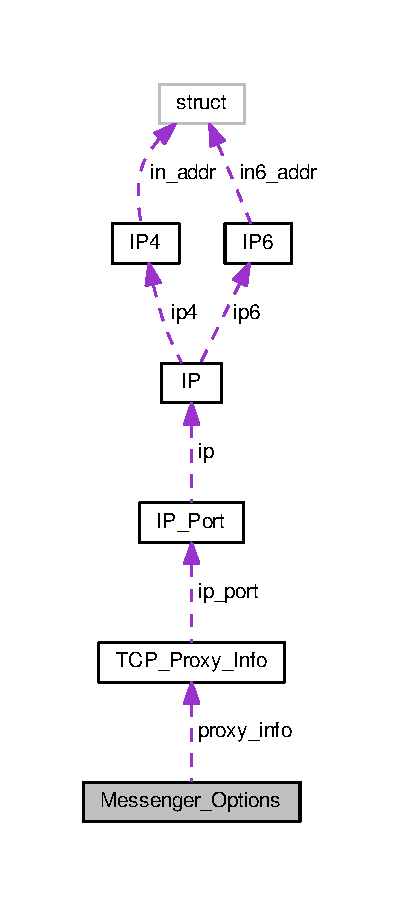
\includegraphics[width=192pt]{struct_messenger___options__coll__graph}
\end{center}
\end{figure}
\subsection*{Data Fields}
\begin{DoxyCompactItemize}
\item 
\hypertarget{struct_messenger___options_abf85a84f394474115b9f45f037ad3378}{uint8\+\_\+t {\bfseries ipv6enabled}}\label{struct_messenger___options_abf85a84f394474115b9f45f037ad3378}

\item 
\hypertarget{struct_messenger___options_a1510f9751065ec1a6d485c4b3072b9d7}{uint8\+\_\+t {\bfseries udp\+\_\+disabled}}\label{struct_messenger___options_a1510f9751065ec1a6d485c4b3072b9d7}

\item 
\hypertarget{struct_messenger___options_aa737023350cf47e63993e3b4dc9a7472}{\hyperlink{struct_t_c_p___proxy___info}{T\+C\+P\+\_\+\+Proxy\+\_\+\+Info} {\bfseries proxy\+\_\+info}}\label{struct_messenger___options_aa737023350cf47e63993e3b4dc9a7472}

\item 
\hypertarget{struct_messenger___options_a6a840950904ae4d13e6726cf5f341fc0}{uint16\+\_\+t {\bfseries port\+\_\+range} \mbox{[}2\mbox{]}}\label{struct_messenger___options_a6a840950904ae4d13e6726cf5f341fc0}

\item 
\hypertarget{struct_messenger___options_a9f404f426cc09060b42b9a61523cc573}{uint16\+\_\+t {\bfseries tcp\+\_\+server\+\_\+port}}\label{struct_messenger___options_a9f404f426cc09060b42b9a61523cc573}

\end{DoxyCompactItemize}


\subsection{Detailed Description}


Definition at line 68 of file Messenger.\+h.



The documentation for this struct was generated from the following file\+:\begin{DoxyCompactItemize}
\item 
toxcore/Messenger.\+h\end{DoxyCompactItemize}

\hypertarget{struct_n_a_t}{\section{N\+A\+T Struct Reference}
\label{struct_n_a_t}\index{N\+A\+T@{N\+A\+T}}
}
\subsection*{Data Fields}
\begin{DoxyCompactItemize}
\item 
\hypertarget{struct_n_a_t_a40495f11f0e91fcea43d57248e202ea3}{uint8\+\_\+t {\bfseries hole\+\_\+punching}}\label{struct_n_a_t_a40495f11f0e91fcea43d57248e202ea3}

\item 
\hypertarget{struct_n_a_t_aeb4b0f7724adb0857b15e0f34e95ecca}{uint32\+\_\+t {\bfseries punching\+\_\+index}}\label{struct_n_a_t_aeb4b0f7724adb0857b15e0f34e95ecca}

\item 
\hypertarget{struct_n_a_t_a852b5b4a6ac0e351887ab6dde3e3fcc5}{uint32\+\_\+t {\bfseries tries}}\label{struct_n_a_t_a852b5b4a6ac0e351887ab6dde3e3fcc5}

\item 
\hypertarget{struct_n_a_t_a1d36817a78a0e261e7ca0982e17aa4ee}{uint32\+\_\+t {\bfseries punching\+\_\+index2}}\label{struct_n_a_t_a1d36817a78a0e261e7ca0982e17aa4ee}

\item 
\hypertarget{struct_n_a_t_ab8cadc230283568e7aeb303691d8e374}{uint64\+\_\+t {\bfseries punching\+\_\+timestamp}}\label{struct_n_a_t_ab8cadc230283568e7aeb303691d8e374}

\item 
\hypertarget{struct_n_a_t_a237df5177fc9db865722933b5b6468ea}{uint64\+\_\+t {\bfseries recv\+N\+A\+Tping\+\_\+timestamp}}\label{struct_n_a_t_a237df5177fc9db865722933b5b6468ea}

\item 
\hypertarget{struct_n_a_t_addd9408d04ff8e05c569651b299f1b1b}{uint64\+\_\+t {\bfseries N\+A\+Tping\+\_\+id}}\label{struct_n_a_t_addd9408d04ff8e05c569651b299f1b1b}

\item 
\hypertarget{struct_n_a_t_a20937663f98914b69bb73f938deed531}{uint64\+\_\+t {\bfseries N\+A\+Tping\+\_\+timestamp}}\label{struct_n_a_t_a20937663f98914b69bb73f938deed531}

\end{DoxyCompactItemize}


\subsection{Detailed Description}


Definition at line 114 of file D\+H\+T.\+h.



The documentation for this struct was generated from the following file\+:\begin{DoxyCompactItemize}
\item 
toxcore/D\+H\+T.\+h\end{DoxyCompactItemize}

\hypertarget{struct_net___crypto}{\section{Net\+\_\+\+Crypto Struct Reference}
\label{struct_net___crypto}\index{Net\+\_\+\+Crypto@{Net\+\_\+\+Crypto}}
}


Collaboration diagram for Net\+\_\+\+Crypto\+:\nopagebreak
\begin{figure}[H]
\begin{center}
\leavevmode
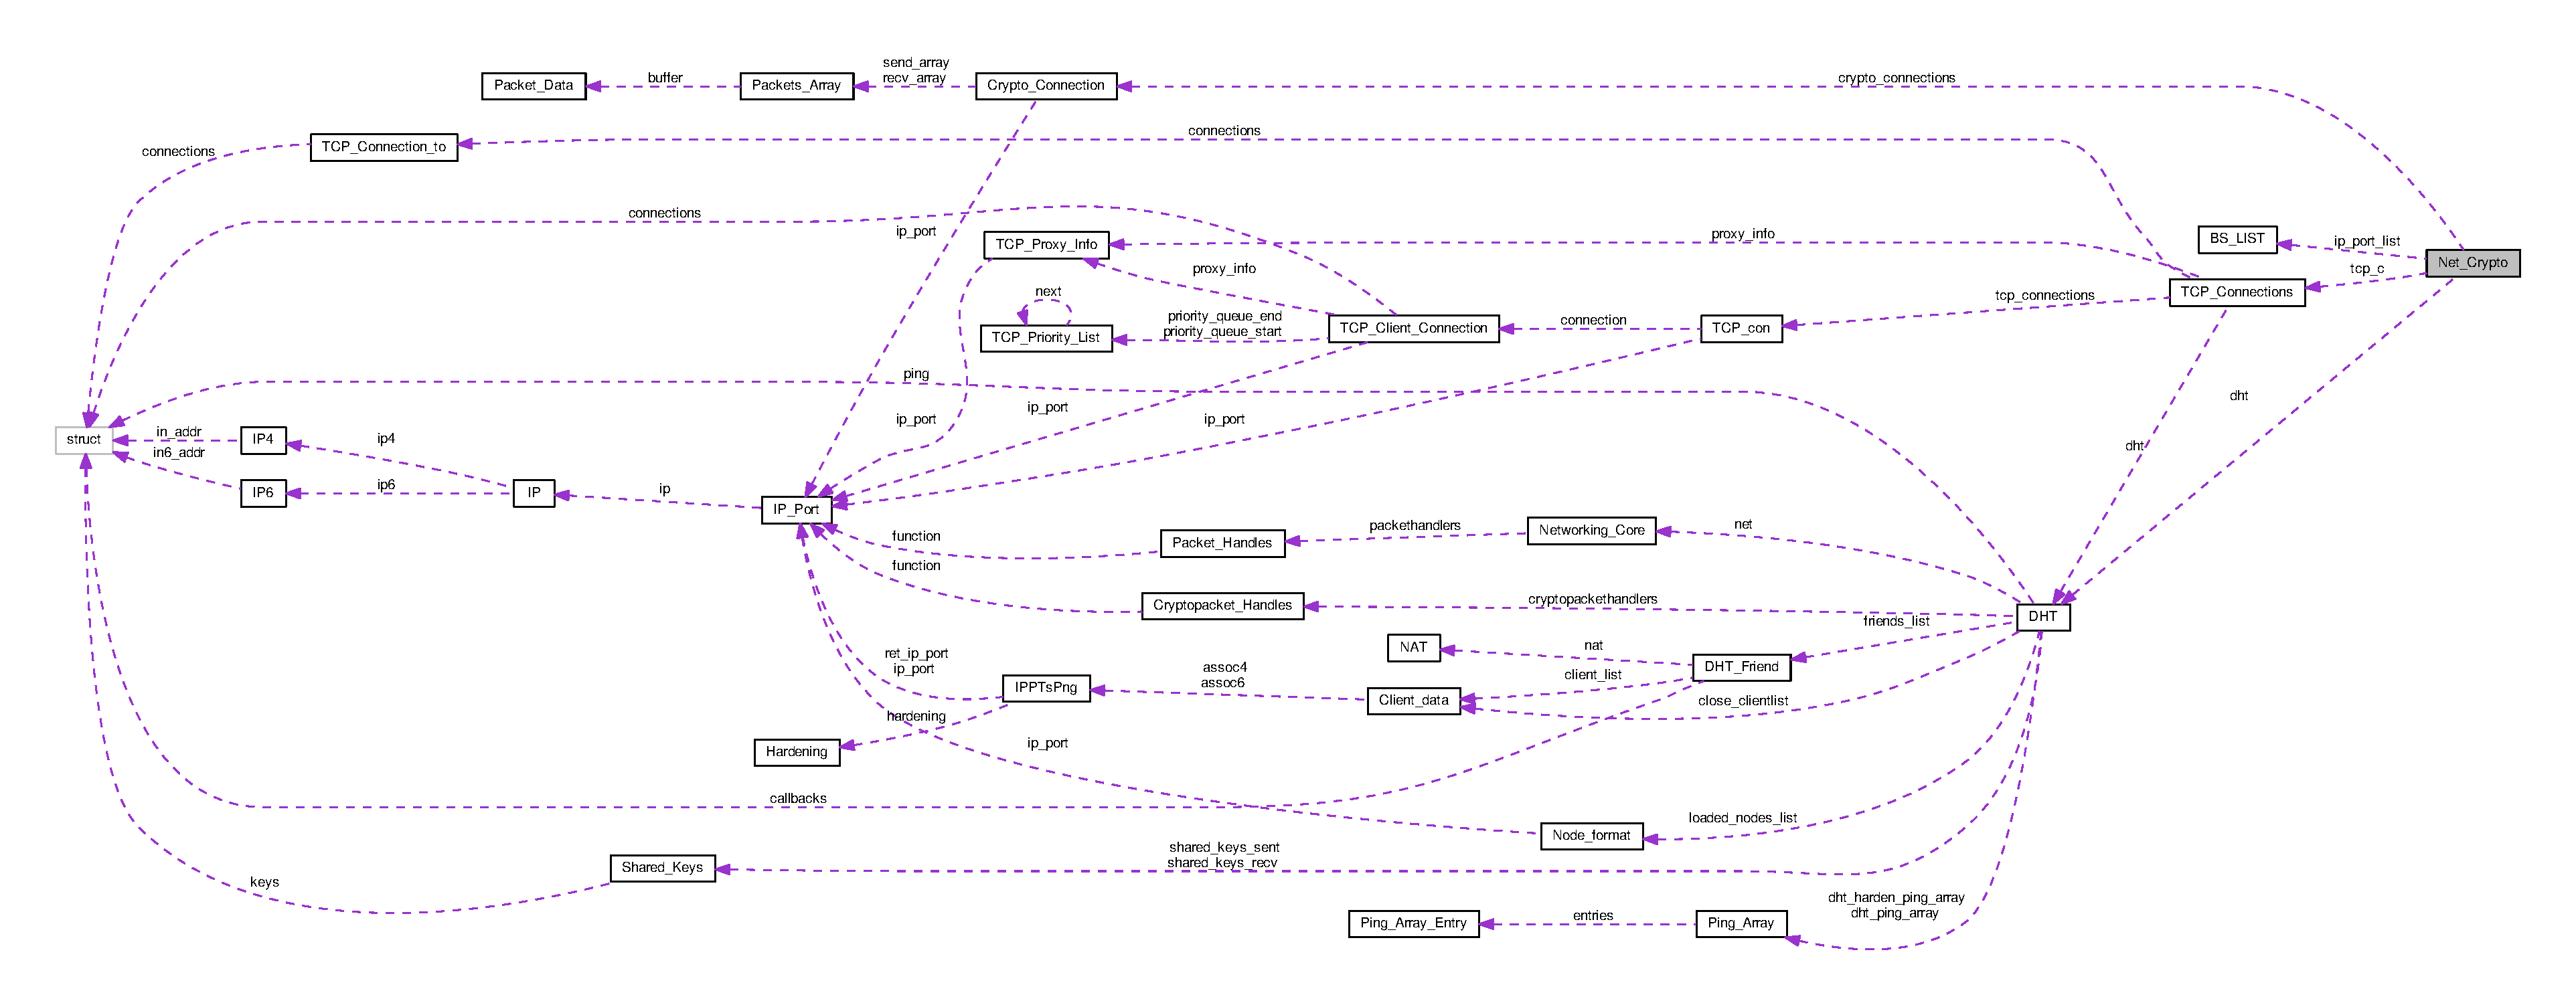
\includegraphics[width=350pt]{struct_net___crypto__coll__graph}
\end{center}
\end{figure}
\subsection*{Data Fields}
\begin{DoxyCompactItemize}
\item 
\hypertarget{struct_net___crypto_a8b3d6ce8745acc52695e252bdb1531b6}{\hyperlink{struct_d_h_t}{D\+H\+T} $\ast$ {\bfseries dht}}\label{struct_net___crypto_a8b3d6ce8745acc52695e252bdb1531b6}

\item 
\hypertarget{struct_net___crypto_a179982a02be89eaf6617ed81bd3c0961}{\hyperlink{struct_t_c_p___connections}{T\+C\+P\+\_\+\+Connections} $\ast$ {\bfseries tcp\+\_\+c}}\label{struct_net___crypto_a179982a02be89eaf6617ed81bd3c0961}

\item 
\hypertarget{struct_net___crypto_a13fdc865b8a114466ba136f5390ec1b2}{\hyperlink{struct_crypto___connection}{Crypto\+\_\+\+Connection} $\ast$ {\bfseries crypto\+\_\+connections}}\label{struct_net___crypto_a13fdc865b8a114466ba136f5390ec1b2}

\item 
\hypertarget{struct_net___crypto_a2e8f7f4dff2f2fc4ac2cc32b0c886974}{pthread\+\_\+mutex\+\_\+t {\bfseries tcp\+\_\+mutex}}\label{struct_net___crypto_a2e8f7f4dff2f2fc4ac2cc32b0c886974}

\item 
\hypertarget{struct_net___crypto_a213135bf3b5b80b1cfe99b27dc42815e}{pthread\+\_\+mutex\+\_\+t {\bfseries connections\+\_\+mutex}}\label{struct_net___crypto_a213135bf3b5b80b1cfe99b27dc42815e}

\item 
\hypertarget{struct_net___crypto_ab5be057850e1cee67902276a69900326}{unsigned int {\bfseries connection\+\_\+use\+\_\+counter}}\label{struct_net___crypto_ab5be057850e1cee67902276a69900326}

\item 
\hypertarget{struct_net___crypto_a9c91c3c65885a2bd39d0f864b9a5ddb9}{uint32\+\_\+t {\bfseries crypto\+\_\+connections\+\_\+length}}\label{struct_net___crypto_a9c91c3c65885a2bd39d0f864b9a5ddb9}

\item 
\hypertarget{struct_net___crypto_ae726df8bdc26380e5a6c3187a00d6881}{uint8\+\_\+t {\bfseries self\+\_\+public\+\_\+key} \mbox{[}crypto\+\_\+box\+\_\+\+P\+U\+B\+L\+I\+C\+K\+E\+Y\+B\+Y\+T\+E\+S\mbox{]}}\label{struct_net___crypto_ae726df8bdc26380e5a6c3187a00d6881}

\item 
\hypertarget{struct_net___crypto_aa05050f86513ff53fe9da81f73c72267}{uint8\+\_\+t {\bfseries self\+\_\+secret\+\_\+key} \mbox{[}crypto\+\_\+box\+\_\+\+S\+E\+C\+R\+E\+T\+K\+E\+Y\+B\+Y\+T\+E\+S\mbox{]}}\label{struct_net___crypto_aa05050f86513ff53fe9da81f73c72267}

\item 
\hypertarget{struct_net___crypto_ab9f2ff47bc0b1e5110202a6e4be86390}{uint8\+\_\+t {\bfseries secret\+\_\+symmetric\+\_\+key} \mbox{[}crypto\+\_\+box\+\_\+\+K\+E\+Y\+B\+Y\+T\+E\+S\mbox{]}}\label{struct_net___crypto_ab9f2ff47bc0b1e5110202a6e4be86390}

\item 
\hypertarget{struct_net___crypto_a4e2c131b4a4b4ccb2acc140c29c628be}{int($\ast$ {\bfseries new\+\_\+connection\+\_\+callback} )(void $\ast$object, \hyperlink{struct_new___connection}{New\+\_\+\+Connection} $\ast$n\+\_\+c)}\label{struct_net___crypto_a4e2c131b4a4b4ccb2acc140c29c628be}

\item 
\hypertarget{struct_net___crypto_af28bac95ede5cab8426b07e02dd1a1b0}{void $\ast$ {\bfseries new\+\_\+connection\+\_\+callback\+\_\+object}}\label{struct_net___crypto_af28bac95ede5cab8426b07e02dd1a1b0}

\item 
\hypertarget{struct_net___crypto_a86823a02e323235811eada4755e3f81e}{uint32\+\_\+t {\bfseries current\+\_\+sleep\+\_\+time}}\label{struct_net___crypto_a86823a02e323235811eada4755e3f81e}

\item 
\hypertarget{struct_net___crypto_ae8cfe94df9c9030bbc525010603450ac}{\hyperlink{struct_b_s___l_i_s_t}{B\+S\+\_\+\+L\+I\+S\+T} {\bfseries ip\+\_\+port\+\_\+list}}\label{struct_net___crypto_ae8cfe94df9c9030bbc525010603450ac}

\end{DoxyCompactItemize}


\subsection{Detailed Description}


Definition at line 177 of file net\+\_\+crypto.\+h.



The documentation for this struct was generated from the following file\+:\begin{DoxyCompactItemize}
\item 
toxcore/net\+\_\+crypto.\+h\end{DoxyCompactItemize}

\hypertarget{struct_networking___core}{\section{Networking\+\_\+\+Core Struct Reference}
\label{struct_networking___core}\index{Networking\+\_\+\+Core@{Networking\+\_\+\+Core}}
}


Collaboration diagram for Networking\+\_\+\+Core\+:
\nopagebreak
\begin{figure}[H]
\begin{center}
\leavevmode
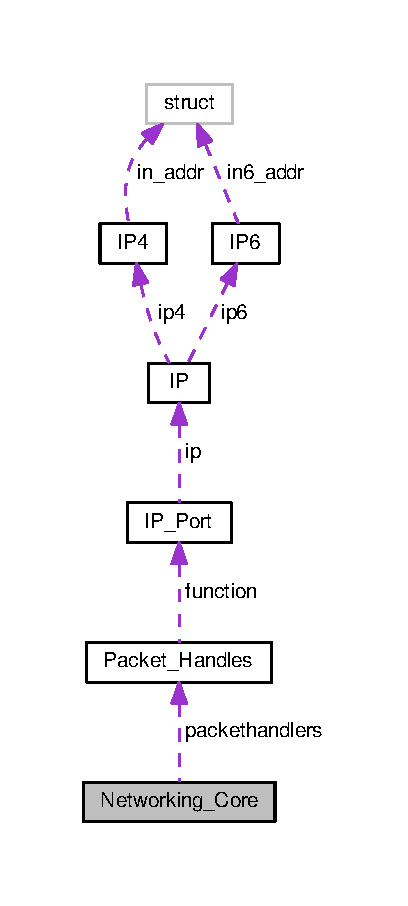
\includegraphics[width=196pt]{struct_networking___core__coll__graph}
\end{center}
\end{figure}
\subsection*{Data Fields}
\begin{DoxyCompactItemize}
\item 
\hypertarget{struct_networking___core_acf65b41b1fc6f52a40016a2329a8ba30}{\hyperlink{struct_packet___handles}{Packet\+\_\+\+Handles} {\bfseries packethandlers} \mbox{[}256\mbox{]}}\label{struct_networking___core_acf65b41b1fc6f52a40016a2329a8ba30}

\item 
\hypertarget{struct_networking___core_a59fa33606a579e9080aced9a5d2659de}{sa\+\_\+family\+\_\+t {\bfseries family}}\label{struct_networking___core_a59fa33606a579e9080aced9a5d2659de}

\item 
\hypertarget{struct_networking___core_a8e0798404bf2cf5dabb84c5ba9a4f236}{uint16\+\_\+t {\bfseries port}}\label{struct_networking___core_a8e0798404bf2cf5dabb84c5ba9a4f236}

\item 
\hypertarget{struct_networking___core_a35b19d84fb632ca8ce5cab237f7089a5}{sock\+\_\+t {\bfseries sock}}\label{struct_networking___core_a35b19d84fb632ca8ce5cab237f7089a5}

\end{DoxyCompactItemize}


\subsection{Detailed Description}


Definition at line 296 of file network.\+h.



The documentation for this struct was generated from the following file\+:\begin{DoxyCompactItemize}
\item 
toxcore/network.\+h\end{DoxyCompactItemize}

\hypertarget{struct_new___connection}{\section{New\+\_\+\+Connection Struct Reference}
\label{struct_new___connection}\index{New\+\_\+\+Connection@{New\+\_\+\+Connection}}
}


Collaboration diagram for New\+\_\+\+Connection\+:
\nopagebreak
\begin{figure}[H]
\begin{center}
\leavevmode
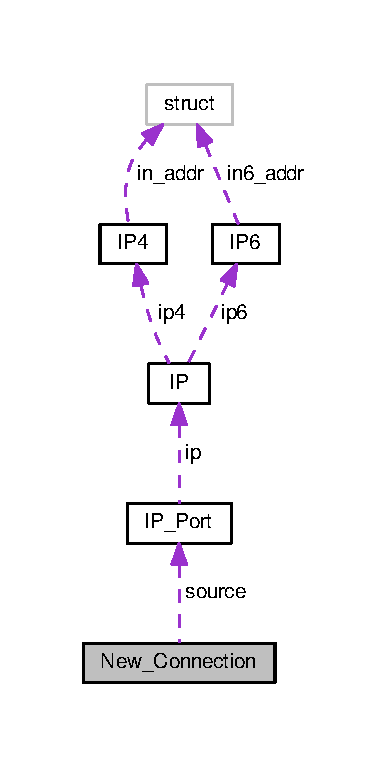
\includegraphics[width=186pt]{struct_new___connection__coll__graph}
\end{center}
\end{figure}
\subsection*{Data Fields}
\begin{DoxyCompactItemize}
\item 
\hypertarget{struct_new___connection_afffde330c649378add9a507c9c151586}{\hyperlink{struct_i_p___port}{I\+P\+\_\+\+Port} {\bfseries source}}\label{struct_new___connection_afffde330c649378add9a507c9c151586}

\item 
\hypertarget{struct_new___connection_aaa806bb1136fb3d4b5d8d8970b596ff7}{uint8\+\_\+t {\bfseries public\+\_\+key} \mbox{[}crypto\+\_\+box\+\_\+\+P\+U\+B\+L\+I\+C\+K\+E\+Y\+B\+Y\+T\+E\+S\mbox{]}}\label{struct_new___connection_aaa806bb1136fb3d4b5d8d8970b596ff7}

\item 
\hypertarget{struct_new___connection_ab2ecaa07625ad0ed5e07d3a1f0dcc939}{uint8\+\_\+t {\bfseries dht\+\_\+public\+\_\+key} \mbox{[}crypto\+\_\+box\+\_\+\+P\+U\+B\+L\+I\+C\+K\+E\+Y\+B\+Y\+T\+E\+S\mbox{]}}\label{struct_new___connection_ab2ecaa07625ad0ed5e07d3a1f0dcc939}

\item 
\hypertarget{struct_new___connection_aae0467706f97aa3ef23e5dc9c3c199d7}{uint8\+\_\+t {\bfseries recv\+\_\+nonce} \mbox{[}crypto\+\_\+box\+\_\+\+N\+O\+N\+C\+E\+B\+Y\+T\+E\+S\mbox{]}}\label{struct_new___connection_aae0467706f97aa3ef23e5dc9c3c199d7}

\item 
\hypertarget{struct_new___connection_ac040d4ba2a22ee327952009e7396bb2f}{uint8\+\_\+t {\bfseries peersessionpublic\+\_\+key} \mbox{[}crypto\+\_\+box\+\_\+\+P\+U\+B\+L\+I\+C\+K\+E\+Y\+B\+Y\+T\+E\+S\mbox{]}}\label{struct_new___connection_ac040d4ba2a22ee327952009e7396bb2f}

\item 
\hypertarget{struct_new___connection_a78fb2cbe7af4d12847f2f044c35e7823}{uint8\+\_\+t $\ast$ {\bfseries cookie}}\label{struct_new___connection_a78fb2cbe7af4d12847f2f044c35e7823}

\item 
\hypertarget{struct_new___connection_a801672aeddedd60f76a667a2275a95ce}{uint8\+\_\+t {\bfseries cookie\+\_\+length}}\label{struct_new___connection_a801672aeddedd60f76a667a2275a95ce}

\end{DoxyCompactItemize}


\subsection{Detailed Description}


Definition at line 167 of file net\+\_\+crypto.\+h.



The documentation for this struct was generated from the following file\+:\begin{DoxyCompactItemize}
\item 
toxcore/net\+\_\+crypto.\+h\end{DoxyCompactItemize}

\hypertarget{struct_node__format}{\section{Node\+\_\+format Struct Reference}
\label{struct_node__format}\index{Node\+\_\+format@{Node\+\_\+format}}
}


{\ttfamily \#include $<$D\+H\+T.\+h$>$}



Collaboration diagram for Node\+\_\+format\+:
\nopagebreak
\begin{figure}[H]
\begin{center}
\leavevmode
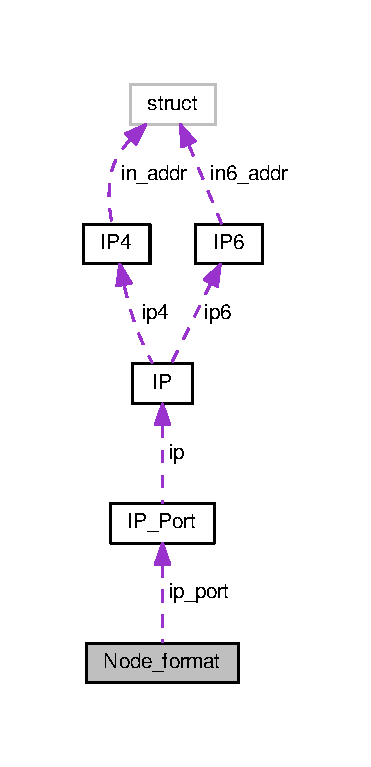
\includegraphics[width=178pt]{d0/df8/struct_node__format__coll__graph}
\end{center}
\end{figure}
\subsection*{Data Fields}
\begin{DoxyCompactItemize}
\item 
uint8\+\_\+t \hyperlink{struct_node__format_aaa806bb1136fb3d4b5d8d8970b596ff7}{public\+\_\+key} \mbox{[}crypto\+\_\+box\+\_\+\+P\+U\+B\+L\+I\+C\+K\+E\+Y\+B\+Y\+T\+E\+S\mbox{]}
\item 
\hyperlink{struct_i_p___port}{I\+P\+\_\+\+Port} \hyperlink{struct_node__format_a86e2a5a56c0dd22df6e8b8a10e40f9e4}{ip\+\_\+port}
\end{DoxyCompactItemize}


\subsection{Detailed Description}


Definition at line 147 of file D\+H\+T.\+h.



\subsection{Field Documentation}
\hypertarget{struct_node__format_a86e2a5a56c0dd22df6e8b8a10e40f9e4}{\index{Node\+\_\+format@{Node\+\_\+format}!ip\+\_\+port@{ip\+\_\+port}}
\index{ip\+\_\+port@{ip\+\_\+port}!Node\+\_\+format@{Node\+\_\+format}}
\subsubsection[{ip\+\_\+port}]{\setlength{\rightskip}{0pt plus 5cm}{\bf I\+P\+\_\+\+Port} ip\+\_\+port}}\label{struct_node__format_a86e2a5a56c0dd22df6e8b8a10e40f9e4}


Definition at line 149 of file D\+H\+T.\+h.



Referenced by add\+\_\+to\+\_\+ping(), closelist\+\_\+nodes(), connect\+\_\+to\+\_\+saved\+\_\+tcp\+\_\+relays(), create\+\_\+onion\+\_\+path(), D\+H\+T\+\_\+connect\+\_\+after\+\_\+load(), D\+H\+T\+\_\+save(), do\+\_\+friend(), do\+\_\+hardening(), do\+\_\+messenger(), do\+\_\+to\+\_\+ping(), friend\+\_\+add\+\_\+tcp\+\_\+relay(), get\+\_\+close\+\_\+nodes(), get\+\_\+close\+\_\+nodes\+\_\+inner(), getnodes(), handle\+\_\+dhtpk\+\_\+announce(), handle\+\_\+hardening(), handle\+\_\+sendnodes\+\_\+ipv6(), is\+\_\+path\+\_\+used(), messenger\+\_\+load\+\_\+state\+\_\+callback(), onion\+\_\+add\+\_\+bs\+\_\+path\+\_\+node(), onion\+\_\+add\+\_\+path\+\_\+node(), onion\+\_\+path\+\_\+to\+\_\+nodes(), random\+\_\+nodes\+\_\+path\+\_\+onion(), send\+\_\+announce\+\_\+request(), send\+\_\+hardening\+\_\+getnode\+\_\+res(), send\+\_\+hardening\+\_\+req(), sent\+\_\+getnode\+\_\+to\+\_\+node(), S\+T\+A\+R\+T\+\_\+\+T\+E\+S\+T(), tcp\+\_\+copy\+\_\+connected\+\_\+relays(), and unpack\+\_\+nodes().

\hypertarget{struct_node__format_aaa806bb1136fb3d4b5d8d8970b596ff7}{\index{Node\+\_\+format@{Node\+\_\+format}!public\+\_\+key@{public\+\_\+key}}
\index{public\+\_\+key@{public\+\_\+key}!Node\+\_\+format@{Node\+\_\+format}}
\subsubsection[{public\+\_\+key}]{\setlength{\rightskip}{0pt plus 5cm}uint8\+\_\+t public\+\_\+key\mbox{[}crypto\+\_\+box\+\_\+\+P\+U\+B\+L\+I\+C\+K\+E\+Y\+B\+Y\+T\+E\+S\mbox{]}}}\label{struct_node__format_aaa806bb1136fb3d4b5d8d8970b596ff7}


Definition at line 148 of file D\+H\+T.\+h.



Referenced by add\+\_\+to\+\_\+ping(), connect\+\_\+to\+\_\+saved\+\_\+tcp\+\_\+relays(), create\+\_\+onion\+\_\+path(), D\+H\+T\+\_\+connect\+\_\+after\+\_\+load(), do\+\_\+friend(), do\+\_\+hardening(), do\+\_\+messenger(), do\+\_\+to\+\_\+ping(), friend\+\_\+add\+\_\+tcp\+\_\+relay(), getnodes(), handle\+\_\+dhtpk\+\_\+announce(), handle\+\_\+hardening(), handle\+\_\+sendnodes\+\_\+ipv6(), messenger\+\_\+load\+\_\+state\+\_\+callback(), onion\+\_\+add\+\_\+bs\+\_\+path\+\_\+node(), onion\+\_\+add\+\_\+path\+\_\+node(), send\+\_\+announce\+\_\+request(), send\+\_\+hardening\+\_\+getnode\+\_\+res(), send\+\_\+hardening\+\_\+req(), sent\+\_\+getnode\+\_\+to\+\_\+node(), and S\+T\+A\+R\+T\+\_\+\+T\+E\+S\+T().



The documentation for this struct was generated from the following file\+:\begin{DoxyCompactItemize}
\item 
toxcore/\hyperlink{_d_h_t_8h}{D\+H\+T.\+h}\end{DoxyCompactItemize}

\hypertarget{struct_onion}{\section{Onion Struct Reference}
\label{struct_onion}\index{Onion@{Onion}}
}


Collaboration diagram for Onion\+:
\nopagebreak
\begin{figure}[H]
\begin{center}
\leavevmode
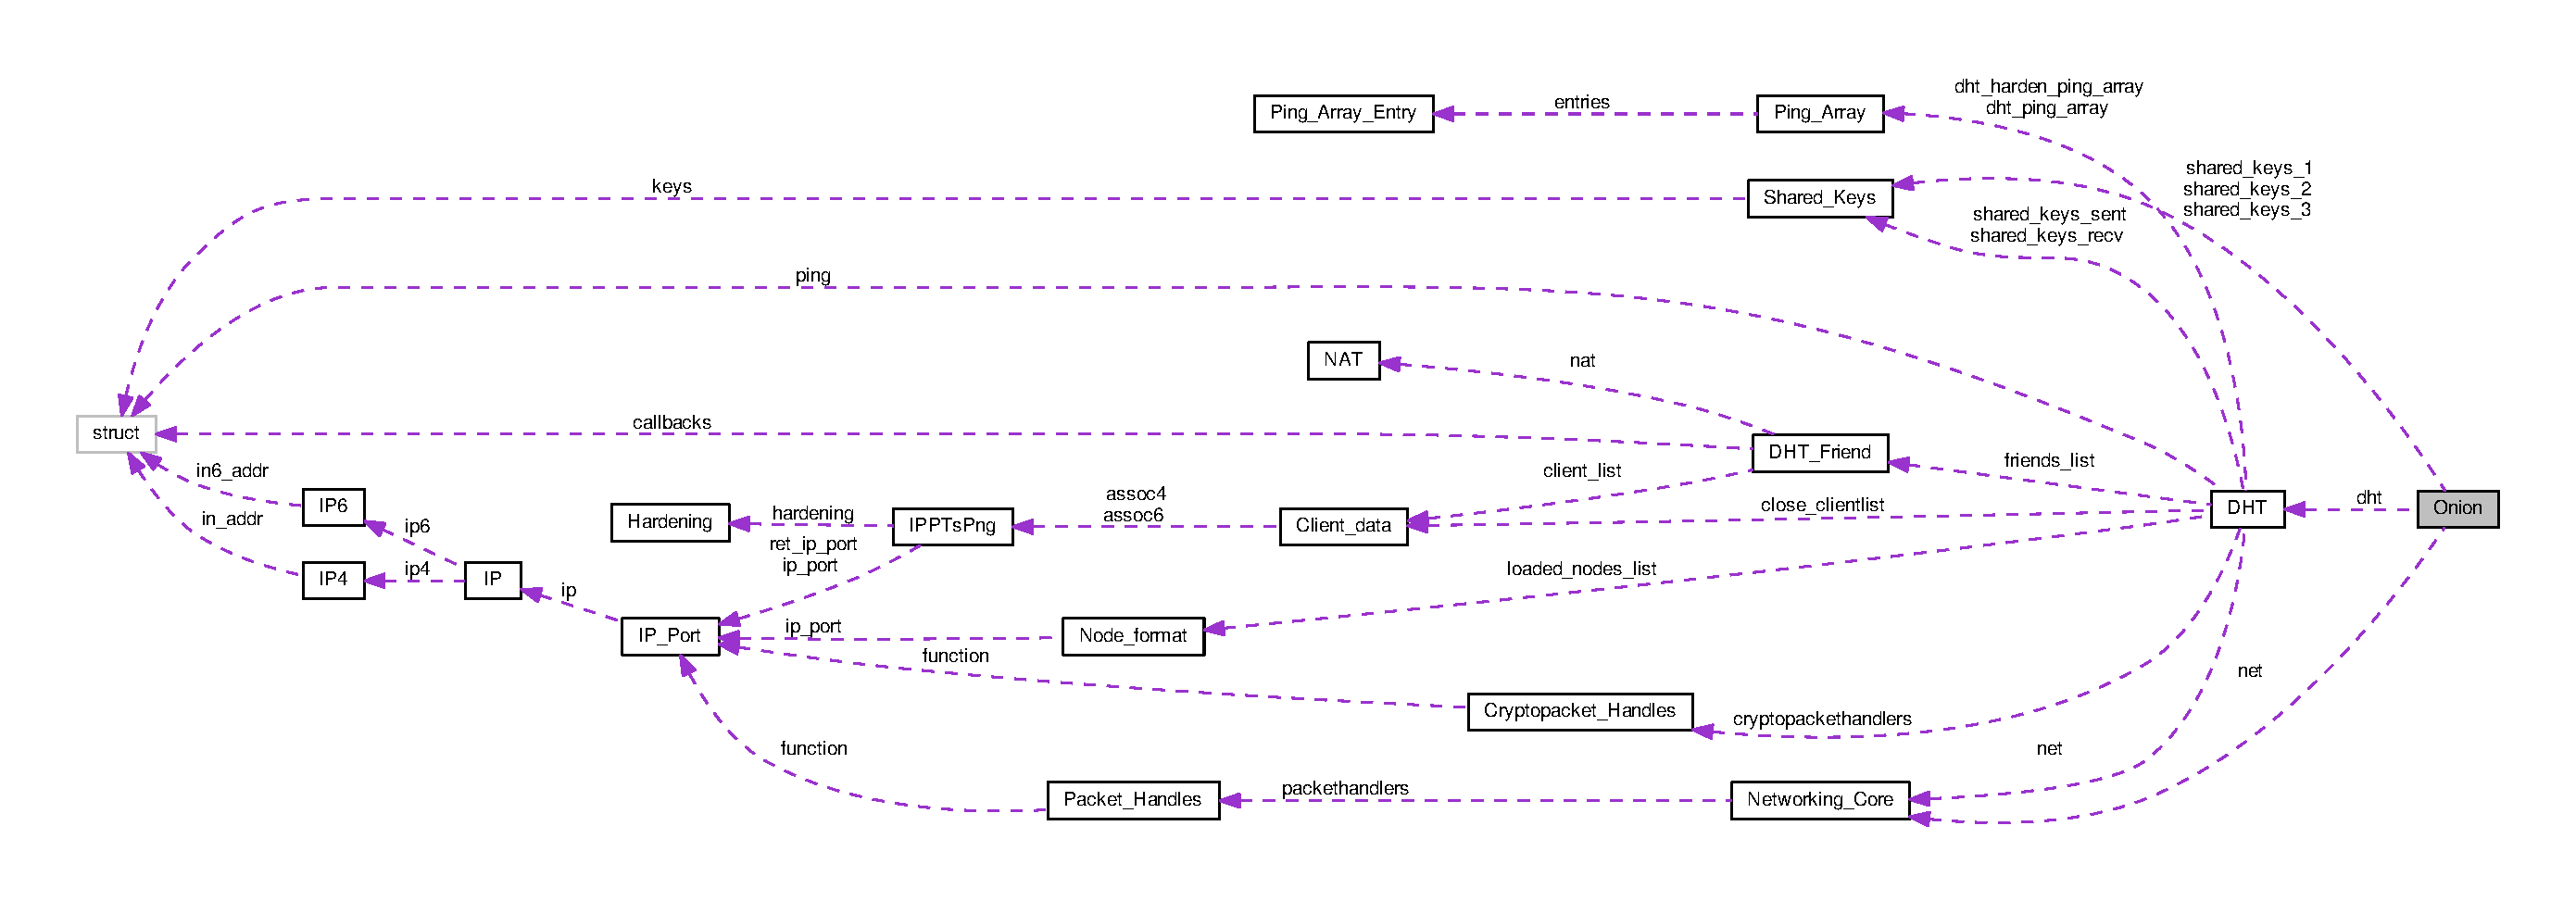
\includegraphics[width=350pt]{struct_onion__coll__graph}
\end{center}
\end{figure}
\subsection*{Data Fields}
\begin{DoxyCompactItemize}
\item 
\hypertarget{struct_onion_a8b3d6ce8745acc52695e252bdb1531b6}{\hyperlink{struct_d_h_t}{D\+H\+T} $\ast$ {\bfseries dht}}\label{struct_onion_a8b3d6ce8745acc52695e252bdb1531b6}

\item 
\hypertarget{struct_onion_aa14ea2f67950f57fe4235d7375a2216c}{\hyperlink{struct_networking___core}{Networking\+\_\+\+Core} $\ast$ {\bfseries net}}\label{struct_onion_aa14ea2f67950f57fe4235d7375a2216c}

\item 
\hypertarget{struct_onion_ab9f2ff47bc0b1e5110202a6e4be86390}{uint8\+\_\+t {\bfseries secret\+\_\+symmetric\+\_\+key} \mbox{[}crypto\+\_\+box\+\_\+\+K\+E\+Y\+B\+Y\+T\+E\+S\mbox{]}}\label{struct_onion_ab9f2ff47bc0b1e5110202a6e4be86390}

\item 
\hypertarget{struct_onion_a465bef81f6478756e5443025b1f2ddfa}{uint64\+\_\+t {\bfseries timestamp}}\label{struct_onion_a465bef81f6478756e5443025b1f2ddfa}

\item 
\hypertarget{struct_onion_a7dc1514173e0fd82d265ebc3a43090ea}{\hyperlink{struct_shared___keys}{Shared\+\_\+\+Keys} {\bfseries shared\+\_\+keys\+\_\+1}}\label{struct_onion_a7dc1514173e0fd82d265ebc3a43090ea}

\item 
\hypertarget{struct_onion_a01ec0631137b85dd55bf0cbb3492e8f5}{\hyperlink{struct_shared___keys}{Shared\+\_\+\+Keys} {\bfseries shared\+\_\+keys\+\_\+2}}\label{struct_onion_a01ec0631137b85dd55bf0cbb3492e8f5}

\item 
\hypertarget{struct_onion_a2c2de8d3552fa4223cbf58557704b977}{\hyperlink{struct_shared___keys}{Shared\+\_\+\+Keys} {\bfseries shared\+\_\+keys\+\_\+3}}\label{struct_onion_a2c2de8d3552fa4223cbf58557704b977}

\item 
\hypertarget{struct_onion_a980753d0df6688333680e95f637eb7a7}{int($\ast$ {\bfseries recv\+\_\+1\+\_\+function} )(void $\ast$, \hyperlink{struct_i_p___port}{I\+P\+\_\+\+Port}, const uint8\+\_\+t $\ast$, uint16\+\_\+t)}\label{struct_onion_a980753d0df6688333680e95f637eb7a7}

\item 
\hypertarget{struct_onion_aa30dff385b8f119ddb95900b2a250a08}{void $\ast$ {\bfseries callback\+\_\+object}}\label{struct_onion_aa30dff385b8f119ddb95900b2a250a08}

\end{DoxyCompactItemize}


\subsection{Detailed Description}


Definition at line 28 of file onion.\+h.



The documentation for this struct was generated from the following file\+:\begin{DoxyCompactItemize}
\item 
toxcore/onion.\+h\end{DoxyCompactItemize}

\hypertarget{struct_onion___announce}{\section{Onion\+\_\+\+Announce Struct Reference}
\label{struct_onion___announce}\index{Onion\+\_\+\+Announce@{Onion\+\_\+\+Announce}}
}


Collaboration diagram for Onion\+\_\+\+Announce\+:\nopagebreak
\begin{figure}[H]
\begin{center}
\leavevmode
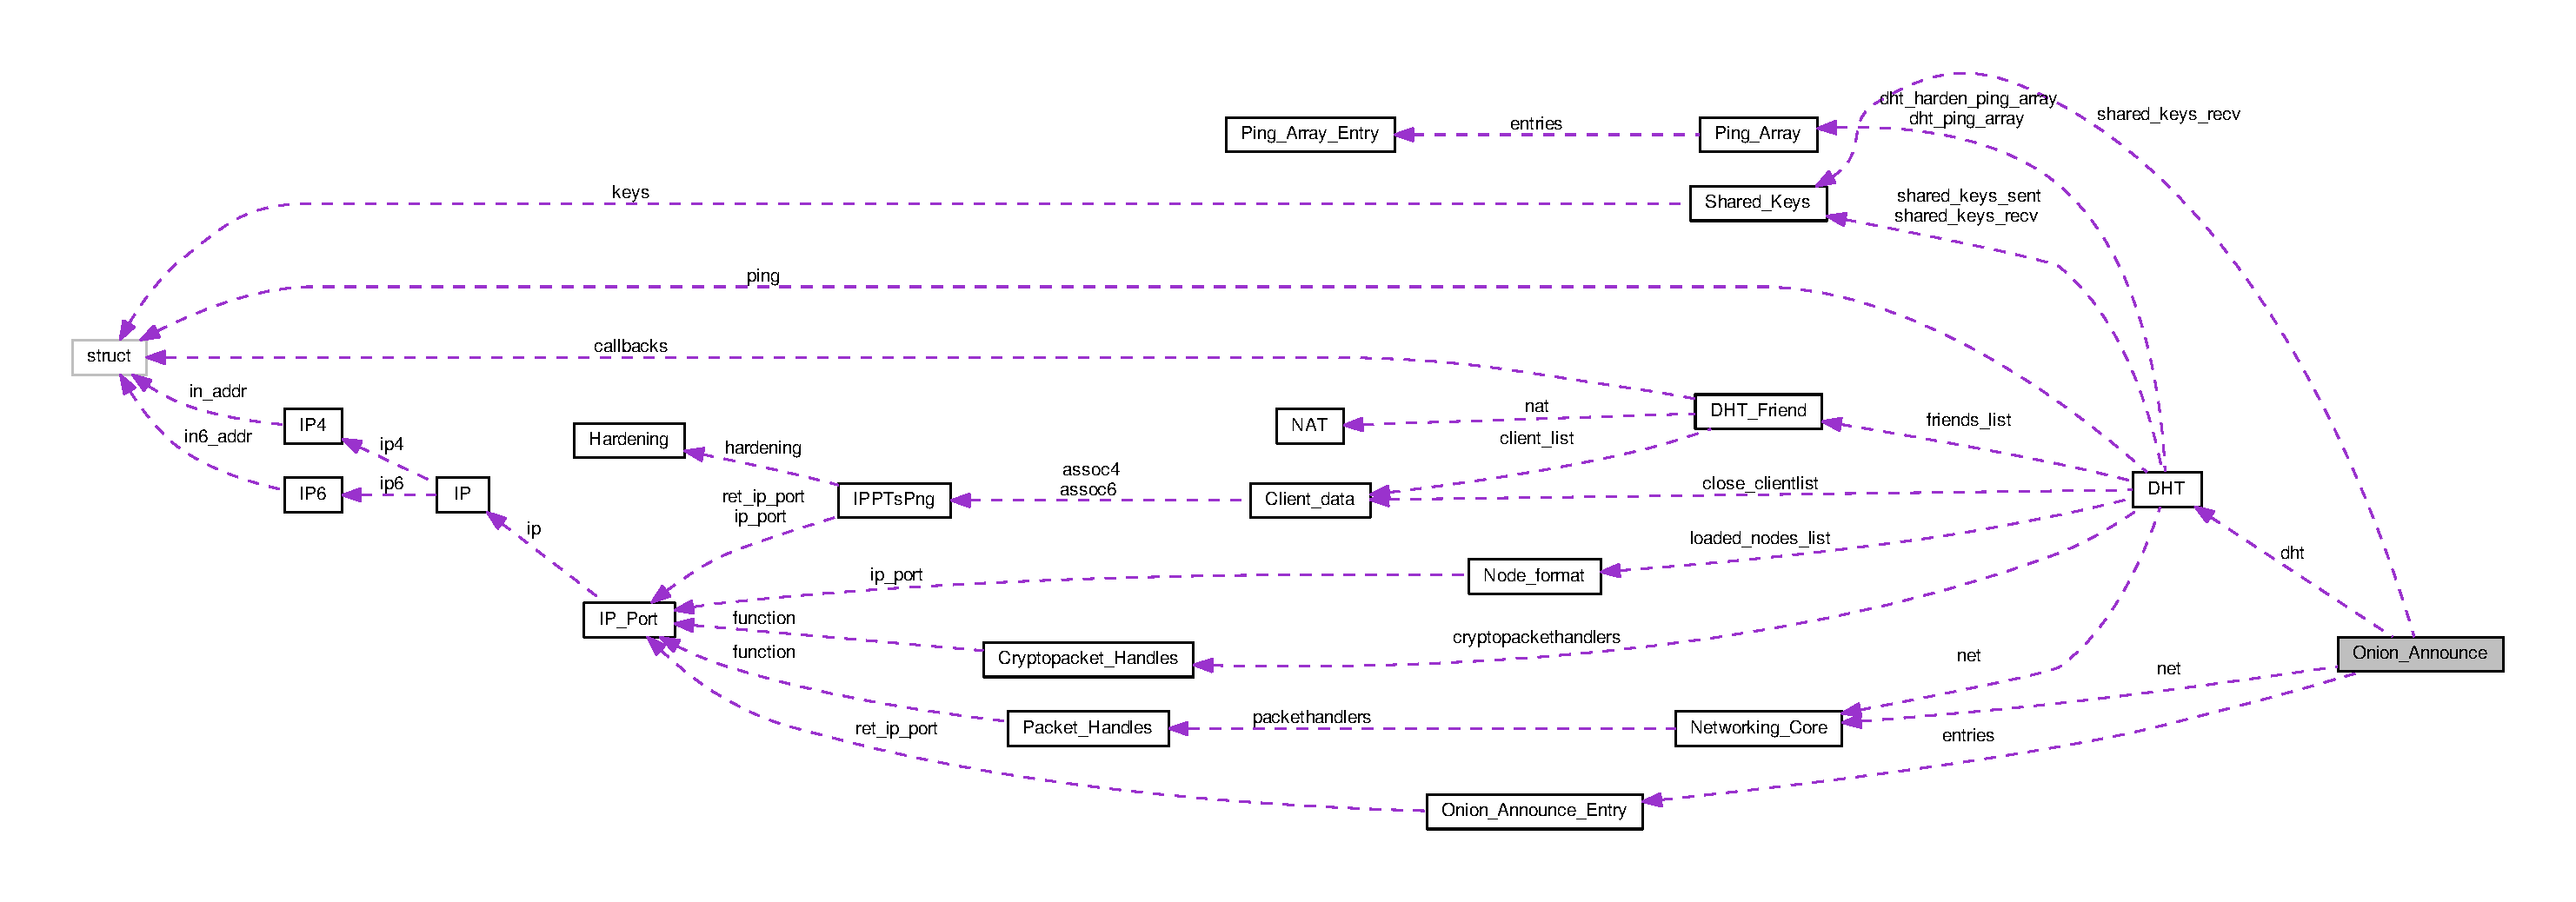
\includegraphics[width=350pt]{struct_onion___announce__coll__graph}
\end{center}
\end{figure}
\subsection*{Data Fields}
\begin{DoxyCompactItemize}
\item 
\hypertarget{struct_onion___announce_a8b3d6ce8745acc52695e252bdb1531b6}{\hyperlink{struct_d_h_t}{D\+H\+T} $\ast$ {\bfseries dht}}\label{struct_onion___announce_a8b3d6ce8745acc52695e252bdb1531b6}

\item 
\hypertarget{struct_onion___announce_aa14ea2f67950f57fe4235d7375a2216c}{\hyperlink{struct_networking___core}{Networking\+\_\+\+Core} $\ast$ {\bfseries net}}\label{struct_onion___announce_aa14ea2f67950f57fe4235d7375a2216c}

\item 
\hypertarget{struct_onion___announce_a2de468d0c9db89713f12f2e7bd984023}{\hyperlink{struct_onion___announce___entry}{Onion\+\_\+\+Announce\+\_\+\+Entry} {\bfseries entries} \mbox{[}O\+N\+I\+O\+N\+\_\+\+A\+N\+N\+O\+U\+N\+C\+E\+\_\+\+M\+A\+X\+\_\+\+E\+N\+T\+R\+I\+E\+S\mbox{]}}\label{struct_onion___announce_a2de468d0c9db89713f12f2e7bd984023}

\item 
\hypertarget{struct_onion___announce_ad4bfea97df71f88d6de4cbf53f301928}{uint8\+\_\+t {\bfseries secret\+\_\+bytes} \mbox{[}crypto\+\_\+box\+\_\+\+K\+E\+Y\+B\+Y\+T\+E\+S\mbox{]}}\label{struct_onion___announce_ad4bfea97df71f88d6de4cbf53f301928}

\item 
\hypertarget{struct_onion___announce_a4c647e235c4b9d2d6d68d760c7cb1b30}{\hyperlink{struct_shared___keys}{Shared\+\_\+\+Keys} {\bfseries shared\+\_\+keys\+\_\+recv}}\label{struct_onion___announce_a4c647e235c4b9d2d6d68d760c7cb1b30}

\end{DoxyCompactItemize}


\subsection{Detailed Description}


Definition at line 56 of file onion\+\_\+announce.\+h.



The documentation for this struct was generated from the following file\+:\begin{DoxyCompactItemize}
\item 
toxcore/onion\+\_\+announce.\+h\end{DoxyCompactItemize}

\hypertarget{struct_onion___announce___entry}{\section{Onion\+\_\+\+Announce\+\_\+\+Entry Struct Reference}
\label{struct_onion___announce___entry}\index{Onion\+\_\+\+Announce\+\_\+\+Entry@{Onion\+\_\+\+Announce\+\_\+\+Entry}}
}


Collaboration diagram for Onion\+\_\+\+Announce\+\_\+\+Entry\+:\nopagebreak
\begin{figure}[H]
\begin{center}
\leavevmode
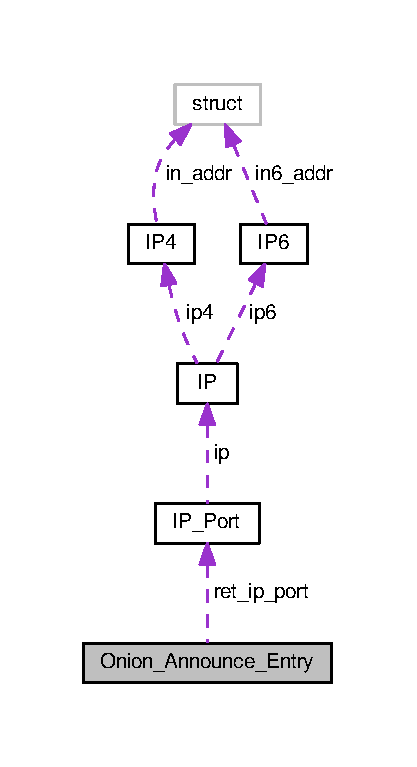
\includegraphics[width=200pt]{struct_onion___announce___entry__coll__graph}
\end{center}
\end{figure}
\subsection*{Data Fields}
\begin{DoxyCompactItemize}
\item 
\hypertarget{struct_onion___announce___entry_aaa806bb1136fb3d4b5d8d8970b596ff7}{uint8\+\_\+t {\bfseries public\+\_\+key} \mbox{[}crypto\+\_\+box\+\_\+\+P\+U\+B\+L\+I\+C\+K\+E\+Y\+B\+Y\+T\+E\+S\mbox{]}}\label{struct_onion___announce___entry_aaa806bb1136fb3d4b5d8d8970b596ff7}

\item 
\hypertarget{struct_onion___announce___entry_a28f2dcc657352ee4855d05ed42e4a4af}{\hyperlink{struct_i_p___port}{I\+P\+\_\+\+Port} {\bfseries ret\+\_\+ip\+\_\+port}}\label{struct_onion___announce___entry_a28f2dcc657352ee4855d05ed42e4a4af}

\item 
\hypertarget{struct_onion___announce___entry_a860a2c4025701999e0d03f73b1863cdd}{uint8\+\_\+t {\bfseries ret} \mbox{[}O\+N\+I\+O\+N\+\_\+\+R\+E\+T\+U\+R\+N\+\_\+3\mbox{]}}\label{struct_onion___announce___entry_a860a2c4025701999e0d03f73b1863cdd}

\item 
\hypertarget{struct_onion___announce___entry_add8f6d39a7818b6d3ff0fca42a0aadf4}{uint8\+\_\+t {\bfseries data\+\_\+public\+\_\+key} \mbox{[}crypto\+\_\+box\+\_\+\+P\+U\+B\+L\+I\+C\+K\+E\+Y\+B\+Y\+T\+E\+S\mbox{]}}\label{struct_onion___announce___entry_add8f6d39a7818b6d3ff0fca42a0aadf4}

\item 
\hypertarget{struct_onion___announce___entry_a5d34a8f2dfe25421b2b473a5fd37b0ed}{uint64\+\_\+t {\bfseries time}}\label{struct_onion___announce___entry_a5d34a8f2dfe25421b2b473a5fd37b0ed}

\end{DoxyCompactItemize}


\subsection{Detailed Description}


Definition at line 48 of file onion\+\_\+announce.\+h.



The documentation for this struct was generated from the following file\+:\begin{DoxyCompactItemize}
\item 
toxcore/onion\+\_\+announce.\+h\end{DoxyCompactItemize}

\hypertarget{struct_onion___client}{\section{Onion\+\_\+\+Client Struct Reference}
\label{struct_onion___client}\index{Onion\+\_\+\+Client@{Onion\+\_\+\+Client}}
}


Collaboration diagram for Onion\+\_\+\+Client\+:\nopagebreak
\begin{figure}[H]
\begin{center}
\leavevmode
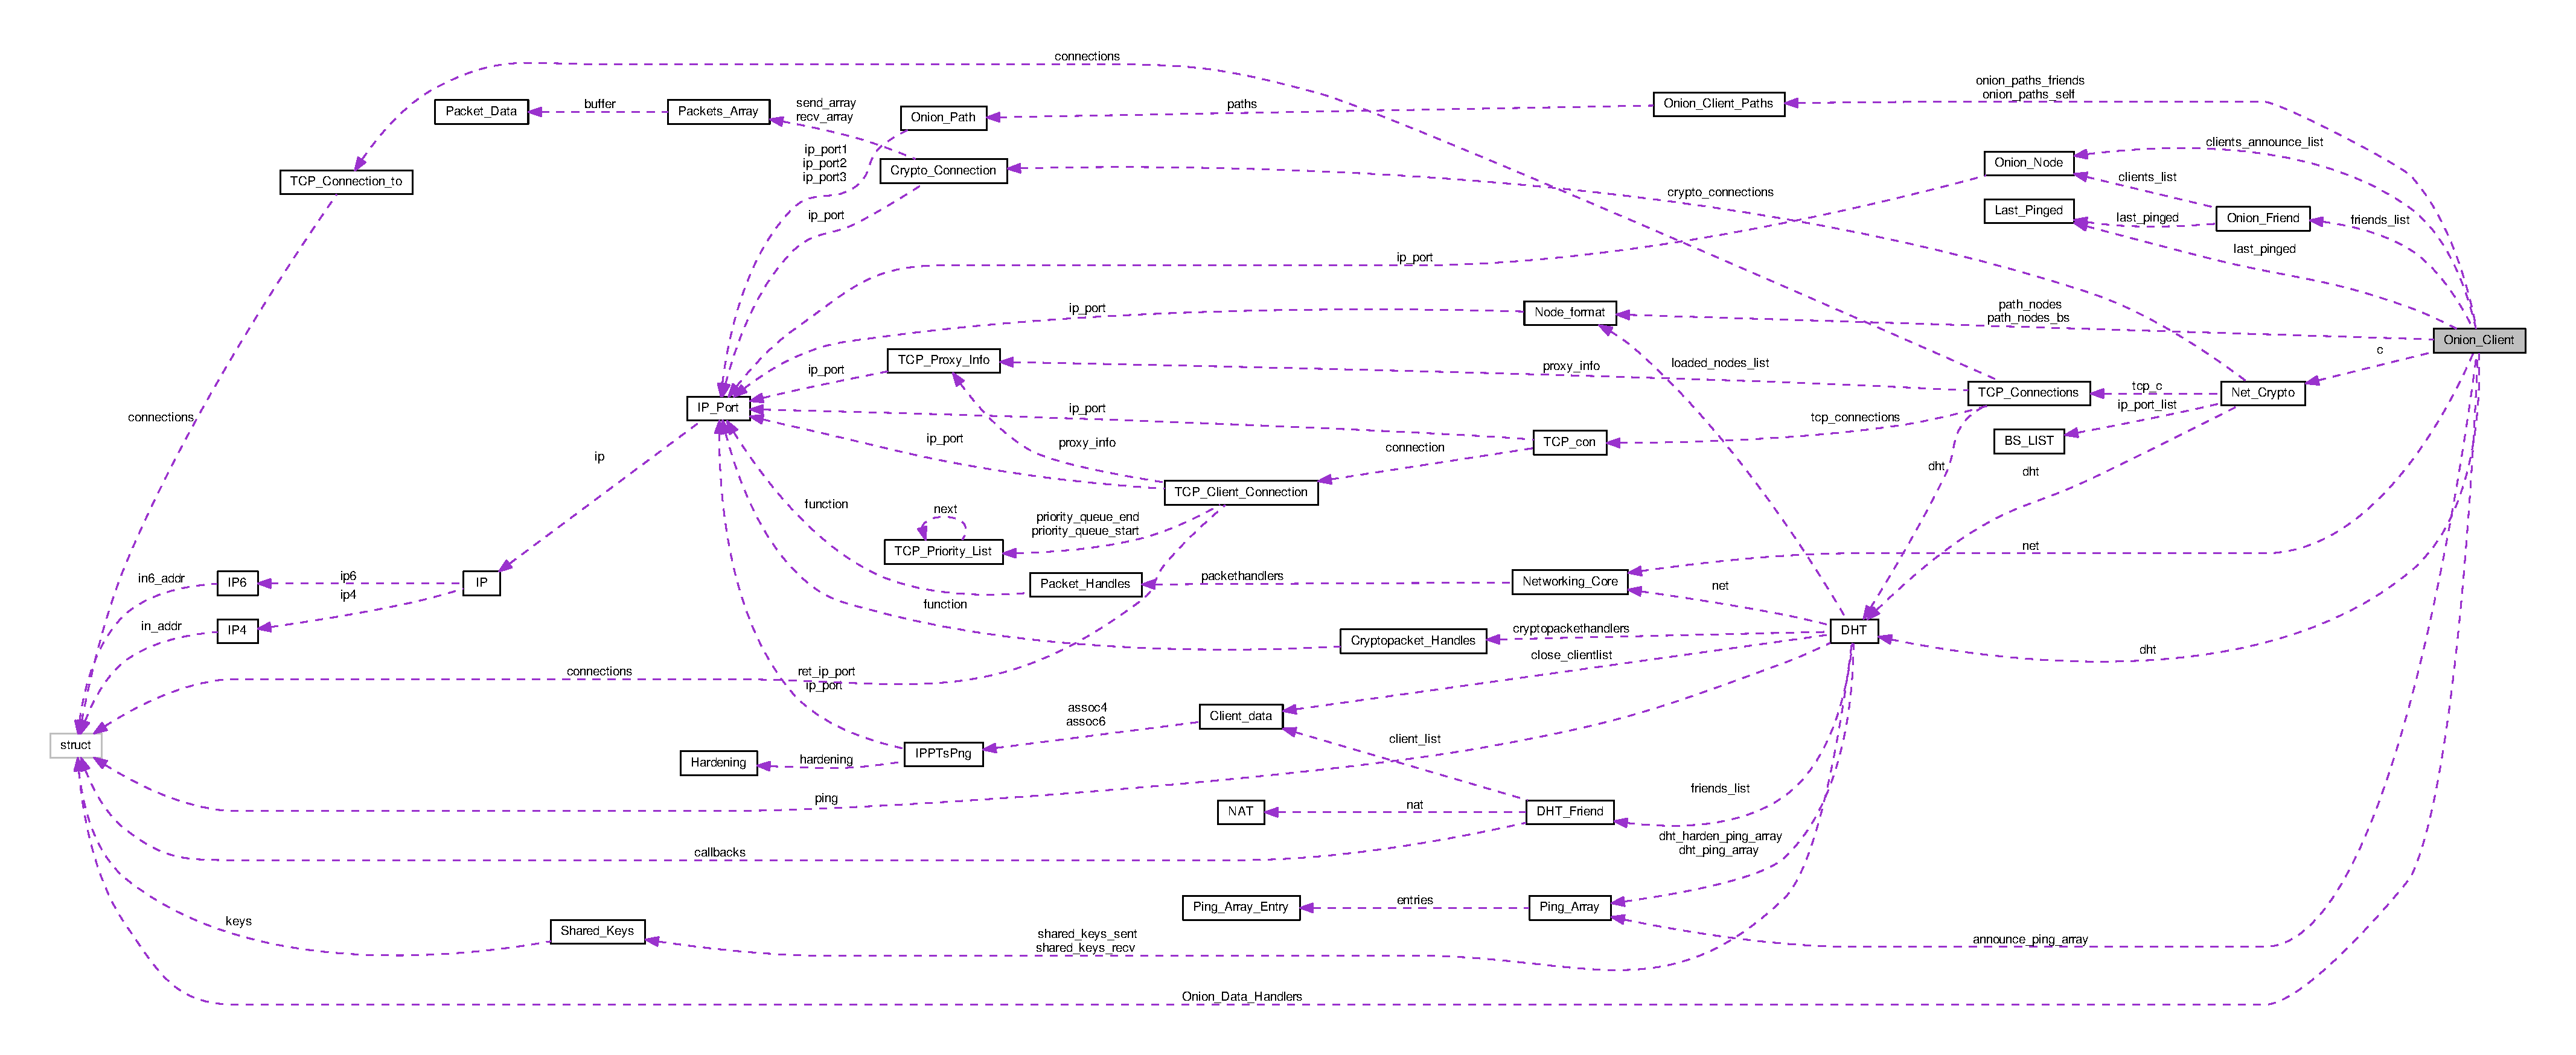
\includegraphics[width=350pt]{struct_onion___client__coll__graph}
\end{center}
\end{figure}
\subsection*{Data Fields}
\begin{DoxyCompactItemize}
\item 
\hypertarget{struct_onion___client_a8b3d6ce8745acc52695e252bdb1531b6}{\hyperlink{struct_d_h_t}{D\+H\+T} $\ast$ {\bfseries dht}}\label{struct_onion___client_a8b3d6ce8745acc52695e252bdb1531b6}

\item 
\hypertarget{struct_onion___client_a0f5b9349eb586149cef9017eed2abdfe}{\hyperlink{struct_net___crypto}{Net\+\_\+\+Crypto} $\ast$ {\bfseries c}}\label{struct_onion___client_a0f5b9349eb586149cef9017eed2abdfe}

\item 
\hypertarget{struct_onion___client_aa14ea2f67950f57fe4235d7375a2216c}{\hyperlink{struct_networking___core}{Networking\+\_\+\+Core} $\ast$ {\bfseries net}}\label{struct_onion___client_aa14ea2f67950f57fe4235d7375a2216c}

\item 
\hypertarget{struct_onion___client_ad2d8940ddd914d8b046938ef4f9d313d}{\hyperlink{struct_onion___friend}{Onion\+\_\+\+Friend} $\ast$ {\bfseries friends\+\_\+list}}\label{struct_onion___client_ad2d8940ddd914d8b046938ef4f9d313d}

\item 
\hypertarget{struct_onion___client_a8ee1f2d7e543bce350c591a8eaac0cf8}{uint16\+\_\+t {\bfseries num\+\_\+friends}}\label{struct_onion___client_a8ee1f2d7e543bce350c591a8eaac0cf8}

\item 
\hypertarget{struct_onion___client_a21a83b6615ce3ab53739031a355aeabd}{\hyperlink{struct_onion___node}{Onion\+\_\+\+Node} {\bfseries clients\+\_\+announce\+\_\+list} \mbox{[}M\+A\+X\+\_\+\+O\+N\+I\+O\+N\+\_\+\+C\+L\+I\+E\+N\+T\+S\mbox{]}}\label{struct_onion___client_a21a83b6615ce3ab53739031a355aeabd}

\item 
\hypertarget{struct_onion___client_a917f02fe81d007c9668083e0ac9ff0c7}{\hyperlink{struct_onion___client___paths}{Onion\+\_\+\+Client\+\_\+\+Paths} {\bfseries onion\+\_\+paths\+\_\+self}}\label{struct_onion___client_a917f02fe81d007c9668083e0ac9ff0c7}

\item 
\hypertarget{struct_onion___client_a52bae59a292facb41ff98ea0efe8e68f}{\hyperlink{struct_onion___client___paths}{Onion\+\_\+\+Client\+\_\+\+Paths} {\bfseries onion\+\_\+paths\+\_\+friends}}\label{struct_onion___client_a52bae59a292facb41ff98ea0efe8e68f}

\item 
\hypertarget{struct_onion___client_ab9f2ff47bc0b1e5110202a6e4be86390}{uint8\+\_\+t {\bfseries secret\+\_\+symmetric\+\_\+key} \mbox{[}crypto\+\_\+box\+\_\+\+K\+E\+Y\+B\+Y\+T\+E\+S\mbox{]}}\label{struct_onion___client_ab9f2ff47bc0b1e5110202a6e4be86390}

\item 
\hypertarget{struct_onion___client_a73e8197b772061572cb931a378ade3e4}{uint64\+\_\+t {\bfseries last\+\_\+run}}\label{struct_onion___client_a73e8197b772061572cb931a378ade3e4}

\item 
\hypertarget{struct_onion___client_abd365b47c75ee96603245d7137d6e21c}{uint64\+\_\+t {\bfseries first\+\_\+run}}\label{struct_onion___client_abd365b47c75ee96603245d7137d6e21c}

\item 
\hypertarget{struct_onion___client_afc342de3f1533c0adfd762a6fd0d20ab}{uint8\+\_\+t {\bfseries temp\+\_\+public\+\_\+key} \mbox{[}crypto\+\_\+box\+\_\+\+P\+U\+B\+L\+I\+C\+K\+E\+Y\+B\+Y\+T\+E\+S\mbox{]}}\label{struct_onion___client_afc342de3f1533c0adfd762a6fd0d20ab}

\item 
\hypertarget{struct_onion___client_a6de303feb7b7892cc6a38228554b3e78}{uint8\+\_\+t {\bfseries temp\+\_\+secret\+\_\+key} \mbox{[}crypto\+\_\+box\+\_\+\+S\+E\+C\+R\+E\+T\+K\+E\+Y\+B\+Y\+T\+E\+S\mbox{]}}\label{struct_onion___client_a6de303feb7b7892cc6a38228554b3e78}

\item 
\hypertarget{struct_onion___client_a27015cced65360814a59652b662ef143}{\hyperlink{struct_last___pinged}{Last\+\_\+\+Pinged} {\bfseries last\+\_\+pinged} \mbox{[}M\+A\+X\+\_\+\+S\+T\+O\+R\+E\+D\+\_\+\+P\+I\+N\+G\+E\+D\+\_\+\+N\+O\+D\+E\+S\mbox{]}}\label{struct_onion___client_a27015cced65360814a59652b662ef143}

\item 
\hypertarget{struct_onion___client_a1baee18cb7db8dad6b0847fa977b7f16}{\hyperlink{struct_node__format}{Node\+\_\+format} {\bfseries path\+\_\+nodes} \mbox{[}M\+A\+X\+\_\+\+P\+A\+T\+H\+\_\+\+N\+O\+D\+E\+S\mbox{]}}\label{struct_onion___client_a1baee18cb7db8dad6b0847fa977b7f16}

\item 
\hypertarget{struct_onion___client_aaeb9402a72e98e04eb5cbc4ff0aac70e}{uint16\+\_\+t {\bfseries path\+\_\+nodes\+\_\+index}}\label{struct_onion___client_aaeb9402a72e98e04eb5cbc4ff0aac70e}

\item 
\hypertarget{struct_onion___client_adc82bddd48395ce29a9d609cd6f39a12}{\hyperlink{struct_node__format}{Node\+\_\+format} {\bfseries path\+\_\+nodes\+\_\+bs} \mbox{[}M\+A\+X\+\_\+\+P\+A\+T\+H\+\_\+\+N\+O\+D\+E\+S\mbox{]}}\label{struct_onion___client_adc82bddd48395ce29a9d609cd6f39a12}

\item 
\hypertarget{struct_onion___client_aa6cb02170665d966dec231613d9d229e}{uint16\+\_\+t {\bfseries path\+\_\+nodes\+\_\+index\+\_\+bs}}\label{struct_onion___client_aa6cb02170665d966dec231613d9d229e}

\item 
\hypertarget{struct_onion___client_a01eafc8a6b041139be5bc6d72c2eafdf}{\hyperlink{struct_ping___array}{Ping\+\_\+\+Array} {\bfseries announce\+\_\+ping\+\_\+array}}\label{struct_onion___client_a01eafc8a6b041139be5bc6d72c2eafdf}

\item 
\hypertarget{struct_onion___client_a6e0a5214a3dffa151dd52dc4c230145b}{uint8\+\_\+t {\bfseries last\+\_\+pinged\+\_\+index}}\label{struct_onion___client_a6e0a5214a3dffa151dd52dc4c230145b}

\item 
\hypertarget{struct_onion___client_a8576150a4360326b1a759d4bfc7c5e59}{\begin{tabbing}
xx\=xx\=xx\=xx\=xx\=xx\=xx\=xx\=xx\=\kill
struct \{\\
\>oniondata\_handler\_callback {\bfseries function}\\
\>void $\ast$ {\bfseries object}\\
\} {\bfseries Onion\_Data\_Handlers} \mbox{[}256\mbox{]}}\label{struct_onion___client_a8576150a4360326b1a759d4bfc7c5e59}
\\

\end{tabbing}\item 
\hypertarget{struct_onion___client_ace034948b31137d0ad356f59a3d08af5}{uint64\+\_\+t {\bfseries last\+\_\+packet\+\_\+recv}}\label{struct_onion___client_ace034948b31137d0ad356f59a3d08af5}

\item 
\hypertarget{struct_onion___client_a1a57f09aaa51824a5069ba1503d52513}{unsigned int {\bfseries onion\+\_\+connected}}\label{struct_onion___client_a1a57f09aaa51824a5069ba1503d52513}

\item 
\hypertarget{struct_onion___client_ab561b9f2ae6e811457653ddacc1e7f6c}{\+\_\+\+Bool {\bfseries U\+D\+P\+\_\+connected}}\label{struct_onion___client_ab561b9f2ae6e811457653ddacc1e7f6c}

\end{DoxyCompactItemize}


\subsection{Detailed Description}


Definition at line 126 of file onion\+\_\+client.\+h.



The documentation for this struct was generated from the following file\+:\begin{DoxyCompactItemize}
\item 
toxcore/onion\+\_\+client.\+h\end{DoxyCompactItemize}

\hypertarget{struct_onion___client___paths}{\section{Onion\+\_\+\+Client\+\_\+\+Paths Struct Reference}
\label{struct_onion___client___paths}\index{Onion\+\_\+\+Client\+\_\+\+Paths@{Onion\+\_\+\+Client\+\_\+\+Paths}}
}


Collaboration diagram for Onion\+\_\+\+Client\+\_\+\+Paths\+:\nopagebreak
\begin{figure}[H]
\begin{center}
\leavevmode
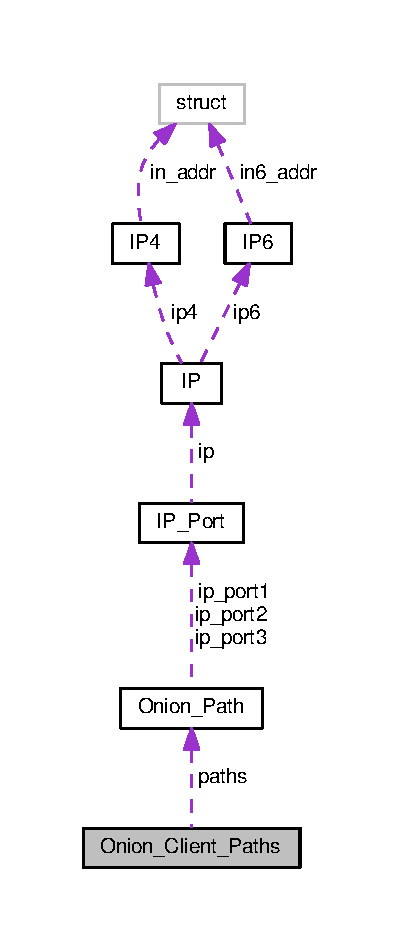
\includegraphics[width=192pt]{struct_onion___client___paths__coll__graph}
\end{center}
\end{figure}
\subsection*{Data Fields}
\begin{DoxyCompactItemize}
\item 
\hypertarget{struct_onion___client___paths_afaa8c1f23d89bd5acee1f956e8872061}{\hyperlink{struct_onion___path}{Onion\+\_\+\+Path} {\bfseries paths} \mbox{[}N\+U\+M\+B\+E\+R\+\_\+\+O\+N\+I\+O\+N\+\_\+\+P\+A\+T\+H\+S\mbox{]}}\label{struct_onion___client___paths_afaa8c1f23d89bd5acee1f956e8872061}

\item 
\hypertarget{struct_onion___client___paths_afbee813e09086f6993c94cdaafe2ae36}{uint64\+\_\+t {\bfseries last\+\_\+path\+\_\+success} \mbox{[}N\+U\+M\+B\+E\+R\+\_\+\+O\+N\+I\+O\+N\+\_\+\+P\+A\+T\+H\+S\mbox{]}}\label{struct_onion___client___paths_afbee813e09086f6993c94cdaafe2ae36}

\item 
\hypertarget{struct_onion___client___paths_a3e3d1429ce10f2adad7b1c02df8f5417}{uint64\+\_\+t {\bfseries last\+\_\+path\+\_\+used} \mbox{[}N\+U\+M\+B\+E\+R\+\_\+\+O\+N\+I\+O\+N\+\_\+\+P\+A\+T\+H\+S\mbox{]}}\label{struct_onion___client___paths_a3e3d1429ce10f2adad7b1c02df8f5417}

\item 
\hypertarget{struct_onion___client___paths_abc272861ece76f9d9bac356f7297ce3e}{uint64\+\_\+t {\bfseries path\+\_\+creation\+\_\+time} \mbox{[}N\+U\+M\+B\+E\+R\+\_\+\+O\+N\+I\+O\+N\+\_\+\+P\+A\+T\+H\+S\mbox{]}}\label{struct_onion___client___paths_abc272861ece76f9d9bac356f7297ce3e}

\item 
\hypertarget{struct_onion___client___paths_a3a947792d864563f1c4d6984cc9c638a}{unsigned int {\bfseries last\+\_\+path\+\_\+used\+\_\+times} \mbox{[}N\+U\+M\+B\+E\+R\+\_\+\+O\+N\+I\+O\+N\+\_\+\+P\+A\+T\+H\+S\mbox{]}}\label{struct_onion___client___paths_a3a947792d864563f1c4d6984cc9c638a}

\end{DoxyCompactItemize}


\subsection{Detailed Description}


Definition at line 76 of file onion\+\_\+client.\+h.



The documentation for this struct was generated from the following file\+:\begin{DoxyCompactItemize}
\item 
toxcore/onion\+\_\+client.\+h\end{DoxyCompactItemize}

\hypertarget{struct_onion___friend}{\section{Onion\+\_\+\+Friend Struct Reference}
\label{struct_onion___friend}\index{Onion\+\_\+\+Friend@{Onion\+\_\+\+Friend}}
}


Collaboration diagram for Onion\+\_\+\+Friend\+:\nopagebreak
\begin{figure}[H]
\begin{center}
\leavevmode
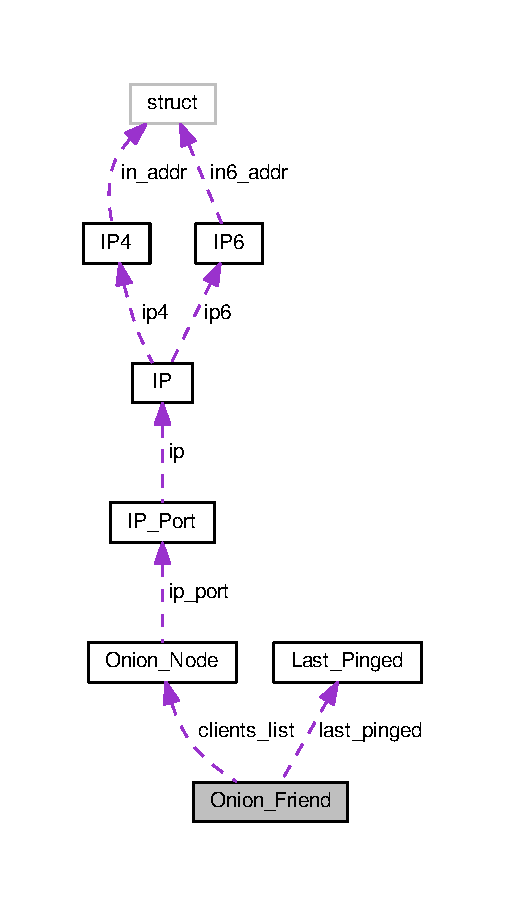
\includegraphics[width=243pt]{struct_onion___friend__coll__graph}
\end{center}
\end{figure}
\subsection*{Data Fields}
\begin{DoxyCompactItemize}
\item 
\hypertarget{struct_onion___friend_ade818037fd6c985038ff29656089758d}{uint8\+\_\+t {\bfseries status}}\label{struct_onion___friend_ade818037fd6c985038ff29656089758d}

\item 
\hypertarget{struct_onion___friend_a6e539a068fed61fab47b62f467c1d208}{uint8\+\_\+t {\bfseries is\+\_\+online}}\label{struct_onion___friend_a6e539a068fed61fab47b62f467c1d208}

\item 
\hypertarget{struct_onion___friend_a1b66769a2b6f8e5c7306ffcfb7ac0956}{uint8\+\_\+t {\bfseries know\+\_\+dht\+\_\+public\+\_\+key}}\label{struct_onion___friend_a1b66769a2b6f8e5c7306ffcfb7ac0956}

\item 
\hypertarget{struct_onion___friend_ab2ecaa07625ad0ed5e07d3a1f0dcc939}{uint8\+\_\+t {\bfseries dht\+\_\+public\+\_\+key} \mbox{[}crypto\+\_\+box\+\_\+\+P\+U\+B\+L\+I\+C\+K\+E\+Y\+B\+Y\+T\+E\+S\mbox{]}}\label{struct_onion___friend_ab2ecaa07625ad0ed5e07d3a1f0dcc939}

\item 
\hypertarget{struct_onion___friend_a996dcaefa2a5954a199e2beb584c1feb}{uint8\+\_\+t {\bfseries real\+\_\+public\+\_\+key} \mbox{[}crypto\+\_\+box\+\_\+\+P\+U\+B\+L\+I\+C\+K\+E\+Y\+B\+Y\+T\+E\+S\mbox{]}}\label{struct_onion___friend_a996dcaefa2a5954a199e2beb584c1feb}

\item 
\hypertarget{struct_onion___friend_a6797ac2f59ba5ef59a8a70cd6515ca25}{\hyperlink{struct_onion___node}{Onion\+\_\+\+Node} {\bfseries clients\+\_\+list} \mbox{[}M\+A\+X\+\_\+\+O\+N\+I\+O\+N\+\_\+\+C\+L\+I\+E\+N\+T\+S\mbox{]}}\label{struct_onion___friend_a6797ac2f59ba5ef59a8a70cd6515ca25}

\item 
\hypertarget{struct_onion___friend_afc342de3f1533c0adfd762a6fd0d20ab}{uint8\+\_\+t {\bfseries temp\+\_\+public\+\_\+key} \mbox{[}crypto\+\_\+box\+\_\+\+P\+U\+B\+L\+I\+C\+K\+E\+Y\+B\+Y\+T\+E\+S\mbox{]}}\label{struct_onion___friend_afc342de3f1533c0adfd762a6fd0d20ab}

\item 
\hypertarget{struct_onion___friend_a6de303feb7b7892cc6a38228554b3e78}{uint8\+\_\+t {\bfseries temp\+\_\+secret\+\_\+key} \mbox{[}crypto\+\_\+box\+\_\+\+S\+E\+C\+R\+E\+T\+K\+E\+Y\+B\+Y\+T\+E\+S\mbox{]}}\label{struct_onion___friend_a6de303feb7b7892cc6a38228554b3e78}

\item 
\hypertarget{struct_onion___friend_ac83f72b06d86503ee29943ccbe7f1a7a}{uint64\+\_\+t {\bfseries last\+\_\+dht\+\_\+pk\+\_\+onion\+\_\+sent}}\label{struct_onion___friend_ac83f72b06d86503ee29943ccbe7f1a7a}

\item 
\hypertarget{struct_onion___friend_a412168e37e1bdf5545f814c9c487aaeb}{uint64\+\_\+t {\bfseries last\+\_\+dht\+\_\+pk\+\_\+dht\+\_\+sent}}\label{struct_onion___friend_a412168e37e1bdf5545f814c9c487aaeb}

\item 
\hypertarget{struct_onion___friend_afeea50a96c079a530de60cf6389ec1bd}{uint64\+\_\+t {\bfseries last\+\_\+noreplay}}\label{struct_onion___friend_afeea50a96c079a530de60cf6389ec1bd}

\item 
\hypertarget{struct_onion___friend_a7418e248decb1dc63d1e1c8960092c33}{uint64\+\_\+t {\bfseries last\+\_\+seen}}\label{struct_onion___friend_a7418e248decb1dc63d1e1c8960092c33}

\item 
\hypertarget{struct_onion___friend_a27015cced65360814a59652b662ef143}{\hyperlink{struct_last___pinged}{Last\+\_\+\+Pinged} {\bfseries last\+\_\+pinged} \mbox{[}M\+A\+X\+\_\+\+S\+T\+O\+R\+E\+D\+\_\+\+P\+I\+N\+G\+E\+D\+\_\+\+N\+O\+D\+E\+S\mbox{]}}\label{struct_onion___friend_a27015cced65360814a59652b662ef143}

\item 
\hypertarget{struct_onion___friend_a6e0a5214a3dffa151dd52dc4c230145b}{uint8\+\_\+t {\bfseries last\+\_\+pinged\+\_\+index}}\label{struct_onion___friend_a6e0a5214a3dffa151dd52dc4c230145b}

\item 
\hypertarget{struct_onion___friend_a62001c45ecd44d4c6321ca2358f4df5f}{int($\ast$ {\bfseries tcp\+\_\+relay\+\_\+node\+\_\+callback} )(void $\ast$object, uint32\+\_\+t number, \hyperlink{struct_i_p___port}{I\+P\+\_\+\+Port} ip\+\_\+port, const uint8\+\_\+t $\ast$public\+\_\+key)}\label{struct_onion___friend_a62001c45ecd44d4c6321ca2358f4df5f}

\item 
\hypertarget{struct_onion___friend_a0da74cebd5ec2859b1de5db74c0dc528}{void $\ast$ {\bfseries tcp\+\_\+relay\+\_\+node\+\_\+callback\+\_\+object}}\label{struct_onion___friend_a0da74cebd5ec2859b1de5db74c0dc528}

\item 
\hypertarget{struct_onion___friend_ab673fb84fe578fb5e7848f9f04c093cf}{uint32\+\_\+t {\bfseries tcp\+\_\+relay\+\_\+node\+\_\+callback\+\_\+number}}\label{struct_onion___friend_ab673fb84fe578fb5e7848f9f04c093cf}

\item 
\hypertarget{struct_onion___friend_ab0f780a41ece58bf84d8460e71cbdbb3}{void($\ast$ {\bfseries dht\+\_\+pk\+\_\+callback} )(void $\ast$data, int32\+\_\+t number, const uint8\+\_\+t $\ast$dht\+\_\+public\+\_\+key)}\label{struct_onion___friend_ab0f780a41ece58bf84d8460e71cbdbb3}

\item 
\hypertarget{struct_onion___friend_ab5d618d73b8d83fb07209433e7b448ee}{void $\ast$ {\bfseries dht\+\_\+pk\+\_\+callback\+\_\+object}}\label{struct_onion___friend_ab5d618d73b8d83fb07209433e7b448ee}

\item 
\hypertarget{struct_onion___friend_ab0413da421baacf312141b8ae3ec7762}{uint32\+\_\+t {\bfseries dht\+\_\+pk\+\_\+callback\+\_\+number}}\label{struct_onion___friend_ab0413da421baacf312141b8ae3ec7762}

\item 
\hypertarget{struct_onion___friend_a9b6e91b90249c9b72d98611ba5ed7176}{uint32\+\_\+t {\bfseries run\+\_\+count}}\label{struct_onion___friend_a9b6e91b90249c9b72d98611ba5ed7176}

\end{DoxyCompactItemize}


\subsection{Detailed Description}


Definition at line 90 of file onion\+\_\+client.\+h.



The documentation for this struct was generated from the following file\+:\begin{DoxyCompactItemize}
\item 
toxcore/onion\+\_\+client.\+h\end{DoxyCompactItemize}

\hypertarget{struct_onion___node}{\section{Onion\+\_\+\+Node Struct Reference}
\label{struct_onion___node}\index{Onion\+\_\+\+Node@{Onion\+\_\+\+Node}}
}


Collaboration diagram for Onion\+\_\+\+Node\+:
\nopagebreak
\begin{figure}[H]
\begin{center}
\leavevmode
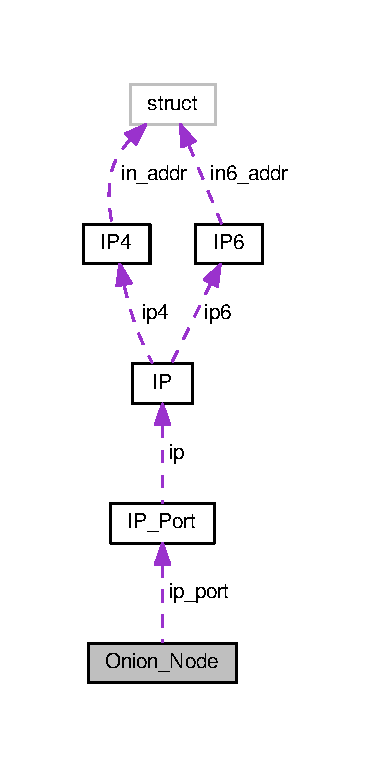
\includegraphics[width=178pt]{struct_onion___node__coll__graph}
\end{center}
\end{figure}
\subsection*{Data Fields}
\begin{DoxyCompactItemize}
\item 
\hypertarget{struct_onion___node_aaa806bb1136fb3d4b5d8d8970b596ff7}{uint8\+\_\+t {\bfseries public\+\_\+key} \mbox{[}crypto\+\_\+box\+\_\+\+P\+U\+B\+L\+I\+C\+K\+E\+Y\+B\+Y\+T\+E\+S\mbox{]}}\label{struct_onion___node_aaa806bb1136fb3d4b5d8d8970b596ff7}

\item 
\hypertarget{struct_onion___node_a86e2a5a56c0dd22df6e8b8a10e40f9e4}{\hyperlink{struct_i_p___port}{I\+P\+\_\+\+Port} {\bfseries ip\+\_\+port}}\label{struct_onion___node_a86e2a5a56c0dd22df6e8b8a10e40f9e4}

\item 
\hypertarget{struct_onion___node_aa21328f812472705a8d7bcee491bb54d}{uint8\+\_\+t {\bfseries ping\+\_\+id} \mbox{[}O\+N\+I\+O\+N\+\_\+\+P\+I\+N\+G\+\_\+\+I\+D\+\_\+\+S\+I\+Z\+E\mbox{]}}\label{struct_onion___node_aa21328f812472705a8d7bcee491bb54d}

\item 
\hypertarget{struct_onion___node_add8f6d39a7818b6d3ff0fca42a0aadf4}{uint8\+\_\+t {\bfseries data\+\_\+public\+\_\+key} \mbox{[}crypto\+\_\+box\+\_\+\+P\+U\+B\+L\+I\+C\+K\+E\+Y\+B\+Y\+T\+E\+S\mbox{]}}\label{struct_onion___node_add8f6d39a7818b6d3ff0fca42a0aadf4}

\item 
\hypertarget{struct_onion___node_ada3701a9ce02699f1b7e8f55a41379bf}{uint8\+\_\+t {\bfseries is\+\_\+stored}}\label{struct_onion___node_ada3701a9ce02699f1b7e8f55a41379bf}

\item 
\hypertarget{struct_onion___node_a465bef81f6478756e5443025b1f2ddfa}{uint64\+\_\+t {\bfseries timestamp}}\label{struct_onion___node_a465bef81f6478756e5443025b1f2ddfa}

\item 
\hypertarget{struct_onion___node_a4049204f6c392628d31be6c39f03e031}{uint64\+\_\+t {\bfseries last\+\_\+pinged}}\label{struct_onion___node_a4049204f6c392628d31be6c39f03e031}

\item 
\hypertarget{struct_onion___node_a75c3cb4fcbcf13c47379cc14737926d9}{uint32\+\_\+t {\bfseries path\+\_\+used}}\label{struct_onion___node_a75c3cb4fcbcf13c47379cc14737926d9}

\end{DoxyCompactItemize}


\subsection{Detailed Description}


Definition at line 62 of file onion\+\_\+client.\+h.



The documentation for this struct was generated from the following file\+:\begin{DoxyCompactItemize}
\item 
toxcore/onion\+\_\+client.\+h\end{DoxyCompactItemize}

\hypertarget{struct_onion___path}{\section{Onion\+\_\+\+Path Struct Reference}
\label{struct_onion___path}\index{Onion\+\_\+\+Path@{Onion\+\_\+\+Path}}
}


{\ttfamily \#include $<$onion.\+h$>$}



Collaboration diagram for Onion\+\_\+\+Path\+:
\nopagebreak
\begin{figure}[H]
\begin{center}
\leavevmode
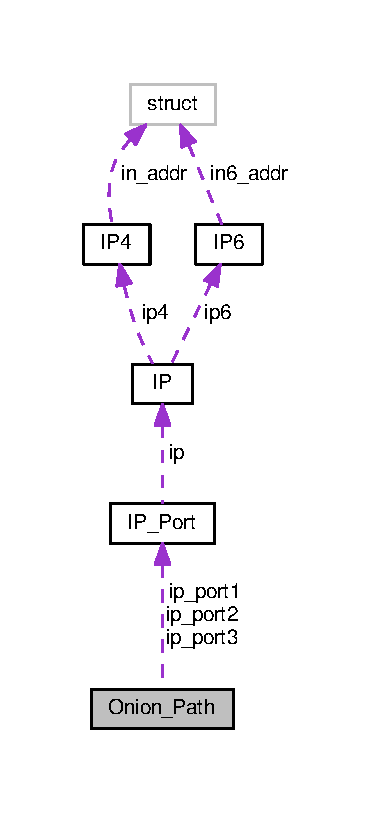
\includegraphics[width=178pt]{d2/d03/struct_onion___path__coll__graph}
\end{center}
\end{figure}
\subsection*{Data Fields}
\begin{DoxyCompactItemize}
\item 
uint8\+\_\+t \hyperlink{struct_onion___path_ac38c2cdd308cce10c53e276cb664c644}{shared\+\_\+key1} \mbox{[}crypto\+\_\+box\+\_\+\+B\+E\+F\+O\+R\+E\+N\+M\+B\+Y\+T\+E\+S\mbox{]}
\item 
uint8\+\_\+t \hyperlink{struct_onion___path_a677ff69e40fecc070cfe5ebe1f4ecb71}{shared\+\_\+key2} \mbox{[}crypto\+\_\+box\+\_\+\+B\+E\+F\+O\+R\+E\+N\+M\+B\+Y\+T\+E\+S\mbox{]}
\item 
uint8\+\_\+t \hyperlink{struct_onion___path_ab9b6dd504522fbbb77500ab7e5d27121}{shared\+\_\+key3} \mbox{[}crypto\+\_\+box\+\_\+\+B\+E\+F\+O\+R\+E\+N\+M\+B\+Y\+T\+E\+S\mbox{]}
\item 
uint8\+\_\+t \hyperlink{struct_onion___path_a203561e286f807c2f057fc6bce17e2d8}{public\+\_\+key1} \mbox{[}crypto\+\_\+box\+\_\+\+P\+U\+B\+L\+I\+C\+K\+E\+Y\+B\+Y\+T\+E\+S\mbox{]}
\item 
uint8\+\_\+t \hyperlink{struct_onion___path_adb351a6df6a87dbb748077bd8081270d}{public\+\_\+key2} \mbox{[}crypto\+\_\+box\+\_\+\+P\+U\+B\+L\+I\+C\+K\+E\+Y\+B\+Y\+T\+E\+S\mbox{]}
\item 
uint8\+\_\+t \hyperlink{struct_onion___path_a0fa442ed05e4279ea8bcb1d039724f2b}{public\+\_\+key3} \mbox{[}crypto\+\_\+box\+\_\+\+P\+U\+B\+L\+I\+C\+K\+E\+Y\+B\+Y\+T\+E\+S\mbox{]}
\item 
\hyperlink{struct_i_p___port}{I\+P\+\_\+\+Port} \hyperlink{struct_onion___path_ad7670c0a1a9d05b2a807a9c1a7950b79}{ip\+\_\+port1}
\item 
uint8\+\_\+t \hyperlink{struct_onion___path_a38f4e3f7780648cf74f808d7942113d8}{node\+\_\+public\+\_\+key1} \mbox{[}crypto\+\_\+box\+\_\+\+P\+U\+B\+L\+I\+C\+K\+E\+Y\+B\+Y\+T\+E\+S\mbox{]}
\item 
\hyperlink{struct_i_p___port}{I\+P\+\_\+\+Port} \hyperlink{struct_onion___path_adcf789584e4efc296bc6f915d3e2e9f9}{ip\+\_\+port2}
\item 
uint8\+\_\+t \hyperlink{struct_onion___path_adc5a9730c2f43085e83ece3257af154a}{node\+\_\+public\+\_\+key2} \mbox{[}crypto\+\_\+box\+\_\+\+P\+U\+B\+L\+I\+C\+K\+E\+Y\+B\+Y\+T\+E\+S\mbox{]}
\item 
\hyperlink{struct_i_p___port}{I\+P\+\_\+\+Port} \hyperlink{struct_onion___path_aef20a4d17084ae724f2e496f8f7a106a}{ip\+\_\+port3}
\item 
uint8\+\_\+t \hyperlink{struct_onion___path_a4725b29fc0349714fa0ab0938844cf19}{node\+\_\+public\+\_\+key3} \mbox{[}crypto\+\_\+box\+\_\+\+P\+U\+B\+L\+I\+C\+K\+E\+Y\+B\+Y\+T\+E\+S\mbox{]}
\item 
uint32\+\_\+t \hyperlink{struct_onion___path_a6d69f3ea5100411c3599020055b8b78c}{path\+\_\+num}
\end{DoxyCompactItemize}


\subsection{Detailed Description}


Definition at line 58 of file onion.\+h.



\subsection{Field Documentation}
\hypertarget{struct_onion___path_ad7670c0a1a9d05b2a807a9c1a7950b79}{\index{Onion\+\_\+\+Path@{Onion\+\_\+\+Path}!ip\+\_\+port1@{ip\+\_\+port1}}
\index{ip\+\_\+port1@{ip\+\_\+port1}!Onion\+\_\+\+Path@{Onion\+\_\+\+Path}}
\subsubsection[{ip\+\_\+port1}]{\setlength{\rightskip}{0pt plus 5cm}{\bf I\+P\+\_\+\+Port} ip\+\_\+port1}}\label{struct_onion___path_ad7670c0a1a9d05b2a807a9c1a7950b79}


Definition at line 67 of file onion.\+h.



Referenced by create\+\_\+onion\+\_\+path(), is\+\_\+path\+\_\+used(), onion\+\_\+path\+\_\+to\+\_\+nodes(), send\+\_\+announce\+\_\+request(), send\+\_\+data\+\_\+request(), send\+\_\+onion\+\_\+packet(), and send\+\_\+onion\+\_\+packet\+\_\+tcp\+\_\+udp().

\hypertarget{struct_onion___path_adcf789584e4efc296bc6f915d3e2e9f9}{\index{Onion\+\_\+\+Path@{Onion\+\_\+\+Path}!ip\+\_\+port2@{ip\+\_\+port2}}
\index{ip\+\_\+port2@{ip\+\_\+port2}!Onion\+\_\+\+Path@{Onion\+\_\+\+Path}}
\subsubsection[{ip\+\_\+port2}]{\setlength{\rightskip}{0pt plus 5cm}{\bf I\+P\+\_\+\+Port} ip\+\_\+port2}}\label{struct_onion___path_adcf789584e4efc296bc6f915d3e2e9f9}


Definition at line 70 of file onion.\+h.



Referenced by create\+\_\+onion\+\_\+packet(), create\+\_\+onion\+\_\+packet\+\_\+tcp(), create\+\_\+onion\+\_\+path(), and onion\+\_\+path\+\_\+to\+\_\+nodes().

\hypertarget{struct_onion___path_aef20a4d17084ae724f2e496f8f7a106a}{\index{Onion\+\_\+\+Path@{Onion\+\_\+\+Path}!ip\+\_\+port3@{ip\+\_\+port3}}
\index{ip\+\_\+port3@{ip\+\_\+port3}!Onion\+\_\+\+Path@{Onion\+\_\+\+Path}}
\subsubsection[{ip\+\_\+port3}]{\setlength{\rightskip}{0pt plus 5cm}{\bf I\+P\+\_\+\+Port} ip\+\_\+port3}}\label{struct_onion___path_aef20a4d17084ae724f2e496f8f7a106a}


Definition at line 73 of file onion.\+h.



Referenced by create\+\_\+onion\+\_\+packet(), create\+\_\+onion\+\_\+packet\+\_\+tcp(), create\+\_\+onion\+\_\+path(), and onion\+\_\+path\+\_\+to\+\_\+nodes().

\hypertarget{struct_onion___path_a38f4e3f7780648cf74f808d7942113d8}{\index{Onion\+\_\+\+Path@{Onion\+\_\+\+Path}!node\+\_\+public\+\_\+key1@{node\+\_\+public\+\_\+key1}}
\index{node\+\_\+public\+\_\+key1@{node\+\_\+public\+\_\+key1}!Onion\+\_\+\+Path@{Onion\+\_\+\+Path}}
\subsubsection[{node\+\_\+public\+\_\+key1}]{\setlength{\rightskip}{0pt plus 5cm}uint8\+\_\+t node\+\_\+public\+\_\+key1\mbox{[}crypto\+\_\+box\+\_\+\+P\+U\+B\+L\+I\+C\+K\+E\+Y\+B\+Y\+T\+E\+S\mbox{]}}}\label{struct_onion___path_a38f4e3f7780648cf74f808d7942113d8}


Definition at line 68 of file onion.\+h.



Referenced by create\+\_\+onion\+\_\+path(), and onion\+\_\+path\+\_\+to\+\_\+nodes().

\hypertarget{struct_onion___path_adc5a9730c2f43085e83ece3257af154a}{\index{Onion\+\_\+\+Path@{Onion\+\_\+\+Path}!node\+\_\+public\+\_\+key2@{node\+\_\+public\+\_\+key2}}
\index{node\+\_\+public\+\_\+key2@{node\+\_\+public\+\_\+key2}!Onion\+\_\+\+Path@{Onion\+\_\+\+Path}}
\subsubsection[{node\+\_\+public\+\_\+key2}]{\setlength{\rightskip}{0pt plus 5cm}uint8\+\_\+t node\+\_\+public\+\_\+key2\mbox{[}crypto\+\_\+box\+\_\+\+P\+U\+B\+L\+I\+C\+K\+E\+Y\+B\+Y\+T\+E\+S\mbox{]}}}\label{struct_onion___path_adc5a9730c2f43085e83ece3257af154a}


Definition at line 71 of file onion.\+h.



Referenced by create\+\_\+onion\+\_\+path(), and onion\+\_\+path\+\_\+to\+\_\+nodes().

\hypertarget{struct_onion___path_a4725b29fc0349714fa0ab0938844cf19}{\index{Onion\+\_\+\+Path@{Onion\+\_\+\+Path}!node\+\_\+public\+\_\+key3@{node\+\_\+public\+\_\+key3}}
\index{node\+\_\+public\+\_\+key3@{node\+\_\+public\+\_\+key3}!Onion\+\_\+\+Path@{Onion\+\_\+\+Path}}
\subsubsection[{node\+\_\+public\+\_\+key3}]{\setlength{\rightskip}{0pt plus 5cm}uint8\+\_\+t node\+\_\+public\+\_\+key3\mbox{[}crypto\+\_\+box\+\_\+\+P\+U\+B\+L\+I\+C\+K\+E\+Y\+B\+Y\+T\+E\+S\mbox{]}}}\label{struct_onion___path_a4725b29fc0349714fa0ab0938844cf19}


Definition at line 74 of file onion.\+h.



Referenced by create\+\_\+onion\+\_\+path(), and onion\+\_\+path\+\_\+to\+\_\+nodes().

\hypertarget{struct_onion___path_a6d69f3ea5100411c3599020055b8b78c}{\index{Onion\+\_\+\+Path@{Onion\+\_\+\+Path}!path\+\_\+num@{path\+\_\+num}}
\index{path\+\_\+num@{path\+\_\+num}!Onion\+\_\+\+Path@{Onion\+\_\+\+Path}}
\subsubsection[{path\+\_\+num}]{\setlength{\rightskip}{0pt plus 5cm}uint32\+\_\+t path\+\_\+num}}\label{struct_onion___path_a6d69f3ea5100411c3599020055b8b78c}


Definition at line 76 of file onion.\+h.



Referenced by client\+\_\+send\+\_\+announce\+\_\+request(), path\+\_\+exists(), random\+\_\+path(), and set\+\_\+path\+\_\+timeouts().

\hypertarget{struct_onion___path_a203561e286f807c2f057fc6bce17e2d8}{\index{Onion\+\_\+\+Path@{Onion\+\_\+\+Path}!public\+\_\+key1@{public\+\_\+key1}}
\index{public\+\_\+key1@{public\+\_\+key1}!Onion\+\_\+\+Path@{Onion\+\_\+\+Path}}
\subsubsection[{public\+\_\+key1}]{\setlength{\rightskip}{0pt plus 5cm}uint8\+\_\+t public\+\_\+key1\mbox{[}crypto\+\_\+box\+\_\+\+P\+U\+B\+L\+I\+C\+K\+E\+Y\+B\+Y\+T\+E\+S\mbox{]}}}\label{struct_onion___path_a203561e286f807c2f057fc6bce17e2d8}


Definition at line 63 of file onion.\+h.



Referenced by create\+\_\+onion\+\_\+packet(), and create\+\_\+onion\+\_\+path().

\hypertarget{struct_onion___path_adb351a6df6a87dbb748077bd8081270d}{\index{Onion\+\_\+\+Path@{Onion\+\_\+\+Path}!public\+\_\+key2@{public\+\_\+key2}}
\index{public\+\_\+key2@{public\+\_\+key2}!Onion\+\_\+\+Path@{Onion\+\_\+\+Path}}
\subsubsection[{public\+\_\+key2}]{\setlength{\rightskip}{0pt plus 5cm}uint8\+\_\+t public\+\_\+key2\mbox{[}crypto\+\_\+box\+\_\+\+P\+U\+B\+L\+I\+C\+K\+E\+Y\+B\+Y\+T\+E\+S\mbox{]}}}\label{struct_onion___path_adb351a6df6a87dbb748077bd8081270d}


Definition at line 64 of file onion.\+h.



Referenced by create\+\_\+onion\+\_\+packet(), create\+\_\+onion\+\_\+packet\+\_\+tcp(), and create\+\_\+onion\+\_\+path().

\hypertarget{struct_onion___path_a0fa442ed05e4279ea8bcb1d039724f2b}{\index{Onion\+\_\+\+Path@{Onion\+\_\+\+Path}!public\+\_\+key3@{public\+\_\+key3}}
\index{public\+\_\+key3@{public\+\_\+key3}!Onion\+\_\+\+Path@{Onion\+\_\+\+Path}}
\subsubsection[{public\+\_\+key3}]{\setlength{\rightskip}{0pt plus 5cm}uint8\+\_\+t public\+\_\+key3\mbox{[}crypto\+\_\+box\+\_\+\+P\+U\+B\+L\+I\+C\+K\+E\+Y\+B\+Y\+T\+E\+S\mbox{]}}}\label{struct_onion___path_a0fa442ed05e4279ea8bcb1d039724f2b}


Definition at line 65 of file onion.\+h.



Referenced by create\+\_\+onion\+\_\+packet(), create\+\_\+onion\+\_\+packet\+\_\+tcp(), and create\+\_\+onion\+\_\+path().

\hypertarget{struct_onion___path_ac38c2cdd308cce10c53e276cb664c644}{\index{Onion\+\_\+\+Path@{Onion\+\_\+\+Path}!shared\+\_\+key1@{shared\+\_\+key1}}
\index{shared\+\_\+key1@{shared\+\_\+key1}!Onion\+\_\+\+Path@{Onion\+\_\+\+Path}}
\subsubsection[{shared\+\_\+key1}]{\setlength{\rightskip}{0pt plus 5cm}uint8\+\_\+t shared\+\_\+key1\mbox{[}crypto\+\_\+box\+\_\+\+B\+E\+F\+O\+R\+E\+N\+M\+B\+Y\+T\+E\+S\mbox{]}}}\label{struct_onion___path_ac38c2cdd308cce10c53e276cb664c644}


Definition at line 59 of file onion.\+h.



Referenced by create\+\_\+onion\+\_\+packet(), and create\+\_\+onion\+\_\+path().

\hypertarget{struct_onion___path_a677ff69e40fecc070cfe5ebe1f4ecb71}{\index{Onion\+\_\+\+Path@{Onion\+\_\+\+Path}!shared\+\_\+key2@{shared\+\_\+key2}}
\index{shared\+\_\+key2@{shared\+\_\+key2}!Onion\+\_\+\+Path@{Onion\+\_\+\+Path}}
\subsubsection[{shared\+\_\+key2}]{\setlength{\rightskip}{0pt plus 5cm}uint8\+\_\+t shared\+\_\+key2\mbox{[}crypto\+\_\+box\+\_\+\+B\+E\+F\+O\+R\+E\+N\+M\+B\+Y\+T\+E\+S\mbox{]}}}\label{struct_onion___path_a677ff69e40fecc070cfe5ebe1f4ecb71}


Definition at line 60 of file onion.\+h.



Referenced by create\+\_\+onion\+\_\+packet(), create\+\_\+onion\+\_\+packet\+\_\+tcp(), and create\+\_\+onion\+\_\+path().

\hypertarget{struct_onion___path_ab9b6dd504522fbbb77500ab7e5d27121}{\index{Onion\+\_\+\+Path@{Onion\+\_\+\+Path}!shared\+\_\+key3@{shared\+\_\+key3}}
\index{shared\+\_\+key3@{shared\+\_\+key3}!Onion\+\_\+\+Path@{Onion\+\_\+\+Path}}
\subsubsection[{shared\+\_\+key3}]{\setlength{\rightskip}{0pt plus 5cm}uint8\+\_\+t shared\+\_\+key3\mbox{[}crypto\+\_\+box\+\_\+\+B\+E\+F\+O\+R\+E\+N\+M\+B\+Y\+T\+E\+S\mbox{]}}}\label{struct_onion___path_ab9b6dd504522fbbb77500ab7e5d27121}


Definition at line 61 of file onion.\+h.



Referenced by create\+\_\+onion\+\_\+packet(), create\+\_\+onion\+\_\+packet\+\_\+tcp(), and create\+\_\+onion\+\_\+path().



The documentation for this struct was generated from the following file\+:\begin{DoxyCompactItemize}
\item 
toxcore/\hyperlink{onion_8h}{onion.\+h}\end{DoxyCompactItemize}

\hypertarget{struct_onions}{\section{Onions Struct Reference}
\label{struct_onions}\index{Onions@{Onions}}
}


Collaboration diagram for Onions\+:
\nopagebreak
\begin{figure}[H]
\begin{center}
\leavevmode
\includegraphics[width=350pt]{struct_onions__coll__graph}
\end{center}
\end{figure}
\subsection*{Data Fields}
\begin{DoxyCompactItemize}
\item 
\hypertarget{struct_onions_a66fb4bf67c711a5ed3e7bbecec7fde30}{\hyperlink{struct_onion}{Onion} $\ast$ {\bfseries onion}}\label{struct_onions_a66fb4bf67c711a5ed3e7bbecec7fde30}

\item 
\hypertarget{struct_onions_a3a345721fb6be385f4b4519679a4609f}{\hyperlink{struct_onion___announce}{Onion\+\_\+\+Announce} $\ast$ {\bfseries onion\+\_\+a}}\label{struct_onions_a3a345721fb6be385f4b4519679a4609f}

\item 
\hypertarget{struct_onions_ae202b81f9a2c2fa80fd310a0996795fc}{\hyperlink{struct_onion___client}{Onion\+\_\+\+Client} $\ast$ {\bfseries onion\+\_\+c}}\label{struct_onions_ae202b81f9a2c2fa80fd310a0996795fc}

\end{DoxyCompactItemize}


\subsection{Detailed Description}


Definition at line 263 of file onion\+\_\+test.\+c.



The documentation for this struct was generated from the following file\+:\begin{DoxyCompactItemize}
\item 
auto\+\_\+tests/onion\+\_\+test.\+c\end{DoxyCompactItemize}

\hypertarget{struct_packet___data}{\section{Packet\+\_\+\+Data Struct Reference}
\label{struct_packet___data}\index{Packet\+\_\+\+Data@{Packet\+\_\+\+Data}}
}


{\ttfamily \#include $<$net\+\_\+crypto.\+h$>$}

\subsection*{Data Fields}
\begin{DoxyCompactItemize}
\item 
uint64\+\_\+t \hyperlink{struct_packet___data_ae6e5e2c139451ff48ec8dbba5d21bb50}{sent\+\_\+time}
\item 
uint16\+\_\+t \hyperlink{struct_packet___data_a1892eba2086d12ac2b09005aeb09ea3b}{length}
\item 
uint8\+\_\+t \hyperlink{struct_packet___data_ab895a6b34c217017925a6aea69c78c09}{data} \mbox{[}\hyperlink{net__crypto_8h_a1b6e5122f9fdc5ef548ccf920f0c246e}{M\+A\+X\+\_\+\+C\+R\+Y\+P\+T\+O\+\_\+\+D\+A\+T\+A\+\_\+\+S\+I\+Z\+E}\mbox{]}
\end{DoxyCompactItemize}


\subsection{Detailed Description}


Definition at line 88 of file net\+\_\+crypto.\+h.



\subsection{Field Documentation}
\hypertarget{struct_packet___data_ab895a6b34c217017925a6aea69c78c09}{\index{Packet\+\_\+\+Data@{Packet\+\_\+\+Data}!data@{data}}
\index{data@{data}!Packet\+\_\+\+Data@{Packet\+\_\+\+Data}}
\subsubsection[{data}]{\setlength{\rightskip}{0pt plus 5cm}uint8\+\_\+t data\mbox{[}{\bf M\+A\+X\+\_\+\+C\+R\+Y\+P\+T\+O\+\_\+\+D\+A\+T\+A\+\_\+\+S\+I\+Z\+E}\mbox{]}}}\label{struct_packet___data_ab895a6b34c217017925a6aea69c78c09}


Definition at line 91 of file net\+\_\+crypto.\+h.



Referenced by handle\+\_\+data\+\_\+packet\+\_\+helper(), reset\+\_\+max\+\_\+speed\+\_\+reached(), send\+\_\+lossless\+\_\+packet(), and send\+\_\+requested\+\_\+packets().

\hypertarget{struct_packet___data_a1892eba2086d12ac2b09005aeb09ea3b}{\index{Packet\+\_\+\+Data@{Packet\+\_\+\+Data}!length@{length}}
\index{length@{length}!Packet\+\_\+\+Data@{Packet\+\_\+\+Data}}
\subsubsection[{length}]{\setlength{\rightskip}{0pt plus 5cm}uint16\+\_\+t length}}\label{struct_packet___data_a1892eba2086d12ac2b09005aeb09ea3b}


Definition at line 90 of file net\+\_\+crypto.\+h.



Referenced by handle\+\_\+data\+\_\+packet\+\_\+helper(), reset\+\_\+max\+\_\+speed\+\_\+reached(), send\+\_\+lossless\+\_\+packet(), and send\+\_\+requested\+\_\+packets().

\hypertarget{struct_packet___data_ae6e5e2c139451ff48ec8dbba5d21bb50}{\index{Packet\+\_\+\+Data@{Packet\+\_\+\+Data}!sent\+\_\+time@{sent\+\_\+time}}
\index{sent\+\_\+time@{sent\+\_\+time}!Packet\+\_\+\+Data@{Packet\+\_\+\+Data}}
\subsubsection[{sent\+\_\+time}]{\setlength{\rightskip}{0pt plus 5cm}uint64\+\_\+t sent\+\_\+time}}\label{struct_packet___data_ae6e5e2c139451ff48ec8dbba5d21bb50}


Definition at line 89 of file net\+\_\+crypto.\+h.



Referenced by handle\+\_\+data\+\_\+packet\+\_\+helper(), handle\+\_\+request\+\_\+packet(), reset\+\_\+max\+\_\+speed\+\_\+reached(), send\+\_\+lossless\+\_\+packet(), and send\+\_\+requested\+\_\+packets().



The documentation for this struct was generated from the following file\+:\begin{DoxyCompactItemize}
\item 
toxcore/\hyperlink{net__crypto_8h}{net\+\_\+crypto.\+h}\end{DoxyCompactItemize}

\hypertarget{struct_packet___handles}{\section{Packet\+\_\+\+Handles Struct Reference}
\label{struct_packet___handles}\index{Packet\+\_\+\+Handles@{Packet\+\_\+\+Handles}}
}


{\ttfamily \#include $<$network.\+h$>$}



Collaboration diagram for Packet\+\_\+\+Handles\+:
\nopagebreak
\begin{figure}[H]
\begin{center}
\leavevmode
\includegraphics[width=185pt]{d4/d19/struct_packet___handles__coll__graph}
\end{center}
\end{figure}
\subsection*{Data Fields}
\begin{DoxyCompactItemize}
\item 
\hyperlink{network_8h_a01fb3f0e3fd19ed8eefe335b64934156}{packet\+\_\+handler\+\_\+callback} \hyperlink{struct_packet___handles_a197979c60c06b39ac717b08f5091dd0e}{function}
\item 
void $\ast$ \hyperlink{struct_packet___handles_a077376d12464f945e2414d5499c79b3f}{object}
\end{DoxyCompactItemize}


\subsection{Detailed Description}


Definition at line 291 of file network.\+h.



\subsection{Field Documentation}
\hypertarget{struct_packet___handles_a197979c60c06b39ac717b08f5091dd0e}{\index{Packet\+\_\+\+Handles@{Packet\+\_\+\+Handles}!function@{function}}
\index{function@{function}!Packet\+\_\+\+Handles@{Packet\+\_\+\+Handles}}
\subsubsection[{function}]{\setlength{\rightskip}{0pt plus 5cm}{\bf packet\+\_\+handler\+\_\+callback} function}}\label{struct_packet___handles_a197979c60c06b39ac717b08f5091dd0e}


Definition at line 292 of file network.\+h.



Referenced by networking\+\_\+poll(), and networking\+\_\+registerhandler().

\hypertarget{struct_packet___handles_a077376d12464f945e2414d5499c79b3f}{\index{Packet\+\_\+\+Handles@{Packet\+\_\+\+Handles}!object@{object}}
\index{object@{object}!Packet\+\_\+\+Handles@{Packet\+\_\+\+Handles}}
\subsubsection[{object}]{\setlength{\rightskip}{0pt plus 5cm}void$\ast$ object}}\label{struct_packet___handles_a077376d12464f945e2414d5499c79b3f}


Definition at line 293 of file network.\+h.



Referenced by networking\+\_\+poll(), and networking\+\_\+registerhandler().



The documentation for this struct was generated from the following file\+:\begin{DoxyCompactItemize}
\item 
toxcore/\hyperlink{network_8h}{network.\+h}\end{DoxyCompactItemize}

\hypertarget{struct_packets___array}{\section{Packets\+\_\+\+Array Struct Reference}
\label{struct_packets___array}\index{Packets\+\_\+\+Array@{Packets\+\_\+\+Array}}
}


{\ttfamily \#include $<$net\+\_\+crypto.\+h$>$}



Collaboration diagram for Packets\+\_\+\+Array\+:
\nopagebreak
\begin{figure}[H]
\begin{center}
\leavevmode
\includegraphics[width=161pt]{d9/d97/struct_packets___array__coll__graph}
\end{center}
\end{figure}
\subsection*{Data Fields}
\begin{DoxyCompactItemize}
\item 
\hyperlink{struct_packet___data}{Packet\+\_\+\+Data} $\ast$ \hyperlink{struct_packets___array_ae9d4e6271fdb80e86ebb3e846fcd709c}{buffer} \mbox{[}\hyperlink{net__crypto_8h_ac73cf1eb0a938f0962ddc607945636f4}{C\+R\+Y\+P\+T\+O\+\_\+\+P\+A\+C\+K\+E\+T\+\_\+\+B\+U\+F\+F\+E\+R\+\_\+\+S\+I\+Z\+E}\mbox{]}
\item 
uint32\+\_\+t \hyperlink{struct_packets___array_a85973b335814248c05f63543876b348e}{buffer\+\_\+start}
\item 
uint32\+\_\+t \hyperlink{struct_packets___array_a66d710e0093872b26ee80118c1a85d99}{buffer\+\_\+end}
\end{DoxyCompactItemize}


\subsection{Detailed Description}


Definition at line 94 of file net\+\_\+crypto.\+h.



\subsection{Field Documentation}
\hypertarget{struct_packets___array_ae9d4e6271fdb80e86ebb3e846fcd709c}{\index{Packets\+\_\+\+Array@{Packets\+\_\+\+Array}!buffer@{buffer}}
\index{buffer@{buffer}!Packets\+\_\+\+Array@{Packets\+\_\+\+Array}}
\subsubsection[{buffer}]{\setlength{\rightskip}{0pt plus 5cm}{\bf Packet\+\_\+\+Data}$\ast$ buffer\mbox{[}{\bf C\+R\+Y\+P\+T\+O\+\_\+\+P\+A\+C\+K\+E\+T\+\_\+\+B\+U\+F\+F\+E\+R\+\_\+\+S\+I\+Z\+E}\mbox{]}}}\label{struct_packets___array_ae9d4e6271fdb80e86ebb3e846fcd709c}


Definition at line 95 of file net\+\_\+crypto.\+h.



Referenced by add\+\_\+data\+\_\+end\+\_\+of\+\_\+buffer(), add\+\_\+data\+\_\+to\+\_\+buffer(), clear\+\_\+buffer(), clear\+\_\+buffer\+\_\+until(), generate\+\_\+request\+\_\+packet(), get\+\_\+data\+\_\+pointer(), handle\+\_\+request\+\_\+packet(), and read\+\_\+data\+\_\+beg\+\_\+buffer().

\hypertarget{struct_packets___array_a66d710e0093872b26ee80118c1a85d99}{\index{Packets\+\_\+\+Array@{Packets\+\_\+\+Array}!buffer\+\_\+end@{buffer\+\_\+end}}
\index{buffer\+\_\+end@{buffer\+\_\+end}!Packets\+\_\+\+Array@{Packets\+\_\+\+Array}}
\subsubsection[{buffer\+\_\+end}]{\setlength{\rightskip}{0pt plus 5cm}uint32\+\_\+t buffer\+\_\+end}}\label{struct_packets___array_a66d710e0093872b26ee80118c1a85d99}


Definition at line 97 of file net\+\_\+crypto.\+h.



Referenced by add\+\_\+data\+\_\+end\+\_\+of\+\_\+buffer(), add\+\_\+data\+\_\+to\+\_\+buffer(), clear\+\_\+buffer(), clear\+\_\+buffer\+\_\+until(), cryptpacket\+\_\+received(), generate\+\_\+request\+\_\+packet(), get\+\_\+data\+\_\+pointer(), handle\+\_\+request\+\_\+packet(), num\+\_\+packets\+\_\+array(), read\+\_\+data\+\_\+beg\+\_\+buffer(), reset\+\_\+max\+\_\+speed\+\_\+reached(), send\+\_\+kill\+\_\+packet(), send\+\_\+lossy\+\_\+cryptpacket(), send\+\_\+request\+\_\+packet(), and set\+\_\+buffer\+\_\+end().

\hypertarget{struct_packets___array_a85973b335814248c05f63543876b348e}{\index{Packets\+\_\+\+Array@{Packets\+\_\+\+Array}!buffer\+\_\+start@{buffer\+\_\+start}}
\index{buffer\+\_\+start@{buffer\+\_\+start}!Packets\+\_\+\+Array@{Packets\+\_\+\+Array}}
\subsubsection[{buffer\+\_\+start}]{\setlength{\rightskip}{0pt plus 5cm}uint32\+\_\+t buffer\+\_\+start}}\label{struct_packets___array_a85973b335814248c05f63543876b348e}


Definition at line 96 of file net\+\_\+crypto.\+h.



Referenced by add\+\_\+data\+\_\+to\+\_\+buffer(), clear\+\_\+buffer(), clear\+\_\+buffer\+\_\+until(), cryptpacket\+\_\+received(), generate\+\_\+request\+\_\+packet(), get\+\_\+data\+\_\+pointer(), handle\+\_\+data\+\_\+packet\+\_\+helper(), handle\+\_\+request\+\_\+packet(), num\+\_\+packets\+\_\+array(), read\+\_\+data\+\_\+beg\+\_\+buffer(), reset\+\_\+max\+\_\+speed\+\_\+reached(), send\+\_\+kill\+\_\+packet(), send\+\_\+lossless\+\_\+packet(), send\+\_\+lossy\+\_\+cryptpacket(), send\+\_\+request\+\_\+packet(), send\+\_\+requested\+\_\+packets(), and set\+\_\+buffer\+\_\+end().



The documentation for this struct was generated from the following file\+:\begin{DoxyCompactItemize}
\item 
toxcore/\hyperlink{net__crypto_8h}{net\+\_\+crypto.\+h}\end{DoxyCompactItemize}

\hypertarget{struct_p_i_n_g}{\section{P\+I\+N\+G Struct Reference}
\label{struct_p_i_n_g}\index{P\+I\+N\+G@{P\+I\+N\+G}}
}


Collaboration diagram for P\+I\+N\+G\+:\nopagebreak
\begin{figure}[H]
\begin{center}
\leavevmode
\includegraphics[width=350pt]{struct_p_i_n_g__coll__graph}
\end{center}
\end{figure}
\subsection*{Data Fields}
\begin{DoxyCompactItemize}
\item 
\hypertarget{struct_p_i_n_g_a8b3d6ce8745acc52695e252bdb1531b6}{\hyperlink{struct_d_h_t}{D\+H\+T} $\ast$ {\bfseries dht}}\label{struct_p_i_n_g_a8b3d6ce8745acc52695e252bdb1531b6}

\item 
\hypertarget{struct_p_i_n_g_afb64d37a183969be553d23416dc47a4b}{\hyperlink{struct_ping___array}{Ping\+\_\+\+Array} {\bfseries ping\+\_\+array}}\label{struct_p_i_n_g_afb64d37a183969be553d23416dc47a4b}

\item 
\hypertarget{struct_p_i_n_g_a285072fd4cc519802afa28bef4227c57}{\hyperlink{struct_node__format}{Node\+\_\+format} {\bfseries to\+\_\+ping} \mbox{[}M\+A\+X\+\_\+\+T\+O\+\_\+\+P\+I\+N\+G\mbox{]}}\label{struct_p_i_n_g_a285072fd4cc519802afa28bef4227c57}

\item 
\hypertarget{struct_p_i_n_g_afc22124d671081ed5b12fc2fa71801d3}{uint64\+\_\+t {\bfseries last\+\_\+to\+\_\+ping}}\label{struct_p_i_n_g_afc22124d671081ed5b12fc2fa71801d3}

\end{DoxyCompactItemize}


\subsection{Detailed Description}


Definition at line 48 of file ping.\+c.



The documentation for this struct was generated from the following file\+:\begin{DoxyCompactItemize}
\item 
toxcore/ping.\+c\end{DoxyCompactItemize}

\hypertarget{struct_ping___array}{\section{Ping\+\_\+\+Array Struct Reference}
\label{struct_ping___array}\index{Ping\+\_\+\+Array@{Ping\+\_\+\+Array}}
}


Collaboration diagram for Ping\+\_\+\+Array\+:\nopagebreak
\begin{figure}[H]
\begin{center}
\leavevmode
\includegraphics[width=173pt]{struct_ping___array__coll__graph}
\end{center}
\end{figure}
\subsection*{Data Fields}
\begin{DoxyCompactItemize}
\item 
\hypertarget{struct_ping___array_a313b705ae8f0db8c02b2847b315ca1b1}{\hyperlink{struct_ping___array___entry}{Ping\+\_\+\+Array\+\_\+\+Entry} $\ast$ {\bfseries entries}}\label{struct_ping___array_a313b705ae8f0db8c02b2847b315ca1b1}

\item 
\hypertarget{struct_ping___array_ab3011676335a878a2c94492a37a63c3f}{uint32\+\_\+t {\bfseries last\+\_\+deleted}}\label{struct_ping___array_ab3011676335a878a2c94492a37a63c3f}

\item 
\hypertarget{struct_ping___array_a812ff28187c193e9a813628c36257df8}{uint32\+\_\+t {\bfseries last\+\_\+added}}\label{struct_ping___array_a812ff28187c193e9a813628c36257df8}

\item 
\hypertarget{struct_ping___array_acdfd526bb392e1ee59a3c6c545891b48}{uint32\+\_\+t {\bfseries total\+\_\+size}}\label{struct_ping___array_acdfd526bb392e1ee59a3c6c545891b48}

\item 
\hypertarget{struct_ping___array_ab5627d8d8b095c198e2523c44ca380ac}{uint32\+\_\+t {\bfseries timeout}}\label{struct_ping___array_ab5627d8d8b095c198e2523c44ca380ac}

\end{DoxyCompactItemize}


\subsection{Detailed Description}


Definition at line 36 of file ping\+\_\+array.\+h.



The documentation for this struct was generated from the following file\+:\begin{DoxyCompactItemize}
\item 
toxcore/ping\+\_\+array.\+h\end{DoxyCompactItemize}

\hypertarget{struct_ping___array___entry}{\section{Ping\+\_\+\+Array\+\_\+\+Entry Struct Reference}
\label{struct_ping___array___entry}\index{Ping\+\_\+\+Array\+\_\+\+Entry@{Ping\+\_\+\+Array\+\_\+\+Entry}}
}
\subsection*{Data Fields}
\begin{DoxyCompactItemize}
\item 
\hypertarget{struct_ping___array___entry_a735984d41155bc1032e09bece8f8d66d}{void $\ast$ {\bfseries data}}\label{struct_ping___array___entry_a735984d41155bc1032e09bece8f8d66d}

\item 
\hypertarget{struct_ping___array___entry_aebb70c2aab3407a9f05334c47131a43b}{uint32\+\_\+t {\bfseries length}}\label{struct_ping___array___entry_aebb70c2aab3407a9f05334c47131a43b}

\item 
\hypertarget{struct_ping___array___entry_a5d34a8f2dfe25421b2b473a5fd37b0ed}{uint64\+\_\+t {\bfseries time}}\label{struct_ping___array___entry_a5d34a8f2dfe25421b2b473a5fd37b0ed}

\item 
\hypertarget{struct_ping___array___entry_acec02fbdff648ca71a6d8e5a0d63d634}{uint64\+\_\+t {\bfseries ping\+\_\+id}}\label{struct_ping___array___entry_acec02fbdff648ca71a6d8e5a0d63d634}

\end{DoxyCompactItemize}


\subsection{Detailed Description}


Definition at line 28 of file ping\+\_\+array.\+h.



The documentation for this struct was generated from the following file\+:\begin{DoxyCompactItemize}
\item 
toxcore/ping\+\_\+array.\+h\end{DoxyCompactItemize}

\hypertarget{struct_receipts}{\section{Receipts Struct Reference}
\label{struct_receipts}\index{Receipts@{Receipts}}
}


Collaboration diagram for Receipts\+:\nopagebreak
\begin{figure}[H]
\begin{center}
\leavevmode
\includegraphics[width=136pt]{struct_receipts__coll__graph}
\end{center}
\end{figure}
\subsection*{Data Fields}
\begin{DoxyCompactItemize}
\item 
\hypertarget{struct_receipts_a3110fa374a202ca37de05e1bb9c95f17}{uint32\+\_\+t {\bfseries packet\+\_\+num}}\label{struct_receipts_a3110fa374a202ca37de05e1bb9c95f17}

\item 
\hypertarget{struct_receipts_a8d62bc717240dc62a7c3595d7b2a75ff}{uint32\+\_\+t {\bfseries msg\+\_\+id}}\label{struct_receipts_a8d62bc717240dc62a7c3595d7b2a75ff}

\item 
\hypertarget{struct_receipts_a4cf1c9c7aa66ba420c540e3070555c89}{struct \hyperlink{struct_receipts}{Receipts} $\ast$ {\bfseries next}}\label{struct_receipts_a4cf1c9c7aa66ba420c540e3070555c89}

\end{DoxyCompactItemize}


\subsection{Detailed Description}


Definition at line 77 of file Messenger.\+h.



The documentation for this struct was generated from the following file\+:\begin{DoxyCompactItemize}
\item 
toxcore/Messenger.\+h\end{DoxyCompactItemize}

\hypertarget{struct_s_a_v_e_d___f_r_i_e_n_d}{\section{S\+A\+V\+E\+D\+\_\+\+F\+R\+I\+E\+N\+D Struct Reference}
\label{struct_s_a_v_e_d___f_r_i_e_n_d}\index{S\+A\+V\+E\+D\+\_\+\+F\+R\+I\+E\+N\+D@{S\+A\+V\+E\+D\+\_\+\+F\+R\+I\+E\+N\+D}}
}
\subsection*{Data Fields}
\begin{DoxyCompactItemize}
\item 
\hypertarget{struct_s_a_v_e_d___f_r_i_e_n_d_ade818037fd6c985038ff29656089758d}{uint8\+\_\+t {\bfseries status}}\label{struct_s_a_v_e_d___f_r_i_e_n_d_ade818037fd6c985038ff29656089758d}

\item 
\hypertarget{struct_s_a_v_e_d___f_r_i_e_n_d_ab42b4c90d81ac99b968c3edd1e21d706}{uint8\+\_\+t {\bfseries real\+\_\+pk} \mbox{[}crypto\+\_\+box\+\_\+\+P\+U\+B\+L\+I\+C\+K\+E\+Y\+B\+Y\+T\+E\+S\mbox{]}}\label{struct_s_a_v_e_d___f_r_i_e_n_d_ab42b4c90d81ac99b968c3edd1e21d706}

\item 
\hypertarget{struct_s_a_v_e_d___f_r_i_e_n_d_a30d0b669f0c53df867104ef9fc4ca5ac}{uint8\+\_\+t {\bfseries info} \mbox{[}S\+A\+V\+E\+D\+\_\+\+F\+R\+I\+E\+N\+D\+\_\+\+R\+E\+Q\+U\+E\+S\+T\+\_\+\+S\+I\+Z\+E\mbox{]}}\label{struct_s_a_v_e_d___f_r_i_e_n_d_a30d0b669f0c53df867104ef9fc4ca5ac}

\item 
\hypertarget{struct_s_a_v_e_d___f_r_i_e_n_d_ac0ae002db55ef8f8366de10ec005b65a}{uint16\+\_\+t {\bfseries info\+\_\+size}}\label{struct_s_a_v_e_d___f_r_i_e_n_d_ac0ae002db55ef8f8366de10ec005b65a}

\item 
\hypertarget{struct_s_a_v_e_d___f_r_i_e_n_d_a11b8cc6595eea79e65c978209278e683}{uint8\+\_\+t {\bfseries name} \mbox{[}M\+A\+X\+\_\+\+N\+A\+M\+E\+\_\+\+L\+E\+N\+G\+T\+H\mbox{]}}\label{struct_s_a_v_e_d___f_r_i_e_n_d_a11b8cc6595eea79e65c978209278e683}

\item 
\hypertarget{struct_s_a_v_e_d___f_r_i_e_n_d_a3573d7a906b26e9999cd74f2c4066601}{uint16\+\_\+t {\bfseries name\+\_\+length}}\label{struct_s_a_v_e_d___f_r_i_e_n_d_a3573d7a906b26e9999cd74f2c4066601}

\item 
\hypertarget{struct_s_a_v_e_d___f_r_i_e_n_d_a8f12612ac1191135a1a5b1cbcbc82852}{uint8\+\_\+t {\bfseries statusmessage} \mbox{[}M\+A\+X\+\_\+\+S\+T\+A\+T\+U\+S\+M\+E\+S\+S\+A\+G\+E\+\_\+\+L\+E\+N\+G\+T\+H\mbox{]}}\label{struct_s_a_v_e_d___f_r_i_e_n_d_a8f12612ac1191135a1a5b1cbcbc82852}

\item 
\hypertarget{struct_s_a_v_e_d___f_r_i_e_n_d_a43fe9dde52dc12e90933150eca91c0c3}{uint16\+\_\+t {\bfseries statusmessage\+\_\+length}}\label{struct_s_a_v_e_d___f_r_i_e_n_d_a43fe9dde52dc12e90933150eca91c0c3}

\item 
\hypertarget{struct_s_a_v_e_d___f_r_i_e_n_d_a6985227ceff68d0298d6ee9e09316945}{uint8\+\_\+t {\bfseries userstatus}}\label{struct_s_a_v_e_d___f_r_i_e_n_d_a6985227ceff68d0298d6ee9e09316945}

\item 
\hypertarget{struct_s_a_v_e_d___f_r_i_e_n_d_a0fae9801a4789a368f90125119e31f3f}{uint32\+\_\+t {\bfseries friendrequest\+\_\+nospam}}\label{struct_s_a_v_e_d___f_r_i_e_n_d_a0fae9801a4789a368f90125119e31f3f}

\item 
\hypertarget{struct_s_a_v_e_d___f_r_i_e_n_d_a8f99c48eb6b3ea472806495135ab6792}{uint64\+\_\+t {\bfseries last\+\_\+seen\+\_\+time}}\label{struct_s_a_v_e_d___f_r_i_e_n_d_a8f99c48eb6b3ea472806495135ab6792}

\end{DoxyCompactItemize}


\subsection{Detailed Description}


Definition at line 2433 of file Messenger.\+c.



The documentation for this struct was generated from the following file\+:\begin{DoxyCompactItemize}
\item 
toxcore/Messenger.\+c\end{DoxyCompactItemize}

\hypertarget{structsec___t_c_p__con}{\section{sec\+\_\+\+T\+C\+P\+\_\+con Struct Reference}
\label{structsec___t_c_p__con}\index{sec\+\_\+\+T\+C\+P\+\_\+con@{sec\+\_\+\+T\+C\+P\+\_\+con}}
}
\subsection*{Data Fields}
\begin{DoxyCompactItemize}
\item 
\hypertarget{structsec___t_c_p__con_a35b19d84fb632ca8ce5cab237f7089a5}{sock\+\_\+t {\bfseries sock}}\label{structsec___t_c_p__con_a35b19d84fb632ca8ce5cab237f7089a5}

\item 
\hypertarget{structsec___t_c_p__con_aaa806bb1136fb3d4b5d8d8970b596ff7}{uint8\+\_\+t {\bfseries public\+\_\+key} \mbox{[}crypto\+\_\+box\+\_\+\+P\+U\+B\+L\+I\+C\+K\+E\+Y\+B\+Y\+T\+E\+S\mbox{]}}\label{structsec___t_c_p__con_aaa806bb1136fb3d4b5d8d8970b596ff7}

\item 
\hypertarget{structsec___t_c_p__con_aae0467706f97aa3ef23e5dc9c3c199d7}{uint8\+\_\+t {\bfseries recv\+\_\+nonce} \mbox{[}crypto\+\_\+box\+\_\+\+N\+O\+N\+C\+E\+B\+Y\+T\+E\+S\mbox{]}}\label{structsec___t_c_p__con_aae0467706f97aa3ef23e5dc9c3c199d7}

\item 
\hypertarget{structsec___t_c_p__con_a9df0e00e8f493ed6cd1ff45e7da33c0d}{uint8\+\_\+t {\bfseries sent\+\_\+nonce} \mbox{[}crypto\+\_\+box\+\_\+\+N\+O\+N\+C\+E\+B\+Y\+T\+E\+S\mbox{]}}\label{structsec___t_c_p__con_a9df0e00e8f493ed6cd1ff45e7da33c0d}

\item 
\hypertarget{structsec___t_c_p__con_a81ead9fac55a0cedc30a96253a2c5119}{uint8\+\_\+t {\bfseries shared\+\_\+key} \mbox{[}crypto\+\_\+box\+\_\+\+B\+E\+F\+O\+R\+E\+N\+M\+B\+Y\+T\+E\+S\mbox{]}}\label{structsec___t_c_p__con_a81ead9fac55a0cedc30a96253a2c5119}

\end{DoxyCompactItemize}


\subsection{Detailed Description}


Definition at line 125 of file T\+C\+P\+\_\+test.\+c.



The documentation for this struct was generated from the following file\+:\begin{DoxyCompactItemize}
\item 
auto\+\_\+tests/T\+C\+P\+\_\+test.\+c\end{DoxyCompactItemize}

\hypertarget{struct_shared___keys}{\section{Shared\+\_\+\+Keys Struct Reference}
\label{struct_shared___keys}\index{Shared\+\_\+\+Keys@{Shared\+\_\+\+Keys}}
}


Collaboration diagram for Shared\+\_\+\+Keys\+:\nopagebreak
\begin{figure}[H]
\begin{center}
\leavevmode
\includegraphics[width=155pt]{struct_shared___keys__coll__graph}
\end{center}
\end{figure}
\subsection*{Data Fields}
\begin{DoxyCompactItemize}
\item 
\hypertarget{struct_shared___keys_a15077d043938aa92f7ee5278d0036f7f}{\begin{tabbing}
xx\=xx\=xx\=xx\=xx\=xx\=xx\=xx\=xx\=\kill
struct \{\\
\>uint8\_t {\bfseries public\_key} \mbox{[}crypto\_box\_PUBLICKEYBYTES\mbox{]}\\
\>uint8\_t {\bfseries shared\_key} \mbox{[}crypto\_box\_BEFORENMBYTES\mbox{]}\\
\>uint32\_t {\bfseries times\_requested}\\
\>uint8\_t {\bfseries stored}\\
\>uint64\_t {\bfseries time\_last\_requested}\\
\} {\bfseries keys} \mbox{[}256 $\ast$MAX\_KEYS\_PER\_SLOT\mbox{]}}\label{struct_shared___keys_a15077d043938aa92f7ee5278d0036f7f}
\\

\end{tabbing}\end{DoxyCompactItemize}


\subsection{Detailed Description}


Definition at line 180 of file D\+H\+T.\+h.



The documentation for this struct was generated from the following file\+:\begin{DoxyCompactItemize}
\item 
toxcore/D\+H\+T.\+h\end{DoxyCompactItemize}

\hypertarget{struct_t_c_p___client___connection}{\section{T\+C\+P\+\_\+\+Client\+\_\+\+Connection Struct Reference}
\label{struct_t_c_p___client___connection}\index{T\+C\+P\+\_\+\+Client\+\_\+\+Connection@{T\+C\+P\+\_\+\+Client\+\_\+\+Connection}}
}


Collaboration diagram for T\+C\+P\+\_\+\+Client\+\_\+\+Connection\+:
\nopagebreak
\begin{figure}[H]
\begin{center}
\leavevmode
\includegraphics[width=350pt]{struct_t_c_p___client___connection__coll__graph}
\end{center}
\end{figure}
\subsection*{Data Fields}
\begin{DoxyCompactItemize}
\item 
\hypertarget{struct_t_c_p___client___connection_ade818037fd6c985038ff29656089758d}{uint8\+\_\+t {\bfseries status}}\label{struct_t_c_p___client___connection_ade818037fd6c985038ff29656089758d}

\item 
\hypertarget{struct_t_c_p___client___connection_a35b19d84fb632ca8ce5cab237f7089a5}{sock\+\_\+t {\bfseries sock}}\label{struct_t_c_p___client___connection_a35b19d84fb632ca8ce5cab237f7089a5}

\item 
\hypertarget{struct_t_c_p___client___connection_ae726df8bdc26380e5a6c3187a00d6881}{uint8\+\_\+t {\bfseries self\+\_\+public\+\_\+key} \mbox{[}crypto\+\_\+box\+\_\+\+P\+U\+B\+L\+I\+C\+K\+E\+Y\+B\+Y\+T\+E\+S\mbox{]}}\label{struct_t_c_p___client___connection_ae726df8bdc26380e5a6c3187a00d6881}

\item 
\hypertarget{struct_t_c_p___client___connection_aaa806bb1136fb3d4b5d8d8970b596ff7}{uint8\+\_\+t {\bfseries public\+\_\+key} \mbox{[}crypto\+\_\+box\+\_\+\+P\+U\+B\+L\+I\+C\+K\+E\+Y\+B\+Y\+T\+E\+S\mbox{]}}\label{struct_t_c_p___client___connection_aaa806bb1136fb3d4b5d8d8970b596ff7}

\item 
\hypertarget{struct_t_c_p___client___connection_a86e2a5a56c0dd22df6e8b8a10e40f9e4}{\hyperlink{struct_i_p___port}{I\+P\+\_\+\+Port} {\bfseries ip\+\_\+port}}\label{struct_t_c_p___client___connection_a86e2a5a56c0dd22df6e8b8a10e40f9e4}

\item 
\hypertarget{struct_t_c_p___client___connection_aa737023350cf47e63993e3b4dc9a7472}{\hyperlink{struct_t_c_p___proxy___info}{T\+C\+P\+\_\+\+Proxy\+\_\+\+Info} {\bfseries proxy\+\_\+info}}\label{struct_t_c_p___client___connection_aa737023350cf47e63993e3b4dc9a7472}

\item 
\hypertarget{struct_t_c_p___client___connection_aae0467706f97aa3ef23e5dc9c3c199d7}{uint8\+\_\+t {\bfseries recv\+\_\+nonce} \mbox{[}crypto\+\_\+box\+\_\+\+N\+O\+N\+C\+E\+B\+Y\+T\+E\+S\mbox{]}}\label{struct_t_c_p___client___connection_aae0467706f97aa3ef23e5dc9c3c199d7}

\item 
\hypertarget{struct_t_c_p___client___connection_a9df0e00e8f493ed6cd1ff45e7da33c0d}{uint8\+\_\+t {\bfseries sent\+\_\+nonce} \mbox{[}crypto\+\_\+box\+\_\+\+N\+O\+N\+C\+E\+B\+Y\+T\+E\+S\mbox{]}}\label{struct_t_c_p___client___connection_a9df0e00e8f493ed6cd1ff45e7da33c0d}

\item 
\hypertarget{struct_t_c_p___client___connection_a81ead9fac55a0cedc30a96253a2c5119}{uint8\+\_\+t {\bfseries shared\+\_\+key} \mbox{[}crypto\+\_\+box\+\_\+\+B\+E\+F\+O\+R\+E\+N\+M\+B\+Y\+T\+E\+S\mbox{]}}\label{struct_t_c_p___client___connection_a81ead9fac55a0cedc30a96253a2c5119}

\item 
\hypertarget{struct_t_c_p___client___connection_a1d1e3047af3c935db36ae7b2360aaec7}{uint16\+\_\+t {\bfseries next\+\_\+packet\+\_\+length}}\label{struct_t_c_p___client___connection_a1d1e3047af3c935db36ae7b2360aaec7}

\item 
\hypertarget{struct_t_c_p___client___connection_a6de303feb7b7892cc6a38228554b3e78}{uint8\+\_\+t {\bfseries temp\+\_\+secret\+\_\+key} \mbox{[}crypto\+\_\+box\+\_\+\+S\+E\+C\+R\+E\+T\+K\+E\+Y\+B\+Y\+T\+E\+S\mbox{]}}\label{struct_t_c_p___client___connection_a6de303feb7b7892cc6a38228554b3e78}

\item 
\hypertarget{struct_t_c_p___client___connection_af7b6d103d243e4267b112f6efe1573e2}{uint8\+\_\+t {\bfseries last\+\_\+packet} \mbox{[}2+M\+A\+X\+\_\+\+P\+A\+C\+K\+E\+T\+\_\+\+S\+I\+Z\+E\mbox{]}}\label{struct_t_c_p___client___connection_af7b6d103d243e4267b112f6efe1573e2}

\item 
\hypertarget{struct_t_c_p___client___connection_a78d503fe4c8d935701480b58a0461775}{uint16\+\_\+t {\bfseries last\+\_\+packet\+\_\+length}}\label{struct_t_c_p___client___connection_a78d503fe4c8d935701480b58a0461775}

\item 
\hypertarget{struct_t_c_p___client___connection_a80b55fa7d5b8e4c3de6b51c99d7670cc}{uint16\+\_\+t {\bfseries last\+\_\+packet\+\_\+sent}}\label{struct_t_c_p___client___connection_a80b55fa7d5b8e4c3de6b51c99d7670cc}

\item 
\hypertarget{struct_t_c_p___client___connection_a5e19017835c72dc03d9dfd9a93abeb3c}{\hyperlink{struct_t_c_p___priority___list}{T\+C\+P\+\_\+\+Priority\+\_\+\+List} $\ast$ {\bfseries priority\+\_\+queue\+\_\+start}}\label{struct_t_c_p___client___connection_a5e19017835c72dc03d9dfd9a93abeb3c}

\item 
\hypertarget{struct_t_c_p___client___connection_a049dfdaebf54337c3024e077370c62d7}{\hyperlink{struct_t_c_p___priority___list}{T\+C\+P\+\_\+\+Priority\+\_\+\+List} $\ast$ {\bfseries priority\+\_\+queue\+\_\+end}}\label{struct_t_c_p___client___connection_a049dfdaebf54337c3024e077370c62d7}

\item 
\hypertarget{struct_t_c_p___client___connection_a2da98b8c0615e4e5fe47dd5f3bdebfab}{uint64\+\_\+t {\bfseries kill\+\_\+at}}\label{struct_t_c_p___client___connection_a2da98b8c0615e4e5fe47dd5f3bdebfab}

\item 
\hypertarget{struct_t_c_p___client___connection_a4049204f6c392628d31be6c39f03e031}{uint64\+\_\+t {\bfseries last\+\_\+pinged}}\label{struct_t_c_p___client___connection_a4049204f6c392628d31be6c39f03e031}

\item 
\hypertarget{struct_t_c_p___client___connection_acec02fbdff648ca71a6d8e5a0d63d634}{uint64\+\_\+t {\bfseries ping\+\_\+id}}\label{struct_t_c_p___client___connection_acec02fbdff648ca71a6d8e5a0d63d634}

\item 
\hypertarget{struct_t_c_p___client___connection_a39a52d8f19b6b09a91980f9798ec5b50}{uint64\+\_\+t {\bfseries ping\+\_\+response\+\_\+id}}\label{struct_t_c_p___client___connection_a39a52d8f19b6b09a91980f9798ec5b50}

\item 
\hypertarget{struct_t_c_p___client___connection_a8695cc319f7cab1ea66cb80e403d455b}{uint64\+\_\+t {\bfseries ping\+\_\+request\+\_\+id}}\label{struct_t_c_p___client___connection_a8695cc319f7cab1ea66cb80e403d455b}

\item 
\hypertarget{struct_t_c_p___client___connection_a5b7b7af3e8287597e380502eb776cd7a}{\begin{tabbing}
xx\=xx\=xx\=xx\=xx\=xx\=xx\=xx\=xx\=\kill
struct \{\\
\>uint8\_t {\bfseries status}\\
\>uint8\_t {\bfseries public\_key} \mbox{[}crypto\_box\_PUBLICKEYBYTES\mbox{]}\\
\>uint32\_t {\bfseries number}\\
\} {\bfseries connections} \mbox{[}NUM\_CLIENT\_CONNECTIONS\mbox{]}}\label{struct_t_c_p___client___connection_a5b7b7af3e8287597e380502eb776cd7a}
\\

\end{tabbing}\item 
\hypertarget{struct_t_c_p___client___connection_ab32747bc59a98c0c7127293859eccb85}{int($\ast$ {\bfseries response\+\_\+callback} )(void $\ast$object, uint8\+\_\+t connection\+\_\+id, const uint8\+\_\+t $\ast$public\+\_\+key)}\label{struct_t_c_p___client___connection_ab32747bc59a98c0c7127293859eccb85}

\item 
\hypertarget{struct_t_c_p___client___connection_a60ca473249fab46aefe6f89158bd5a52}{void $\ast$ {\bfseries response\+\_\+callback\+\_\+object}}\label{struct_t_c_p___client___connection_a60ca473249fab46aefe6f89158bd5a52}

\item 
\hypertarget{struct_t_c_p___client___connection_a8c56af2094f8d2846998b395dbcaef18}{int($\ast$ {\bfseries status\+\_\+callback} )(void $\ast$object, uint32\+\_\+t number, uint8\+\_\+t connection\+\_\+id, uint8\+\_\+t status)}\label{struct_t_c_p___client___connection_a8c56af2094f8d2846998b395dbcaef18}

\item 
\hypertarget{struct_t_c_p___client___connection_a73f125475af5ebdac27d2c2a9060039b}{void $\ast$ {\bfseries status\+\_\+callback\+\_\+object}}\label{struct_t_c_p___client___connection_a73f125475af5ebdac27d2c2a9060039b}

\item 
\hypertarget{struct_t_c_p___client___connection_a2da80454e9a05921b2c6616ffb021eec}{int($\ast$ {\bfseries data\+\_\+callback} )(void $\ast$object, uint32\+\_\+t number, uint8\+\_\+t connection\+\_\+id, const uint8\+\_\+t $\ast$data, uint16\+\_\+t length)}\label{struct_t_c_p___client___connection_a2da80454e9a05921b2c6616ffb021eec}

\item 
\hypertarget{struct_t_c_p___client___connection_a9135a1782241a1b2d5e9bcedef0c29a5}{void $\ast$ {\bfseries data\+\_\+callback\+\_\+object}}\label{struct_t_c_p___client___connection_a9135a1782241a1b2d5e9bcedef0c29a5}

\item 
\hypertarget{struct_t_c_p___client___connection_a3f8394ec4439b5730e80f10d6951b845}{int($\ast$ {\bfseries oob\+\_\+data\+\_\+callback} )(void $\ast$object, const uint8\+\_\+t $\ast$public\+\_\+key, const uint8\+\_\+t $\ast$data, uint16\+\_\+t length)}\label{struct_t_c_p___client___connection_a3f8394ec4439b5730e80f10d6951b845}

\item 
\hypertarget{struct_t_c_p___client___connection_a3bd56ba2917797a0eea802a7192ef031}{void $\ast$ {\bfseries oob\+\_\+data\+\_\+callback\+\_\+object}}\label{struct_t_c_p___client___connection_a3bd56ba2917797a0eea802a7192ef031}

\item 
\hypertarget{struct_t_c_p___client___connection_ab6dd4883cc217ef4c036cb404f036a47}{int($\ast$ {\bfseries onion\+\_\+callback} )(void $\ast$object, const uint8\+\_\+t $\ast$data, uint16\+\_\+t length)}\label{struct_t_c_p___client___connection_ab6dd4883cc217ef4c036cb404f036a47}

\item 
\hypertarget{struct_t_c_p___client___connection_a975f7347f9eee77bcd1eb36b5e913021}{void $\ast$ {\bfseries onion\+\_\+callback\+\_\+object}}\label{struct_t_c_p___client___connection_a975f7347f9eee77bcd1eb36b5e913021}

\item 
\hypertarget{struct_t_c_p___client___connection_a5166a2d34403f1dafd1f23602df6c759}{void $\ast$ {\bfseries custom\+\_\+object}}\label{struct_t_c_p___client___connection_a5166a2d34403f1dafd1f23602df6c759}

\item 
\hypertarget{struct_t_c_p___client___connection_a1f84a5213a1e59db55448dd696113bfc}{uint32\+\_\+t {\bfseries custom\+\_\+uint}}\label{struct_t_c_p___client___connection_a1f84a5213a1e59db55448dd696113bfc}

\end{DoxyCompactItemize}


\subsection{Detailed Description}


Definition at line 53 of file T\+C\+P\+\_\+client.\+h.



The documentation for this struct was generated from the following file\+:\begin{DoxyCompactItemize}
\item 
toxcore/T\+C\+P\+\_\+client.\+h\end{DoxyCompactItemize}

\hypertarget{struct_t_c_p__con}{\section{T\+C\+P\+\_\+con Struct Reference}
\label{struct_t_c_p__con}\index{T\+C\+P\+\_\+con@{T\+C\+P\+\_\+con}}
}


{\ttfamily \#include $<$T\+C\+P\+\_\+connection.\+h$>$}



Collaboration diagram for T\+C\+P\+\_\+con\+:
\nopagebreak
\begin{figure}[H]
\begin{center}
\leavevmode
\includegraphics[width=350pt]{d1/dd6/struct_t_c_p__con__coll__graph}
\end{center}
\end{figure}
\subsection*{Data Fields}
\begin{DoxyCompactItemize}
\item 
uint8\+\_\+t \hyperlink{struct_t_c_p__con_ade818037fd6c985038ff29656089758d}{status}
\item 
\hyperlink{struct_t_c_p___client___connection}{T\+C\+P\+\_\+\+Client\+\_\+\+Connection} $\ast$ \hyperlink{struct_t_c_p__con_a8ef08da0aa71c2a8a8d8bec587521844}{connection}
\item 
uint64\+\_\+t \hyperlink{struct_t_c_p__con_ae8be4bcb970c4f212e92c8f1598a1c41}{connected\+\_\+time}
\item 
uint32\+\_\+t \hyperlink{struct_t_c_p__con_af2d7f68891e20ea9070cfc2d412867e1}{lock\+\_\+count}
\item 
uint32\+\_\+t \hyperlink{struct_t_c_p__con_aa67ab512ed25830e7b9ea3c7069a9555}{sleep\+\_\+count}
\item 
\+\_\+\+Bool \hyperlink{struct_t_c_p__con_a4f1449619f7a2b76af07277f10bd0f93}{onion}
\item 
\hyperlink{struct_i_p___port}{I\+P\+\_\+\+Port} \hyperlink{struct_t_c_p__con_a86e2a5a56c0dd22df6e8b8a10e40f9e4}{ip\+\_\+port}
\item 
uint8\+\_\+t \hyperlink{struct_t_c_p__con_afd26506e572bfd335a3e7b498acd2902}{relay\+\_\+pk} \mbox{[}crypto\+\_\+box\+\_\+\+P\+U\+B\+L\+I\+C\+K\+E\+Y\+B\+Y\+T\+E\+S\mbox{]}
\item 
\+\_\+\+Bool \hyperlink{struct_t_c_p__con_a32a5683291c18bbe710881445071d607}{unsleep}
\end{DoxyCompactItemize}


\subsection{Detailed Description}


Definition at line 67 of file T\+C\+P\+\_\+connection.\+h.



\subsection{Field Documentation}
\hypertarget{struct_t_c_p__con_ae8be4bcb970c4f212e92c8f1598a1c41}{\index{T\+C\+P\+\_\+con@{T\+C\+P\+\_\+con}!connected\+\_\+time@{connected\+\_\+time}}
\index{connected\+\_\+time@{connected\+\_\+time}!T\+C\+P\+\_\+con@{T\+C\+P\+\_\+con}}
\subsubsection[{connected\+\_\+time}]{\setlength{\rightskip}{0pt plus 5cm}uint64\+\_\+t connected\+\_\+time}}\label{struct_t_c_p__con_ae8be4bcb970c4f212e92c8f1598a1c41}


Definition at line 70 of file T\+C\+P\+\_\+connection.\+h.



Referenced by add\+\_\+tcp\+\_\+number\+\_\+relay\+\_\+connection(), do\+\_\+tcp\+\_\+conns(), kill\+\_\+nonused\+\_\+tcp(), reconnect\+\_\+tcp\+\_\+relay\+\_\+connection(), sleep\+\_\+tcp\+\_\+relay\+\_\+connection(), tcp\+\_\+relay\+\_\+on\+\_\+online(), and unsleep\+\_\+tcp\+\_\+relay\+\_\+connection().

\hypertarget{struct_t_c_p__con_a8ef08da0aa71c2a8a8d8bec587521844}{\index{T\+C\+P\+\_\+con@{T\+C\+P\+\_\+con}!connection@{connection}}
\index{connection@{connection}!T\+C\+P\+\_\+con@{T\+C\+P\+\_\+con}}
\subsubsection[{connection}]{\setlength{\rightskip}{0pt plus 5cm}{\bf T\+C\+P\+\_\+\+Client\+\_\+\+Connection}$\ast$ connection}}\label{struct_t_c_p__con_a8ef08da0aa71c2a8a8d8bec587521844}


Definition at line 69 of file T\+C\+P\+\_\+connection.\+h.



Referenced by add\+\_\+tcp\+\_\+relay\+\_\+instance(), do\+\_\+tcp\+\_\+conns(), find\+\_\+tcp\+\_\+connection\+\_\+relay(), kill\+\_\+tcp\+\_\+connection\+\_\+to(), kill\+\_\+tcp\+\_\+connections(), kill\+\_\+tcp\+\_\+relay\+\_\+connection(), reconnect\+\_\+tcp\+\_\+relay\+\_\+connection(), send\+\_\+packet\+\_\+tcp\+\_\+connection(), send\+\_\+tcp\+\_\+relay\+\_\+routing\+\_\+request(), sleep\+\_\+tcp\+\_\+relay\+\_\+connection(), tcp\+\_\+copy\+\_\+connected\+\_\+relays(), tcp\+\_\+relay\+\_\+set\+\_\+callbacks(), tcp\+\_\+response\+\_\+callback(), tcp\+\_\+send\+\_\+onion\+\_\+request(), tcp\+\_\+send\+\_\+oob\+\_\+packet(), and unsleep\+\_\+tcp\+\_\+relay\+\_\+connection().

\hypertarget{struct_t_c_p__con_a86e2a5a56c0dd22df6e8b8a10e40f9e4}{\index{T\+C\+P\+\_\+con@{T\+C\+P\+\_\+con}!ip\+\_\+port@{ip\+\_\+port}}
\index{ip\+\_\+port@{ip\+\_\+port}!T\+C\+P\+\_\+con@{T\+C\+P\+\_\+con}}
\subsubsection[{ip\+\_\+port}]{\setlength{\rightskip}{0pt plus 5cm}{\bf I\+P\+\_\+\+Port} ip\+\_\+port}}\label{struct_t_c_p__con_a86e2a5a56c0dd22df6e8b8a10e40f9e4}


Definition at line 76 of file T\+C\+P\+\_\+connection.\+h.



Referenced by sleep\+\_\+tcp\+\_\+relay\+\_\+connection(), and unsleep\+\_\+tcp\+\_\+relay\+\_\+connection().

\hypertarget{struct_t_c_p__con_af2d7f68891e20ea9070cfc2d412867e1}{\index{T\+C\+P\+\_\+con@{T\+C\+P\+\_\+con}!lock\+\_\+count@{lock\+\_\+count}}
\index{lock\+\_\+count@{lock\+\_\+count}!T\+C\+P\+\_\+con@{T\+C\+P\+\_\+con}}
\subsubsection[{lock\+\_\+count}]{\setlength{\rightskip}{0pt plus 5cm}uint32\+\_\+t lock\+\_\+count}}\label{struct_t_c_p__con_af2d7f68891e20ea9070cfc2d412867e1}


Definition at line 71 of file T\+C\+P\+\_\+connection.\+h.



Referenced by do\+\_\+tcp\+\_\+conns(), kill\+\_\+nonused\+\_\+tcp(), kill\+\_\+tcp\+\_\+connection\+\_\+to(), reconnect\+\_\+tcp\+\_\+relay\+\_\+connection(), sleep\+\_\+tcp\+\_\+relay\+\_\+connection(), tcp\+\_\+status\+\_\+callback(), and unsleep\+\_\+tcp\+\_\+relay\+\_\+connection().

\hypertarget{struct_t_c_p__con_a4f1449619f7a2b76af07277f10bd0f93}{\index{T\+C\+P\+\_\+con@{T\+C\+P\+\_\+con}!onion@{onion}}
\index{onion@{onion}!T\+C\+P\+\_\+con@{T\+C\+P\+\_\+con}}
\subsubsection[{onion}]{\setlength{\rightskip}{0pt plus 5cm}\+\_\+\+Bool onion}}\label{struct_t_c_p__con_a4f1449619f7a2b76af07277f10bd0f93}


Definition at line 73 of file T\+C\+P\+\_\+connection.\+h.



Referenced by do\+\_\+tcp\+\_\+conns(), get\+\_\+random\+\_\+tcp\+\_\+onion\+\_\+conn\+\_\+number(), kill\+\_\+nonused\+\_\+tcp(), kill\+\_\+tcp\+\_\+relay\+\_\+connection(), reconnect\+\_\+tcp\+\_\+relay\+\_\+connection(), set\+\_\+tcp\+\_\+onion\+\_\+status(), sleep\+\_\+tcp\+\_\+relay\+\_\+connection(), and tcp\+\_\+relay\+\_\+on\+\_\+online().

\hypertarget{struct_t_c_p__con_afd26506e572bfd335a3e7b498acd2902}{\index{T\+C\+P\+\_\+con@{T\+C\+P\+\_\+con}!relay\+\_\+pk@{relay\+\_\+pk}}
\index{relay\+\_\+pk@{relay\+\_\+pk}!T\+C\+P\+\_\+con@{T\+C\+P\+\_\+con}}
\subsubsection[{relay\+\_\+pk}]{\setlength{\rightskip}{0pt plus 5cm}uint8\+\_\+t relay\+\_\+pk\mbox{[}crypto\+\_\+box\+\_\+\+P\+U\+B\+L\+I\+C\+K\+E\+Y\+B\+Y\+T\+E\+S\mbox{]}}}\label{struct_t_c_p__con_afd26506e572bfd335a3e7b498acd2902}


Definition at line 77 of file T\+C\+P\+\_\+connection.\+h.



Referenced by find\+\_\+tcp\+\_\+connection\+\_\+relay(), sleep\+\_\+tcp\+\_\+relay\+\_\+connection(), and unsleep\+\_\+tcp\+\_\+relay\+\_\+connection().

\hypertarget{struct_t_c_p__con_aa67ab512ed25830e7b9ea3c7069a9555}{\index{T\+C\+P\+\_\+con@{T\+C\+P\+\_\+con}!sleep\+\_\+count@{sleep\+\_\+count}}
\index{sleep\+\_\+count@{sleep\+\_\+count}!T\+C\+P\+\_\+con@{T\+C\+P\+\_\+con}}
\subsubsection[{sleep\+\_\+count}]{\setlength{\rightskip}{0pt plus 5cm}uint32\+\_\+t sleep\+\_\+count}}\label{struct_t_c_p__con_aa67ab512ed25830e7b9ea3c7069a9555}


Definition at line 72 of file T\+C\+P\+\_\+connection.\+h.



Referenced by do\+\_\+tcp\+\_\+conns(), kill\+\_\+tcp\+\_\+connection\+\_\+to(), reconnect\+\_\+tcp\+\_\+relay\+\_\+connection(), set\+\_\+tcp\+\_\+connection\+\_\+to\+\_\+status(), sleep\+\_\+tcp\+\_\+relay\+\_\+connection(), tcp\+\_\+status\+\_\+callback(), and unsleep\+\_\+tcp\+\_\+relay\+\_\+connection().

\hypertarget{struct_t_c_p__con_ade818037fd6c985038ff29656089758d}{\index{T\+C\+P\+\_\+con@{T\+C\+P\+\_\+con}!status@{status}}
\index{status@{status}!T\+C\+P\+\_\+con@{T\+C\+P\+\_\+con}}
\subsubsection[{status}]{\setlength{\rightskip}{0pt plus 5cm}uint8\+\_\+t status}}\label{struct_t_c_p__con_ade818037fd6c985038ff29656089758d}


Definition at line 68 of file T\+C\+P\+\_\+connection.\+h.



Referenced by add\+\_\+tcp\+\_\+number\+\_\+relay\+\_\+connection(), add\+\_\+tcp\+\_\+relay\+\_\+instance(), create\+\_\+tcp\+\_\+connection(), do\+\_\+tcp\+\_\+conns(), find\+\_\+tcp\+\_\+connection\+\_\+relay(), get\+\_\+random\+\_\+tcp\+\_\+onion\+\_\+conn\+\_\+number(), kill\+\_\+nonused\+\_\+tcp(), kill\+\_\+tcp\+\_\+connection\+\_\+to(), reconnect\+\_\+tcp\+\_\+relay\+\_\+connection(), send\+\_\+tcp\+\_\+relay\+\_\+routing\+\_\+request(), set\+\_\+tcp\+\_\+connection\+\_\+to\+\_\+status(), set\+\_\+tcp\+\_\+onion\+\_\+status(), sleep\+\_\+tcp\+\_\+relay\+\_\+connection(), tcp\+\_\+connections\+\_\+number\+\_\+not\+\_\+valid(), tcp\+\_\+copy\+\_\+connected\+\_\+relays(), tcp\+\_\+relay\+\_\+on\+\_\+online(), tcp\+\_\+send\+\_\+onion\+\_\+request(), tcp\+\_\+send\+\_\+oob\+\_\+packet(), unsleep\+\_\+tcp\+\_\+relay\+\_\+connection(), and wipe\+\_\+tcp\+\_\+connection().

\hypertarget{struct_t_c_p__con_a32a5683291c18bbe710881445071d607}{\index{T\+C\+P\+\_\+con@{T\+C\+P\+\_\+con}!unsleep@{unsleep}}
\index{unsleep@{unsleep}!T\+C\+P\+\_\+con@{T\+C\+P\+\_\+con}}
\subsubsection[{unsleep}]{\setlength{\rightskip}{0pt plus 5cm}\+\_\+\+Bool unsleep}}\label{struct_t_c_p__con_a32a5683291c18bbe710881445071d607}


Definition at line 78 of file T\+C\+P\+\_\+connection.\+h.



Referenced by add\+\_\+tcp\+\_\+number\+\_\+relay\+\_\+connection(), do\+\_\+tcp\+\_\+conns(), reconnect\+\_\+tcp\+\_\+relay\+\_\+connection(), set\+\_\+tcp\+\_\+connection\+\_\+to\+\_\+status(), set\+\_\+tcp\+\_\+onion\+\_\+status(), sleep\+\_\+tcp\+\_\+relay\+\_\+connection(), and unsleep\+\_\+tcp\+\_\+relay\+\_\+connection().



The documentation for this struct was generated from the following file\+:\begin{DoxyCompactItemize}
\item 
toxcore/\hyperlink{_t_c_p__connection_8h}{T\+C\+P\+\_\+connection.\+h}\end{DoxyCompactItemize}

\hypertarget{struct_t_c_p___connection__to}{\section{T\+C\+P\+\_\+\+Connection\+\_\+to Struct Reference}
\label{struct_t_c_p___connection__to}\index{T\+C\+P\+\_\+\+Connection\+\_\+to@{T\+C\+P\+\_\+\+Connection\+\_\+to}}
}


Collaboration diagram for T\+C\+P\+\_\+\+Connection\+\_\+to\+:
\nopagebreak
\begin{figure}[H]
\begin{center}
\leavevmode
\includegraphics[width=189pt]{struct_t_c_p___connection__to__coll__graph}
\end{center}
\end{figure}
\subsection*{Data Fields}
\begin{DoxyCompactItemize}
\item 
\hypertarget{struct_t_c_p___connection__to_ade818037fd6c985038ff29656089758d}{uint8\+\_\+t {\bfseries status}}\label{struct_t_c_p___connection__to_ade818037fd6c985038ff29656089758d}

\item 
\hypertarget{struct_t_c_p___connection__to_aaa806bb1136fb3d4b5d8d8970b596ff7}{uint8\+\_\+t {\bfseries public\+\_\+key} \mbox{[}crypto\+\_\+box\+\_\+\+P\+U\+B\+L\+I\+C\+K\+E\+Y\+B\+Y\+T\+E\+S\mbox{]}}\label{struct_t_c_p___connection__to_aaa806bb1136fb3d4b5d8d8970b596ff7}

\item 
\hypertarget{struct_t_c_p___connection__to_a18a4dcc3680af788c1caa33edf6d893f}{\begin{tabbing}
xx\=xx\=xx\=xx\=xx\=xx\=xx\=xx\=xx\=\kill
struct \{\\
\>uint32\_t {\bfseries tcp\_connection}\\
\>unsigned int {\bfseries status}\\
\>unsigned int {\bfseries connection\_id}\\
\} {\bfseries connections} \mbox{[}MAX\_FRIEND\_TCP\_CONNECTIONS\mbox{]}}\label{struct_t_c_p___connection__to_a18a4dcc3680af788c1caa33edf6d893f}
\\

\end{tabbing}\item 
\hypertarget{struct_t_c_p___connection__to_a7441ef0865bcb3db9b8064dd7375c1ea}{int {\bfseries id}}\label{struct_t_c_p___connection__to_a7441ef0865bcb3db9b8064dd7375c1ea}

\end{DoxyCompactItemize}


\subsection{Detailed Description}


Definition at line 54 of file T\+C\+P\+\_\+connection.\+h.



The documentation for this struct was generated from the following file\+:\begin{DoxyCompactItemize}
\item 
toxcore/T\+C\+P\+\_\+connection.\+h\end{DoxyCompactItemize}

\hypertarget{struct_t_c_p___connections}{\section{T\+C\+P\+\_\+\+Connections Struct Reference}
\label{struct_t_c_p___connections}\index{T\+C\+P\+\_\+\+Connections@{T\+C\+P\+\_\+\+Connections}}
}


{\ttfamily \#include $<$T\+C\+P\+\_\+connection.\+h$>$}



Collaboration diagram for T\+C\+P\+\_\+\+Connections\+:
\nopagebreak
\begin{figure}[H]
\begin{center}
\leavevmode
\includegraphics[width=350pt]{dc/d45/struct_t_c_p___connections__coll__graph}
\end{center}
\end{figure}
\subsection*{Data Fields}
\begin{DoxyCompactItemize}
\item 
\hyperlink{struct_d_h_t}{D\+H\+T} $\ast$ \hyperlink{struct_t_c_p___connections_a8b3d6ce8745acc52695e252bdb1531b6}{dht}
\item 
uint8\+\_\+t \hyperlink{struct_t_c_p___connections_ae726df8bdc26380e5a6c3187a00d6881}{self\+\_\+public\+\_\+key} \mbox{[}crypto\+\_\+box\+\_\+\+P\+U\+B\+L\+I\+C\+K\+E\+Y\+B\+Y\+T\+E\+S\mbox{]}
\item 
uint8\+\_\+t \hyperlink{struct_t_c_p___connections_aa05050f86513ff53fe9da81f73c72267}{self\+\_\+secret\+\_\+key} \mbox{[}crypto\+\_\+box\+\_\+\+S\+E\+C\+R\+E\+T\+K\+E\+Y\+B\+Y\+T\+E\+S\mbox{]}
\item 
\hyperlink{struct_t_c_p___connection__to}{T\+C\+P\+\_\+\+Connection\+\_\+to} $\ast$ \hyperlink{struct_t_c_p___connections_a191cfbdd509a2705455744965ccfd724}{connections}
\item 
uint32\+\_\+t \hyperlink{struct_t_c_p___connections_a6c469b329395b7dfc09fc49900bf8f0d}{connections\+\_\+length}
\item 
\hyperlink{struct_t_c_p__con}{T\+C\+P\+\_\+con} $\ast$ \hyperlink{struct_t_c_p___connections_a600688b27d874e40eab4680fb90fa58a}{tcp\+\_\+connections}
\item 
uint32\+\_\+t \hyperlink{struct_t_c_p___connections_aa1780d3567bf0105a493ce227133f810}{tcp\+\_\+connections\+\_\+length}
\item 
int($\ast$ \hyperlink{struct_t_c_p___connections_a925f83cd475679a15e0510ad5b02a581}{tcp\+\_\+data\+\_\+callback} )(void $\ast$object, int id, const uint8\+\_\+t $\ast$data, uint16\+\_\+t length)
\item 
void $\ast$ \hyperlink{struct_t_c_p___connections_a7374235c800f886578e032a878618568}{tcp\+\_\+data\+\_\+callback\+\_\+object}
\item 
int($\ast$ \hyperlink{struct_t_c_p___connections_a758941f7bcf27ba64ae59503bef4ee06}{tcp\+\_\+oob\+\_\+callback} )(void $\ast$object, const uint8\+\_\+t $\ast$public\+\_\+key, unsigned int tcp\+\_\+connections\+\_\+number, const uint8\+\_\+t $\ast$data, uint16\+\_\+t length)
\item 
void $\ast$ \hyperlink{struct_t_c_p___connections_aa008021141b9c1d9861a06d12b495f55}{tcp\+\_\+oob\+\_\+callback\+\_\+object}
\item 
int($\ast$ \hyperlink{struct_t_c_p___connections_ad92f3faa26e9b50df859c26416692b01}{tcp\+\_\+onion\+\_\+callback} )(void $\ast$object, const uint8\+\_\+t $\ast$data, uint16\+\_\+t length)
\item 
void $\ast$ \hyperlink{struct_t_c_p___connections_a16e85b0c2c930afee6a25f7229c7116e}{tcp\+\_\+onion\+\_\+callback\+\_\+object}
\item 
\hyperlink{struct_t_c_p___proxy___info}{T\+C\+P\+\_\+\+Proxy\+\_\+\+Info} \hyperlink{struct_t_c_p___connections_aa737023350cf47e63993e3b4dc9a7472}{proxy\+\_\+info}
\item 
\+\_\+\+Bool \hyperlink{struct_t_c_p___connections_a4eead70704aaec336687c7a248a22522}{onion\+\_\+status}
\item 
uint16\+\_\+t \hyperlink{struct_t_c_p___connections_a6e6576b39dc12d06b344fae03ba2d772}{onion\+\_\+num\+\_\+conns}
\end{DoxyCompactItemize}


\subsection{Detailed Description}


Definition at line 81 of file T\+C\+P\+\_\+connection.\+h.



\subsection{Field Documentation}
\hypertarget{struct_t_c_p___connections_a191cfbdd509a2705455744965ccfd724}{\index{T\+C\+P\+\_\+\+Connections@{T\+C\+P\+\_\+\+Connections}!connections@{connections}}
\index{connections@{connections}!T\+C\+P\+\_\+\+Connections@{T\+C\+P\+\_\+\+Connections}}
\subsubsection[{connections}]{\setlength{\rightskip}{0pt plus 5cm}{\bf T\+C\+P\+\_\+\+Connection\+\_\+to}$\ast$ connections}}\label{struct_t_c_p___connections_a191cfbdd509a2705455744965ccfd724}


Definition at line 87 of file T\+C\+P\+\_\+connection.\+h.



Referenced by connections\+\_\+number\+\_\+not\+\_\+valid(), create\+\_\+connection(), get\+\_\+connection(), kill\+\_\+tcp\+\_\+connections(), new\+\_\+tcp\+\_\+connection\+\_\+to(), and wipe\+\_\+connection().

\hypertarget{struct_t_c_p___connections_a6c469b329395b7dfc09fc49900bf8f0d}{\index{T\+C\+P\+\_\+\+Connections@{T\+C\+P\+\_\+\+Connections}!connections\+\_\+length@{connections\+\_\+length}}
\index{connections\+\_\+length@{connections\+\_\+length}!T\+C\+P\+\_\+\+Connections@{T\+C\+P\+\_\+\+Connections}}
\subsubsection[{connections\+\_\+length}]{\setlength{\rightskip}{0pt plus 5cm}uint32\+\_\+t connections\+\_\+length}}\label{struct_t_c_p___connections_a6c469b329395b7dfc09fc49900bf8f0d}


Definition at line 88 of file T\+C\+P\+\_\+connection.\+h.



Referenced by connections\+\_\+number\+\_\+not\+\_\+valid(), create\+\_\+connection(), find\+\_\+tcp\+\_\+connection\+\_\+to(), kill\+\_\+tcp\+\_\+relay\+\_\+connection(), reconnect\+\_\+tcp\+\_\+relay\+\_\+connection(), sleep\+\_\+tcp\+\_\+relay\+\_\+connection(), tcp\+\_\+relay\+\_\+on\+\_\+online(), and wipe\+\_\+connection().

\hypertarget{struct_t_c_p___connections_a8b3d6ce8745acc52695e252bdb1531b6}{\index{T\+C\+P\+\_\+\+Connections@{T\+C\+P\+\_\+\+Connections}!dht@{dht}}
\index{dht@{dht}!T\+C\+P\+\_\+\+Connections@{T\+C\+P\+\_\+\+Connections}}
\subsubsection[{dht}]{\setlength{\rightskip}{0pt plus 5cm}{\bf D\+H\+T}$\ast$ dht}}\label{struct_t_c_p___connections_a8b3d6ce8745acc52695e252bdb1531b6}


Definition at line 82 of file T\+C\+P\+\_\+connection.\+h.

\hypertarget{struct_t_c_p___connections_a6e6576b39dc12d06b344fae03ba2d772}{\index{T\+C\+P\+\_\+\+Connections@{T\+C\+P\+\_\+\+Connections}!onion\+\_\+num\+\_\+conns@{onion\+\_\+num\+\_\+conns}}
\index{onion\+\_\+num\+\_\+conns@{onion\+\_\+num\+\_\+conns}!T\+C\+P\+\_\+\+Connections@{T\+C\+P\+\_\+\+Connections}}
\subsubsection[{onion\+\_\+num\+\_\+conns}]{\setlength{\rightskip}{0pt plus 5cm}uint16\+\_\+t onion\+\_\+num\+\_\+conns}}\label{struct_t_c_p___connections_a6e6576b39dc12d06b344fae03ba2d772}


Definition at line 106 of file T\+C\+P\+\_\+connection.\+h.



Referenced by kill\+\_\+tcp\+\_\+relay\+\_\+connection(), reconnect\+\_\+tcp\+\_\+relay\+\_\+connection(), set\+\_\+tcp\+\_\+onion\+\_\+status(), sleep\+\_\+tcp\+\_\+relay\+\_\+connection(), and tcp\+\_\+relay\+\_\+on\+\_\+online().

\hypertarget{struct_t_c_p___connections_a4eead70704aaec336687c7a248a22522}{\index{T\+C\+P\+\_\+\+Connections@{T\+C\+P\+\_\+\+Connections}!onion\+\_\+status@{onion\+\_\+status}}
\index{onion\+\_\+status@{onion\+\_\+status}!T\+C\+P\+\_\+\+Connections@{T\+C\+P\+\_\+\+Connections}}
\subsubsection[{onion\+\_\+status}]{\setlength{\rightskip}{0pt plus 5cm}\+\_\+\+Bool onion\+\_\+status}}\label{struct_t_c_p___connections_a4eead70704aaec336687c7a248a22522}


Definition at line 105 of file T\+C\+P\+\_\+connection.\+h.



Referenced by set\+\_\+tcp\+\_\+onion\+\_\+status(), and tcp\+\_\+relay\+\_\+on\+\_\+online().

\hypertarget{struct_t_c_p___connections_aa737023350cf47e63993e3b4dc9a7472}{\index{T\+C\+P\+\_\+\+Connections@{T\+C\+P\+\_\+\+Connections}!proxy\+\_\+info@{proxy\+\_\+info}}
\index{proxy\+\_\+info@{proxy\+\_\+info}!T\+C\+P\+\_\+\+Connections@{T\+C\+P\+\_\+\+Connections}}
\subsubsection[{proxy\+\_\+info}]{\setlength{\rightskip}{0pt plus 5cm}{\bf T\+C\+P\+\_\+\+Proxy\+\_\+\+Info} proxy\+\_\+info}}\label{struct_t_c_p___connections_aa737023350cf47e63993e3b4dc9a7472}


Definition at line 103 of file T\+C\+P\+\_\+connection.\+h.



Referenced by add\+\_\+tcp\+\_\+relay\+\_\+instance(), new\+\_\+tcp\+\_\+connections(), reconnect\+\_\+tcp\+\_\+relay\+\_\+connection(), and unsleep\+\_\+tcp\+\_\+relay\+\_\+connection().

\hypertarget{struct_t_c_p___connections_ae726df8bdc26380e5a6c3187a00d6881}{\index{T\+C\+P\+\_\+\+Connections@{T\+C\+P\+\_\+\+Connections}!self\+\_\+public\+\_\+key@{self\+\_\+public\+\_\+key}}
\index{self\+\_\+public\+\_\+key@{self\+\_\+public\+\_\+key}!T\+C\+P\+\_\+\+Connections@{T\+C\+P\+\_\+\+Connections}}
\subsubsection[{self\+\_\+public\+\_\+key}]{\setlength{\rightskip}{0pt plus 5cm}uint8\+\_\+t self\+\_\+public\+\_\+key\mbox{[}crypto\+\_\+box\+\_\+\+P\+U\+B\+L\+I\+C\+K\+E\+Y\+B\+Y\+T\+E\+S\mbox{]}}}\label{struct_t_c_p___connections_ae726df8bdc26380e5a6c3187a00d6881}


Definition at line 84 of file T\+C\+P\+\_\+connection.\+h.



Referenced by add\+\_\+tcp\+\_\+relay\+\_\+instance(), new\+\_\+tcp\+\_\+connections(), reconnect\+\_\+tcp\+\_\+relay\+\_\+connection(), S\+T\+A\+R\+T\+\_\+\+T\+E\+S\+T(), and unsleep\+\_\+tcp\+\_\+relay\+\_\+connection().

\hypertarget{struct_t_c_p___connections_aa05050f86513ff53fe9da81f73c72267}{\index{T\+C\+P\+\_\+\+Connections@{T\+C\+P\+\_\+\+Connections}!self\+\_\+secret\+\_\+key@{self\+\_\+secret\+\_\+key}}
\index{self\+\_\+secret\+\_\+key@{self\+\_\+secret\+\_\+key}!T\+C\+P\+\_\+\+Connections@{T\+C\+P\+\_\+\+Connections}}
\subsubsection[{self\+\_\+secret\+\_\+key}]{\setlength{\rightskip}{0pt plus 5cm}uint8\+\_\+t self\+\_\+secret\+\_\+key\mbox{[}crypto\+\_\+box\+\_\+\+S\+E\+C\+R\+E\+T\+K\+E\+Y\+B\+Y\+T\+E\+S\mbox{]}}}\label{struct_t_c_p___connections_aa05050f86513ff53fe9da81f73c72267}


Definition at line 85 of file T\+C\+P\+\_\+connection.\+h.



Referenced by add\+\_\+tcp\+\_\+relay\+\_\+instance(), new\+\_\+tcp\+\_\+connections(), reconnect\+\_\+tcp\+\_\+relay\+\_\+connection(), and unsleep\+\_\+tcp\+\_\+relay\+\_\+connection().

\hypertarget{struct_t_c_p___connections_a600688b27d874e40eab4680fb90fa58a}{\index{T\+C\+P\+\_\+\+Connections@{T\+C\+P\+\_\+\+Connections}!tcp\+\_\+connections@{tcp\+\_\+connections}}
\index{tcp\+\_\+connections@{tcp\+\_\+connections}!T\+C\+P\+\_\+\+Connections@{T\+C\+P\+\_\+\+Connections}}
\subsubsection[{tcp\+\_\+connections}]{\setlength{\rightskip}{0pt plus 5cm}{\bf T\+C\+P\+\_\+con}$\ast$ tcp\+\_\+connections}}\label{struct_t_c_p___connections_a600688b27d874e40eab4680fb90fa58a}


Definition at line 90 of file T\+C\+P\+\_\+connection.\+h.



Referenced by add\+\_\+tcp\+\_\+relay\+\_\+instance(), create\+\_\+tcp\+\_\+connection(), get\+\_\+random\+\_\+tcp\+\_\+onion\+\_\+conn\+\_\+number(), get\+\_\+tcp\+\_\+connection(), kill\+\_\+tcp\+\_\+connections(), tcp\+\_\+connections\+\_\+number\+\_\+not\+\_\+valid(), tcp\+\_\+send\+\_\+onion\+\_\+request(), and wipe\+\_\+tcp\+\_\+connection().

\hypertarget{struct_t_c_p___connections_aa1780d3567bf0105a493ce227133f810}{\index{T\+C\+P\+\_\+\+Connections@{T\+C\+P\+\_\+\+Connections}!tcp\+\_\+connections\+\_\+length@{tcp\+\_\+connections\+\_\+length}}
\index{tcp\+\_\+connections\+\_\+length@{tcp\+\_\+connections\+\_\+length}!T\+C\+P\+\_\+\+Connections@{T\+C\+P\+\_\+\+Connections}}
\subsubsection[{tcp\+\_\+connections\+\_\+length}]{\setlength{\rightskip}{0pt plus 5cm}uint32\+\_\+t tcp\+\_\+connections\+\_\+length}}\label{struct_t_c_p___connections_aa1780d3567bf0105a493ce227133f810}


Definition at line 91 of file T\+C\+P\+\_\+connection.\+h.



Referenced by create\+\_\+tcp\+\_\+connection(), do\+\_\+tcp\+\_\+conns(), find\+\_\+tcp\+\_\+connection\+\_\+relay(), get\+\_\+random\+\_\+tcp\+\_\+onion\+\_\+conn\+\_\+number(), kill\+\_\+nonused\+\_\+tcp(), kill\+\_\+tcp\+\_\+connections(), set\+\_\+tcp\+\_\+onion\+\_\+status(), tcp\+\_\+connections\+\_\+number\+\_\+not\+\_\+valid(), tcp\+\_\+copy\+\_\+connected\+\_\+relays(), tcp\+\_\+send\+\_\+onion\+\_\+request(), and wipe\+\_\+tcp\+\_\+connection().

\hypertarget{struct_t_c_p___connections_a925f83cd475679a15e0510ad5b02a581}{\index{T\+C\+P\+\_\+\+Connections@{T\+C\+P\+\_\+\+Connections}!tcp\+\_\+data\+\_\+callback@{tcp\+\_\+data\+\_\+callback}}
\index{tcp\+\_\+data\+\_\+callback@{tcp\+\_\+data\+\_\+callback}!T\+C\+P\+\_\+\+Connections@{T\+C\+P\+\_\+\+Connections}}
\subsubsection[{tcp\+\_\+data\+\_\+callback}]{\setlength{\rightskip}{0pt plus 5cm}int($\ast$ tcp\+\_\+data\+\_\+callback)(void $\ast$object, int id, const uint8\+\_\+t $\ast$data, uint16\+\_\+t length)}}\label{struct_t_c_p___connections_a925f83cd475679a15e0510ad5b02a581}


Definition at line 93 of file T\+C\+P\+\_\+connection.\+h.



Referenced by set\+\_\+packet\+\_\+tcp\+\_\+connection\+\_\+callback(), and tcp\+\_\+data\+\_\+callback().

\hypertarget{struct_t_c_p___connections_a7374235c800f886578e032a878618568}{\index{T\+C\+P\+\_\+\+Connections@{T\+C\+P\+\_\+\+Connections}!tcp\+\_\+data\+\_\+callback\+\_\+object@{tcp\+\_\+data\+\_\+callback\+\_\+object}}
\index{tcp\+\_\+data\+\_\+callback\+\_\+object@{tcp\+\_\+data\+\_\+callback\+\_\+object}!T\+C\+P\+\_\+\+Connections@{T\+C\+P\+\_\+\+Connections}}
\subsubsection[{tcp\+\_\+data\+\_\+callback\+\_\+object}]{\setlength{\rightskip}{0pt plus 5cm}void$\ast$ tcp\+\_\+data\+\_\+callback\+\_\+object}}\label{struct_t_c_p___connections_a7374235c800f886578e032a878618568}


Definition at line 94 of file T\+C\+P\+\_\+connection.\+h.



Referenced by set\+\_\+packet\+\_\+tcp\+\_\+connection\+\_\+callback(), and tcp\+\_\+data\+\_\+callback().

\hypertarget{struct_t_c_p___connections_ad92f3faa26e9b50df859c26416692b01}{\index{T\+C\+P\+\_\+\+Connections@{T\+C\+P\+\_\+\+Connections}!tcp\+\_\+onion\+\_\+callback@{tcp\+\_\+onion\+\_\+callback}}
\index{tcp\+\_\+onion\+\_\+callback@{tcp\+\_\+onion\+\_\+callback}!T\+C\+P\+\_\+\+Connections@{T\+C\+P\+\_\+\+Connections}}
\subsubsection[{tcp\+\_\+onion\+\_\+callback}]{\setlength{\rightskip}{0pt plus 5cm}int($\ast$ tcp\+\_\+onion\+\_\+callback)(void $\ast$object, const uint8\+\_\+t $\ast$data, uint16\+\_\+t length)}}\label{struct_t_c_p___connections_ad92f3faa26e9b50df859c26416692b01}


Definition at line 100 of file T\+C\+P\+\_\+connection.\+h.



Referenced by set\+\_\+onion\+\_\+packet\+\_\+tcp\+\_\+connection\+\_\+callback(), and tcp\+\_\+onion\+\_\+callback().

\hypertarget{struct_t_c_p___connections_a16e85b0c2c930afee6a25f7229c7116e}{\index{T\+C\+P\+\_\+\+Connections@{T\+C\+P\+\_\+\+Connections}!tcp\+\_\+onion\+\_\+callback\+\_\+object@{tcp\+\_\+onion\+\_\+callback\+\_\+object}}
\index{tcp\+\_\+onion\+\_\+callback\+\_\+object@{tcp\+\_\+onion\+\_\+callback\+\_\+object}!T\+C\+P\+\_\+\+Connections@{T\+C\+P\+\_\+\+Connections}}
\subsubsection[{tcp\+\_\+onion\+\_\+callback\+\_\+object}]{\setlength{\rightskip}{0pt plus 5cm}void$\ast$ tcp\+\_\+onion\+\_\+callback\+\_\+object}}\label{struct_t_c_p___connections_a16e85b0c2c930afee6a25f7229c7116e}


Definition at line 101 of file T\+C\+P\+\_\+connection.\+h.



Referenced by set\+\_\+onion\+\_\+packet\+\_\+tcp\+\_\+connection\+\_\+callback(), and tcp\+\_\+onion\+\_\+callback().

\hypertarget{struct_t_c_p___connections_a758941f7bcf27ba64ae59503bef4ee06}{\index{T\+C\+P\+\_\+\+Connections@{T\+C\+P\+\_\+\+Connections}!tcp\+\_\+oob\+\_\+callback@{tcp\+\_\+oob\+\_\+callback}}
\index{tcp\+\_\+oob\+\_\+callback@{tcp\+\_\+oob\+\_\+callback}!T\+C\+P\+\_\+\+Connections@{T\+C\+P\+\_\+\+Connections}}
\subsubsection[{tcp\+\_\+oob\+\_\+callback}]{\setlength{\rightskip}{0pt plus 5cm}int($\ast$ tcp\+\_\+oob\+\_\+callback)(void $\ast$object, const uint8\+\_\+t $\ast$public\+\_\+key, unsigned int tcp\+\_\+connections\+\_\+number, const uint8\+\_\+t $\ast$data, uint16\+\_\+t length)}}\label{struct_t_c_p___connections_a758941f7bcf27ba64ae59503bef4ee06}


Definition at line 96 of file T\+C\+P\+\_\+connection.\+h.



Referenced by set\+\_\+oob\+\_\+packet\+\_\+tcp\+\_\+connection\+\_\+callback(), and tcp\+\_\+oob\+\_\+callback().

\hypertarget{struct_t_c_p___connections_aa008021141b9c1d9861a06d12b495f55}{\index{T\+C\+P\+\_\+\+Connections@{T\+C\+P\+\_\+\+Connections}!tcp\+\_\+oob\+\_\+callback\+\_\+object@{tcp\+\_\+oob\+\_\+callback\+\_\+object}}
\index{tcp\+\_\+oob\+\_\+callback\+\_\+object@{tcp\+\_\+oob\+\_\+callback\+\_\+object}!T\+C\+P\+\_\+\+Connections@{T\+C\+P\+\_\+\+Connections}}
\subsubsection[{tcp\+\_\+oob\+\_\+callback\+\_\+object}]{\setlength{\rightskip}{0pt plus 5cm}void$\ast$ tcp\+\_\+oob\+\_\+callback\+\_\+object}}\label{struct_t_c_p___connections_aa008021141b9c1d9861a06d12b495f55}


Definition at line 98 of file T\+C\+P\+\_\+connection.\+h.



Referenced by set\+\_\+oob\+\_\+packet\+\_\+tcp\+\_\+connection\+\_\+callback(), and tcp\+\_\+oob\+\_\+callback().



The documentation for this struct was generated from the following file\+:\begin{DoxyCompactItemize}
\item 
toxcore/\hyperlink{_t_c_p__connection_8h}{T\+C\+P\+\_\+connection.\+h}\end{DoxyCompactItemize}

\hypertarget{struct_t_c_p___priority___list}{\section{T\+C\+P\+\_\+\+Priority\+\_\+\+List Struct Reference}
\label{struct_t_c_p___priority___list}\index{T\+C\+P\+\_\+\+Priority\+\_\+\+List@{T\+C\+P\+\_\+\+Priority\+\_\+\+List}}
}


{\ttfamily \#include $<$T\+C\+P\+\_\+server.\+h$>$}



Collaboration diagram for T\+C\+P\+\_\+\+Priority\+\_\+\+List\+:
\nopagebreak
\begin{figure}[H]
\begin{center}
\leavevmode
\includegraphics[width=214pt]{d0/df4/struct_t_c_p___priority___list__coll__graph}
\end{center}
\end{figure}
\subsection*{Data Fields}
\begin{DoxyCompactItemize}
\item 
\hyperlink{struct_t_c_p___priority___list}{T\+C\+P\+\_\+\+Priority\+\_\+\+List} $\ast$ \hyperlink{struct_t_c_p___priority___list_ac4565314423a94bcf735245b8b9b4c53}{next}
\item 
uint16\+\_\+t \hyperlink{struct_t_c_p___priority___list_aaba88b24a21a6c70c895c0d55f4a69a0}{size}
\item 
uint16\+\_\+t \hyperlink{struct_t_c_p___priority___list_a61e6f322b3c26ac891710463676b5185}{sent}
\item 
uint8\+\_\+t \hyperlink{struct_t_c_p___priority___list_a5c239a1bb87b52b0f1d6d68c4749cd2a}{data} \mbox{[}$\,$\mbox{]}
\end{DoxyCompactItemize}


\subsection{Detailed Description}


Definition at line 85 of file T\+C\+P\+\_\+server.\+h.



\subsection{Field Documentation}
\hypertarget{struct_t_c_p___priority___list_a5c239a1bb87b52b0f1d6d68c4749cd2a}{\index{T\+C\+P\+\_\+\+Priority\+\_\+\+List@{T\+C\+P\+\_\+\+Priority\+\_\+\+List}!data@{data}}
\index{data@{data}!T\+C\+P\+\_\+\+Priority\+\_\+\+List@{T\+C\+P\+\_\+\+Priority\+\_\+\+List}}
\subsubsection[{data}]{\setlength{\rightskip}{0pt plus 5cm}uint8\+\_\+t data\mbox{[}$\,$\mbox{]}}}\label{struct_t_c_p___priority___list_a5c239a1bb87b52b0f1d6d68c4749cd2a}


Definition at line 88 of file T\+C\+P\+\_\+server.\+h.



Referenced by send\+\_\+pending\+\_\+data().

\hypertarget{struct_t_c_p___priority___list_ac4565314423a94bcf735245b8b9b4c53}{\index{T\+C\+P\+\_\+\+Priority\+\_\+\+List@{T\+C\+P\+\_\+\+Priority\+\_\+\+List}!next@{next}}
\index{next@{next}!T\+C\+P\+\_\+\+Priority\+\_\+\+List@{T\+C\+P\+\_\+\+Priority\+\_\+\+List}}
\subsubsection[{next}]{\setlength{\rightskip}{0pt plus 5cm}{\bf T\+C\+P\+\_\+\+Priority\+\_\+\+List}$\ast$ next}}\label{struct_t_c_p___priority___list_ac4565314423a94bcf735245b8b9b4c53}


Definition at line 86 of file T\+C\+P\+\_\+server.\+h.



Referenced by add\+\_\+priority(), send\+\_\+pending\+\_\+data(), and wipe\+\_\+priority\+\_\+list().

\hypertarget{struct_t_c_p___priority___list_a61e6f322b3c26ac891710463676b5185}{\index{T\+C\+P\+\_\+\+Priority\+\_\+\+List@{T\+C\+P\+\_\+\+Priority\+\_\+\+List}!sent@{sent}}
\index{sent@{sent}!T\+C\+P\+\_\+\+Priority\+\_\+\+List@{T\+C\+P\+\_\+\+Priority\+\_\+\+List}}
\subsubsection[{sent}]{\setlength{\rightskip}{0pt plus 5cm}uint16\+\_\+t sent}}\label{struct_t_c_p___priority___list_a61e6f322b3c26ac891710463676b5185}


Definition at line 87 of file T\+C\+P\+\_\+server.\+h.



Referenced by send\+\_\+pending\+\_\+data().

\hypertarget{struct_t_c_p___priority___list_aaba88b24a21a6c70c895c0d55f4a69a0}{\index{T\+C\+P\+\_\+\+Priority\+\_\+\+List@{T\+C\+P\+\_\+\+Priority\+\_\+\+List}!size@{size}}
\index{size@{size}!T\+C\+P\+\_\+\+Priority\+\_\+\+List@{T\+C\+P\+\_\+\+Priority\+\_\+\+List}}
\subsubsection[{size}]{\setlength{\rightskip}{0pt plus 5cm}uint16\+\_\+t size}}\label{struct_t_c_p___priority___list_aaba88b24a21a6c70c895c0d55f4a69a0}


Definition at line 87 of file T\+C\+P\+\_\+server.\+h.



Referenced by send\+\_\+pending\+\_\+data().



The documentation for this struct was generated from the following file\+:\begin{DoxyCompactItemize}
\item 
toxcore/\hyperlink{_t_c_p__server_8h}{T\+C\+P\+\_\+server.\+h}\end{DoxyCompactItemize}

\hypertarget{struct_t_c_p___proxy___info}{\section{T\+C\+P\+\_\+\+Proxy\+\_\+\+Info Struct Reference}
\label{struct_t_c_p___proxy___info}\index{T\+C\+P\+\_\+\+Proxy\+\_\+\+Info@{T\+C\+P\+\_\+\+Proxy\+\_\+\+Info}}
}


Collaboration diagram for T\+C\+P\+\_\+\+Proxy\+\_\+\+Info\+:\nopagebreak
\begin{figure}[H]
\begin{center}
\leavevmode
\includegraphics[width=185pt]{struct_t_c_p___proxy___info__coll__graph}
\end{center}
\end{figure}
\subsection*{Data Fields}
\begin{DoxyCompactItemize}
\item 
\hypertarget{struct_t_c_p___proxy___info_a86e2a5a56c0dd22df6e8b8a10e40f9e4}{\hyperlink{struct_i_p___port}{I\+P\+\_\+\+Port} {\bfseries ip\+\_\+port}}\label{struct_t_c_p___proxy___info_a86e2a5a56c0dd22df6e8b8a10e40f9e4}

\item 
\hypertarget{struct_t_c_p___proxy___info_a23a098bd0536ae2000e1944e353b7d8b}{uint8\+\_\+t {\bfseries proxy\+\_\+type}}\label{struct_t_c_p___proxy___info_a23a098bd0536ae2000e1944e353b7d8b}

\end{DoxyCompactItemize}


\subsection{Detailed Description}


Definition at line 38 of file T\+C\+P\+\_\+client.\+h.



The documentation for this struct was generated from the following file\+:\begin{DoxyCompactItemize}
\item 
toxcore/T\+C\+P\+\_\+client.\+h\end{DoxyCompactItemize}

\hypertarget{struct_t_c_p___secure___connection}{\section{T\+C\+P\+\_\+\+Secure\+\_\+\+Connection Struct Reference}
\label{struct_t_c_p___secure___connection}\index{T\+C\+P\+\_\+\+Secure\+\_\+\+Connection@{T\+C\+P\+\_\+\+Secure\+\_\+\+Connection}}
}


Collaboration diagram for T\+C\+P\+\_\+\+Secure\+\_\+\+Connection\+:
\nopagebreak
\begin{figure}[H]
\begin{center}
\leavevmode
\includegraphics[width=276pt]{struct_t_c_p___secure___connection__coll__graph}
\end{center}
\end{figure}
\subsection*{Data Fields}
\begin{DoxyCompactItemize}
\item 
\hypertarget{struct_t_c_p___secure___connection_ade818037fd6c985038ff29656089758d}{uint8\+\_\+t {\bfseries status}}\label{struct_t_c_p___secure___connection_ade818037fd6c985038ff29656089758d}

\item 
\hypertarget{struct_t_c_p___secure___connection_a35b19d84fb632ca8ce5cab237f7089a5}{sock\+\_\+t {\bfseries sock}}\label{struct_t_c_p___secure___connection_a35b19d84fb632ca8ce5cab237f7089a5}

\item 
\hypertarget{struct_t_c_p___secure___connection_aaa806bb1136fb3d4b5d8d8970b596ff7}{uint8\+\_\+t {\bfseries public\+\_\+key} \mbox{[}crypto\+\_\+box\+\_\+\+P\+U\+B\+L\+I\+C\+K\+E\+Y\+B\+Y\+T\+E\+S\mbox{]}}\label{struct_t_c_p___secure___connection_aaa806bb1136fb3d4b5d8d8970b596ff7}

\item 
\hypertarget{struct_t_c_p___secure___connection_aae0467706f97aa3ef23e5dc9c3c199d7}{uint8\+\_\+t {\bfseries recv\+\_\+nonce} \mbox{[}crypto\+\_\+box\+\_\+\+N\+O\+N\+C\+E\+B\+Y\+T\+E\+S\mbox{]}}\label{struct_t_c_p___secure___connection_aae0467706f97aa3ef23e5dc9c3c199d7}

\item 
\hypertarget{struct_t_c_p___secure___connection_a9df0e00e8f493ed6cd1ff45e7da33c0d}{uint8\+\_\+t {\bfseries sent\+\_\+nonce} \mbox{[}crypto\+\_\+box\+\_\+\+N\+O\+N\+C\+E\+B\+Y\+T\+E\+S\mbox{]}}\label{struct_t_c_p___secure___connection_a9df0e00e8f493ed6cd1ff45e7da33c0d}

\item 
\hypertarget{struct_t_c_p___secure___connection_a81ead9fac55a0cedc30a96253a2c5119}{uint8\+\_\+t {\bfseries shared\+\_\+key} \mbox{[}crypto\+\_\+box\+\_\+\+B\+E\+F\+O\+R\+E\+N\+M\+B\+Y\+T\+E\+S\mbox{]}}\label{struct_t_c_p___secure___connection_a81ead9fac55a0cedc30a96253a2c5119}

\item 
\hypertarget{struct_t_c_p___secure___connection_a1d1e3047af3c935db36ae7b2360aaec7}{uint16\+\_\+t {\bfseries next\+\_\+packet\+\_\+length}}\label{struct_t_c_p___secure___connection_a1d1e3047af3c935db36ae7b2360aaec7}

\item 
\hypertarget{struct_t_c_p___secure___connection_a9238a77824a37f8db533e2fbbf79c4a1}{\begin{tabbing}
xx\=xx\=xx\=xx\=xx\=xx\=xx\=xx\=xx\=\kill
struct \{\\
\>uint8\_t {\bfseries status}\\
\>uint8\_t {\bfseries public\_key} \mbox{[}crypto\_box\_PUBLICKEYBYTES\mbox{]}\\
\>uint32\_t {\bfseries index}\\
\>uint8\_t {\bfseries other\_id}\\
\} {\bfseries connections} \mbox{[}NUM\_CLIENT\_CONNECTIONS\mbox{]}}\label{struct_t_c_p___secure___connection_a9238a77824a37f8db533e2fbbf79c4a1}
\\

\end{tabbing}\item 
\hypertarget{struct_t_c_p___secure___connection_af7b6d103d243e4267b112f6efe1573e2}{uint8\+\_\+t {\bfseries last\+\_\+packet} \mbox{[}2+M\+A\+X\+\_\+\+P\+A\+C\+K\+E\+T\+\_\+\+S\+I\+Z\+E\mbox{]}}\label{struct_t_c_p___secure___connection_af7b6d103d243e4267b112f6efe1573e2}

\item 
\hypertarget{struct_t_c_p___secure___connection_a78d503fe4c8d935701480b58a0461775}{uint16\+\_\+t {\bfseries last\+\_\+packet\+\_\+length}}\label{struct_t_c_p___secure___connection_a78d503fe4c8d935701480b58a0461775}

\item 
\hypertarget{struct_t_c_p___secure___connection_a80b55fa7d5b8e4c3de6b51c99d7670cc}{uint16\+\_\+t {\bfseries last\+\_\+packet\+\_\+sent}}\label{struct_t_c_p___secure___connection_a80b55fa7d5b8e4c3de6b51c99d7670cc}

\item 
\hypertarget{struct_t_c_p___secure___connection_a5e19017835c72dc03d9dfd9a93abeb3c}{\hyperlink{struct_t_c_p___priority___list}{T\+C\+P\+\_\+\+Priority\+\_\+\+List} $\ast$ {\bfseries priority\+\_\+queue\+\_\+start}}\label{struct_t_c_p___secure___connection_a5e19017835c72dc03d9dfd9a93abeb3c}

\item 
\hypertarget{struct_t_c_p___secure___connection_a049dfdaebf54337c3024e077370c62d7}{\hyperlink{struct_t_c_p___priority___list}{T\+C\+P\+\_\+\+Priority\+\_\+\+List} $\ast$ {\bfseries priority\+\_\+queue\+\_\+end}}\label{struct_t_c_p___secure___connection_a049dfdaebf54337c3024e077370c62d7}

\item 
\hypertarget{struct_t_c_p___secure___connection_ad1813f451cfaf8c9700e6329c5ea2f2b}{uint64\+\_\+t {\bfseries identifier}}\label{struct_t_c_p___secure___connection_ad1813f451cfaf8c9700e6329c5ea2f2b}

\item 
\hypertarget{struct_t_c_p___secure___connection_a4049204f6c392628d31be6c39f03e031}{uint64\+\_\+t {\bfseries last\+\_\+pinged}}\label{struct_t_c_p___secure___connection_a4049204f6c392628d31be6c39f03e031}

\item 
\hypertarget{struct_t_c_p___secure___connection_acec02fbdff648ca71a6d8e5a0d63d634}{uint64\+\_\+t {\bfseries ping\+\_\+id}}\label{struct_t_c_p___secure___connection_acec02fbdff648ca71a6d8e5a0d63d634}

\end{DoxyCompactItemize}


\subsection{Detailed Description}


Definition at line 91 of file T\+C\+P\+\_\+server.\+h.



The documentation for this struct was generated from the following file\+:\begin{DoxyCompactItemize}
\item 
toxcore/T\+C\+P\+\_\+server.\+h\end{DoxyCompactItemize}

\hypertarget{struct_t_c_p___server}{\section{T\+C\+P\+\_\+\+Server Struct Reference}
\label{struct_t_c_p___server}\index{T\+C\+P\+\_\+\+Server@{T\+C\+P\+\_\+\+Server}}
}


{\ttfamily \#include $<$T\+C\+P\+\_\+server.\+h$>$}



Collaboration diagram for T\+C\+P\+\_\+\+Server\+:
\nopagebreak
\begin{figure}[H]
\begin{center}
\leavevmode
\includegraphics[width=350pt]{dd/de7/struct_t_c_p___server__coll__graph}
\end{center}
\end{figure}
\subsection*{Data Fields}
\begin{DoxyCompactItemize}
\item 
\hyperlink{struct_onion}{Onion} $\ast$ \hyperlink{struct_t_c_p___server_a66fb4bf67c711a5ed3e7bbecec7fde30}{onion}
\item 
\hyperlink{network_8h_ae5faf8a8d23da59c3e3025a62039d8c1}{sock\+\_\+t} $\ast$ \hyperlink{struct_t_c_p___server_a120d7e1abddb3a838bc0d0442f4ad8e6}{socks\+\_\+listening}
\item 
unsigned int \hyperlink{struct_t_c_p___server_a5efc50bc21a4b488b17bb593b2758718}{num\+\_\+listening\+\_\+socks}
\item 
uint8\+\_\+t \hyperlink{struct_t_c_p___server_aaa806bb1136fb3d4b5d8d8970b596ff7}{public\+\_\+key} \mbox{[}crypto\+\_\+box\+\_\+\+P\+U\+B\+L\+I\+C\+K\+E\+Y\+B\+Y\+T\+E\+S\mbox{]}
\item 
uint8\+\_\+t \hyperlink{struct_t_c_p___server_a41928223d6ad8bd41837f371deef62ae}{secret\+\_\+key} \mbox{[}crypto\+\_\+box\+\_\+\+S\+E\+C\+R\+E\+T\+K\+E\+Y\+B\+Y\+T\+E\+S\mbox{]}
\item 
\hyperlink{struct_t_c_p___secure___connection}{T\+C\+P\+\_\+\+Secure\+\_\+\+Connection} \hyperlink{struct_t_c_p___server_aee7190e93d63765a9a2642895d6ec8b0}{incomming\+\_\+connection\+\_\+queue} \mbox{[}\hyperlink{_t_c_p__server_8h_a2c62883bf7895f3582975a14ec316bef}{M\+A\+X\+\_\+\+I\+N\+C\+O\+M\+M\+I\+N\+G\+\_\+\+C\+O\+N\+N\+E\+C\+T\+I\+O\+N\+S}\mbox{]}
\item 
uint16\+\_\+t \hyperlink{struct_t_c_p___server_a3365834b14a58220182399bdc98198f9}{incomming\+\_\+connection\+\_\+queue\+\_\+index}
\item 
\hyperlink{struct_t_c_p___secure___connection}{T\+C\+P\+\_\+\+Secure\+\_\+\+Connection} \hyperlink{struct_t_c_p___server_a8e84d42c724209bf3967de32506beeba}{unconfirmed\+\_\+connection\+\_\+queue} \mbox{[}\hyperlink{_t_c_p__server_8h_a2c62883bf7895f3582975a14ec316bef}{M\+A\+X\+\_\+\+I\+N\+C\+O\+M\+M\+I\+N\+G\+\_\+\+C\+O\+N\+N\+E\+C\+T\+I\+O\+N\+S}\mbox{]}
\item 
uint16\+\_\+t \hyperlink{struct_t_c_p___server_a86567f857493f585eb843963350a9f0b}{unconfirmed\+\_\+connection\+\_\+queue\+\_\+index}
\item 
\hyperlink{struct_t_c_p___secure___connection}{T\+C\+P\+\_\+\+Secure\+\_\+\+Connection} $\ast$ \hyperlink{struct_t_c_p___server_aaec24f8b80a7853d1b7da87e903c44ee}{accepted\+\_\+connection\+\_\+array}
\item 
uint32\+\_\+t \hyperlink{struct_t_c_p___server_a6348c77f7067c2876de893aedb559972}{size\+\_\+accepted\+\_\+connections}
\item 
uint32\+\_\+t \hyperlink{struct_t_c_p___server_a77b20b49521cea9c12823bae50db6557}{num\+\_\+accepted\+\_\+connections}
\item 
uint64\+\_\+t \hyperlink{struct_t_c_p___server_a1944753ac8107ec537f75b7e0201d866}{counter}
\item 
\hyperlink{struct_b_s___l_i_s_t}{B\+S\+\_\+\+L\+I\+S\+T} \hyperlink{struct_t_c_p___server_ae01209a4897757539a5ff199cdcfb64c}{accepted\+\_\+key\+\_\+list}
\end{DoxyCompactItemize}


\subsection{Detailed Description}


Definition at line 118 of file T\+C\+P\+\_\+server.\+h.



\subsection{Field Documentation}
\hypertarget{struct_t_c_p___server_aaec24f8b80a7853d1b7da87e903c44ee}{\index{T\+C\+P\+\_\+\+Server@{T\+C\+P\+\_\+\+Server}!accepted\+\_\+connection\+\_\+array@{accepted\+\_\+connection\+\_\+array}}
\index{accepted\+\_\+connection\+\_\+array@{accepted\+\_\+connection\+\_\+array}!T\+C\+P\+\_\+\+Server@{T\+C\+P\+\_\+\+Server}}
\subsubsection[{accepted\+\_\+connection\+\_\+array}]{\setlength{\rightskip}{0pt plus 5cm}{\bf T\+C\+P\+\_\+\+Secure\+\_\+\+Connection}$\ast$ accepted\+\_\+connection\+\_\+array}}\label{struct_t_c_p___server_aaec24f8b80a7853d1b7da87e903c44ee}


Definition at line 135 of file T\+C\+P\+\_\+server.\+h.



Referenced by add\+\_\+accepted(), del\+\_\+accepted(), do\+\_\+confirmed\+\_\+recv(), do\+\_\+\+T\+C\+P\+\_\+confirmed(), handle\+\_\+onion\+\_\+recv\+\_\+1(), handle\+\_\+\+T\+C\+P\+\_\+oob\+\_\+send(), handle\+\_\+\+T\+C\+P\+\_\+packet(), handle\+\_\+\+T\+C\+P\+\_\+routing\+\_\+req(), kill\+\_\+accepted(), kill\+\_\+\+T\+C\+P\+\_\+server(), realloc\+\_\+connection(), and rm\+\_\+connection\+\_\+index().

\hypertarget{struct_t_c_p___server_ae01209a4897757539a5ff199cdcfb64c}{\index{T\+C\+P\+\_\+\+Server@{T\+C\+P\+\_\+\+Server}!accepted\+\_\+key\+\_\+list@{accepted\+\_\+key\+\_\+list}}
\index{accepted\+\_\+key\+\_\+list@{accepted\+\_\+key\+\_\+list}!T\+C\+P\+\_\+\+Server@{T\+C\+P\+\_\+\+Server}}
\subsubsection[{accepted\+\_\+key\+\_\+list}]{\setlength{\rightskip}{0pt plus 5cm}{\bf B\+S\+\_\+\+L\+I\+S\+T} accepted\+\_\+key\+\_\+list}}\label{struct_t_c_p___server_ae01209a4897757539a5ff199cdcfb64c}


Definition at line 141 of file T\+C\+P\+\_\+server.\+h.



Referenced by add\+\_\+accepted(), del\+\_\+accepted(), get\+\_\+\+T\+C\+P\+\_\+connection\+\_\+index(), kill\+\_\+\+T\+C\+P\+\_\+server(), and new\+\_\+\+T\+C\+P\+\_\+server().

\hypertarget{struct_t_c_p___server_a1944753ac8107ec537f75b7e0201d866}{\index{T\+C\+P\+\_\+\+Server@{T\+C\+P\+\_\+\+Server}!counter@{counter}}
\index{counter@{counter}!T\+C\+P\+\_\+\+Server@{T\+C\+P\+\_\+\+Server}}
\subsubsection[{counter}]{\setlength{\rightskip}{0pt plus 5cm}uint64\+\_\+t counter}}\label{struct_t_c_p___server_a1944753ac8107ec537f75b7e0201d866}


Definition at line 139 of file T\+C\+P\+\_\+server.\+h.



Referenced by add\+\_\+accepted().

\hypertarget{struct_t_c_p___server_aee7190e93d63765a9a2642895d6ec8b0}{\index{T\+C\+P\+\_\+\+Server@{T\+C\+P\+\_\+\+Server}!incomming\+\_\+connection\+\_\+queue@{incomming\+\_\+connection\+\_\+queue}}
\index{incomming\+\_\+connection\+\_\+queue@{incomming\+\_\+connection\+\_\+queue}!T\+C\+P\+\_\+\+Server@{T\+C\+P\+\_\+\+Server}}
\subsubsection[{incomming\+\_\+connection\+\_\+queue}]{\setlength{\rightskip}{0pt plus 5cm}{\bf T\+C\+P\+\_\+\+Secure\+\_\+\+Connection} incomming\+\_\+connection\+\_\+queue\mbox{[}{\bf M\+A\+X\+\_\+\+I\+N\+C\+O\+M\+M\+I\+N\+G\+\_\+\+C\+O\+N\+N\+E\+C\+T\+I\+O\+N\+S}\mbox{]}}}\label{struct_t_c_p___server_aee7190e93d63765a9a2642895d6ec8b0}


Definition at line 130 of file T\+C\+P\+\_\+server.\+h.



Referenced by accept\+\_\+connection(), and do\+\_\+incoming().

\hypertarget{struct_t_c_p___server_a3365834b14a58220182399bdc98198f9}{\index{T\+C\+P\+\_\+\+Server@{T\+C\+P\+\_\+\+Server}!incomming\+\_\+connection\+\_\+queue\+\_\+index@{incomming\+\_\+connection\+\_\+queue\+\_\+index}}
\index{incomming\+\_\+connection\+\_\+queue\+\_\+index@{incomming\+\_\+connection\+\_\+queue\+\_\+index}!T\+C\+P\+\_\+\+Server@{T\+C\+P\+\_\+\+Server}}
\subsubsection[{incomming\+\_\+connection\+\_\+queue\+\_\+index}]{\setlength{\rightskip}{0pt plus 5cm}uint16\+\_\+t incomming\+\_\+connection\+\_\+queue\+\_\+index}}\label{struct_t_c_p___server_a3365834b14a58220182399bdc98198f9}


Definition at line 131 of file T\+C\+P\+\_\+server.\+h.



Referenced by accept\+\_\+connection().

\hypertarget{struct_t_c_p___server_a77b20b49521cea9c12823bae50db6557}{\index{T\+C\+P\+\_\+\+Server@{T\+C\+P\+\_\+\+Server}!num\+\_\+accepted\+\_\+connections@{num\+\_\+accepted\+\_\+connections}}
\index{num\+\_\+accepted\+\_\+connections@{num\+\_\+accepted\+\_\+connections}!T\+C\+P\+\_\+\+Server@{T\+C\+P\+\_\+\+Server}}
\subsubsection[{num\+\_\+accepted\+\_\+connections}]{\setlength{\rightskip}{0pt plus 5cm}uint32\+\_\+t num\+\_\+accepted\+\_\+connections}}\label{struct_t_c_p___server_a77b20b49521cea9c12823bae50db6557}


Definition at line 137 of file T\+C\+P\+\_\+server.\+h.



Referenced by add\+\_\+accepted(), and del\+\_\+accepted().

\hypertarget{struct_t_c_p___server_a5efc50bc21a4b488b17bb593b2758718}{\index{T\+C\+P\+\_\+\+Server@{T\+C\+P\+\_\+\+Server}!num\+\_\+listening\+\_\+socks@{num\+\_\+listening\+\_\+socks}}
\index{num\+\_\+listening\+\_\+socks@{num\+\_\+listening\+\_\+socks}!T\+C\+P\+\_\+\+Server@{T\+C\+P\+\_\+\+Server}}
\subsubsection[{num\+\_\+listening\+\_\+socks}]{\setlength{\rightskip}{0pt plus 5cm}unsigned int num\+\_\+listening\+\_\+socks}}\label{struct_t_c_p___server_a5efc50bc21a4b488b17bb593b2758718}


Definition at line 126 of file T\+C\+P\+\_\+server.\+h.



Referenced by do\+\_\+\+T\+C\+P\+\_\+accept\+\_\+new(), kill\+\_\+\+T\+C\+P\+\_\+server(), new\+\_\+\+T\+C\+P\+\_\+server(), and S\+T\+A\+R\+T\+\_\+\+T\+E\+S\+T().

\hypertarget{struct_t_c_p___server_a66fb4bf67c711a5ed3e7bbecec7fde30}{\index{T\+C\+P\+\_\+\+Server@{T\+C\+P\+\_\+\+Server}!onion@{onion}}
\index{onion@{onion}!T\+C\+P\+\_\+\+Server@{T\+C\+P\+\_\+\+Server}}
\subsubsection[{onion}]{\setlength{\rightskip}{0pt plus 5cm}{\bf Onion}$\ast$ onion}}\label{struct_t_c_p___server_a66fb4bf67c711a5ed3e7bbecec7fde30}


Definition at line 119 of file T\+C\+P\+\_\+server.\+h.



Referenced by handle\+\_\+\+T\+C\+P\+\_\+packet(), kill\+\_\+\+T\+C\+P\+\_\+server(), and new\+\_\+\+T\+C\+P\+\_\+server().

\hypertarget{struct_t_c_p___server_aaa806bb1136fb3d4b5d8d8970b596ff7}{\index{T\+C\+P\+\_\+\+Server@{T\+C\+P\+\_\+\+Server}!public\+\_\+key@{public\+\_\+key}}
\index{public\+\_\+key@{public\+\_\+key}!T\+C\+P\+\_\+\+Server@{T\+C\+P\+\_\+\+Server}}
\subsubsection[{public\+\_\+key}]{\setlength{\rightskip}{0pt plus 5cm}uint8\+\_\+t public\+\_\+key\mbox{[}crypto\+\_\+box\+\_\+\+P\+U\+B\+L\+I\+C\+K\+E\+Y\+B\+Y\+T\+E\+S\mbox{]}}}\label{struct_t_c_p___server_aaa806bb1136fb3d4b5d8d8970b596ff7}


Definition at line 128 of file T\+C\+P\+\_\+server.\+h.



Referenced by do\+\_\+messenger(), new\+\_\+\+T\+C\+P\+\_\+con(), new\+\_\+\+T\+C\+P\+\_\+server(), and S\+T\+A\+R\+T\+\_\+\+T\+E\+S\+T().

\hypertarget{struct_t_c_p___server_a41928223d6ad8bd41837f371deef62ae}{\index{T\+C\+P\+\_\+\+Server@{T\+C\+P\+\_\+\+Server}!secret\+\_\+key@{secret\+\_\+key}}
\index{secret\+\_\+key@{secret\+\_\+key}!T\+C\+P\+\_\+\+Server@{T\+C\+P\+\_\+\+Server}}
\subsubsection[{secret\+\_\+key}]{\setlength{\rightskip}{0pt plus 5cm}uint8\+\_\+t secret\+\_\+key\mbox{[}crypto\+\_\+box\+\_\+\+S\+E\+C\+R\+E\+T\+K\+E\+Y\+B\+Y\+T\+E\+S\mbox{]}}}\label{struct_t_c_p___server_a41928223d6ad8bd41837f371deef62ae}


Definition at line 129 of file T\+C\+P\+\_\+server.\+h.



Referenced by do\+\_\+incoming(), and new\+\_\+\+T\+C\+P\+\_\+server().

\hypertarget{struct_t_c_p___server_a6348c77f7067c2876de893aedb559972}{\index{T\+C\+P\+\_\+\+Server@{T\+C\+P\+\_\+\+Server}!size\+\_\+accepted\+\_\+connections@{size\+\_\+accepted\+\_\+connections}}
\index{size\+\_\+accepted\+\_\+connections@{size\+\_\+accepted\+\_\+connections}!T\+C\+P\+\_\+\+Server@{T\+C\+P\+\_\+\+Server}}
\subsubsection[{size\+\_\+accepted\+\_\+connections}]{\setlength{\rightskip}{0pt plus 5cm}uint32\+\_\+t size\+\_\+accepted\+\_\+connections}}\label{struct_t_c_p___server_a6348c77f7067c2876de893aedb559972}


Definition at line 136 of file T\+C\+P\+\_\+server.\+h.



Referenced by add\+\_\+accepted(), del\+\_\+accepted(), do\+\_\+\+T\+C\+P\+\_\+confirmed(), handle\+\_\+onion\+\_\+recv\+\_\+1(), kill\+\_\+accepted(), realloc\+\_\+connection(), and rm\+\_\+connection\+\_\+index().

\hypertarget{struct_t_c_p___server_a120d7e1abddb3a838bc0d0442f4ad8e6}{\index{T\+C\+P\+\_\+\+Server@{T\+C\+P\+\_\+\+Server}!socks\+\_\+listening@{socks\+\_\+listening}}
\index{socks\+\_\+listening@{socks\+\_\+listening}!T\+C\+P\+\_\+\+Server@{T\+C\+P\+\_\+\+Server}}
\subsubsection[{socks\+\_\+listening}]{\setlength{\rightskip}{0pt plus 5cm}{\bf sock\+\_\+t}$\ast$ socks\+\_\+listening}}\label{struct_t_c_p___server_a120d7e1abddb3a838bc0d0442f4ad8e6}


Definition at line 125 of file T\+C\+P\+\_\+server.\+h.



Referenced by do\+\_\+\+T\+C\+P\+\_\+accept\+\_\+new(), kill\+\_\+\+T\+C\+P\+\_\+server(), and new\+\_\+\+T\+C\+P\+\_\+server().

\hypertarget{struct_t_c_p___server_a8e84d42c724209bf3967de32506beeba}{\index{T\+C\+P\+\_\+\+Server@{T\+C\+P\+\_\+\+Server}!unconfirmed\+\_\+connection\+\_\+queue@{unconfirmed\+\_\+connection\+\_\+queue}}
\index{unconfirmed\+\_\+connection\+\_\+queue@{unconfirmed\+\_\+connection\+\_\+queue}!T\+C\+P\+\_\+\+Server@{T\+C\+P\+\_\+\+Server}}
\subsubsection[{unconfirmed\+\_\+connection\+\_\+queue}]{\setlength{\rightskip}{0pt plus 5cm}{\bf T\+C\+P\+\_\+\+Secure\+\_\+\+Connection} unconfirmed\+\_\+connection\+\_\+queue\mbox{[}{\bf M\+A\+X\+\_\+\+I\+N\+C\+O\+M\+M\+I\+N\+G\+\_\+\+C\+O\+N\+N\+E\+C\+T\+I\+O\+N\+S}\mbox{]}}}\label{struct_t_c_p___server_a8e84d42c724209bf3967de32506beeba}


Definition at line 132 of file T\+C\+P\+\_\+server.\+h.



Referenced by do\+\_\+incoming(), and do\+\_\+unconfirmed().

\hypertarget{struct_t_c_p___server_a86567f857493f585eb843963350a9f0b}{\index{T\+C\+P\+\_\+\+Server@{T\+C\+P\+\_\+\+Server}!unconfirmed\+\_\+connection\+\_\+queue\+\_\+index@{unconfirmed\+\_\+connection\+\_\+queue\+\_\+index}}
\index{unconfirmed\+\_\+connection\+\_\+queue\+\_\+index@{unconfirmed\+\_\+connection\+\_\+queue\+\_\+index}!T\+C\+P\+\_\+\+Server@{T\+C\+P\+\_\+\+Server}}
\subsubsection[{unconfirmed\+\_\+connection\+\_\+queue\+\_\+index}]{\setlength{\rightskip}{0pt plus 5cm}uint16\+\_\+t unconfirmed\+\_\+connection\+\_\+queue\+\_\+index}}\label{struct_t_c_p___server_a86567f857493f585eb843963350a9f0b}


Definition at line 133 of file T\+C\+P\+\_\+server.\+h.



Referenced by do\+\_\+incoming().



The documentation for this struct was generated from the following file\+:\begin{DoxyCompactItemize}
\item 
toxcore/\hyperlink{_t_c_p__server_8h}{T\+C\+P\+\_\+server.\+h}\end{DoxyCompactItemize}

\hypertarget{struct_tox___options}{\section{Tox\+\_\+\+Options Struct Reference}
\label{struct_tox___options}\index{Tox\+\_\+\+Options@{Tox\+\_\+\+Options}}
}


{\ttfamily \#include $<$tox.\+h$>$}

\subsection*{Data Fields}
\begin{DoxyCompactItemize}
\item 
bool \hyperlink{struct_tox___options_a320e68fce8ebf1b6f0bb10494d800441}{ipv6\+\_\+enabled}
\item 
bool \hyperlink{struct_tox___options_a35c23f2b9cd2468e2a256ca93a21d5d5}{udp\+\_\+enabled}
\item 
\hyperlink{tox_8h_a59e95b74eb0c86442be3fe8ce831a902}{T\+O\+X\+\_\+\+P\+R\+O\+X\+Y\+\_\+\+T\+Y\+P\+E} \hyperlink{struct_tox___options_a32a512eb6e2c820735f1c51cd1075ce4}{proxy\+\_\+type}
\item 
const char $\ast$ \hyperlink{struct_tox___options_af7c34966a1703e0a031ce2674420c7cf}{proxy\+\_\+host}
\item 
uint16\+\_\+t \hyperlink{struct_tox___options_a0693366412d32f9b8ceba1bf4f320132}{proxy\+\_\+port}
\item 
uint16\+\_\+t \hyperlink{struct_tox___options_aa2de2e9258608a29877ef5d5610ea8f7}{start\+\_\+port}
\item 
uint16\+\_\+t \hyperlink{struct_tox___options_a72adaef23252363613b9ace5351ce521}{end\+\_\+port}
\item 
uint16\+\_\+t \hyperlink{struct_tox___options_a7c66715252e093e0b8b751a0c888623e}{tcp\+\_\+port}
\item 
\hyperlink{tox_8h_a01a36d032dee4dd9e79be31a13128913}{T\+O\+X\+\_\+\+S\+A\+V\+E\+D\+A\+T\+A\+\_\+\+T\+Y\+P\+E} \hyperlink{struct_tox___options_a825cfabf7be0224b12d09c8b1f5cbed6}{savedata\+\_\+type}
\item 
const uint8\+\_\+t $\ast$ \hyperlink{struct_tox___options_af298081c5f07deace07b2ced2c0a9c3d}{savedata\+\_\+data}
\item 
size\+\_\+t \hyperlink{struct_tox___options_a56c7956bddcb0d100c54e426b6e5f3ed}{savedata\+\_\+length}
\end{DoxyCompactItemize}


\subsection{Detailed Description}
This struct contains all the startup options for Tox. You can either allocate this object yourself, and pass it to tox\+\_\+options\+\_\+default, or call tox\+\_\+options\+\_\+new to get a new default options object. 

Definition at line 391 of file tox.\+h.



\subsection{Field Documentation}
\hypertarget{struct_tox___options_a72adaef23252363613b9ace5351ce521}{\index{Tox\+\_\+\+Options@{Tox\+\_\+\+Options}!end\+\_\+port@{end\+\_\+port}}
\index{end\+\_\+port@{end\+\_\+port}!Tox\+\_\+\+Options@{Tox\+\_\+\+Options}}
\subsubsection[{end\+\_\+port}]{\setlength{\rightskip}{0pt plus 5cm}uint16\+\_\+t end\+\_\+port}}\label{struct_tox___options_a72adaef23252363613b9ace5351ce521}
The end port of the inclusive port range to attempt to use. 

Definition at line 459 of file tox.\+h.



Referenced by tox\+\_\+new().

\hypertarget{struct_tox___options_a320e68fce8ebf1b6f0bb10494d800441}{\index{Tox\+\_\+\+Options@{Tox\+\_\+\+Options}!ipv6\+\_\+enabled@{ipv6\+\_\+enabled}}
\index{ipv6\+\_\+enabled@{ipv6\+\_\+enabled}!Tox\+\_\+\+Options@{Tox\+\_\+\+Options}}
\subsubsection[{ipv6\+\_\+enabled}]{\setlength{\rightskip}{0pt plus 5cm}bool ipv6\+\_\+enabled}}\label{struct_tox___options_a320e68fce8ebf1b6f0bb10494d800441}
The type of socket to create.

If this is set to false, an I\+Pv4 socket is created, which subsequently only allows I\+Pv4 communication. If it is set to true, an I\+Pv6 socket is created, allowing both I\+Pv4 and I\+Pv6 communication. 

Definition at line 401 of file tox.\+h.



Referenced by tox\+\_\+new(), and tox\+\_\+options\+\_\+default().

\hypertarget{struct_tox___options_af7c34966a1703e0a031ce2674420c7cf}{\index{Tox\+\_\+\+Options@{Tox\+\_\+\+Options}!proxy\+\_\+host@{proxy\+\_\+host}}
\index{proxy\+\_\+host@{proxy\+\_\+host}!Tox\+\_\+\+Options@{Tox\+\_\+\+Options}}
\subsubsection[{proxy\+\_\+host}]{\setlength{\rightskip}{0pt plus 5cm}const char$\ast$ proxy\+\_\+host}}\label{struct_tox___options_af7c34966a1703e0a031ce2674420c7cf}
The \hyperlink{struct_i_p}{I\+P} address or D\+N\+S name of the proxy to be used.

If used, this must be non-\/\+N\+U\+L\+L and be a valid D\+N\+S name. The name must not exceed 255 characters, and be in a N\+U\+L-\/terminated C string format (255 chars + 1 N\+U\+L byte).

This member is ignored (it can be N\+U\+L\+L) if proxy\+\_\+type is T\+O\+X\+\_\+\+P\+R\+O\+X\+Y\+\_\+\+T\+Y\+P\+E\+\_\+\+N\+O\+N\+E. 

Definition at line 429 of file tox.\+h.



Referenced by tox\+\_\+new().

\hypertarget{struct_tox___options_a0693366412d32f9b8ceba1bf4f320132}{\index{Tox\+\_\+\+Options@{Tox\+\_\+\+Options}!proxy\+\_\+port@{proxy\+\_\+port}}
\index{proxy\+\_\+port@{proxy\+\_\+port}!Tox\+\_\+\+Options@{Tox\+\_\+\+Options}}
\subsubsection[{proxy\+\_\+port}]{\setlength{\rightskip}{0pt plus 5cm}uint16\+\_\+t proxy\+\_\+port}}\label{struct_tox___options_a0693366412d32f9b8ceba1bf4f320132}
The port to use to connect to the proxy server.

Ports must be in the range (1, 65535). The value is ignored if proxy\+\_\+type is T\+O\+X\+\_\+\+P\+R\+O\+X\+Y\+\_\+\+T\+Y\+P\+E\+\_\+\+N\+O\+N\+E. 

Definition at line 438 of file tox.\+h.



Referenced by tox\+\_\+new().

\hypertarget{struct_tox___options_a32a512eb6e2c820735f1c51cd1075ce4}{\index{Tox\+\_\+\+Options@{Tox\+\_\+\+Options}!proxy\+\_\+type@{proxy\+\_\+type}}
\index{proxy\+\_\+type@{proxy\+\_\+type}!Tox\+\_\+\+Options@{Tox\+\_\+\+Options}}
\subsubsection[{proxy\+\_\+type}]{\setlength{\rightskip}{0pt plus 5cm}{\bf T\+O\+X\+\_\+\+P\+R\+O\+X\+Y\+\_\+\+T\+Y\+P\+E} proxy\+\_\+type}}\label{struct_tox___options_a32a512eb6e2c820735f1c51cd1075ce4}
Pass communications through a proxy. 

Definition at line 417 of file tox.\+h.



Referenced by tox\+\_\+new(), and tox\+\_\+options\+\_\+default().

\hypertarget{struct_tox___options_af298081c5f07deace07b2ced2c0a9c3d}{\index{Tox\+\_\+\+Options@{Tox\+\_\+\+Options}!savedata\+\_\+data@{savedata\+\_\+data}}
\index{savedata\+\_\+data@{savedata\+\_\+data}!Tox\+\_\+\+Options@{Tox\+\_\+\+Options}}
\subsubsection[{savedata\+\_\+data}]{\setlength{\rightskip}{0pt plus 5cm}const uint8\+\_\+t$\ast$ savedata\+\_\+data}}\label{struct_tox___options_af298081c5f07deace07b2ced2c0a9c3d}
The savedata. 

Definition at line 485 of file tox.\+h.



Referenced by load\+\_\+data(), S\+T\+A\+R\+T\+\_\+\+T\+E\+S\+T(), and tox\+\_\+new().

\hypertarget{struct_tox___options_a56c7956bddcb0d100c54e426b6e5f3ed}{\index{Tox\+\_\+\+Options@{Tox\+\_\+\+Options}!savedata\+\_\+length@{savedata\+\_\+length}}
\index{savedata\+\_\+length@{savedata\+\_\+length}!Tox\+\_\+\+Options@{Tox\+\_\+\+Options}}
\subsubsection[{savedata\+\_\+length}]{\setlength{\rightskip}{0pt plus 5cm}size\+\_\+t savedata\+\_\+length}}\label{struct_tox___options_a56c7956bddcb0d100c54e426b6e5f3ed}
The length of the savedata. 

Definition at line 491 of file tox.\+h.



Referenced by load\+\_\+data(), S\+T\+A\+R\+T\+\_\+\+T\+E\+S\+T(), and tox\+\_\+new().

\hypertarget{struct_tox___options_a825cfabf7be0224b12d09c8b1f5cbed6}{\index{Tox\+\_\+\+Options@{Tox\+\_\+\+Options}!savedata\+\_\+type@{savedata\+\_\+type}}
\index{savedata\+\_\+type@{savedata\+\_\+type}!Tox\+\_\+\+Options@{Tox\+\_\+\+Options}}
\subsubsection[{savedata\+\_\+type}]{\setlength{\rightskip}{0pt plus 5cm}{\bf T\+O\+X\+\_\+\+S\+A\+V\+E\+D\+A\+T\+A\+\_\+\+T\+Y\+P\+E} savedata\+\_\+type}}\label{struct_tox___options_a825cfabf7be0224b12d09c8b1f5cbed6}
The type of savedata to load from. 

Definition at line 479 of file tox.\+h.



Referenced by load\+\_\+data(), S\+T\+A\+R\+T\+\_\+\+T\+E\+S\+T(), and tox\+\_\+new().

\hypertarget{struct_tox___options_aa2de2e9258608a29877ef5d5610ea8f7}{\index{Tox\+\_\+\+Options@{Tox\+\_\+\+Options}!start\+\_\+port@{start\+\_\+port}}
\index{start\+\_\+port@{start\+\_\+port}!Tox\+\_\+\+Options@{Tox\+\_\+\+Options}}
\subsubsection[{start\+\_\+port}]{\setlength{\rightskip}{0pt plus 5cm}uint16\+\_\+t start\+\_\+port}}\label{struct_tox___options_aa2de2e9258608a29877ef5d5610ea8f7}
The start port of the inclusive port range to attempt to use.

If both start\+\_\+port and end\+\_\+port are 0, the default port range will be used\+: \mbox{[}33445, 33545\mbox{]}.

If either start\+\_\+port or end\+\_\+port is 0 while the other is non-\/zero, the non-\/zero port will be the only port in the range.

Having start\+\_\+port $>$ end\+\_\+port will yield the same behavior as if start\+\_\+port and end\+\_\+port were swapped. 

Definition at line 453 of file tox.\+h.



Referenced by tox\+\_\+new().

\hypertarget{struct_tox___options_a7c66715252e093e0b8b751a0c888623e}{\index{Tox\+\_\+\+Options@{Tox\+\_\+\+Options}!tcp\+\_\+port@{tcp\+\_\+port}}
\index{tcp\+\_\+port@{tcp\+\_\+port}!Tox\+\_\+\+Options@{Tox\+\_\+\+Options}}
\subsubsection[{tcp\+\_\+port}]{\setlength{\rightskip}{0pt plus 5cm}uint16\+\_\+t tcp\+\_\+port}}\label{struct_tox___options_a7c66715252e093e0b8b751a0c888623e}
The port to use for the T\+C\+P server (relay). If 0, the T\+C\+P server is disabled.

Enabling it is not required for Tox to function properly.

When enabled, your Tox instance can act as a T\+C\+P relay for other Tox instance. This leads to increased traffic, thus when writing a client it is recommended to enable T\+C\+P server only if the user has an option to disable it. 

Definition at line 473 of file tox.\+h.



Referenced by S\+T\+A\+R\+T\+\_\+\+T\+E\+S\+T(), and tox\+\_\+new().

\hypertarget{struct_tox___options_a35c23f2b9cd2468e2a256ca93a21d5d5}{\index{Tox\+\_\+\+Options@{Tox\+\_\+\+Options}!udp\+\_\+enabled@{udp\+\_\+enabled}}
\index{udp\+\_\+enabled@{udp\+\_\+enabled}!Tox\+\_\+\+Options@{Tox\+\_\+\+Options}}
\subsubsection[{udp\+\_\+enabled}]{\setlength{\rightskip}{0pt plus 5cm}bool udp\+\_\+enabled}}\label{struct_tox___options_a35c23f2b9cd2468e2a256ca93a21d5d5}
Enable the use of U\+D\+P communication when available.

Setting this to false will force Tox to use T\+C\+P only. Communications will need to be relayed through a T\+C\+P relay node, potentially slowing them down. Disabling U\+D\+P support is necessary when using anonymous proxies or Tor. 

Definition at line 411 of file tox.\+h.



Referenced by S\+T\+A\+R\+T\+\_\+\+T\+E\+S\+T(), tox\+\_\+new(), and tox\+\_\+options\+\_\+default().



The documentation for this struct was generated from the following file\+:\begin{DoxyCompactItemize}
\item 
toxcore/\hyperlink{tox_8h}{tox.\+h}\end{DoxyCompactItemize}

\hypertarget{struct_t_o_x___p_a_s_s___k_e_y}{\section{T\+O\+X\+\_\+\+P\+A\+S\+S\+\_\+\+K\+E\+Y Struct Reference}
\label{struct_t_o_x___p_a_s_s___k_e_y}\index{T\+O\+X\+\_\+\+P\+A\+S\+S\+\_\+\+K\+E\+Y@{T\+O\+X\+\_\+\+P\+A\+S\+S\+\_\+\+K\+E\+Y}}
}
\subsection*{Data Fields}
\begin{DoxyCompactItemize}
\item 
\hypertarget{struct_t_o_x___p_a_s_s___k_e_y_a6434f2e799e75beacc91c217bc797339}{uint8\+\_\+t {\bfseries salt} \mbox{[}T\+O\+X\+\_\+\+P\+A\+S\+S\+\_\+\+S\+A\+L\+T\+\_\+\+L\+E\+N\+G\+T\+H\mbox{]}}\label{struct_t_o_x___p_a_s_s___k_e_y_a6434f2e799e75beacc91c217bc797339}

\item 
\hypertarget{struct_t_o_x___p_a_s_s___k_e_y_aaa46672326ab451b679129167f39055e}{uint8\+\_\+t {\bfseries key} \mbox{[}T\+O\+X\+\_\+\+P\+A\+S\+S\+\_\+\+K\+E\+Y\+\_\+\+L\+E\+N\+G\+T\+H\mbox{]}}\label{struct_t_o_x___p_a_s_s___k_e_y_aaa46672326ab451b679129167f39055e}

\end{DoxyCompactItemize}


\subsection{Detailed Description}


Definition at line 170 of file toxencryptsave.\+h.



The documentation for this struct was generated from the following file\+:\begin{DoxyCompactItemize}
\item 
toxencryptsave/toxencryptsave.\+h\end{DoxyCompactItemize}

%--- End generated contents ---

% Index
\newpage
\phantomsection
\addcontentsline{toc}{chapter}{Index}
\printindex

\end{document}
